%-------------------------------------------------------------------------------
% sequencer66-user-manual
%-------------------------------------------------------------------------------
%
% \file        sequencer66-user-manual.tex
% \library     Documents
% \author      Chris Ahlstrom
% \date        2015-11-01
% \update      2019-08-13
% \version     $Revision$
% \license     $XPC_GPL_LICENSE$
%
%     This document provides LaTeX documentation for Sequencer66.
%
%-------------------------------------------------------------------------------

\documentclass[
 11pt,
 twoside,
 a4paper,
 headinclude,
 footinclude,
 final                                 % versus draft
]{article}

%-------------------------------------------------------------------------------
% docs-structure
%-------------------------------------------------------------------------------
%
% \file        docs-structure.tex
% \library     Documents
% \author      Chris Ahlstrom
% \date        2015-04-20
% \update      2019-08-15
% \version     $Revision$
% \license     $XPC_GPL_LICENSE$
%
%     This "include file" provides LaTeX options for a document.
%
%     Note that enumitem is an extension of enumerate, and comes from
%     Debian's texlive-latex-recommended package.
%
%-------------------------------------------------------------------------------

\usepackage{enumitem}         % setting the whitespace between and within lists
\setlistdepth{9}
\setlist{noitemsep}           % spacing within the list

\usepackage{color}            % provide colors?
\usepackage{nameref}          % Provide references by name instead of number
\usepackage[colorlinks=true,linkcolor=webgreen,filecolor=webbrown,citecolor=webgreen]{hyperref}
\definecolor{webgreen}{rgb}{0,.5,0}
\definecolor{webbrown}{rgb}{.6,0,0}

\usepackage{url}              % Required for including URLs
\usepackage{hyperref}         % Required for including hyperlinks
\usepackage{amsthm}           % Helps avoid "destination with same
\usepackage[hypcap]{caption}  % make labels point to figure, not the caption
\usepackage[pdftex]{graphicx} % Required for including images
\graphicspath{{../images/}}   % Set the default folder for images
\usepackage{float}            % For more control of location of Figures
\usepackage{geometry}         % Page & text layout
\geometry{
  letterpaper,
  top=2.5cm,
  bottom=2.5cm,
  left=2.5cm,
  right=2.5cm
}

\usepackage{longtable}        % For making multi-page tables
\usepackage{makeidx}          % For making an index

% Try to reduce the space before or after verbatim sections.
% Doesn't affect the spacing after the verbatim, though.

\usepackage{etoolbox}
\makeatletter
\preto{\@verbatim}{\topsep=10pt \partopsep=0pt}
\makeatother

% Let's try to reduce the size of quotations.

\usepackage{relsize,etoolbox}          % http://ctan.org/pkg/{relsize,etoolbox}
\AtBeginEnvironment{quotation}{\smaller}   % Step font down one size relatively

% For the MIDI Implementation Chart

\usepackage{makecell}

% This package isn't available easily on CentOS:
%
% \usepackage[subtle]{savetrees} % For tightening document vertical spacing

\hypersetup{                  % HYPERLINKS
% draft,                      % Uncomment removes links (e.g. for B&W printing)
 colorlinks=true,
 breaklinks=true,
 bookmarksnumbered,
 urlcolor=webbrown,
 linkcolor=blue,              % RoyalBlue
 citecolor=webgreen,
 pdftitle={},
 pdfauthor={\textcopyright},
 pdfsubject={},
 pdfkeywords={},
 pdfcreator={pdfLaTeX},
 pdfproducer={LaTeX with hyperref and ClassicThesis}
}

% Make an "enumber" style that makes all levels of enumerated lists show
% arabic numerals.

\newlist{enumber}{enumerate}{10}
\setlist[enumber]{nolistsep,label=\arabic*.}

% Make "paragraph" a fourth level, and make it shown in the table of
% contents.

\makeatletter
\renewcommand\paragraph{\@startsection{paragraph}{4}{\z@}%
   {-2.5ex\@plus -1ex \@minus -.25ex}%
   {1.25ex \@plus .25ex}%
   {\normalfont\normalsize\bfseries}}
\makeatother
\setcounter{secnumdepth}{4} % how many sectioning levels to assign numbers to
\setcounter{tocdepth}{4}    % how many sectioning levels to show in ToC

% Provide a way of counting user-interface items without putting them in an
% enumberation.

\newcounter{ItemCounter}

% Makes a numbered paragraph out of an item, and allows two index entries
% for it.

\newcommand{\itempar}[2] {
   \noindent
   \stepcounter{ItemCounter}
   \textbf{\arabic{ItemCounter}. #1.}
   \index{#1}
   \index{#2}
}

% Provides for two forms of an option, as might be shown in a man page.

\newcommand{\optionpar}[2] {
   \textbf{\texttt{#1}} \textbf{\texttt{#2}} \\
   \index{#1}
   \index{#2}
}

% Now deprecated in preference to \itempar

\newcommand{\settingdesc}[2] {
   \textbf{#1}
   \index{#1}
   \index{#2}
}

% Make a full reference to a figure using its number, its name, and its page
% number.  Very useful if you have a hard-copy of the document to deal with.

\newcommand{\figureref}[1] {
   Figure~\ref{#1}
   "\nameref{#1}"
   on page~\pageref{#1}\ignorespaces
}

% Make a full reference to a section using its number, its name, and its page
% number.  Very useful if you have a hard-copy of the document to deal with.

\newcommand{\sectionref}[1] {%
   section~\ref{#1}
   "\nameref{#1}"
   on page~\pageref{#1}\ignorespaces
}

% Make a full reference to a "paragraph"  using its number, its name, and
% its page number.  Very useful if you have a hard-copy of the document to
% deal with.

\newcommand{\paragraphref}[1] {%
   paragraph~\ref{#1}
   "\nameref{#1}"
   on page~\pageref{#1}\ignorespaces
}

% Make a full reference to a table using its number, its name, and its page
% number.  Very useful if you have a hard-copy of the document to deal with.

\newcommand{\tableref}[1] {%
   table~\ref{#1}
   "\nameref{#1}"
   on page~\pageref{#1}\ignorespaces
}

% For lining up enumerated items.  Doesn't really work well, better
% to create a table.

\newcommand{\itab}[1]{\hspace{0em}\rlap{#1}}
\newcommand{\tab}[1]{\hspace{.1\textwidth}\rlap{#1}}

% Change the fragction of the page that can be filled with graphics from 0.7
% to 0.9.

\renewcommand\floatpagefraction{.9}
\renewcommand\dblfloatpagefraction{.9}
\renewcommand\topfraction{.9}
\renewcommand\dbltopfraction{.9}
\renewcommand\bottomfraction{.9}

\raggedbottom                          % avoid excessive vertical justification

%-------------------------------------------------------------------------------
% vim: ts=3 sw=3 et ft=tex
%-------------------------------------------------------------------------------
                 % specifies document structure and layout

% Replacing normal header/footer with a fancier version.  These two symbols of
% document class were showing up as "unused" in the log file.
%
% headinclude,
% footinclude,
%
% So we add the fancyhdr package, clear the default layout, and set it up for
% our wider pages.

\usepackage{fancyhdr}
\pagestyle{fancy}
\fancyhead{}
\fancyfoot{}
\fancyheadoffset{0.005\textwidth}
\lhead{Sequencer66 Live MIDI Sequencer}
\chead{}
\rhead{User Manual}
\lfoot{}
\cfoot{\thepage}
\rfoot{}

\makeindex

\begin{document}

\title{Sequencer66 User Manual 0.90.0}
\author{Chris Ahlstrom \\
   (\texttt{ahlstromcj@gmail.com})}
\date{\today}
\maketitle

\begin{figure}[H]
   \centering 
%  \includegraphics[scale=0.40]{Sequencer66-0_94.png}
%  \includegraphics[scale=0.40]{Sequencer66-0_90.png}
   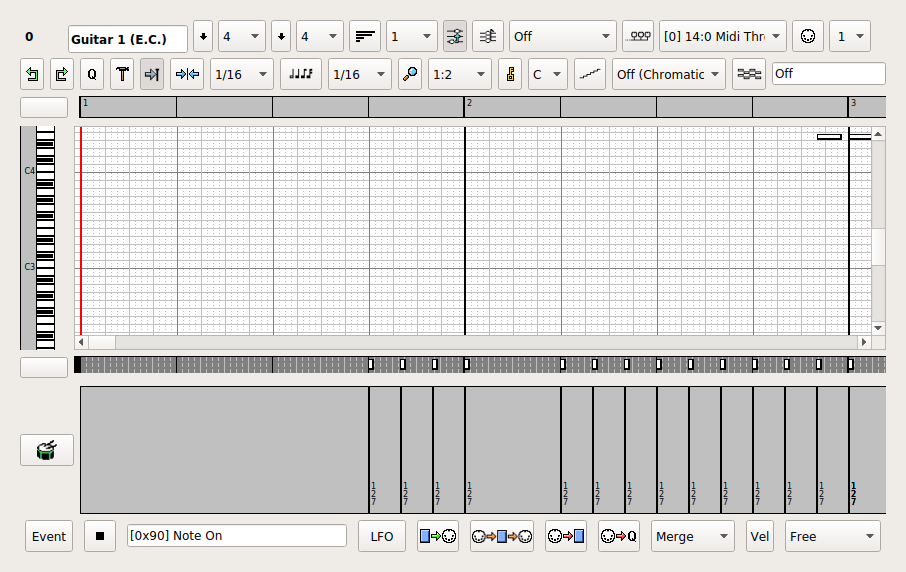
\includegraphics[scale=0.65]{roll.png}
   \caption*{"New Version"}
\end{figure}

\clearpage                             % moves Contents to next page

\tableofcontents
\listoffigures                         % print the list of figures
\listoftables                          % print the list of tables

% Changes the paragraph style to remove indenting and put a line between each
% paragraph.  This could be moved up into the preamble, but then would
% affect the spacing of the TOC and LOF, LOT noted above.

\setlength{\parindent}{2em}
\setlength{\parskip}{1ex plus 0.5ex minus 0.2ex}

\section{Introduction}
\label{sec:introduction}

   This document describes \textsl{Sequencer66}
   \cite{sequencer66}, through version 0.90.0.
   The following project supports \textsl{Sequencer66}:

   \begin{itemize}
      \item \url{https://github.com/ahlstromcj/sequencer66.git}.
      \item \url{https://github.com/ahlstromcj/sequencer64-doc.git}.
   \end{itemize}

   We include the old \textsl{Sequencer64} documentation project because we would
   like a more lean-and-mean manual for \textsl}Sequencer66].

   \textsl{Sequencer66} is \textsl{Sequencer64} refactored for newer versions of
   \textsl{C++} and with a lot of kruft removed.  It drops the Gtkmm
   user-interface in favor of \textsl{Qt 5} and has better handling of sets and
   configuration files.

   We have many contributors to acknowledge.  Please see
   \sectionref{sec:kudos}.

\subsection{Sequencer66: What?}
\label{subsec:what_is_sequencer66}

   \textsl{Sequencer66} is an ongoing reboot of \textsl{Seq24},
   a live-looping sequencer with an interface more like a hardware sequencer
   than track-based MIDI sequencers.
   \textsl{Sequencer66} is not a synthesizer.  It requires a hardware
   synthesizer, or a software synthesizer such as Timidity \cite{timidity},
   FluidSynth \cite{fluidsynth}, etc.

\subsection{Sequencer66: Why?}
\label{subsec:introduction_seq66_vs_others}

   The first reason to refactor \textsl{Sequencer64} is ...

\subsection{Improvements}
\label{subsec:improvements}

   The following improvements are some that have been made in
   \textsl{Sequencer66} versus \textsl{Sequencer64}.

   \begin{itemize}
      \item A mutes editor.
      \item A sets editor.
      \item A better live frame (main window).
      \item More to write!!!
   \end{itemize}

   For developers, \textsl{Sequencer66} is customizable via C macros,
   by enabling/disabling options at build-configuration time, and by many
   command-line arguments.  We cannot show all permutations of settings in this
   document, so don't be surprised if some screenshots don't quite match
   one's setup.  Distro maintainers might pick their favorite build
   configurations.

\subsection{Document Structure}
\label{subsec:introduction_document_structure}

   The structure of this document follows the user-interface of
   \textsl{Sequencer66}.  The sections are provided in the order
   their contents appear in the user-interface of \textsl{Sequencer66}.  To
   help the reader jump around this document, it provides
   multiple links, references, and index entries.

\subsection{Let's Go!}
\label{subsec:introduction_lets_get_started}

   Make sure no other sound application is running, for the first run.
   Start \textsl{Sequencer66} to use JACK for MIDI, or
   on \textsl{Windows}, just run it (\texttt{qpseq66.exe};
   on \textsl{Windows}, PortMidi is used). The port
   settings will be different.  Provide a MIDI file.
   On our system, the synthesizer
   (\textsl{Yoshimi}) comes up on MIDI buss 5; an option remaps
   all events to that buss:

\begin{verbatim}
   $ seq66 --jack-midi --buss 5 contrib/midi/b4uacuse-seq24.midi
   C:\> qpseq66 --buss 1  contrib/midi/b4uacuse-seq24.midi
\end{verbatim}

   If the \texttt{--alsa} option is used instead of
   \texttt{--jack-midi}, then the "JACK" button shows "ALSA" instead
   (Linux only).  The following figure is for the Linux
   version.

\begin{figure}[H]
   \centering 
%  \includegraphics[scale=0.5]{new/seq66-first-screen-0-94.png}
   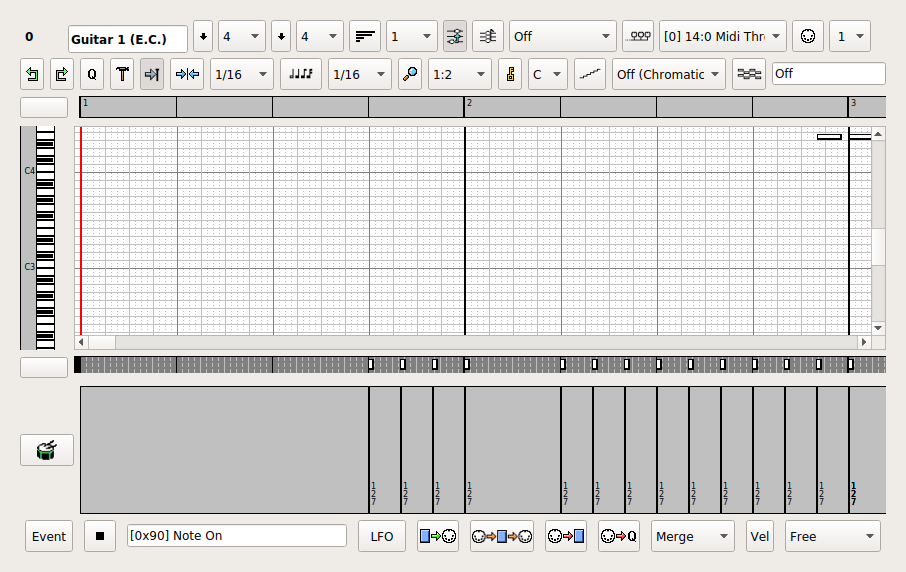
\includegraphics[scale=0.65]{roll.png}
   \caption{Sequencer66 Main Screen, Linux ALSA MIDI}
   \label{fig:seq66_main_screen}
\end{figure}

   The following figure shows the user-interface used for
   \textsl{Windows}.  It uses the Qt 5 framework.

\begin{figure}[H]
   \centering 
%  \includegraphics[scale=0.65]{new/seq66-first-screen-0-96-qt.png}
   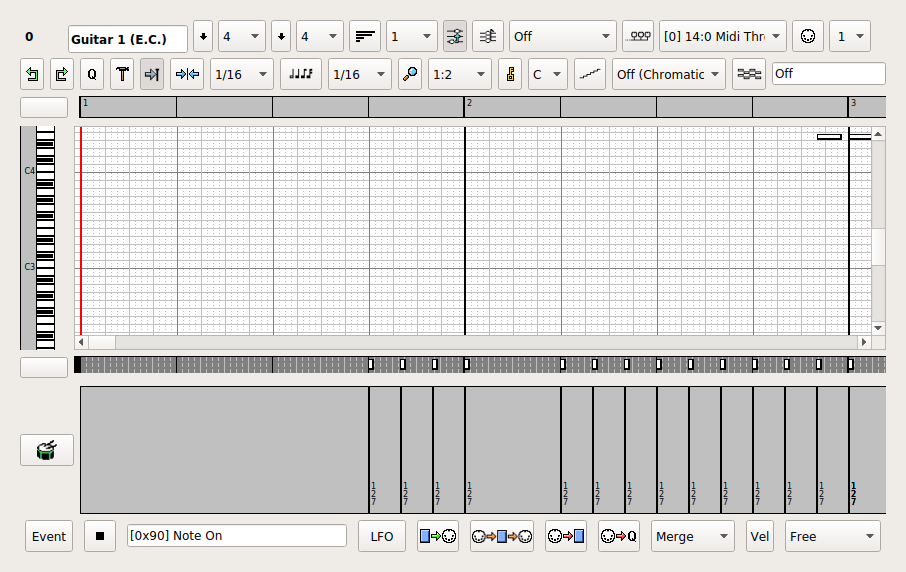
\includegraphics[scale=0.65]{roll.png}
   \caption{Sequencer66 Main Screen, Qt 5 Interface, With Colors}
   \label{fig:seq66_main_screen_qt}
\end{figure}

   The \textsl{Sequencer66} main window appears, as shown above.
%  \figureref{fig:seq66_main_screen}, and
%  \figureref{fig:seq66_main_screen_qt}.
   These figures have some differences from the \textsl{Seq24} main window
   and from each other, but the functionality is about the same.
   Most features, including the "look" of the application,
   can be configured via the "rc" and "user"
   configuration files or command-line options.
   There are many new front-panel items in \textsl{Sequencer66}, but
   the Qt and Gtkmm user-interfaces differ in details.

   \begin{itemize}
      \item Control buttons:
      \begin{itemize}
         \item Start, Stop, and Pause.
         \item Toggle and show the status of "Live" mode versus "Song" mode.
         \item Mute/show the mute status of all tracks.
         \item Enable/disable the menu bar and show its status.
         \item Set JACK Slave/Master transport, and
            ALSA/JACK (native) mode.
         \item Set the kind of time display, between "bars:beat:ticks"
            and "hours:minute:seconds".
         \item Panic button, to stop all tracks and turn off all notes.
         \item Song-recording snap, the \textbf{S} button.
         \item Tap Tempo, the \textbf{0} (zero) button.
         \item Keep-queue toggling and status.
      \end{itemize}
      \item Current time in bars, beats, and ticks.
      \item Song recording records all muting changes to the Song Editor.
      \item Log Tempo, which inserts the current tempo into the tempo track
         as an event.
      \item Tempo recording, which inserts all tempo changes as tempo events.
   \end{itemize}

   Many of these buttons have configurable keystrokes as well.
   See \sectionref{subsec:seq66_patterns_panel_bottom}.
   Some of these items are not present in the Qt interface.

\rhead{\rightmark}         % shows section number and section name

% Menu

%-------------------------------------------------------------------------------
% seq66_menu
%-------------------------------------------------------------------------------
%
% \file        seq66_menu.tex
% \library     Documents
% \author      Chris Ahlstrom
% \date        2015-08-31
% \update      2019-08-20
% \version     $Revision$
% \license     $XPC_GPL_LICENSE$
%
%     Provides the Menu section of sequencer66-user-manual.tex.
%
%-------------------------------------------------------------------------------

\section{Menu}
\label{sec:seq66_menu}

   The \textsl{Sequencer66} menu
   (\figureref{fig:seq66_main_screen}) is simple, but important.

\subsection{Menu / File}
\label{subsec:seq66_menu_file}

   The \textbf{File} menu is used to save and load MIDI files
   (Standard MIDI Format 0 or 1) and \textsl{Sequencer66} MIDI
   files.
   The \textsl{Sequencer66} menu entry contains the sub-items shown below.
%  \figureref{fig:seq66_menu_file_items}.
   The next few sub-sections discuss
   the sub-items in the \textsl{File} sub-menu.

\begin{figure}[H]
   \centering 
   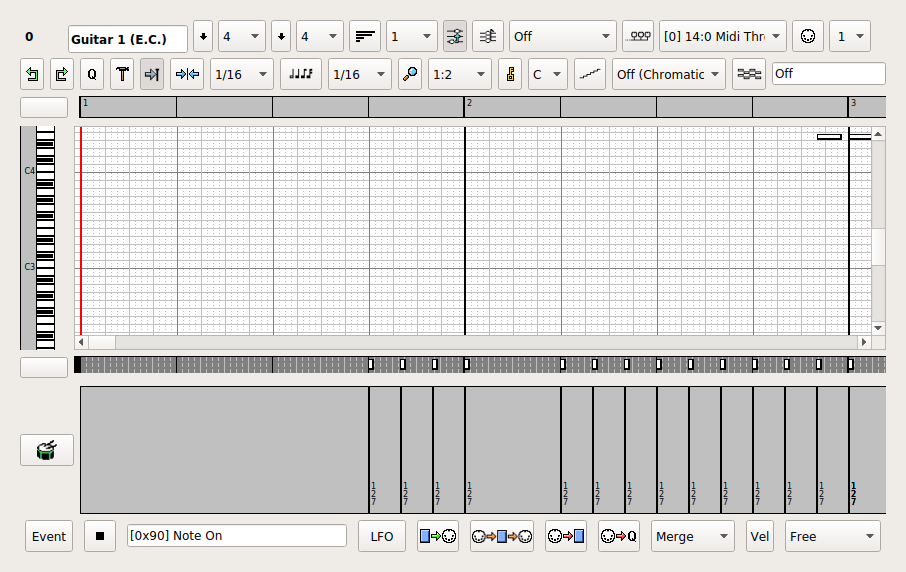
\includegraphics[scale=0.65]{roll.png}
   \caption{Sequencer66 File Menu Items}
   \label{fig:seq66_menu_file_items}
\end{figure}

   \begin{enumber}
      \item \textbf{New}
      \item \textbf{Open}
      \item \textbf{Open Playlist}
      \item \textbf{Recent MIDI files}
      \item \textbf{Save}
      \item \textbf{Save As}
      \item \textbf{Export Song as MIDI}
      \item \textbf{Export MIDI Only}
      \item \textbf{Import MIDI to Current Set}
%     \item \textbf{Options}
      \item \textbf{Exit or Quit}
   \end{enumber}

%  The Qt version of this menu is similar, except that the
%  \textbf{Options...} menu is placed in \textbf{Edit / Preferences}.

\subsection{Menu / File / New}
\label{subsec:menu_file_new}

   The \textbf{New} menu entry clears out the current song or play-list.
   If unsaved changes are pending, the user is prompted to save the changes.
   Prompting for changes is more comprehensive than \textsl{Seq24}.
   However, when in doubt, save!  Keep backups of your tunes!

\subsubsection{Menu / File / Open}
\label{subsubsec:seq66_menu_file_open}

   The \textbf{Open} menu entry opens a song (MIDI file or \textsl{Cakewalk}
   WRK file), replacing the current song.
   It opens up a standard Qt 5 file dialog:

\begin{figure}[H]
   \centering 
%  \includegraphics[scale=0.5]{menu/menu_file_open.png}
   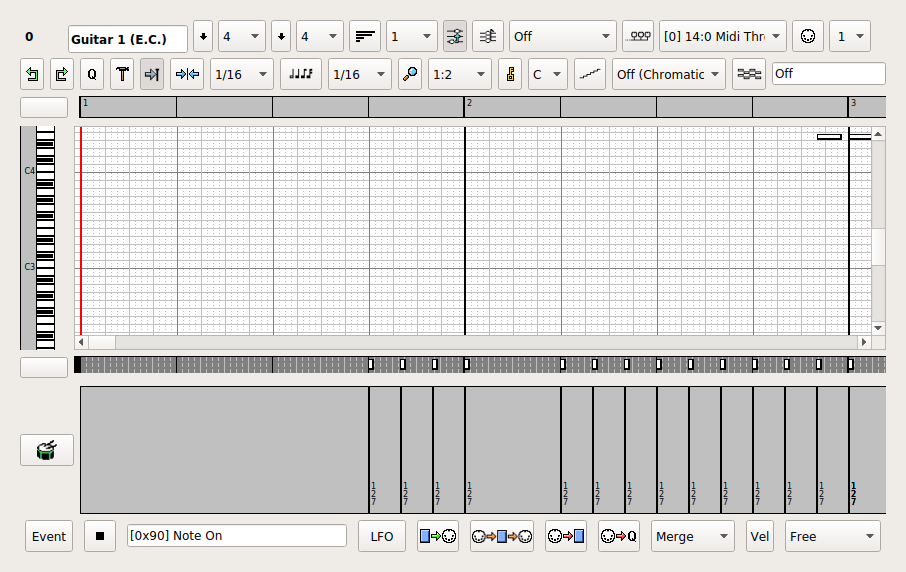
\includegraphics[scale=0.65]{roll.png}
   \caption{File / Open}
   \label{fig:seq66_menu_file_open}
\end{figure}

   This dialog lets one type a file-name, highlighting the first file (if any)
   that matches the characters typed so far.
   \textsl{Sequencer66} can open regular MIDI files and
   Cakewalk WRK files.
   It will read and store some MIDI Meta events 
   (e.g. Tempo and Time Signature).

\subsubsection{Menu / File / Open Playlist}
\label{subsubsec:seq66_menu_file_open}

   The \textbf{Open Playlist...} menu entry opens a \textsl{Sequencer66}
   play-list file.
   This file contains a list of "playlist sections",
   each listing a number of MIDI songs.
   These playlists and songs can be
   selected by the arrow keys or by MIDI control.
   See \sectionref{sec:playlist}.

   Once activated, the current play-list file-name is saved in the
   \texttt{[playlist]} section of the "rc" configuration file when
   \textsl{Sequencer66} exits.
   The file extension is \texttt{.playlist}.
   The Qt user-interface will eventually support editing of the play-list.
   Currently, the user must understand the play-list format, and use a
   text editor to edit the play-list file.

\subsubsection{Menu / File / Recent MIDI files}
\label{subsubsec:seq66_menu_file_recent}

   This menu entry provides a list of the last few MIDI files created or opened;
   play-list selections are \textsl{not} included.
   This list is saved in the \texttt{[recent-files]} section of the
   "rc" configuration file.
   In the menu, only the last part of the file-name is
   shown, but in the "rc" configuration file,
   the full path to the file-name is stored.
   This path is in "UNIX" format, using the forward slash, or solidus,
   as the path separator, even in \textsl{Windows}.
   Only unique entries are included in the recent-files list.
   The limit is 10 recent-file entries.
   This is a feature from \textsl{Kepler34} (\cite{kepler34}).
   Here is an example from an "rc" file:

\begin{verbatim}
   [recent-files]
   # Holds a list of the last few recently-loaded MIDI files.
   3
   /home/chris/git/seq66/data/b4uacuse-gm-patchless.midi
   /home/chris/git/seq66/contrib/midi/colours.midi
   /home/chris/git/seq66/Julian-data/TestBeeps.midi
\end{verbatim}

\subsubsection{Menu / File / Save and Save As}
\label{subsubsec:menu_file_open_save_as}

   The \textbf{Save} menu entry saves the song under its current file-name.
   If there is no current file-name, it opens up a standard file
   dialog to name and save the file.
   The \textbf{Save As} menu entry saves a song under a different name.
   It opens up the following standard file dialog, very similar to the 
   \textbf{File Open} dialog, with an additional \textbf{Name} text-edit field.

\begin{figure}[H]
   \centering 
%  \includegraphics[scale=0.5]{menu/menu_file_save_as.png}
   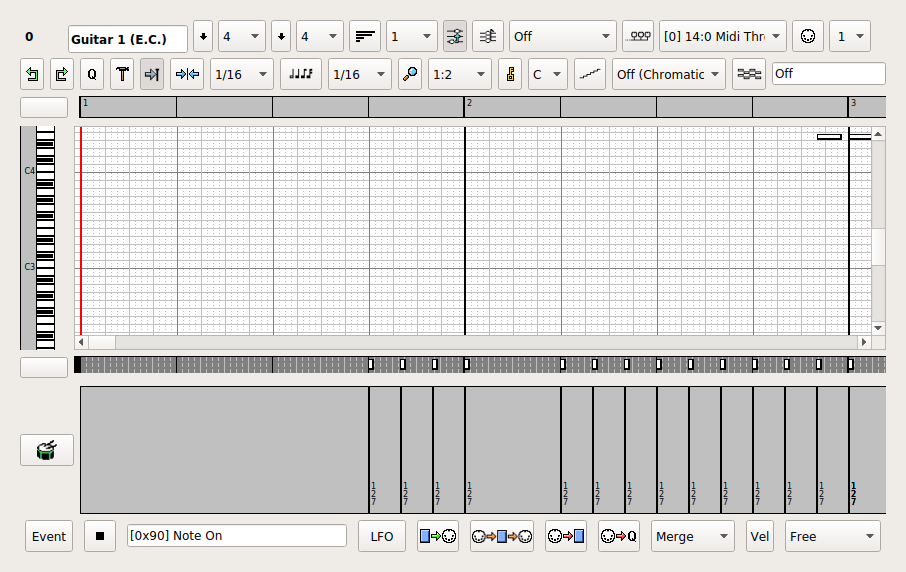
\includegraphics[scale=0.65]{roll.png}
   \caption{File / Save As}
   \label{fig:seq66_menu_file_save_as}
\end{figure}

   To save a new file, or to save the current existing file to a new name,
   enter the name in the name field, without an extension.
   \textsl{Sequencer66} will append a \texttt{.midi} extension to the filename.
   The file will be saved in a format that the Linux \textsl{file} command
   will tag as something like:

   \begin{verbatim}
      myfile.midi: Standard MIDI data (format 1) using 16 tracks at 1/192
   \end{verbatim}

   It looks like a simple MIDI file, and yet, if one re-opens it in
   \textsl{Sequencer66}, one sees that all of the labeling, pattern
   information, and song layout has been preserved in this file.
%  Even the pattern layout (arrangement), as discussed in
%  \sectionref{subsubsec:seq66_song_editor_arrangement_panel_roll},
%  have been saved.
%  (But the L and R marker positions are not saved.)
   This information is saved in a way that MIDI-compliant software
   should be able to use, or ignore without failure.

   The output MIDI file after \textsl{Sequencer66} saves the original MIDI file
   is larger.
   After the last track in the file, a number of
   \index{SeqSpec}
   MIDI-compliant sequencer-specific (SeqSpec) items are saved, to preserve
   the extra information that \textsl{Sequencer66} adds.
   In legacy mode, \textsl{Sequencer66} saves this information
   in the same format as \textsl{Seq24}.
   Otherwise, it saves it in a more MIDI-compatible format.
%  Some of this extra information (mute-groups) will be stripped from the MIDI
%  file.
   Normally, \textsl{Sequencer66} saves this information by marking
   each SeqSpec section as vendor-specific information, and marking this
   section as a regular MIDI track.
   The legacy and new formats of the final "track" are explained in
   \sectionref{subsec:legacy_midi_format}.

   \index{Meta events}
   Meta events are now partially handled by \textsl{Sequencer66}.
   Meta events Set Tempo
%  (\texttt{FF 51 03 tt tt tt}),
   and Time Signature
%  (\texttt{FF 58 04 nn dd cc bb}),
   are now fully supported.
   Other Meta events,
   such as Meta MIDI Channel
%  (\texttt{FF 20 01 cc}),
   and Meta MIDI Port
%  (\texttt{FF 21 01 pp}),
   are now read as events, and are saved back when the file is saved.
   They cannot be edited in \textsl{Sequencer66}, but they are
   not lost.
   Please note that the channel and port meta events are
   considered \textsl{obsolete} in the MIDI standard.

\subsubsection{Menu / File / Import MIDI}
\label{subsubsec:seq66_menu_file_import}

   The \textbf{Import} menu entry imports an SMF 0
   or SMF 1 MIDI file as one or more patterns, one pattern per track,
   into the specified screen-set.
   This functionality is explained in detail in
   \sectionref{subsec:seq66_midi_export_file_import}.

\subsubsection{Menu / File / Export Song as MIDI}
\label{subsubsec:seq66_menu_file_export}

   Thanks to the \textsl{Seq32} project, the ability to export songs to MIDI
   format has been added.  In this export, a complete song performance is
   recoded so that other MIDI sequencers can play the performance properly.
   This functionality is explained in detail in
   \sectionref{subsec:seq66_midi_export_file_export}.

\subsubsection{Menu / File / Export MIDI Only}
\label{subsubsec:seq66_menu_file_export_midi_only}

   Sometimes it might be useful to export only the non-sequencer-specific
   (non-SeqSpec) data from a \textsl{Sequencer66} song, in order to reduce the
   size of the file or to accomodate non-compliant sequencers.
   This functionality is explained in detail in
   \sectionref{subsec:seq66_midi_export_file_export_midi_only}.

\subsubsection{Menu / File / Options}
\label{subsubsec:seq66_menu_file_options}

   In the \textsl{Portmidi / Windows / Qt 5} version of
   \textsl{Sequencer66}, the \textbf{Options} dialog has been moved to 
   \textbf{Edit / Preferences}.
   See \sectionref{subsubsec:qt_portmidi_qt5_edit_prefs}.
   There are still a few configuration items yet to be represented in that
   new user-interface.

   \textbf{Options} provides a number of settings in one
   tabbed dialog, shown in the figures that follow.
   It allows one to set MIDI clocking,
   what incoming MIDI events control the sequencer, what keys are
   mapped to functions, how the mouse works, and some JACK parameters.
   Note that there is a new tab-page for \textbf{Ext Keys}, to support
   more keystroke controls.

\begin{figure}[H]
   \centering 
%  \includegraphics[scale=0.65]{menu/options-tab-0-9-18.png}
   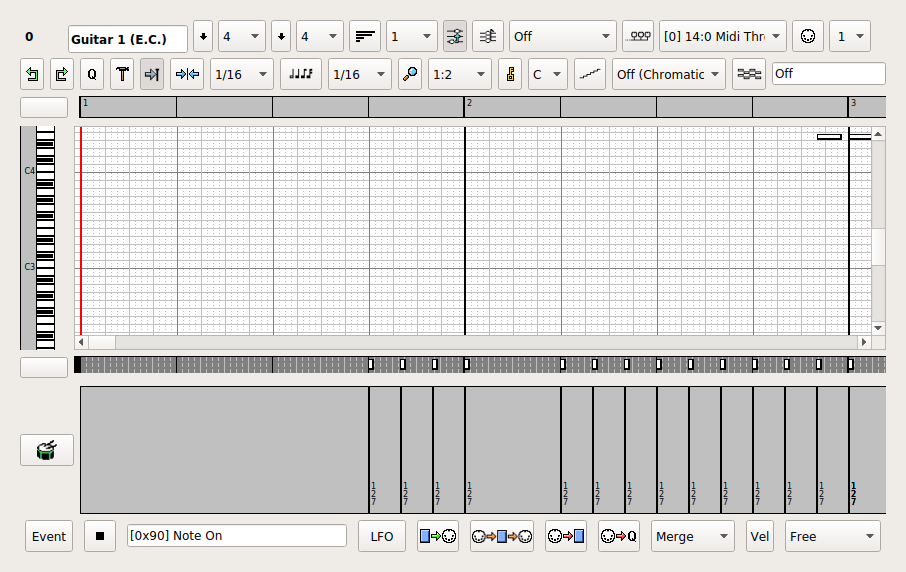
\includegraphics[scale=0.65]{roll.png}
   \caption{Edit / Preference}
   \label{fig:seq66_options_tab_0_9_18}
\end{figure}

\paragraph{Menu / File / Options / MIDI Clock}
\label{paragraph:seq66_menu_file_options_midi_clock}

   The \textbf{MIDI Clock} tab provides a way to set MIDI clock for
   the available MIDI output busses.
   It configures to what busses the MIDI clock and data gets dumped.
   It also shows the devices that can play music.
   The items that appear in this tab depend the setup.

   \begin{itemize}
      \item What MIDI devices are connected to the computer.
         MIDI controllers, USB MIDI cables, applications with virtual
         ports, and other connected devices will add MIDI
         output devices (ports) to the system.
         In \textsl{Windows}, the available devices are shown as well.
%     \item What MIDI software applications are running on the computer.
%        For example, running MIDI software synthesizers such as
%        \textsl{Timidity} and \textsl{Yoshimi} will add extra output devices
%        (playback ports) to a system.
      \item The setting of the "manual ALSA ports" option, which tells
         \textsl{Sequencer66} to set up virtual MIDI ports.
         It is enabled by the
         \texttt{--manual-alsa-ports} command-line option or the
         \texttt{[manual-alsa-ports]} section of the
         \texttt{sequencer66.rc} configuration file, described in
         \sectionref{subsec:seq66_rc_file_manual_ports}.
      \item The setting of the \textsl{Sequencer66}-specific
         "reveal ALSA ports" option,
         \texttt{--reveal-alsa-ports} command-line option or the
         \texttt{[reveal-alsa-ports]} section of the
         \texttt{sequencer66.rc} configuration file, described in
         \sectionref{subsec:seq66_rc_file_reveal_ports}.
   \end{itemize}

   For the current discussion, a USB MIDI cable was plugged into the system,
   and the \textsl{Timidity} and \textsl{Yoshimi} (in ALSA mode) software
   synthesizers were running.  \textsl{Sequencer66} was also running,
   without virtual ports enabled, and \texttt{--alsa} turned on.
%  with the option of "manual ALSA ports" (\texttt{-m} or
%  \texttt{--manual-alsa-ports}) and ALSA (\texttt{-A} or
%  \texttt{--alsa} turned on.
   Here are the devices shown when running \textsl{aplaymidi}
   from the command-line:

   \begin{verbatim}
      $ aplaymidi -l
       Port    Client name                      Port name
       14:0    Midi Through                     Midi Through Port-0
       24:0    E-MU XMidi1X1 Tab                E-MU XMidi1X1 Tab MIDI 1
      128:0    TiMidity                         TiMidity port 0
      128:1    TiMidity                         TiMidity port 1
      128:2    TiMidity                         TiMidity port 2
      128:3    TiMidity                         TiMidity port 3
      129:0    seq66                            seq66 in
   \end{verbatim}

%     129:16   sequencer66                      sequencer66 in

   Note that \textsl{Yoshimi} does not appear.  Perhaps
   \texttt{aplaymidi} does not subscribe properly to all ALSA notifications.
   \textsl{Sequencer66} will detect it.
   One can also run the following command instead:

   \begin{verbatim}
      $ aconnect -io
   \end{verbatim}

   One other note... of late, we're seeing cases where running the
   \textsl{Timidity} daemon hides \textsl{Yoshimi}.  Just be aware.

%  (For some reason, the \textsl{Yoshimi} input port is not showing up
%  in the output of \texttt{aplaymidi}, though, as shown in
%  \figureref{fig:seq66_midi_clock_4_devices_manual_0},
%  \textsl{Sequencer66} sees it on port 7.  Perhaps that application is not
%  providing a good ALSA device name.)
%
%  Also, currently we do NOT see sequencer66/seq66 in the output shown
%  above!  What's up with that!?  Need the -m option!

   Turning to \figureref{fig:seq66_midi_clock_4_devices_manual_1},
   with the option of "manual ALSA ports" (\texttt{-m} or
   \texttt{--manual-alsa-ports}) and ALSA in force,
   note the 16 devices provided by \textsl{Sequencer66}.
%  Also note that its first value is 1, not 0, due to
%  the MIDI Thru port occupying slot 0.
   This figure shows the result with the "manual ALSA option" turned on.
   Remember that this option also applies to the native JACK MIDI
   mode of \textsl{Sequencer66}.

%  Also note that the new \textbf{Port Disabled} radio button is not shown in
%  here.
%  See \sectionref{fig:qt5_prefs_clock_windows}, it shows this button.
%  It was added because Windows can have issues with its built-in MIDI mapper,
%  causing some ports to be uninitialized, and hence not available.
%  We need to ignore those ports.

\begin{figure}[H]
   \centering 
%  \includegraphics[scale=0.75]{menu/midi-clock-4-devices-manual-1.png}
%  \includegraphics[scale=0.75]{new/midi-clock-4-devices-manual-1.png}
%  \includegraphics[scale=0.65]{jack/jack-nano-yosh-manual-clock-seq66.png}
   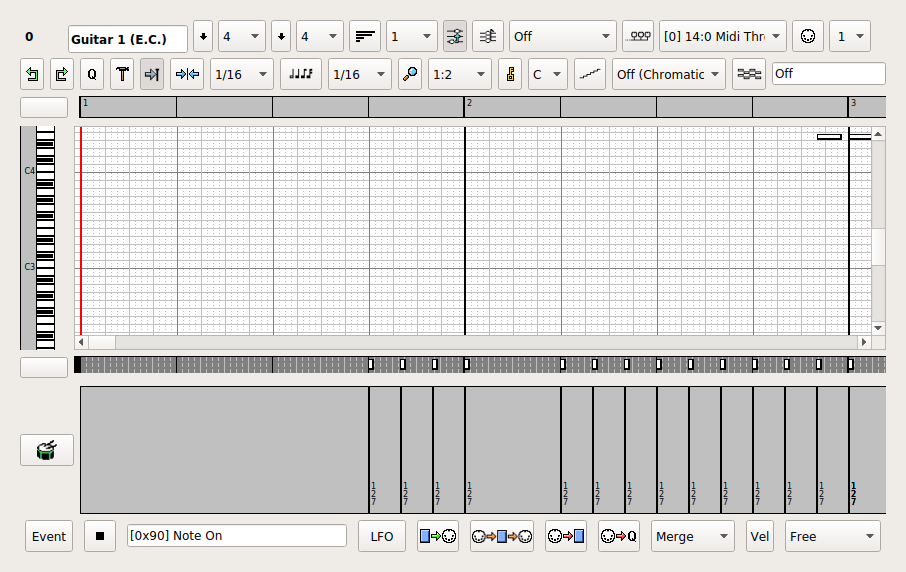
\includegraphics[scale=0.65]{roll.png}
   \caption{MIDI Clock, Manual Option On}
   \label{fig:seq66_midi_clock_4_devices_manual_1}
\end{figure}

   It shows the 16 virtual MIDI output busses that \textsl{Sequencer66} can
   drive.  One needs to use a JACK or ALSA MIDI
   connection application to connect a device on each of those outputs.  The
   fact that the the buss names can
   start with different numbers, depending on the system setup, can complicate
   the playing of MIDI in this manner.  Also, the "user" configuration file can
   change the visible names of the ports, causing further confusion.
   The following elements are present in this dialog:

   \begin{enumber}
      \item \textbf{Index Number}
      \item \textbf{Client Number}
      \item \textbf{Port Number}
      \item \textbf{Buss Name}
      \item \textbf{Port Disabled}
      \item \textbf{Off}
      \item \textbf{On (Pos)}
      \item \textbf{On (Mod)}
      \item \textbf{Clock Start Modulo}
   \end{enumber}

   The format of the left side of the entry listing is like the following:

   \begin{verbatim}
      [4] 4:4 seq66 midi out 4:5
       ^  ^ ^ ^
       |  | | |
       |  | |  -------- Buss name
       |  |  ---------- Port number
       |   ------------ Client number
        --------------- Index number
   \end{verbatim}

   \setcounter{ItemCounter}{0}      % Reset the ItemCounter for this list.

   \itempar{Index Number}{midi clock!index number}
   \index{index number}
   The number in square brackets is an ordinal indicating the position
   of the output buss in the list.
   \index{buss override}
   It can be used with the \texttt{-b --buss --bus} option to redirect all
   output to that one buss, which is useful if only one buss is active, and the
   \textsl{Sequencer66} MIDI song patterns route to non-existent busses.

   \itempar{Client Number}{midi clock!client number}
   \index{client number}
   The number that precedes the colon is the "client number".
   It is useful mainly in ALSA, where clients can have numbers like "14",
   "128", "129", etc.  For native JACK mode, it matches the index number.

   \itempar{Port Number}{midi clock!port number}
   \index{port number}
   The number that follows the colon is the "port number".
   It is useful mainly in ALSA.
   For native JACK mode, it matches the index number.

   \itempar{Buss Name}{midi clock!buss name}
   \index{port name}
   \index{midi clock!port name}
   These labels indicate the output busses (ports) of \textsl{Sequencer66}.
%  They range from \textbf{[1] sequencer66 1} to \textbf{[16] sequencer66 16}
%  in the legacy application, \texttt{sequencer66}.
   They range from \textbf{[1] seq66 1} to \textbf{[16] seq66 16}.
   in native JACK, when manual/virtual ports are active.

   \itempar{Port Disabled}{midi clock!port disabled}
   The \textbf{Port Disabled} clock choice marks a port
   that one does not want to use or that the operating system
   (\textsl{Windows}, I'm looking at \textsl{you}!)
   is locking or disabling that output port.
   Normally, this inaccessible port would cause \textsl{Sequencer66} to exit.
   With the port disabled, the inaccessible port is ignored.

   When the \textsl{Windows} version of \textsl{Sequencer66}
   (\texttt{qpseq66} is first started, it may error out.
   It will then write "erroneous.rc" and "erroneous.usr" configuration
   files, which can be examined to find the offending buss.
%  See \sectionref{fig:qt5_prefs_clock_windows}, it shows this
%  new feature.

   \itempar{Off}{midi clock!off}
   Disables the MIDI \textsl{clock} for the given output buss.
   MIDI output is still sent to those ports, and
   each port that has a device connected to it will play music.
   Some synthesizers may require this setting.
%  For feeding \textsl{Yoshimi} (running in ALSA mode)
%  with MIDI data, we found that this
%  setting is the one that must be made in order for \textsl{Yoshimi} to
%  produce a sound.

   \itempar{On (Pos)}{midi clock!on (pos)}
   MIDI clock will be sent to this buss.
   MIDI Song Position and MIDI Continue will be sent if playback starts
   at greater than tick 0 in Song mode.  Otherwise, MIDI Start will be sent.

   \itempar{On (Mod)}{midi clock!on (mod)}
   MIDI clock will be sent to this buss.
   MIDI Start will be sent, and clocking will begin
   once the Song Position has reached the start modulo of the specified size
   (see the next item's description).
   This setting is used for gear that does not respond to Song Position.

   \itempar{Clock Start Modulo}{midi clock!clock start modulo}
   Clock Start Modulo (1/16 Notes).
   This value starts at 1 and ranges up to 16384, and defaults to 64.
   It is used by the \textbf{On (Mod)} setting discussed above.
   It is the \texttt{[midi-clock-mod-ticks]} option in the \textsl{Sequencer66}
   "rc" file as described in
   \sectionref{subsec:seq66_rc_file_midi_cmt}.

   \itempar{Meta Events}{midi clock!meta events}
   \index{tempo-track-number}
   This section consists of one item, the Tempo Track number.
   It allows the user to move the tempo track from pattern 0 to
   another pattern.  Changing this option is not recommended, since track 1 (0)
   is the official track for tempo events, but \textsl{Sequencer66} allows the
   user to record tempo events to another track.  \textsl{Sequencer66} will
   process tempo events in any pattern.
   \textsl{Not supported yet in the Qt user-interface, but
   it can be set manually in the "rc" configuration file.}

   In addition, the \textbf{Set as Song Tempo Track} button sets this
   track as part of the currently-load MIDI song file, and will be saved when
   exited.  This value will override the global tempo-track value, which is
   stored in the 'rc' configuration file.  However, if 0, it will be ignored,
   so that the global value will take hold.
   See \sectionref{subsec:seq66_rc_file_midi_meta_events}, which discusses this
   setting in the "rc" configuration file.

   One thing to remember about tempo...
   there is a "global" tempo which is saved as part of the song in a SeqSpec
   section.  However, that tempo is not saved in the tempo track.
   In order to do so, one can click the \textbf{Log Tempo} button to write it
   to the tempo track as a tempo event.

\begin{figure}[H]
   \centering 
%  \includegraphics[scale=0.75]{menu/midi-clock-4-devices-manual-0.png}
%  Updated for version 0.93.1:
%  \includegraphics[scale=0.65]{new/midi-clock-4-devices-manual-0.png}
   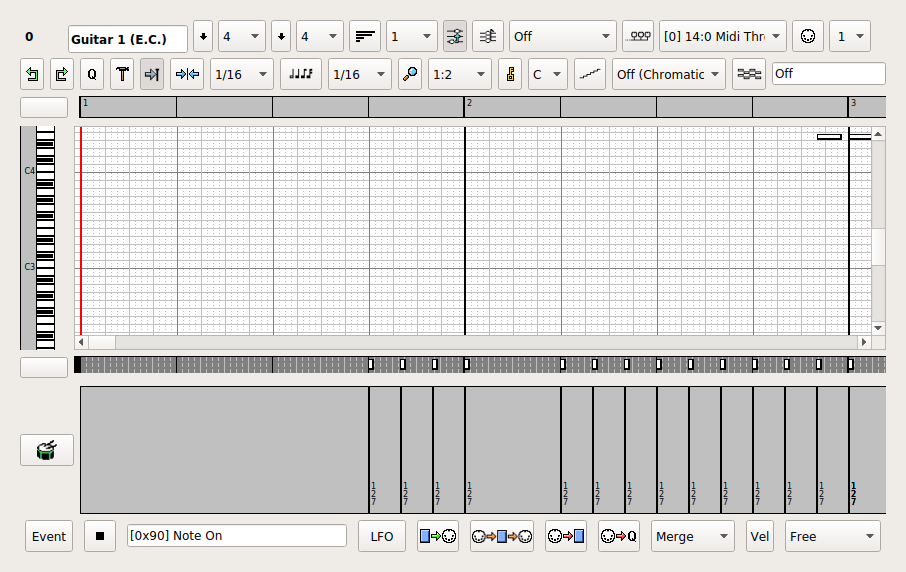
\includegraphics[scale=0.65]{roll.png}
   \caption{MIDI Clock, Manual Option Off (ALSA View, Old Screenshot)}
   \label{fig:seq66_midi_clock_4_devices_manual_0}
\end{figure}

   In the figure above, with the "manual ALSA option" is turned off, and
   all of the real (non-virtual) devices that can be driven by MIDI output are
   shown, including the MIDI Thru port, and
%  the MIDI port on the \textsl{E-MU XMidi1x1} USB cable,
   the four ports provided by \textsl{Timidity} on our setup.
%  , and the unlabelled
%  port provided by the \textsl{Yoshimi} synthesizer running in ALSA mode.
%  (However, \texttt{seq66} does show the name "yoshimi" as the client name.)
%  One could theoretically play music through 6 or 7 devices using
%  \textsl{Sequencer66} with this setup.
   (The \textbf{Port Disabled} column is missing from this old screenshot.  We
   need to fix that someday.)

   See \sectionref{subsec:seq66_jack_native_midi},
   for a lot more information about native JACK support, and examples of JACK
   MIDI ports and connections.

   \index{todo!manual alsa gui option}
   There is currently no user-interface item corresponding to the "manual ALSA"
   command-line and "rc" configuration file option.
   We should rename this option to "virtual"
   eventually, since it can also apply to JACK MIDI.

\paragraph{Menu / File / Options / MIDI Input}
\label{paragraph:seq66_menu_file_options_midi_input}

   To allow \textsl{Sequencer66} to record MIDI from MIDI devices such as
   controllers and keyboards, the output of the ALSA MIDI recording
   command-line application is relevant:

   \begin{verbatim}
      $ arecordmidi -l
       Port    Client name                      Port name
       14:0    Midi Through                     Midi Through Port-0
       24:0    USB2.0-MIDI                      USB2.0-MIDI MIDI 1
      129:1    seq66                            seq66 midi out 0
      129:2    seq66                            seq66 midi out 1
       . . .   . . .                               . . .
      129:16   seq66                            seq66 midi out 15
   \end{verbatim}

% Should the above be offset re 0, not 1?  Check it out!!!

   We see that we can record MIDI from the MIDI Thru port, from the USB MIDI
   cable, and MIDI from any of the 16 output ports provided by the manual ALSA
   port mode of \textsl{Sequencer66}.

   If the "manual ALSA ports" option is turned \textsl{off} (e.g. by using the
   \texttt{-a} option),
   then the only item in the \textbf{MIDI Input} tab is the single MIDI input
   buss provided by \textsl{Sequencer66}:  \textbf{[0] seq66 0}.
   (The figure shown is currently out-of-date.)

% Should the above be offset re 0, not 1?  Check it out!!!

\begin{figure}[H]
   \centering 
%  \includegraphics[scale=0.75]{menu/midi-input-4-devices-manual-1.png}
%  \includegraphics[scale=0.65]{new/midi-input-4-devices-manual-1.png}
   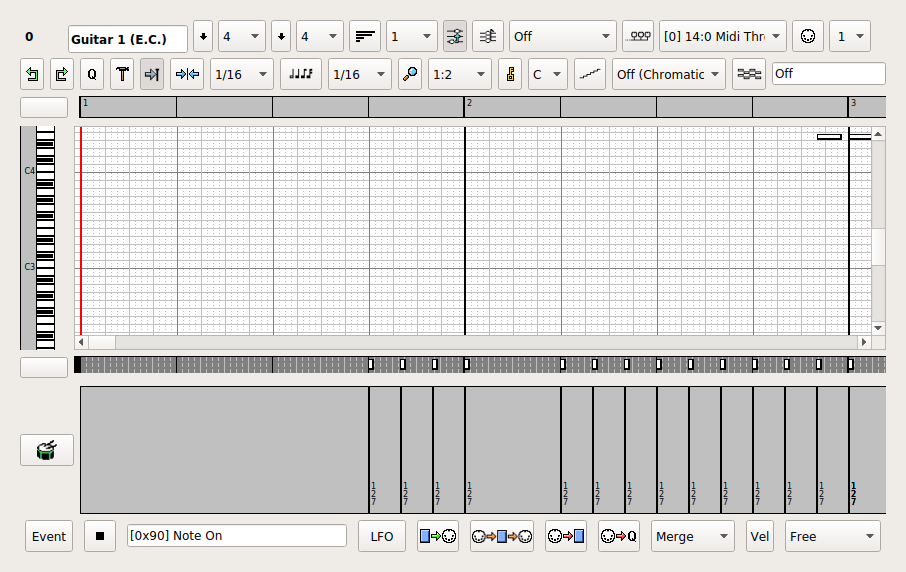
\includegraphics[scale=0.65]{roll.png}
   \caption{MIDI Input, Manual Ports Off (Condensed View)}
   \label{fig:seq66_midi_input_4_devices_manual_1}
\end{figure}

% WE NEED a composite view of the -m, -A, and -a options for ALSA for
% both the Clock and the Input tabs!!!!!

% Check the following out!  I am not 100% certain it is correct!!!
% The above is shown with the -A option.

   Any item checked allows \textsl{Sequencer66} to record MIDI
   from another source,
   which must be connected to this port via
   another application).
%  , or pass it through to the output busses
%  that are configured to allow pass-through
%  (in the Pattern Editor, as discussed in 
%  \sectionref{subsec:seq66_pattern_editor_bottom}.)

   \textbf{Warning:}
   \index{warnings!usr config}
   \index{usr config}
   If the 
   \texttt{[user-midi-bus-definitions]} value in the "user" configuration file
   is non-zero, and the
   corresponding number of
   \texttt{[user-midi-bus-N]} settings are provided, then
   the list of existing hardware will be ignored, and those values will be
   shown instead.
   (This feature can be overridden with the
   \texttt{--reveal-alsa-ports} (\texttt{-r}) option.)

%  New in \textsl{Sequencer66} is the option to record MIDI input into
%  more than one pattern based on the MIDI channel, as discussed below.

   If the "auto ALSA ports" option is turned on, via the \texttt{-a} or
   \texttt{--auto-alsa-ports} option, then
   the input ports from the system are shown:

\begin{figure}[H]
   \centering 
%  \includegraphics[scale=0.75]{menu/midi-input-4-devices-manual-0.png}
%  \includegraphics[scale=0.65]{new/midi-input-4-devices-manual-0.png}
   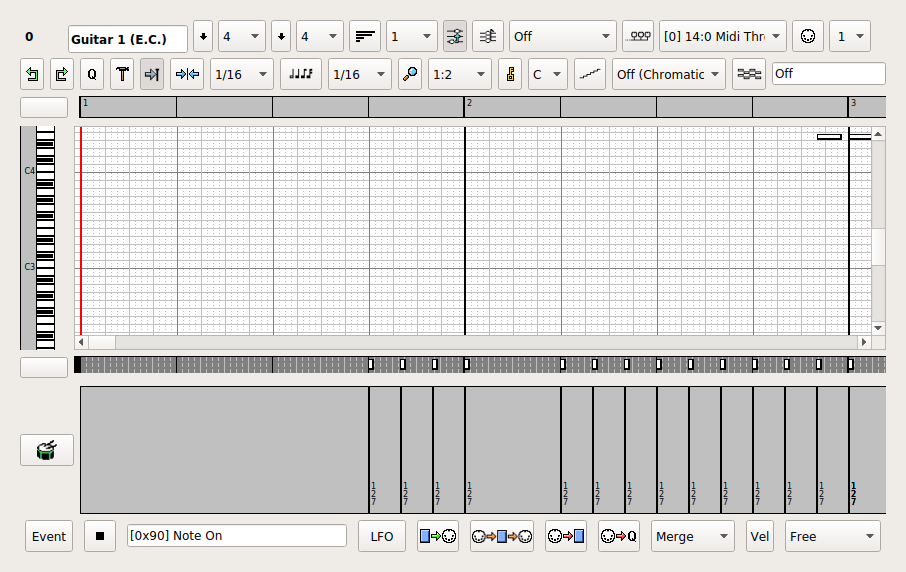
\includegraphics[scale=0.65]{roll.png}
   \caption{MIDI Input, \texttt{-a} Option (Condensed View)}
   \label{fig:seq66_midi_input_4_devices_manual_0}
\end{figure}

   For example, one could check input \#1 to have \textsl{Sequencer66} record
   MIDI from an old-fashioned MIDI keyboard that is connected to another
   USB MIDI cable (the \textsl{E-MU Xmidi}).  If the keyboard didn't have a
   sound generator, one would also want \textsl{Sequencer66} to pass this MIDI
   on to a sound generator, such as a software or hardware synthesizer attached
   to one of the ports shown in
   \figureref{fig:seq66_midi_clock_4_devices_manual_0}.

   \textbf{Warning:}
   \index{warnings!usr config}
   \index{usr config}
   The "user" configuration file can override what is actually
   displayed as hardware.  If you define these sections, they should match your
   hardware exactly, and your hardware should not change from session to
   session.

   Note the two sections of this configuration page:

   \index{input buses}
   \textbf{Input Buses} delineates the MIDI input devices as noted above.
   \index{input options}
   \textbf{Input Options} adds further refinements to MIDI input.

   \index{input by channel}
   \textbf{Record input into sequence according to channel}
   causes MIDI input with multiple channels to be distributed to
   each sequence according to MIDI channel number.
   When disabled, the legacy recording behavior dumps all data into the current
   sequence, regardless of channel.

%  Needs to be clarified!!!

\paragraph{Menu / File / Options / Keyboard }
\label{paragraph:seq66_menu_file_options_keyboard}

   \textsl{Seq24} allows extensive use of
   keyboard shortcuts to make operations go faster than with a mouse,
   and \textsl{Sequencer66} extends that tradition.
   The \textbf{Keyboard} tab (currently in Gtkmm only)
   allows for the configuration of these keyboard shortcuts.

   These settings can also be modified by editing the appropriate "rc"
   configuration file, stored in one of the following directories, depending on
   the operating system:
   
   \begin{verbatim}
         /home/username/.config/sequencer66
         C:/Users/username/AppData/Local/sequencer66
   \end{verbatim}

   \textbf{Warning:}
   \index{keys!gotchas}
   There are a number of "gotchas" to be aware of when assigning keys to the
   fields in the \textbf{Keyboard} tab:

   \begin{itemize}
      \item This configuration dialog is not yet present in the
         \textbf{Qt 5} version of \textsl{Sequencer66}.  For now,
         one has to edit the "rc" file to configure the keystrokes.
         It is easiest to just use the sample \texttt{qpseq66.rc}
         or \texttt{qseq66.rc} from the
         \texttt{data} directory in the source-code package.
         Another option is to just run \textsl{Sequencer66} the first time and
         tweak the "rc" and "usr" files that are created in the directories
         noted above.
         Internally, the Qt key-codes are remapped to Gtk key-codes.
      \item Whenever one of the text fields in this dialog has the focus (and
         that is usually the case), then
         \textsl{any} keystroke, including keys like
         \texttt{Ctrl},
         \texttt{Alt}, and
         \texttt{Super} (also known as Mod4 or the Windows key),
         can alter the value of a
         field to that of the keystroke.  This change is very easy to do
         accidentally!  \textsf{Use the mouse} to move this window and to click
         its \textbf{OK} button!
      \item Some of the keys traditionally used (or used by default) for
         control have been adapted for other uses, and are not configurable.
         One example is \texttt{Ctrl-L}, which brings up the learn mode
         that can be started using the "L" button or the "glearn"
         (group-learn) MIDI control.
         Some other hard-wired keystrokes are the "arrow" keys or "page
         up/down" keys.
      \item \textsl{Sequencer66} has appropriated the
         \index{keys!shift} Shift key so that it
         modifies a click on a pattern so that all of the other patterns are
         \textsl{toggled}.  Therefore, using characters that require the Shift
         key while clicking, such as \texttt{\{} and \texttt{\}}, when used
         to set the \textbf{Replace} function, becomes surprising.
         Instead, look to the remaining keys: \texttt{F11}, \texttt{F12},
         and the "keypad" keys if more options are wanted.  Be sure to
         look at the \textbf{Ext Keys} tab to see what other keys are in use.
         \index{auto-shift}
         Also, for the group-learn feature, the \texttt{Shift} key is 
         automatically enabled, using an "auto-shift" feature.
   \end{itemize}

\begin{figure}[H]
   \centering 
%  \includegraphics[scale=0.65]{new/menu_file_options_keyboard.png}
   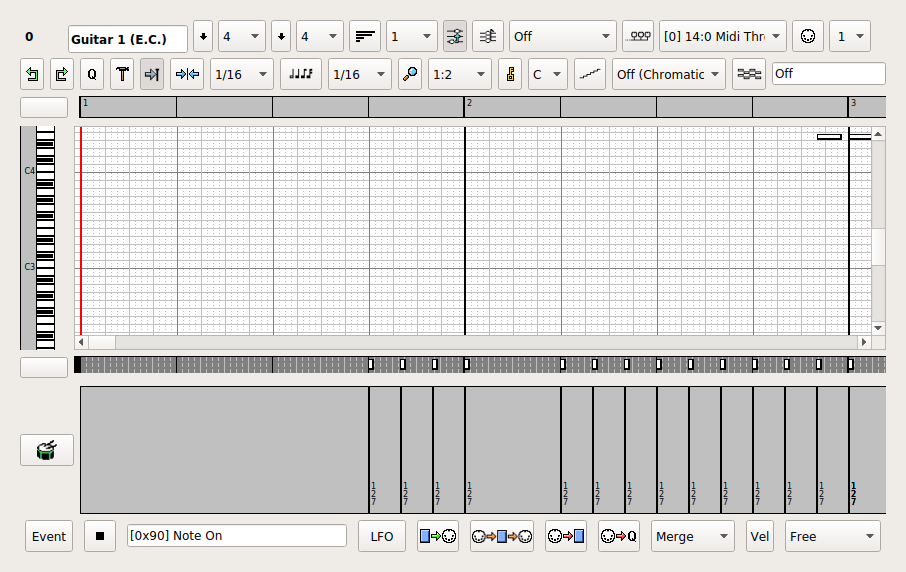
\includegraphics[scale=0.65]{roll.png}
   \caption{File / Options / Keyboard}
   \label{fig:seq66_menu_file_options_keyboard}
\end{figure}

   \texttt{[keyboard-control]}.
   We won't attempt to cover every user-interface item in this busy
   dialog, just the categories.  Some items might be discussed in other parts
   of this manual.

   There are some things to note in the \texttt{[keyboard-control]} section.
   First, it is laid out like the main patterns panel, in an 8 x 4 grid.
   The keys in there correspond directly to the patterns panel slot, and the
   conventional keyboard layout is shown.
   Second, if one is looking for more keys to map to other functions, the
   default layout keeps open the following keys:
   \texttt{9 o l 0 p}.
%  Third, these key-mappings are stored in the
%  \texttt{[keyboard-control]} section of the "rc" configuration file.

   The \texttt{[mute-group]} section is laid out in a similar manner, except
   that the \textbf{upper-case} versions of the keys are used.  Additional keys
   are available for other functions:
   \texttt{( O L ) P}.
   Currently, one must be very carefully about assigning the same key to
   different functions.  Confusion will ensue!  We've done it!
%  Note that these key-mappings are stored in the
%  \texttt{[mute-group]} section of the "rc" configuration file.

%  \index{new!pause}
   \index{pause}
%  If the application has been built with the "pause" option, an
   An additional key definition is shown for the Pause key.
   By default, the Pause key is the period (".").  An old version of
   the "rc" file is automatically fixed to include this new option.
%  (The pause feature can be removed by rebuilding the application
%  after configuring with the \texttt{--disable-pause} option, but
%  why would you want to do that?)

% \begin{figure}[H]
%    \centering 
%    \includegraphics[scale=0.75]{new/keyboard-options-0_9_10_1.png}
%    \caption{File / Options / Keyboard, with Pause}
%    \label{fig:seq66_menu_file_options_keyboard_pause}
% \end{figure}

   \index{pattern edit}
   New features try to achieve being able to edit a pattern using only the
   keyboard.  \textsl{Sequencer66} now supports two modifier keys.
   The first modifier key causes the usual pattern-toggle key (hot-key) for a
   given slot to instead bring up the pattern editor.  By default, this key is
   the equals ("=") key.
   \index{event edit}
   The second modifier key causes the usual
   pattern-toggle key (hot-key) for a given slot to instead bring up the event
   editor.  By default, this key is the minus ("-") key.
   These keys are configurable in the
   \textbf{File / Options / Ext Keys} page.
%  As with the other
%  keys, these keys can be reconfigured to a different set of keys in the
%  \textbf{File / Options / Keyboard} page.

   To continue with a listing of the keyboard options:

   \begin{enumber}
      \item \textbf{Show sequence hot-key labels on sequences}
      \item \textbf{Show sequence numbers on sequences}
      \item \textbf{Control keys [keyboard-group]}
      \item \textbf{Sequence toggle keys [keyboard-control]}
      \item \textbf{Mute-group slots [mute-group]}
      \item \textbf{Learn}
      \item \textbf{Disable}
      \item \textbf{Enable}
   \end{enumber}

   These categories are described below.

   \setcounter{ItemCounter}{0}      % Reset the ItemCounter for this list.

   \itempar{Show key labels on sequence}{keyboard!show labels}
   This option shows the key labels in the lower-right corner of
   each loop/pattern slot in the Patterns window (the main window).
   It is useful for live playback and control of a song.
   It is configurable in the "rc" configuration file.
   It also enables the display of the pattern length, in
   measures, at the top right of the pattern slot.

   \itempar{Show sequence numbers on sequence}{keyboard!sequence numbers}
   \index{new!sequence numbers}
   If this option is on, the
   empty slots in the pattern window show the prospective sequence number.
   See the following figure for one look of this feature.

\begin{figure}[H]
   \centering 
%  \includegraphics[scale=0.75]{pattern-window-with-numbering.png}
%  \includegraphics[scale=0.65]{new/pattern-window-with-numbering.png}
   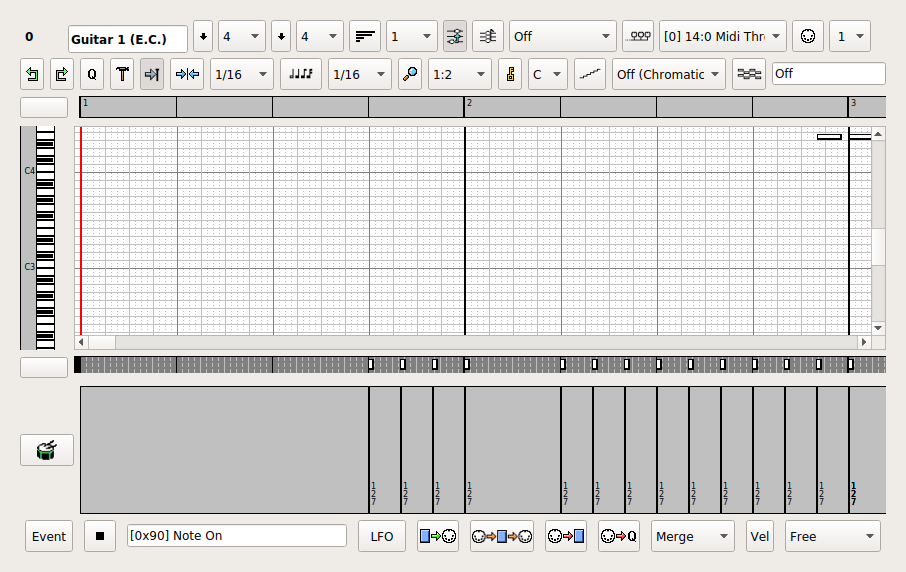
\includegraphics[scale=0.65]{roll.png}
   \caption{Pattern Window with One Kind of Numbering}
   \label{fig:seq66_build_with_numbering}
\end{figure}

   The option also changes the visibility of sequence numbers
   in active sequences and in the Song Editor's names column.
   If one doesn't like it, turn off the option in the "rc" configuration file,
   or try other grid options in the "user" configuration file.

   \itempar{Control keys}{keyboard!control keys}
   \texttt{[keyboard-group]}.
   This block of fields in the \textbf{Options / Keyboard} tab
   provides shortcut keys for many operations of
   \textsl{Sequencer66}.  There is a default mapping built into
   \textsl{Sequencer66}, but open the keyboard options tab to see
   the actual values.
   
%  Some of the old \textsl{Seq24} defaults were ill-advised.

   \begin{enumber}
      \item \textbf{Start}.
      \item \textbf{Stop}.
      \item \textbf{Pause}.
      \item \textbf{Slot Shift}.
      \item \textbf{Snapshot 1}.
      \item \textbf{Snapshot 2}.
      \item \textbf{bpm up}.
      \item \textbf{bpm down}.
      \item \textbf{Replace}.
      \item \textbf{Queue}.
      \item \textbf{Keep queue}.
      \item \textbf{Screenset down}.
      \item \textbf{Screenset up}.
      \item \textbf{Set playing screenset}.
   \end{enumber}

   Some of the keys have positional mnemonic value.  For example,
   for BPM control, the semicolon is at the left (down), and the apostrophe
   is at the right (up).
   Note that the keys definable in this tab are only a subset of the
   various keys that can be used, especially keys used with the
   \texttt{Ctrl} key or other modifier keys.

   \index{slot-shift}
   \index{keys!slot-shift}
   The \textbf{slot shift} key is useful when using pattern grids larger
   than 8 x 4 patterns.  Pressing the slot-shift key basically adds 32 to the
   pattern number of the slot-key that is pressed.
   Not all builds of \textsl{Sequencer66} support this option.

   \index{snapshot}
   \index{keys!snapshot}
   A \textbf{snapshot} is a briefly-preserved state of the patterns.
   One can press a snapshot key, change the state of the patterns for live
   playback, and then release the snapshot key to revert to the state when
   the snapshot key was first pressed.

%  TODO:  Investigate this note from SEQ24:
%
%   Holding 'Alt' will save the state of playing sequences
%   and restore them when 'Alt' is lifted.
%
%   Holding 'Left Ctrl' and 'Alt' at the same time will enable
%   you to flip over to new sequences briefly and then
%   flip right back upon lifting 'Alt'.
%
%	Is this Snapshot 1 versus Snapshot 2?  In Seq24's code, either key
%  does exactly the same thing!


   \index{queue}
   \index{keys!queue}
   To \textbf{queue}
   a pattern means to ready it for playback upon the next repeat
   of a pattern.  A pattern can be armed immediately with a hot-key,
   or it can be queued to play back the next time the pattern repeats.
   A pattern can be queued by holding the queue key (defined in
   \textbf{File / Options / Keyboard / queue}) and pressing a pattern-slot
   hot-key.  Instead of the pattern turning on
   immediately, it turns on at the next repeat of the pattern.

   \index{keep queue}
   \index{keys!keep queue}
   \index{queue!keep}
   \textbf{Keep queue}
   allows the queue to be held without holding
   down the queue button the whole time.  First, press the keep-queue key
   (defined in \textbf{File / Options / Keyboard / Keep queue}).  Now, hitting
   any of the slot hot-keys, no matter how many, sets up the corresponding
   pattern slot to be queued.  Also, in keep-queue mode, clicking on the
   pattern slot will queue the pattern.  The keep-queue mode is disabled by
   hitting the "queue" key again (any currently active queues remain active
   until finished).  There is also a "Q" button to toggle the keep-queue
   status.

   Be sure to note the new option, \textbf{one-shot queue}, in the
   extended-keys section (\sectionref{subsubsec:seq66_patterns_pattern_slot}).

   \itempar{Sequence toggle keys}{keyboard!sequence toggle keys}
   Each of these keys toggles the playing/muting of one of the 32
   loop/pattern boxes.  These keys are layed out logically on the keyboard,
   and can also be shown in each loop/pattern box.  No need to list them all
   here!  Please note that we often call them "shortcut keys" or
   "hot-keys" where the context
   makes it clear that they apply to the armed/unarmed state of a pattern.

   \itempar{Mute-group slots}{keyboard!mute-group slots}
   There can be up to 32 mute-groups.
   \index{playing set}
   When activated, a mute-group
   sets the muted/unmuted status of the current "playing set"
   to the pattern-muting statuses of the selected mute-group.
   Each of these keys operates on the mute-grouping of one of the 32
   stored mute groups.
   These keys are layed out logically on the keyboard.
   No need to list them all here!
   Generally, they are the shifted versions of the
   keyboard keys used as hot-keys for the patterns.
   Note that a mute-group key will be memorized only when
   \textsl{Sequencer66} is in
   \index{group-learn} \textsl{group-learn} mode.

%  \index{mute-group}
%  One thing to explain is just what mute-grouping means.
%  \textsl{Mute groups} are shortcuts to play a defined group of patterns
%  on the current set, while stopping other patterns from the current set, and
%  all patterns from other sets.

   \itempar{Learn}{keyboard!learn}
   \index{group!learn}

   To define the group of patterns for one mute group, press and hold the
   configured Learn key (the \texttt{Insert} key by default,
   the \texttt{Ctrl-L} key, or the "L" button in the user-interface.
   Simultaneously (not needed with the "L" button),
   press one of the mute group keys: \textsl{Sequencer66}
   will save the currently-playing pattern slots into the corresponding mute
   group.
   \index{auto-shift}
   The default mute group keys must be the shifted version of the key,
   but one does not need the \texttt{Shift} key while pressing
   \texttt{Insert} to learn the group, only to trigger it.
   \textsl{Sequencer66} will automatically assign the corresponding key with
   \texttt{Shift} activated.  Try pressing the \texttt{Shift} key in Learn mode
   and see what happens!

%  Now, on some keyboards (like the author's), 
%  the \texttt{Insert} key is a clumsy two-key button.  So, an alternative
%  is to click the \index{L button} \textbf{L button} and release it,
%  then hit the desired mute-group (no need for the \texttt{Shift} key).
%  One can also press \texttt{Ctrl-L} to enter group-learn.

   Group-mute can be globally enabled or disabled (with default keys apostrophe
   \texttt{'} \index{grave} \index{igrave} and igrave or grave \texttt{`}).
   So make sure it is enabled before trying to use it.

%  \itempar{Learn}{keyboard!learn}
%  \index{group!learn}
%  Learn (while pressing a mute-group key).
%  This items sets the key used to initiate a learn mode.
%  It is the \textbf{Insert} key by default.
%  \index{auto-shift}
%  \index{group-learn!auto-shift}
%  When in group-learn mode, the \texttt{Shift} key cannot be hit, so the
%  group-learn mode automatically converts the keys to their shifted versions.
%  \index{shift-lock}
%  \index{group-learn!shift-lock}
%  This feature known as \textsl{shift-lock} or \textsl{auto-shift}.
%  It is new to \textsl{Sequencer66}.
%
%  Also, currently necessary because pressing \texttt{Shift} can clear the
%  arming of the patterns in the current set.

   \itempar{Disable}{keyboard!disable}
   \index{keys!apostrophe}
   It is the \textbf{apostrophe} key by default.
   \index{group!off}
   \index{keyboard!group off}
   This key is the \textsl{group off} key.

   \itempar{Enable}{keyboard!enable}
   \index{keyboard!igrave}
   It is the \textbf{igrave} (back-tick) key by default.
   \index{group!on}
   \index{keyboard!group on}
   This key is the \textsl{group on} key.

\paragraph{Menu / File / Options / Ext Keys }
\label{paragraph:seq66_menu_file_options_ext_keys}

   \texttt{[extended-keys]}.
   A number of additional functions have been added to \textsl{Sequencer66},
   and keystrokes have been provided for those new functions, in the
   \textbf{Ext Keys} page.  This page is needed because the original page is
   completely filled.  The new tab has its own section in the "rc" file.

\begin{figure}[H]
   \centering 
%  \includegraphics[scale=0.75]{menu/menu_file_options_ext_keys_condensed.png}
%  \includegraphics[scale=0.65]{new/menu_file_options_ext_keys_condensed.png}
   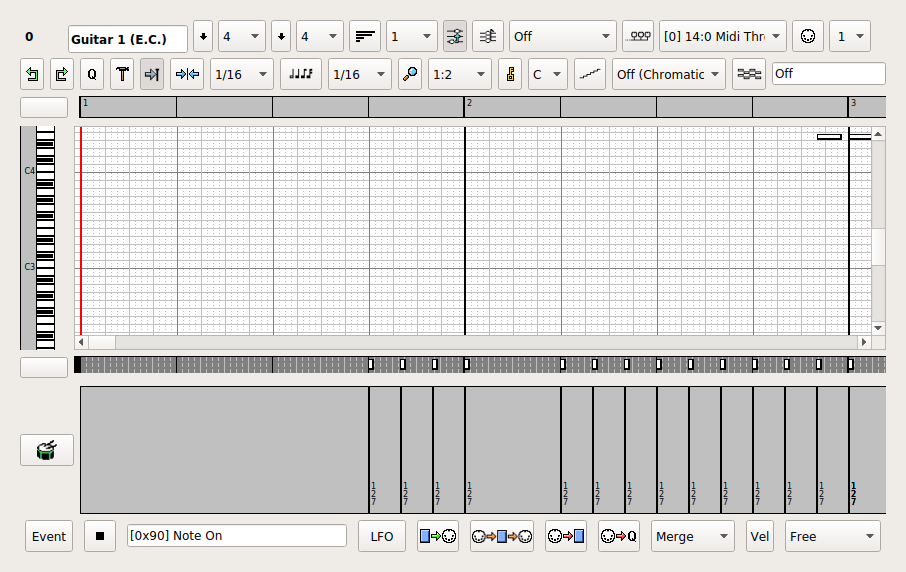
\includegraphics[scale=0.65]{roll.png}
   \caption{File / Options / Ext Keys (Condensed View)}
   \label{fig:seq66_menu_file_options_ext_keys}
\end{figure}

% Currently there is only one block of fields.  New blocks should also be
% marked by "itempar".

   \setcounter{ItemCounter}{0}      % Reset the ItemCounter for this list.

   \itempar{Ext Keys}{keyboard!extended keys}
   This block of fields in the \textbf{Options / Ext Keys} tab
   provides shortcut keys for more operations of \textsl{Sequencer66}, many of
   them ported from \textsl{Seq32} or \textsl{Kepler34}.

   \begin{enumber}
      \item \textbf{Song/Live toggle}.
      \item \textbf{Toggle JACK}.
      \item \textbf{Menu mode}.
      \item \textbf{Follow transport}.
      \item \textbf{Fast forward}.
      \item \textbf{Rewind}.
      \item \textbf{Pointer Position}.
      \item \textbf{Toggle mutes}.
      \item \textbf{Tap BPM}.
      \item \textbf{Song Record}.
      \item \textbf{One-shot Queue}.
         This new feature allows one-shot queuing of a pattern.
   \end{enumber}

   Most of these extended keys implement operations performed with button
   presses.  Some of the new keystrokes may not have a corresponding
   button.
   These values are saved as the \texttt{[extended-keys]} section of the "rc"
   configuration file.
%  However, not all builds of \textsl{Sequencer66} will
%  support the new keys.  Some of the new features can be enabled or disabled
%  during the build-configure step, and one's favorite Linux distro may decide to
%  disable some features.
%  An option might be disabled during the build process.
%  In this case, although the values will still be
%  stored in the "rc" file, they will be disabled or missing in this tab:

\begin{figure}[H]
   \centering 
%  \includegraphics[scale=0.65]{menu/menu_file_options_ext_keys_disabled.png}
   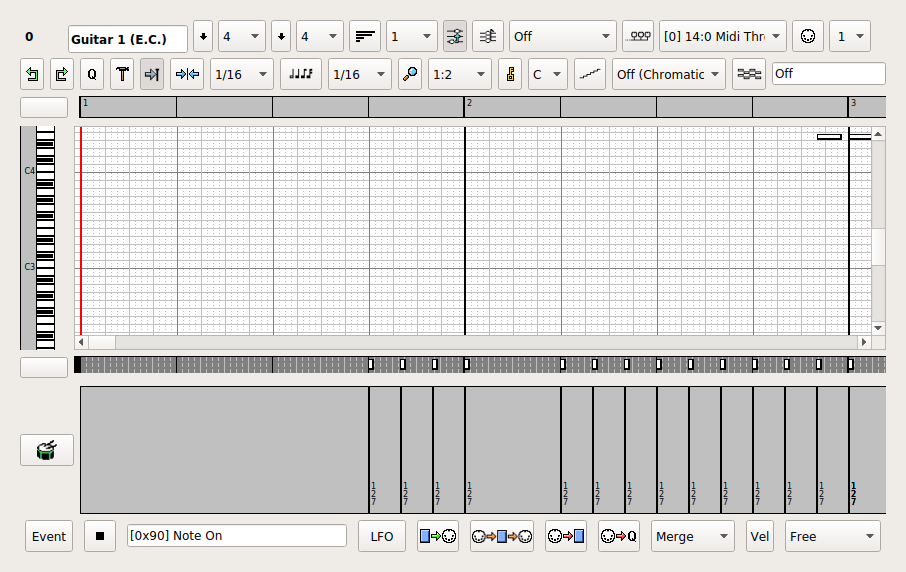
\includegraphics[scale=0.65]{roll.png}
   \caption{File / Options / Ext Keys (Disabled)}
   \label{fig:seq66_menu_file_options_ext_keys_disabled}
\end{figure}

   \index{song mode}
   Note the \textbf{Song/Live toggle} key.
   The \textsl{song mode} normally is in effect only when playback is started
   from the \textbf{Song Editor}.  Now this mode can be used from any
   window, if enabled by pressing this key.  There is also
   a button in the main window for this function, which shows the current state
   of this flag.  Note that this flag is also stored in the "rc" configuration
   file, as well as this hot-key value, which defaults to \texttt{F1}.

   \index{toggle JACK}
   \index{JACK toggle}
   The \textsl{JACK mode} is set via the
   \textbf{File / Options / JACK / JACK Connect} or 
   \textbf{JACK Disconnect} buttons.
%  But, if \textsl{Sequencer66} is built for
%  using the \textsl{Seq32} JACK support, then
   This keystroke will toggle between JACK connect and JACK disconnect.
%  Note that, with this kind of build,
   The \textbf{Song Editor} will also have a \textbf{JACK} button.
   The hot-key for this function defaults to \texttt{F2}.

   \index{menu mode}
   The \textsl{menu mode} indicates if the main menu of the
   main window is accessible or not.  It is disabled during playback
   so that more hot-keys can be used without triggering menu functions.
   It can also be disabled by the user; the default hot-key is \texttt{F3}.
   This feature is needed because the original \textsl{Seq24} had numerous
   conflicts between the menu key bindings and the default key bindings for the
   main window.

%  Here is Stazed's explanation of the feature, mildly edited:
%
%  \begin{quotation}
%     \textsl{"why disabling is needed when playing"}
%     The original seq24 had numerous conflicts between the menu key binding
%     and the default seq24 key binding for the mainwind sequence triggers.
%     For example: Ctrl-q (quits the program without prompt). If you place a
%     sequence in the default 'q' slot, you cannot use it with Ctrl-l or Ctrl-r
%     (default replace or queue) because the menu grabs the keys. Same goes for
%     the Alt-l or Alt-r (default snapshot 1 or 2). Try same as above with
%     Alt-f, Alt-v, Alt-h, Ctrl-n, Ctrl-o...  etc. So I just shut off all the
%     menus by default when playing because it seems that they should not be
%     needed then... especially in a live performance.
%
%     \textsl{"why a button?"}
%     On occasion I wanted to use the mainwnd key binding when stopped to set
%     the sequences to be ready before starting. It's also a sort of safety
%     feature as well, just toggle the menus off before going live so that you
%     don't hit Ctrl-q, Ctrl-n etc. forgetting things are not playing....
%  \end{quotation}

   \index{follow transport}
   \textsl{Follow transport} is a feature ported from \textsl{Seq32}.
   The default key is \texttt{F4}.
   It determines if \textsl{Sequencer66} follows JACK transport.

   \index{fast forward}
   \textsl{Fast forward} is a feature ported from \textsl{Seq32}.
   The default key is \texttt{F5}.
   While this key is held, the song pointer will fast-forward
   through the song.
   This feature does not have a corresponding button.
   This feature requires that the \textsl{Seq32} transport option be
   enabled at build time.

   \index{rewind}
   \textsl{Rewind} is a feature ported from \textsl{Seq32}.
   The default key is \texttt{F6}.
   While this key is held, the song pointer will rewind.
   This feature does not have a corresponding button.
   This feature requires that the \textsl{Seq32} transport option be
   enabled at build time (and now that is the default).
   Be sure not to use the following keys, which are already
   hardwired for other functions in the Pattern Editor and Song Editor:

   \begin{itemize}
      \item \texttt{p}.  Paint mode.
      \item \texttt{x}.  Escape paint mode.
   \end{itemize}

   \index{pointer position}
   \textsl{Pointer position} is a feature ported from \textsl{Seq32}.
   The default key is \texttt{F7}.
   When this key is pressed, the song pointer will move to the
   current position of the mouse, snapped.
   This feature does not have a corresponding button.

   \index{toggle mutes}
   \textsl{Toggle mutes} toggles the mute status of every
   pattern on every screen-set.  It corresponds to the
   \textbf{Edit / Toggle mute all tracks} or the 
   \textbf{Song / Toggle All Tracks}
   menu entries.  There is also a button in the main window for this function,
   which shows the current state of this flag.  Note that this
   hot-key value is stored in the "rc" configuration file, and
   defaults to \texttt{F8}.

   \index{tap bpm}
   \textsl{Tap bpm} allows the user to "tap" in time with some
   other music, and see the tap sequence translated into beats/minute (BPM).
   There is also a "0" button for this function.
   After 5 seconds, this feature resets automatically, so the user can try
   again if not satisfied.  At least two taps are needed for the
   BPM to be registered.

% VERIFY and the UNCOMMENT
%
%  Tap BPM causes events to be logged to the tempo track which is the first
%  track (track 0) by default.

\paragraph{Menu / File / Options / Mouse }
\label{paragraph:seq66_menu_file_options_mouse}

   This item selects the mouse-interaction method.

\begin{figure}[H]
   \centering 
%  \includegraphics[scale=0.65]{menu/menu_file_options_mouse_condensed.png}
   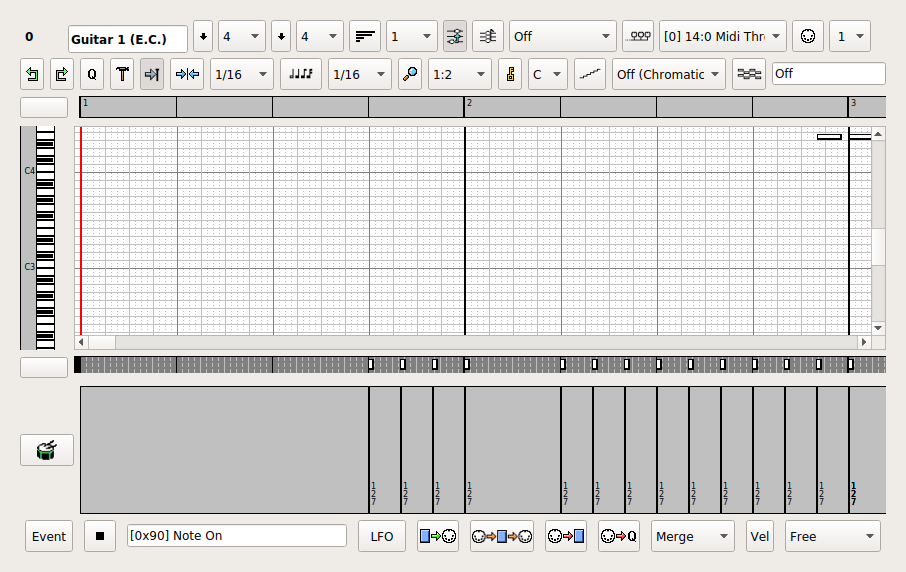
\includegraphics[scale=0.65]{roll.png}
   \caption{File / Options / Mouse (Condensed View)}
   \label{fig:seq66_menu_file_options_mouse}
\end{figure}

   \index{interaction method}
   \index{mouse interaction}
   \textbf{Interaction Method}

   The default mouse interaction method is \textbf{Seq24 (original style)}.
   The alternate mouse interaction method is \textbf{Fruity (similar to a
   certain well known sequencer)}.
   The "Fruity" interaction method
   is currently only available in the Gtkmm-2.4 user-interface, and it
   is not comprehensive.
   For Qt 5, only the original style is available, at this time.

   \index{mouse!fruity}
   The alternate method is presumably that of the \textsl{Fruity Loops}
   (now \textsl{FL Studio}) sequencer.  The fruity mode seems to involve the
   following rules:

   \begin{itemize}
      \item \textbf{Left-click left side}.
         Begin a grow/shrink operation for the left side.
         However, even in \textsl{Seq24}, this action is \textsl{broken}.
         It does allow one to move the note, however.
      \item \textbf{Left-click right side}.
         Begin a grow/shrink operation for the right side.
      \item \textbf{Left-click middle}.
         Move the object.  To clarify, each note image
         has an invisible "handle" on the left or the right side, with the
         middle providing a third area of interaction in the "fruity" mode.
      \item \textbf{Left-click}.
         Add an event if nothing selected.
      \item \textbf{Middle-click}.
         Split the note?
   \end{itemize}

   There may be a few more rules to add, when time allows.

% This paragraph needs to be moved to the pattern editor.

   The \textsl{Seq24} note-editing style is as expected for basic
   actions such as selecting and moving notes using the left mouse button.
   Drawing a note or event is a bit different, in that one must first
   \textsl{click and hold} the right mouse button, and then
   \textsl{click and drag} the right mouse button to insert notes,
   Notes are inserted to be at the current length and grid-snap values for
   the sequence editor for as long as the buttons are pressed.
   Notes are inserted only up to the specified sequence length.
   Once notes are inserted, moving the mouse with the left button still
   held down moves the notes to the new note value of the mouse.
   If one releases the left button, then presses and holds it again,
   more notes will be added in the same way.
   This is unconventional, but a powerful way to layer notes in a short
   sequence.
   We call it the
   \index{draw mode}
   \index{mode!draw}
   "draw mode" or
   \index{paint mode}
   \index{mode!paint}
   "paint mode".
   Drawing/painting can also be done while the sequence is playing,
   and notes will be added to be played the next time the progress bar crosses
   them.

%  \index{sequencer66 options}
%  The \textbf{Sequencer66 Options} section contains a couple of new options.

   \index{keys!Mod4}
   \index{mouse!Mod4}
   \label{new_mod4_mode}
   \textbf{Mod4 key preserves add (paint) mode in song and pattern editors}.
   In order to work with trackpads that don't permit simultaneous left
   and right clicks, the
   "Seq24" mode of mouse interaction can be modified in the
   Pattern or Song editors so that the Mod4 key (Super or Windows key)
   can be pressed when releasing the right mouse button.
   This keeps the mouse in note-add mode.
   Another right-click, without pressing Mod4, will exit this mode.

%  The reason for this feature is the crummy FocalTech touchpad on one of
%  the author's laptops.  This trackpad seems to have only a single button,
%  which the driver interprets as left or right depending where the finger
%  is when it is clicked.  There's no way to click the right and left
%  buttons at the same time.  There's no way to make a middle-click action.
%  What a crock!

   This option will not interfere with the Mod4 key being set
   in the \textbf{Keyboard} option tab, since the keys there mainly apply to
   the Patterns Panel (main window), not the pattern-editor window.

   \index{mouse!split mode}
   \label{new_split_mode}
   Middle click splits song triggers at nearest snap (instead of
   the halfway point).
% Move this section to the right place and simply create a section-reference to
% it here.

   \index{paint mode}
   Another way to turn on the paint mode has been added.
%  , based on a feature
%  found in a patch that someone posted about in some mailing list somewhere on
%  the internet.
   To turn on the paint mode, press the
   \index{keys!p}
   \texttt{p} key while in the sequence editor.
   This is just like pressing the right mouse button, but the draw/paint mode
   stays on.
   To get out of the paint mode, press the
   \index{keys!x}
   \texttt{x} key while in the sequence editor.
   These keys, however, do not work while the sequence is playing.

%  \index{todo:extend mouse support}
%  These convenience options are limited to the
%  pattern/sequence editor window and the performance editor window, and may
%  need some heavier testing.
   Note that some \textsl{Sequencer66} windows
   can use the ctrl-left-click as a middle click. 
 
\paragraph{Menu / File / Options / Jack Sync}
\label{paragraph:seq66_menu_file_options_jack_sync}

   This tab sets up JACK transport, if \textsl{Sequencer66}
   was built with JACK support.
%  It now also supports native JACK MIDI.
   This tab also sets up options for using LASH session management, \textsl{if}
   \textsl{Sequencer66} was built with LASH support, which is no longer the
   default, even though it is shown in the figure below.

\begin{figure}[H]
   \centering 
%  \includegraphics[scale=0.75]{menu/menu_file_options_jack_sync.png}
%  \includegraphics[scale=0.75]{new/menu_file_options_jack_sync.png}
%  \includegraphics[scale=0.65]{jack/menu_file_options_jack_sync.png}
   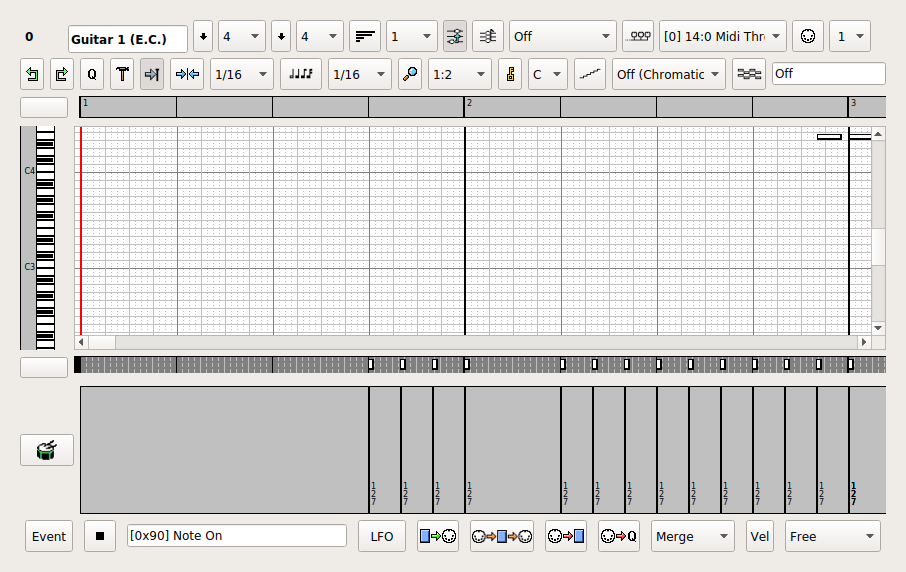
\includegraphics[scale=0.65]{roll.png}
   \caption{File / Options / JACK}
   \label{fig:seq66_menu_file_options_jack_sync}
\end{figure}

   The main sections in this dialog are:

   \begin{enumber}
      \item \textbf{JACK Transport/MIDI}
      \item \textbf{JACK Start Mode}
      \item \textbf{JACK Transport Connect and Disconnect}
      \item \textbf{LASH Options}
   \end{enumber}

   \setcounter{ItemCounter}{0}      % Reset the ItemCounter for this list.

   \itempar{Transport/MIDI}{jack sync!transport/midi}
   These settings are stored in the "rc" file settings group
   \texttt{[jack-transport]}.
   See \sectionref{subsec:seq66_rc_file_jack_transport},
   which describes this configuration option.
   This items collects the following settings:

   \begin{itemize}
      \item \textbf{Jack Transport}.
         \index{JACK!transport}
         Enables slave synchronization with JACK Transport.
         The command-line option is \texttt{--jack-transport}.
         The behavior of this mode of operation is perhaps not quite
         correct.  Even as a slave, \textsl{Sequencer66} can start and
         stop playback.
         Note that this option cannot be disabled via the mouse if the
         \textbf{Transport Master} option is enabled.  Disable that one first.
      \item \textbf{Transport Master}.
         \index{JACK!transport master}
         \textsl{Sequencer66} will attempt to serve as the JACK Master.
         The command-line option is \texttt{--jack-master}.
         \textbf{Tip}:
         \textsl{Sequencer66} generally works better as JACK Master.
         If this option is enabled the \textbf{JACK Transport} option is
         automatically enabled as well.
      \item \textbf{Master Conditional}.
         \index{JACK!master conditional}
         \textsl{Sequencer66} will fail to serve as the JACK Master if there is
         already a Master.
         The command-line option is \texttt{--jack-master-cond}.
         If this option is enabled the \textbf{JACK Transport} option is
         automatically enabled as well.
      \item \textbf{Native JACK MIDI}.
         \index{JACK!native midi}
         This option is for the \texttt{seq66} version of
         \textsl{Sequencer66}.
         If set, MIDI input and output use native JACK MIDI,
         rather than ALSA.  However, if JACK is not running on the
         system, then \texttt{seq66} will fall back to ALSA mode.
         The command-line option is \texttt{--jack-midi}.
   \end{itemize}

%  Note that there are long-standing issues with the JACK support of
%  \textsl{Seq24}, and \textsl{Sequencer66} currently inherits some of them,
%  in spite of some bug fixes.  Generally, if one experiences issues in
%  transport control, try making one of the other sequencer applications the
%  JACK Master.
%  If one starts \textsl{Sequencer66} in JACK mode without JACK running,
%  it will take a little while for \textsl{Sequencer66} to start up, and it
%  will fall back to ALSA usage.

   If one makes a change in the JACK transport settings, it is best to
   then press the \textbf{JACK Transport Disconnect} button, then the
   \textbf{JACK Transport Connect} button.  Another option is to restart
   \textsl{Sequencer66}... the settings are automatically saved when
   \textsl{Sequencer66} exits.

   \itempar{JACK Start mode}{jack sync!start mode}
   This item collects the following settings, also stored in the "rc" file
   settings group \texttt{[jack-transport]}.

   \begin{itemize}
      \item \textbf{Live Mode}.
         \index{JACK!live mode}
         \index{live mode}
         \index{non-playback mode}
         Playback will be in live mode.  Use this option to allow muting and
         unmuting of patterns.  This option might also be called "non-song
         mode".
         The command-line option is \texttt{--jack-start-mode 0}.
      \item \textbf{Song Mode}.
         \index{JACK!song mode}
         \index{song mode}
         \index{playback mode}
         \index{performance mode}
         Playback will use only the Song Editor's data.
         The command-line option is \texttt{--jack-start-mode 1}.
   \end{itemize}

   \textsl{Sequencer66} also selects the playback modes
   according to which window started the playback,
   reverting back to legacy \textsl{Seq24} behavior.
   \textsl{The main window}, or pattern
   window, causes playback to be in live mode.  The user can arm and mute
   patterns in the main window by clicking on sequences, using their hot-keys,
   and by using the group-mode and learn-mode features.
   The song editor causes playback to be in performance mode, also known as
   "playback mode", or \textbf{Song} mode.

   \itempar{Connect}{jack sync!connect}
   Connect to JACK Sync.
   This button is useful to restart JACK sync when making changes to it,
   or when \textsl{Sequencer66} was started in ALSA mode.

   \itempar{Disconnect}{jack sync!disconnect}
   Disconnect from JACK Sync.
   This button is useful to stop JACK sync when making changes to it.

   \itempar{LASH Options}{lash!option}
   Currently contains only one item, which enables the usage of LASH session
   management.  Currently, \textsl{Sequencer66} needs to be restarted to
   complete the enabling or disabling of LASH support.  Like the rest of the
   options, this one is written to the "rc" configuration file.
   However, LASH is no longer supported in the default build.

   Finally, there is a new button (labelled \textsl{Master} in the following
   figure) in the main window to bring up directly the
   \textbf{JACK} (or \textbf{JACK/LASH}) page.

\begin{figure}[H]
   \centering 
%  \includegraphics[scale=0.75]{menu/menu_file_options_jack_sync.png}
%  \includegraphics[scale=0.65]{new/main_master_button.png}
   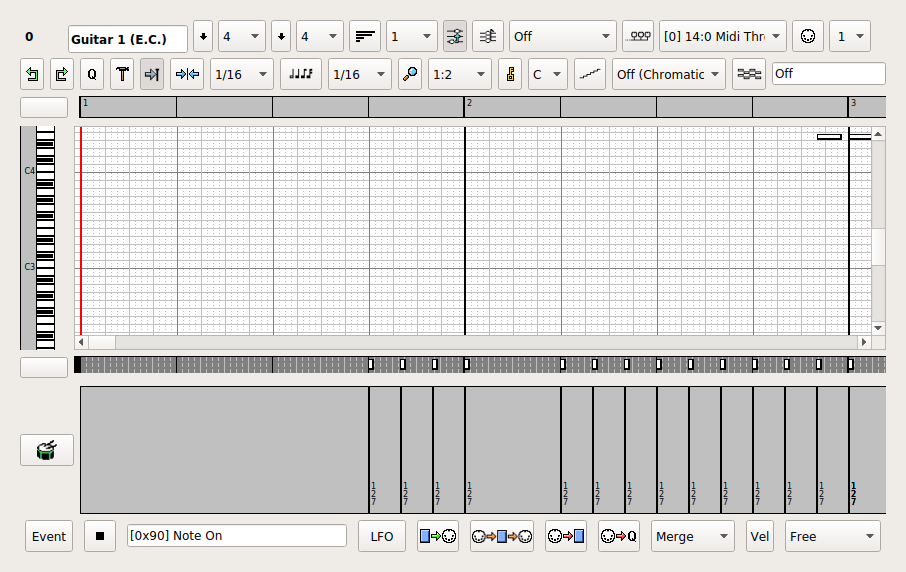
\includegraphics[scale=0.65]{roll.png}
   \caption{JACK Connection Button}
   \label{fig:seq66_main_master_button}
\end{figure}

   This button not only brings up the JACK page, but also shows the current
   status of the MIDI connection:
   \textbf{Master} (JACK Transport Master),
   \textbf{Slave} (JACK Transport Slave),
   \textbf{JACK} (native JACK MIDI, overrides any transport label),
   and \textbf{ALSA} (overridden by any transport label).
   \index{jack page!ctrl-p}
   \index{keys!ctrl-p}
   The \texttt{Ctrl-P} key will also bring up this page.

   One thing to note is that, while playing, the JACK/ALSA button is disabled.
   However, one can still get to the JACK options via the main File menu.
   JACK connection and disconnection are disabled during playback, but the
   buttons don't yet reflect that status.

\subsection{Menu / Edit}
\label{subsec:seq66_menu_edit}

   The \textbf{Edit} menu has undergone some expansion lately.

\begin{figure}[H]
   \centering 
%  \includegraphics[scale=0.65]{new/menu_edit_0_90.png}
   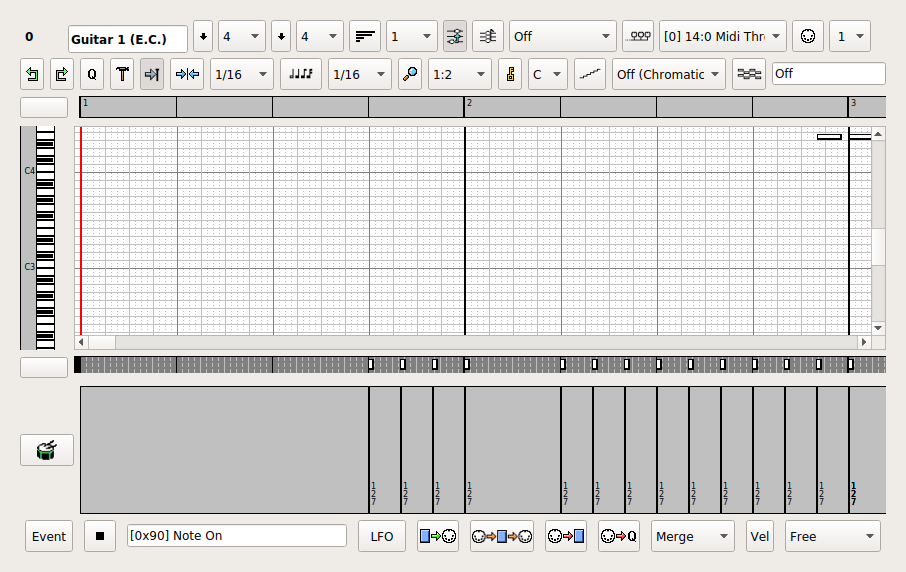
\includegraphics[scale=0.65]{roll.png}
   \caption{Edit Menu}
   \label{fig:seq66_menu_edit_0_90}
\end{figure}

   \begin{enumber}
      \item \textbf{Preferences...} (only in the Qt user-interface)
      \item \textbf{Song Editor...}
      \item \textbf{Apply song transpose}
      \item \textbf{Clear mute groups}
      \item \textbf{Reload mute groups}
      \item \textbf{Mute all tracks}
      \item \textbf{Unute all tracks}
      \item \textbf{Toggle mute all tracks}
   \end{enumber}

   \setcounter{ItemCounter}{0}      % Reset the ItemCounter for this list.

   \itempar{Preferences}{edit!preferences}
   In the Qt user-interface, there is a \textbf{Preferences} menu entry,
   corresponding to the Gtkmm user-interface's \textbf{File / Options}
   menu entry.

   \itempar{Song Editor}{edit!song editor}
   \index{song editor}
   This item is the same as the 
   \textbf{View / Song Editor toggle} menu entry.  It toggles the presence of
   the main song editor.

   \itempar{Apply song transpose}{edit!song transpose}
   \index{song transpose}
   Selecting this item applies the song transposition value to
   \textbf{all} sequences/patterns that are marked as transposable.
   (Normally, drum tracks are \textsl{not} transposable).
   This actively changes the note/pitch value of all note and aftertouch events
   in the pattern.
%  Once the transpositions are done, the transposition value is set to 0.
   For the setting of song transpose, see
   \sectionref{sec:seq66_song_editor}, for more information.
   Also note that transpose can be enabled in the patterns panel for each
   pattern (see \sectionref{subsubsec:seq66_patterns_pattern_filled}) and
   in the sequence editor
   (see \sectionref{sec:seq66_pattern_editor}).

   \itempar{Clear mute groups}{edit!clear mute groups}
   \index{mute groups}
   A feature of \textsl{Seq24} and \textsl{Sequencer66} is that the mute groups
   are saved in both the "rc" file
   (see \sectionref{subsec:seq66_rc_file_mute_group})
   \textsl{and} in the "MIDI" file
   (see \sectionref{subsec:legacy_midi_format}).

   This menu entry clears them. If this resulted in any mute-group sequences
   status being set to false, then the user is prompted to save the MIDI
   file, so that it will no longer have any
   mute-group information.  And then, if the
   application exits, the cleared mute-group information is also saved to
   the "rc" file.
%  We'd like to be able to handle the "rc" and "MIDI"
%  mute-groups separately in the future.

   \itempar{Reload mute groups}{edit!load mute groups}
   \index{rc!mute groups}
   This menu entry reloads the mute-groups from the "rc" file.
   So, if one loads a MIDI file that has its own mute groups that one does not
   like, this command will restore one's favorite mute-grouping from the "rc"
   file.

   \itempar{Mute all tracks}{edit!mute all tracks}
   \index{mute all}
   This menu entry, available only in \textbf{Live} mode,
   immediately mutes \textsl{all} patterns in the entire song.

   \itempar{Unmute all tracks}{edit!unmute all tracks}
   \index{unmute all}
   This menu entry, available only in \textbf{Live} mode,
   immediately unmutes \textsl{all} patterns in the entire song.

   \itempar{Toggle mute all tracks}{edit!toggle all tracks}
   \index{toggle mute all}
   This option toggles the mute/armed status of \textbf{all} tracks.
   It is only available in \textbf{Live} mode, which overrides \textbf{Song}
   mode even if the Song Editor is focussed.
   \textsl{Do not confuse it with the main \textbf{Mute} button, which toggles the
   status only of the tracks that are armed and remembers them.}

\subsection{Menu / View}
\label{subsec:seq66_menu_view}

   If the "allow two perfedits" option is turned off in the "user"
   configuration file, this menu item has only one entry, \textbf{Song Editor}, 
   which is already covered by a button at the bottom of the Patterns
   window.  Selecting this item bring up the Song Editor window.
   See \figureref{fig:song_editor_window}.
   The Song Editor window can also be brought up via the
   \index{song editor!ctrl-e}
   \index{keys!ctrl-e}
   Ctrl-E key.

   If the \textbf{allow two perfedits} option is turned on in the "user"
   configuration file, this menu item has two entries,
   as shown in the following figure:

\begin{figure}[H]
   \centering 
%  \includegraphics[scale=0.65]{menu/menu_view-dual-song-editors.png}
   \includegraphics[scale=0.65]{roll.png}
   \caption{Dual Song Editor Entries in View Menu}
   \label{fig:seq66_menu_view_song_editors}
\end{figure}

   Note that only the first Song Editor has a user-interface button and
   a hot-key.  Also note that there can be issues bringing up the second
   song-editor with the hot-key.  The menu entry will always work.
   If two song editors are up, they each track any changes made in the other
   song editor.  But the main purpose of two song editors is to arrange two
   different parts of the performance at the same time when not all the
   patterns will fit in one window.

   In the Qt user-interface, there is a \textbf{Song} tab in the main window.
   But there is also song-editor button in the main window
   and a menu entry in \textbf{Edit / Song Editor},
   which bring up a separate window for the song-editor.
   Do not try to use both windows for song-editing at the same time; they
   are not synchronized.

\subsection{Menu / Help / About...}
\label{subsec:seq66_menu_about}

   This menu entry shows the "About" dialog.

\begin{figure}[H]
   \centering 
%  \includegraphics[scale=0.75]{menu/menu_help_about.png}
%  \includegraphics[scale=0.65]{new/menu_help_about.png}
   \includegraphics[scale=0.65]{roll.png}
   \caption{Help / About}
   \label{fig:seq66_menu_help_about}
\end{figure}

   The Qt version is slightly different.
%  That dialog provides access to the credits for the program, including the
%  authors and the project documentors.  It has recently been updated
%  to show Git version-control information as well.

\begin{figure}[H]
   \centering 
%  \includegraphics[scale=0.65]{menu/menu_help_credits.png}
   \includegraphics[scale=0.65]{roll.png}
   \caption{Help Credits}
   \label{fig:seq66_menu_help_credits}
\end{figure}

   Shows who has worked on the program, with the original author at the top
   of the list.

\begin{figure}[H]
   \centering 
%  \includegraphics[scale=0.65]{menu/menu_help_doc.png}
   \includegraphics[scale=0.65]{roll.png}
   \caption{Help Documentation}
   \label{fig:seq66_menu_help_doc}
\end{figure}

   Shows who has documented this project.

\subsection{Menu / Help / Build Info...}
\label{subsec:seq66_menu_build_info}

   This menu entry shows the "Build Info" dialog.  This list of
   build options enabled in the current application is the same list
   that it generated via this command line:

   \begin{verbatim}
      $ seq66 --version
   \end{verbatim}

\begin{figure}[H]
   \centering 
%  \includegraphics[scale=0.50]{new/menu_help_build_info.png}
   \includegraphics[scale=0.65]{roll.png}
   \caption{Help / Build Info}
   \label{fig:seq66_menu_help_build_info}
\end{figure}

%-------------------------------------------------------------------------------
% vim: ts=3 sw=3 et ft=tex
%-------------------------------------------------------------------------------


% Patterns Panel

%-------------------------------------------------------------------------------
% seq66_patterns_panel
%-------------------------------------------------------------------------------
%
% \file        seq66_patterns_panel.tex
% \library     Documents
% \author      Chris Ahlstrom
% \date        2015-08-31
% \update      2018-10-27
% \version     $Revision$
% \license     $XPC_GPL_LICENSE$
%
%     Provides the concepts.
%
%-------------------------------------------------------------------------------

\section{Patterns Panel}
\label{sec:seq66_patterns_panel}

   \textsl{Seq66} works with patterns (loops, tracks, or
   sequences) that are repeated throughout a song.
   One composes and edits small patterns,
   and combines them to create a full song.  This is a powerful way
   to work, and makes one productive within an hour.

   The \textsl{Seq66 Patterns Panel} is the
   \index{main window}
   \textbf{main window} of \textsl{Seq66}.
   See \figureref{fig:seq66_main_screen}.
   It is called the "main window" or the "patterns window".
   It is here one creates a set of patterns
   (see \sectionref{subsubsec:concepts_terms_screen_set}),
   manages the configuration, controls the playback rate, adds tempo events,
   and opens the pattern, song, event, or playlist editors.

   \index{live mode}
   \index{mode!live}
   \index{mode!song}
   When the Patterns Panel has the application focus,
   and \textsl{Seq66} is \textsl{not} running in \textbf{Song} mode,
   it puts \textsl{Seq66} in \textbf{Live} mode.
   The musician can
   control the playback and muting/unmuting of each pattern in
   the song, while it is playing, from within this window.

   \index{song mode}
   \index{mode!song}
   If the song editor (see \sectionref{sec:seq66_song_editor})
   has the input focus, it controls the muting/unmuting of
   each pattern, and \textsl{Seq66} runs in \textbf{Song} mode.
   (There are ways to override this behavior.)

%  However, if \textsl{Seq66} is using JACK transport, then, instead of
%  the behavior described above, live versus song mode is controlled by the
%  JACK start mode option (see the \textbf{JACK Start mode} item in
%  \sectionref{paragraph:seq66_menu_file_options_jack_sync}).

   For exposition, we break the Patterns Panel
   into a menu bar, a top panel, a pattern panel, and a bottom panel.
   The \textsl{Seq66} menu bar is discussed in
   \sectionref{sec:seq66_menu}.
   The Qt and Gtkmm user-interfaces differ in the arrangement of buttons and
   panels; and the Qt interface uses tabs.

\subsection{Patterns / Top Panel}
\label{subsec:seq66_patterns_panel_top}

   The top panel of the Pattern window is simple, consisting of the
   name of the program and a few controls.  The latest version adds more
   buttons.
   
%  The original version looked like
%  this:

% \begin{figure}[H]
%    \centering 
%    \includegraphics[scale=0.75]{pattern-window-top-panel-items.png}
%    \caption{Patterns Panel, Top Panel, Older Version}
%    \label{fig:pattern_window_top_panel_items}
% \end{figure}

%  But, if compiled with \texttt{SEQ66\_STAZED\_MENU\_BUTTONS} defined,
%  there are some extra buttons available:

\begin{figure}[H]
   \centering 
%  \includegraphics[scale=0.50]{pattern-window-top-panel-items-new.png}
%  \includegraphics[scale=0.50]{new/pattern-window-top-panel-items-new.png}
%  \includegraphics[scale=0.50]{new/pattern-window-top-panel.png}
%  \includegraphics[scale=0.75]{new/pattern-window-top-panel.png}
   \includegraphics[scale=0.65]{roll.png}
   \caption{Patterns Panel, New Top Panel Items}
   \label{fig:pattern_window_new_top_panel_items}
\end{figure}

   This figure shows the appearance of the main window top panel.
   These items appear in the Gtkmm-2.5 user-interface.
   The Qt user-interface is arranged differently, but has roughly the
   same functionality.
   See \figureref{fig:seq66_main_screen_qt}.

%  If \textsl{Seq66} was built with
%  \texttt{SEQ66\_MENU\_BUTTON\_PIXMAPS} defined, then the buttons have icons
%  on them; otherwise they have text.  The figure shows what they look like,
%  and how they look with the song/live and toggle-menu functions activated.
 
   \begin{enumber}
      \item \textbf{Song/Live}
      \item \textbf{Toggle Playing Tracks}
      \item \textbf{Toggle Menu}
      \item \textbf{ALSA/JACK Modes}
      \item \textbf{Song Progress Bar}
      \item \textbf{Time Display Selection}
      \item \textbf{Mute Group Learn}
   \end{enumber}

   \setcounter{ItemCounter}{0}      % Reset the ItemCounter for this list.

   \itempar{Song/Live}{pattern!song/live}
   \index{pattern!song/live}
   This new button allows the Song mode to be in force even if
   the \textbf{Song Editor} does not have the focus of the application.
   However, if the \textbf{Song Editor} does have focus, it overrides this
   button, to preserve expected behavior.
   There is also a configurable hot-key associated with it,
   which defaults to \texttt{F1}, and is configurable in the "rc" file and
   the \textbf{File / Options / Ext Keys} page.

   \itempar{Toggle Tracks}{pattern!toggle tracks}
   \index{pattern!toggle tracks}
   This button changes the status of all of the
   \textsl{playing} tracks, reversing the
   mute status of each pattern that is playing.
   The next click will then unmute only those tracks.
   Because it can be confusing, this button is disabled (not shown
   in the figure) in Song mode.
   There is also a configurable hot-key associated with it, called
   \textbf{Toggle mutes},
   which defaults to \texttt{F8}, and is configurable in the "rc" file and
   the \textbf{File / Options / Ext Keys} page.

   \itempar{Toggle Menu}{pattern!toggle menu}
   \index{pattern!toggle menu}
   This button enables and disables the main menu.
   Disabling it allows additional hot-keys to be configured,
   without calling forth menu entries by accident.
   There is also a configurable hot-key associated with this toggle, called
   \textbf{Menu mode},
   which defaults to \texttt{F3}, and is configurable in the "rc" file and
   the \textbf{File / Options / Ext Keys} page.

   \itempar{ALSA/JACK Modes}{pattern!ALSA/JACK modes}
   \index{pattern!ALSA/JACK mode}
   This button sets the ALSA versus
   JACK modes, including JACK transport and native JACK MIDI playback and
   recording.
   When clicked, it brings up the JACK connection page from the
   \textbf{File / Options} dialog.  The hot-key for this button
   is \texttt{Ctrl-P}.

   \itempar{Song Progress Bar}{pattern!progress bar}
   \index{pattern!progress}
   \index{pattern!"main time"}
   The \textbf{Song Progress Bar} is also known as the "main time" bar.
   Also included is a numeric representation of the "BBT" (bar:beat:ticks).
   In the Gtkmm-2.4 user-interface,
   this bar shows a number of small black cursors ("pills") that show the
   progress of the song through the various patterns.  For short patterns,
   the progress is fast.  For patterns that last longer, the progress is
   slow.  The whole field flashes in time with the beat.
   This field shows that something is going on.  It can also indicate
   the relative lengths of the various patterns.
   In the Qt user-interface, this bar is shown as four boxes
   which blink in time with playback.
 
   Note that the individual pattern boxes in the main panel, for
   patterns that are not empty, have their own
   moving progress cursor, a vertical line in each box.
   By default, this progress line is black, but it can be changed to
   other colors via a "user" configuration file entry in the 
   \texttt{[user-interface-settings]} section.
   Set the \texttt{progress\_bar\_colored} item to a value ranging from 0
   (black) to 6 (dark cyan).
   There is also a \texttt{progress\_bar\_thick} item to enable a thicker
   progress bar, for better visibility.

%  Even if not enabled, the currently-selected pattern will show as highlighted
%  in dark-cyan.

   \itempar{Time Display Selection}{pattern!time display}
   The \textbf{Time Display Selection} is also known as the "main time" bar.
   This button toggles between the states of \textbf{BBT} (bar:beats:ticks)
   and \textbf{HMS} (hours:minutes:seconds).

   \itempar{Mute Group Learn}{pattern!mute group learn}
   \index{L button}
   \index{"L" button}
   This button is also known as the "L" button.
   Click this button, and then press a mute-group key
   to store the mute-state (whether armed or unarmed)
   of all the patterns with in that key.
   In addition to this button, one can also press
   the \texttt{Ctrl-L} key.
%  (analogous to the \texttt{Ctrl-E}
%  keystroke that brings up the Song Editor).
   \index{auto-shift}
   \index{group-learn!auto-shift}
   \index{shift-lock}
   \index{group-learn!shift-lock}
   When in group-learn mode, the \texttt{Shift} key cannot be hit, so the
   group-learn mode automatically converts the keys to their shifted versions.
   This feature known as \textsl{shift-lock} or \textsl{auto-shift}.

   See the \textbf{File / Options / Keyboard} menu entry for the
   dialog showing the available mute-group keys and the corresponding
   hot-key for the "L" button.
   This key is usually the \texttt{Insert} key.  Unlike the button or the
   \texttt{Ctrl-L} key, this key must be held down while pressing the desired
   mute-group key.
   This is a clumsy thing on our main keyboard... one must press and hold
   \texttt{Shift-Fn-Insert} to get the \texttt{Insert} key, and then also
   press the desired mute-group key.  A real knuckle-buster!
   We have our own alternate setup (stored in the file
   \texttt{sequencer66.rc.example}.
   And we've also added the "shift-lock" feature for this reason.

   Group-learn is a modifier key to be pressed
%  \textsl{together} with
   just before pressing
   the desired group key, and the group on/off keys are there to enable
   each group, \textsl{not} to toggle group states.

   To set up the mute groups, press the 'L' button, and then press a key on
   the keyboard to 'learn' or 'save' the preset. Looking at the list of keys
   assigned for these mute groups (in \textbf{File / Options / Keyboard}),
   the first bank of keys are "!", "'", "?", etc., and the second bank are
   "Q", "W" "E", etc.
%  Note that these shifted keys do not toggle patterns, but
%  set them to a saved mute-group of armed and unarmed patterns.
   If the key is valid, then the following prompt occurs:

\begin{figure}[H]
   \centering 
%  \includegraphics[scale=0.65]{pattern-window-group-learn-confirmation.png}
   \includegraphics[scale=0.65]{roll.png}
   \caption{Group Learn Confirmation Prompt}
   \label{fig:pattern_window_group_learn_confirmation}
\end{figure}
   
   When you ask the program to 'learn' the key, one cannot
   use the Shift key, so one normally could not use the "!" or
   other symbol keys.
   In fact, the process stops as soon as the Shift key is pressed:

\begin{figure}[H]
   \centering 
%  \includegraphics[scale=0.65]{pattern-window-group-learn-failure.png}
   \includegraphics[scale=0.65]{roll.png}
   \caption{Group Learn Failure Prompt (Shift Key)}
   \label{fig:pattern_window_group_learn_failure}
\end{figure}

   \index{caps lock in learn mode}
   \index{auto-shift}
   \index{group-learn!auto-shift}
   \index{shift-lock}
   \index{group-learn!shift-lock}
   To avoid this issue with the \texttt{Shift} key, \textsl{Seq66} now
   "shift-locks" the keys while group-learn is in progress, so
   that none of the keys, whether letters or the punctuation characters above
   the numbers, need the \texttt{Shift} key to be held, to learn them.
   Thus, there is now no need to use the \textbf{Caps Lock} is \textsl{On} before
   starting the "learn" process.  We tend to map the
   \texttt{Caps Lock} key as the \textsl{true} Control key, so that
   \texttt{Caps Lock} is no longer available anyway
   (it is one of the most useless keys \textsl{ever}).

   Remember, though, that once learned, the \texttt{Shift} is then
   needed to call up the mute-group that was learned.

   There is another way for mute-group learn to fail.
   With the recent ability of \textsl{Seq66} to increase the set size via
   the \texttt{--option sets=8x12} (for example), there can be fewer than 32
   mute-groups available.   This can be seen by viewing
   \textbf{File / Options / Keyboard} when larger set-sizes are in force:

\begin{figure}[H]
   \centering 
%  \includegraphics[scale=0.75]{group-learn-limited.png}
   \includegraphics[scale=0.65]{roll.png}
   \caption{Group Learn Keys With Larger Set Size}
   \label{fig:pattern_window_group_learn_limited}
\end{figure}

   Note that only 10 mute-groups (0 to 9) are available with an 8x12 set size.
   Groups 10 and above are not available, and this is indicated by the word
   "Clear".  Don't worry, though, all of the mute-group key settings still
   exist, and are still present in the "rc" configuration file in the
   \texttt{[keyboard-group]} section.

   But when one attempts a group-learn using one of the unavailable keys,
   an error occurs, as shown in the following prompt.

\begin{figure}[H]
   \centering 
%  \includegraphics[scale=0.75]{pattern-window-group-learn-limit.png}
   \includegraphics[scale=0.65]{roll.png}
   \caption{Group Learn Limit Prompt}
   \label{fig:pattern_window_group_learn_limit}
\end{figure}

   This prompt also appears if one tries to use the shifted version of an
   unavailable mute-group key to toggle patterns; this makes it obvious what
   has gone wrong.

   \textsl{
   At some point in the future, we may allow a much larger number of sets, so
   that all 32 mute-groups are always available.  We have to think hard about
   that enhancement, however.
   }

   One can configure the MIDI settings in similar ways
   by assigning MIDI commands to arm or toggle loops, using 
   \index{rc file}
   the 'on' option in the "rc" file.
   See \sectionref{subsec:seq66_rc_file_midi_control}.

%  The mute group doesn't toggle... it turns on.
%  \index{group!toggle}
%  \index{group!arm}
%  \index{group!unmute}
%  One can toggle the playing status of up to 32 previously
%  One can set the playing status of up to 32 previously
%  defined mute/unmute patterns (groups) in the active screenset, similar to
%  hardware sequencers.  One can mute-unmute (according to the group
%  definition) all loops in the playing screenset, which is the only one that
%  can have sequences playing if a mute group is selected
%  (like a live sequencer).
%
%  This arming is done either by one of the \textsl{group arm} keys
%  or by a MIDI controller, both assigned in the
%  \index{rc file}
%  \texttt{~/.config/sequencer66/sequencer66.rc} or \texttt{~/.seq24rc} files,
%  and easily modified in the \textbf{File / Options / Keyboard} tab.
%  These characters can be shown in each pattern (and in 0.9.11 and above, no
%  matter which screenset is active).
%
%  A mute/unmute pattern (group) is stored by holding a
%  \index{group!learn}
%  \textsl{group learn} key (\texttt{Insert} by default) while pressing the
%  corresponding \textsl{group arm} key.  The "L" button can also be used to
%  enter "Learn" mode.
%  Once a learn-key is pressed, the set of muted/unmuted patterns in the
%  current set is memorized, and can be recalled later.

%  There are also keys assigned to turn on/off the group functionality.

%  Once learned, the "Shifted" version of the keyboard keys can be
%  used to select a learned group.

   Remember that groups work with the playing ("in-view") screen-set.
   One must change the screenset and give it the command to make it the
   playing one.
   \index{keys!Home}
   By default, the \texttt{Home} key is configured for this purpose.

   So, for example, if one sets \texttt{A} to turn on the
   patterns in slots 1 and 2 in set 0 (the first set), then pressing
   \texttt{A} in another set will arm the patterns in the same relative
   location in the current set.
   This setup is flexible, but takes some thought.
   One can set up a number of mute-groups, and decide to use them
   for all sets, or mentally allocate one mute-group per set.
   Please note that a mute-group key does not \textsl{toggle} the saved
   armed patterns... it can only turn them on.

%  \index{rc file}
%  It is all configurable in the "rc" file.

   Let's go through an example using the \texttt{Home} key (or whatever key is
   configured as the \textbf{Set Playing Screenset} key.)

   \begin{enumber}
      \item Load a song with more than one screen-set.
      \item Unmute the pattern(s) in the first set and start playback.
      \item Use the "\texttt{]}" (\textbf{Screenset Up}) key to move to the next
         set.  Note that the first set is still playing.  Also note that the
         now-current set is \textsl{not} playing.
      \item Press the \texttt{Home} key.
         Note that the first set turns off, and the current set turns on.
         These steps can be repeated at will.
      \item Finally, hit the \texttt{F8} (\textbf{Toggle Mutes}) key.
         Note that all tracks on all sets toggle muting each time this key is
         pressed.
   \end{enumber}

\subsection{Patterns / Main Panel}
\label{subsec:seq66_patterns_panel_main}

   The main panel of the Patterns window provides a grid of empty boxes,
   each box delimited by brace-like lines at left and right.
   Each filled box represents a loop or pattern.
   One sees only 32 loops at a time in the main panel (but many more than
   32 loops can be supported by \textsl{Seq66}).
   \index{screen-set}
   This group of 32 loops is called a "screen-set", as discussed in
   \sectionref{subsubsec:concepts_terms_screen_set}.
   One can switch between sets by using the
   \index{keys![}
   \index{keys!screenset down}
   "\texttt{[}" and
   \index{keys!]}
   \index{keys!screenset up}
   "\texttt{]}" keys on the keyboard, or by using
   the spin-widget-driven, labelled \textbf{Set} interface item, or
   \index{keys!Home}
   \index{keys!screenset play}
   by hitting the (default) \texttt{Home} key to make it the playing screenset,
   or by hitting \texttt{Page-Up} or \texttt{Page-Down} with the pattern window
   in keyboard focus.
   There are a total of 32 sets, for a total of 1024 loops/patterns. 
   Only one screen-set can be controlled at a time, in general.
%  have found; have not yet tried to verify this assertion.
   But any number of screensets can be playing at the same time.

   Note that the \texttt{Page Up} and \texttt{Page Down} keystrokes, and their
   counterparts in
   \textbf{File / Options / Keyboard / Control Keys / Screenset Up}
   and \textbf{Screenset Down}, can be used in lieu of the
   \textbf{Set} spin-button.

   It is important to note that keystroke control of the screen-set will
   wrap-around in screen-set values (i.e. screen-set down at 0 results in
   screen-set 31, and screen-set up at 31 results in screen-set 0).
   However, the spinbuttons will stop up at 31 and stop down at 0.
   We consider this a feature rather than a bug, at this time.

\begin{figure}[H]
   \centering 
%  \includegraphics[scale=0.75]{pattern-window-main-panel-items.png}
   \includegraphics[scale=0.65]{roll.png}
   \caption{Patterns Panel, Main Panel Items}
   \label{fig:pattern_window_main_panel_items}
\end{figure}

   The individual items annoted in this figure are described in
   \sectionref{subsubsec:seq66_patterns_pattern_filled}, in more detail.
   The slot at the bottom left of this figure shows some new features:

   \begin{itemize}
      \item The sequence number appears at the bottom left of the slot.
      \item The buss number (re 0) and the channel number (re 1) appears
         to the right of the sequence number, in the format "0-1".
      \item To the right of that, the time signature ("4/4") appears, at the
         bottom.
      \item The hot-key for muting/unmuting the pattern appears next,
         at the bottom right of the slot.
      \item The title of the sequence appears at the top left of the pattern
         slot.
      \item The length of the sequence, in number of measures (bars), appears
         at the upper right of the slot.
      \item Notice the default alternate font, which has a little more body
         than the \textsl{Seq24} font.
   \end{itemize}

   Observe that feature in the first figure of the next section.
   The two main items are the empty \textsl{pattern slot}, and the slot filled
   with a MIDI \textsl{pattern}:

   \begin{enumber}
      \item \textbf{Pattern Slot}
      \item \textbf{Pattern}
   \end{enumber}

\subsubsection{Pattern Slot}
\label{subsubsec:seq66_patterns_pattern_slot}

   \index{pattern!slot}
   An empty box is a slot for a pattern.
   If a pattern is present in the slot, the top line will show
   the title of the pattern, and the number of measures in the pattern.
   The latter is not shown on some of the figures in this manual, a
   lack we will ave to rectify someday.
   Also, these colors are not yet supported in the Qt user-interface.

   A pattern can show a number of different statuses based on the coloring
   of elements in the pattern slot. 

\begin{figure}[H]
   \centering 
%  \includegraphics[scale=0.75]{new/slots.png}
   \includegraphics[scale=0.65]{roll.png}
   \caption{Various Status of Pattern Slots}
   \label{fig:pattern_slots_statuses}
\end{figure}

   Not shown in the figure are the gray pattern
   colors resulting from queuing and one-shot queuing, nor is the
   number-of-measures number shown.
   The colors have meaning (in the Gtkmm user-interface only):

   \begin{itemize}
      \item \textbf{Empty background}.  Whether the classic gray pattern
         of \textsl{Seq24}, or the many patterns of \textsl{Seq66},
         including all black with yellow sequence numbers, this
         slot coloring indicates that the slot is unused.
      \item \textbf{White background}.  Unarmed (muted) patterns show black
         text on a white background.
      \item \textbf{Black background}.  Armed (unmuted) pattern.  If the text
         is yellow, it is a pattern with no MIDI events, but is armed.  Note
         that armed/unmuted patterns can be exported if they have a layout in
         the Song Editor.
      \item \textbf{Yellow background}.  A pattern with no MIDI events, just
         textual MIDI information.  If armed (uselessly), it is yellow text on
         a black background (not shown).
      \item \textbf{Cyan background, black text}.
         An unarmed pattern currently being edited in a 
         \textbf{Pattern Editor} or event
         editor. Or, if an SMF 0 MIDI file was just opened or imported, this
         color combination indicates the SMF 0 format track with all of the
         data in the song, which only occurs in slot 16 (unless the user then
         dragged it to another slot).
      \item \textbf{Black background, cyan text}.
         An armed pattern currently being edited in a 
         \textbf{Pattern Editor} or event
         editor.  Or an armed SMF 0 format MIDI sequence.
      \item \textbf{Red events}.
         Indicates a pattern for which the new transpose feature is
         disabled.  The white, black, and cyan background have the same
         meanings as in the other items for statuses of unarmed, armed, and
         currently being edited.
   \end{itemize}

   As of version 0.95, the user can also apply coloring to each sequence.
   This feature was adopted from \textsl{Kepler34} (\cite{kepler34}).
   Here is the new pattern menu for sequence color:
   \index{pattern!color menu}

\begin{figure}[H]
   \centering 
%  \includegraphics[scale=0.75]{new/seq66-sequence-color-menu.png}
   \includegraphics[scale=0.65]{roll.png}
   \caption{Sequence/Pattern Color Menu}
   \label{fig:pattern_window_sequence_color_menu}
\end{figure}

   Here is a sample of the coloration as it appears in the patterns panel and
   in the song editor:
   \index{pattern!coloring}

\begin{figure}[H]
   \centering 
%  \includegraphics[scale=0.75]{new/seq66-sequence-coloration.png}
   \includegraphics[scale=0.65]{roll.png}
   \caption{Sequence/Pattern Coloration}
   \label{fig:pattern_window_sequence_coloration}
\end{figure}

   \index{pattern!right click}
   \index{slot!empty slot right-click}
   Right-click on an empty box one brings up a menu to create
   a new loop, as well as some other operations:

\begin{figure}[H]
   \centering 
%  \includegraphics[scale=0.75]{pattern/pattern-empty-right-click-menu.png}
%  \includegraphics[scale=0.65]{new/pattern-empty-right-click-menu.png}
   \includegraphics[scale=0.65]{roll.png}
   \caption{Empty Pattern, Right-Click Menu}
   \label{fig:pattern_window_empty_right_click}
\end{figure}

   \begin{enumber}
      \item \textbf{New}
      \item \textbf{Paste}
      \item \textbf{Song}
      \begin{itemize}
         \item {Mute All Tracks}
         \item {Unmute All Tracks}
         \item {Toggle All Tracks}
         \item {Toggle Live Tracks}
      \end{itemize}
   \end{enumber}

   This menu entry is quite different for the Qt user-interface.
   See \sectionref{subsubsec:qt_portmidi_qt5_live_slot_menu}.

   \setcounter{ItemCounter}{0}      % Reset the ItemCounter for this list.

   \itempar{New}{pattern!new}
   Creates a new loop or pattern.
   Clicking this menu entry fills in the empty box with an untitled
   pattern, and brings up the Pattern Editor
   so that one can fill in the new pattern.

   In addition to right-click and select \textbf{New}, the user can
   \index{empty slot double-click}
   double-click on the empty slot, to bring up a new instance of the sequence
   editor.  For the double-click, the effect can be a bit confusing at first,
   because it also toggles the arming/mute status of the slot
   quickly twice (leaving it as it was).  It takes some getting
   used to, but we miss it when using \textsl{Seq24}.

   \index{editing shortcut}
   \index{keys!=}
   \index{keys!pattern edit}
   \index{keys!-}
   \index{keys!event edit}
   A nice feature is hitting the equals ("=") key, then hitting
   a pattern shortcut key (hot-key), to bring up a new sequence or edit an
   existing one in a 
   \textbf{Pattern Editor} .  Another feature is hitting the minus
   ("-") key, then the hot-key, to bring up the \textbf{Event Editor}.
   The configuration file settings for the the '=' and
   '-' keys can be altering in the \textbf{File / Options / Keyboard} tab.

   \index{current slot highlight}
   When an unarmed (muted) pattern is first brough up for sequence editing (or
   event editing), the slot in the main window is now highlighted (Gtkmm only),
   using black text on a cyan background, as being the "currently-edited" slot.
   (This is the same background used to indicate the original track in an
   SMF 0 to SMF 1 conversion.)

\begin{figure}[H]
   \centering 
%  \includegraphics[scale=0.75]{pattern-window-current-seq-unarmed.png}
   \includegraphics[scale=0.65]{roll.png}
   \caption{Currently-Edited Pattern, Unarmed}
   \label{fig:pattern_window_current_seq_unarmed}
\end{figure}

   If the currently-edited sequence is armed (unmuted), then the highlighting
   is reversed (cyan text on a black background), and resembles the
   highlighting for an armed sequence (which is white text on a black
   background).

\begin{figure}[H]
   \centering 
%  \includegraphics[scale=0.75]{pattern-window-current-seq-armed.png}
   \includegraphics[scale=0.65]{roll.png}
   \caption{Currently-Edited Pattern, Armed}
   \label{fig:pattern_window_current_seq_armed}
\end{figure}

   If more than one sequence or \textbf{Event Editor}
   is brought up, only the slot for
   the last one to have focus is hightlighted.
   Note that this highlighting also applies to the \textbf{Event Editor}.

   \itempar{Paste}{pattern!paste}
   Pastes a loop or pattern that was previously copied.
   Also note that there is no \texttt{Ctrl-V} key for this operation in the
   main window.

   \itempar{Song}{pattern!song}
   The \textbf{Song} items are described later, in reference to
   \figureref{fig:pattern_window_right_click_song}.
   
\subsubsection{Pattern}
\label{subsubsec:seq66_patterns_pattern_filled}

   A filled pattern slot is referred to as a \textsl{pattern}
   (or \textsl{loop}, or \textsl{sequence}).
   A pattern is shown in the Pattern window as a filled box with the
   following items of information in it.
   Examine \figureref{fig:pattern_window_main_panel_items}; it shows
   these items annotated for clarity.

   \begin{itemize}
      \item \textbf{Name}.
         \index{pattern!name}
         This line contains the name or title of the pattern, to help
         reference it when juggling a number of patters.
      \item \textbf{Pattern Length}.
         \index{pattern!length}
         If the option to show pattern hot-key is enabled, the length of the
         pattern, in measures, is shown in the upper right corner of the
         pattern slot.  This feature is useful when recording tempo events that
         will increase the length of the tempo track.
      \item \textbf{Contents}.
         \index{pattern!contents}
         The contents of the pattern provide a fairly detailed and
         distinguishable representation of the notes or events in the
         pattern.  Also, when the song is playing, a vertical bar cursor
         tracks the position of the playback of the pattern or loop; it
         returns to the beginning of the box every time that pattern starts
         over again.
         \index{empty pattern}
         With \textsl{Seq66}, an imported empty pattern will no longer
         needlessly scroll.
         However, if a pattern has even a single event (say, a program change),
         it will scroll.
%        \index{todo:one-shot pattern}
%        It might be good to have some patterns marked as one-shot patterns.
%        They play once at the start of playback, and that is it.
%        They could be marked with a cyan background.
%        Currently, it is easy enough to use the Song Editor for this purpose,
%        but then one cannot play the patterns in live mode.
      \item \textbf{Sequence Number}.
         If the option to show the sequencer number is set
         in the \textbf{File / Options / Keyboard} section
         (see \sectionref{paragraph:seq66_menu_file_options_keyboard},
         the this number is shown at the bottom left of the pattern slot.
      \item \textbf{Bus-Channel}.
         \index{pattern!bus-channel}
         This pair of numbers shows the the MIDI buss number, a dash, and
         the MIDI channel number.
         For example, "0-2" means MIDI buss 0, channel 2.
      \item \textbf{Beat}.
         \index{pattern!beat}
         This pair of numbers is the standard time-signature of the pattern,
         such as "4/4" or "3/4".  The first number is the beats-per-measure,
         and the second is the size of the beat, here, a quarter note.
      \item \textbf{Shortcut Key}.
         If the display of hot-keys is enabled (see
         \sectionref{paragraph:seq66_menu_file_options_keyboard}),
         then the key noted in the lower-right corner of the pattern can be
         pressed to toggle the mute/unmute status of that pattern.
         This action is an alternative to left-click on the pattern.
      \item \textbf{Progress Cursor}.
         At the left of each box is a vertical line, waiting for playback to
         start so that it can move through the pattern, again and again.
      \item \textbf{Armed}.
         See \figureref{fig:pattern_window_main_panel_items}; it shows a black
         and white pattern.  The black color indicates that the pattern is armed
         (unmuted), and will play if playback is initiated in the pattern
         \index{live mode}
         window in live mode.
         An item is armed/disarmed by a left-click on it.
         \index{shift left click}
         If the Shift key is held during a left-click on a pattern, then
         the armed/unarmed state of every other active pattern is toggled.
         This feature is useful for isolating a single track or pattern.
      \item \textbf{Queued}.
         That same pattern also shows that it is queued, which means that it
         will toggle its playing status when the pattern next begins again.
      \item \textbf{Alternate font}.
         Later builds of \textsl{Seq66} are now built with a new font.
         See \figureref{fig:pattern_window_main_panel_items}.  It shows the new
         font. 
         The old font can be selected in the "user" configuration file, and is
         also selected automatically if \textsl{Seq66} is run in the
         \textsl{legacy} mode.
      \item \textbf{Sequence number}.
         Later builds of \textsl{Seq66} are now built with the option to
         also show the sequence number in the pattern box, if the "show
         sequence numbers" option is on.
         This option can be set in the "user" configuration file.
         See \figureref{fig:pattern_window_main_panel_items}.  It shows an
         example of the sequence number, using the new font.
   \end{itemize}

   \index{pattern!left click}
   Left-click on an filled pattern box will toggle the status of the
   pattern between muted (white background) and unmuted (black background).
   If the song is playing via the main window, toggling this status makes
   the pattern stop playing or start playing.  The armed status
   can also be toggled using hot-keys.

   If the \textbf{Song Editor} is the active window and was used to
   start the playback, the pattern boxes will toggle between the muted/unmuted
   states as the music plays, and the pattern is active or inactive at the
   point of playback.  (The \textbf{Song Editor} acts as a list of triggers).

   \index{pattern!right click}
   A right-click on an already-filled box brings up a menu
   to allow one to edit it, or perform a few other actions
   specified in the context menu.  Here is that menu:

\begin{figure}[H]
   \centering 
%  \includegraphics[scale=0.75]{pattern/pattern-right-click-menu.png}
%  \includegraphics[scale=0.75]{new/seqmenu_menus-gtk-qt-0_96.png}
   \includegraphics[scale=0.65]{roll.png}
   \caption{Existing Pattern, Right-Click Menus, Gtkmm and Qt Versions}
   \label{fig:pattern_window_right_click}
\end{figure}

   Here one can choose to edit the pattern, cut and copy the pattern,
   set the MIDI bus/channel, and more.
   One can also clear all performance (song) data for the pattern.
   Here are the Gtkmm menu entries:
   
   \begin{enumber}
      \item \textbf{Edit...}
      \item \textbf{Event Edit...}
      \item \textbf{Cut}
      \item \textbf{Copy}
      \item \textbf{Song}
      \item \textbf{Color}
      \item \textbf{Disable/Enable Transpose}
      \item \textbf{MIDI Bus}
   \end{enumber}

   The Qt menu entries are different and more extensive:
   
   \begin{enumber}
      \item \textbf{New pattern}
      \item \textbf{Extern live frame}
      \item \textbf{Edit pattern in tab}
      \item \textbf{Edit pattern in window}
      \item \textbf{Edit events in tab}
      \item \textbf{Set pattern color}
      \item \textbf{Copy pattern}
      \item \textbf{Cut pattern}
      \item \textbf{Delete pattern}
   \end{enumber}

   See \sectionref{subsubsec:qt_portmidi_qt5_live_slot_menu}.
   It describes these additional items and how the Qt user-interface works.
   The next sections describe the Gtkmm-accessible functions.

   \setcounter{ItemCounter}{0}      % Reset the ItemCounter for this list.

   \itempar{Edit...}{pattern!edit}
   Edits an existing loop or pattern.
   Clicking this menu entry brings up the \textbf{Pattern Editor}
   so that one can modify the existing pattern by click-dragging new notes in a
   piano roll user-interface.
   See \figureref{fig:pattern_edit_window}.
   Also known as the "sequence editor".

   In addition to right-click and selecting \textbf{Edit...}, the user can
   \index{empty slot double-click}
   double-click on the slot, to bring up the \textbf{Pattern Editor}.

   \index{pattern edit}
   \index{keys!=}
   \index{keys!pattern edit}
   Another way to bring up a pattern in the 
   \textbf{Pattern Editor} is to
   click the \textbf{equal} key and then the pattern's hot-key.
   For example, "\textbf{=q}" will open up the editor for the pattern with the
   hot-key \textbf{q}.
   The Equals key (\texttt{=}) is the default key that does this action.
   This key can be changed by modifying the
   \textbf{File / Options / Keyboard / Control keys / Pattern Edit} item.

   \itempar{Event Edit...}{pattern!event edit}
   \index{pattern event edit}
   Edits an existing loop or pattern, but using a detailed \textbf{Event Editor}
   that shows events as text and numbers, and allows editing them as text and
   numbers.
   See \figureref{fig:pattern_edit_window}.

   \index{event -}
   \index{keys!-}
   \index{keys!event edit}
   Another way to bring up the \textbf{Event Editor} is to
   click the \textbf{minus} key and then the pattern's hot-key.
   For example, "\textbf{-q}" will open up the \textbf{Event Editor}
   for that pattern.
   The Minus key (\texttt{-}) is the default key that does this action.
   This key can be changed by modifying the
   \textbf{File / Options / Keyboard / Control keys / Event Edit} item.

   The \textbf{Event Editor}
   is not the same as the \textbf{event} pane in the pattern
   editor; the \textbf{Event Editor} shows all events at once, and shows them
   only in text/list format.  This editor is basic, meant for viewing
   MIDI events and making some minor edits or deletes.
   The \textbf{Event Editor} is most useful when trying to find events
   that are screwing up the performance of that pattern.
   See \sectionref{sec:seq66_event_editor}, for more information.

   To simplify the application and avoid editing a pattern in
   two different dialogs, if either the 
   \textbf{Pattern Editor} or the
   \textbf{Event Editor} is
   active for a given sequence, the right-click sequence-slot menu leaves out
   the \textbf{Edit...} and \textbf{Event Edit...} menu entries.
   This trimmed menu looks like this:

\begin{figure}[H]
   \centering 
%  \includegraphics[scale=0.75]{pattern/pattern-right-click-menu-no-edit.png}
   \includegraphics[scale=0.65]{roll.png}
   \caption{Existing Pattern, Right-Click Menu Without Edit Entries}
   \label{fig:pattern_window_right_click_no_edit}
\end{figure}

   The old functionality was to have the \textbf{Edit...} menu entry simply
   raise the existing 
   \textbf{Pattern Editor} to the top of the windows.

   \itempar{Cut}{pattern!cut}
   Deletes and copies an existing loop or pattern.
   One can also drag-and-drop a pattern into another cell (there is no outline
   box during the drag, sadly).
   Note that there is no \texttt{Ctrl-X} key for this operation in the
   main window.

% This bug was fixed:
%
%  \textbf{Bug:}
%  \index{bugs!pattern cut not dirty}
%  Although this operation works, it does not cause the user to be prompted if
%  the application is exited.

   \itempar{Copy}{pattern!copy}
   Copies an existing loop or pattern.
   The pattern can then be pasted elsewhere in the Patterns panel.
   One can also drag-and-drop a pattern into another cell (there is no outline
   box during the drag).
   See \sectionref{subsubsec:seq66_patterns_pattern_slot}.
   Note that there is no \texttt{Ctrl-C} key for this operation in the
   live (main) window.

   \itempar{Song}{pattern!song}
   Clicking this menu entry brings up a small popup menu:

\begin{figure}[H]
   \centering 
%  \includegraphics[scale=0.75]{pattern/pattern-menu-song.png}
%  \includegraphics[scale=0.75]{new/seqmenu_song_menu-0_9_15.png}
%  \includegraphics[scale=0.75]{new/seqmenu_song_menu-0_9_21.png}
   \includegraphics[scale=0.65]{roll.png}
   \caption{Existing Pattern, Right-Click Menu, Song}
   \label{fig:pattern_window_right_click_song}
\end{figure}

   \begin{enumber}
      \item \textbf{Clear This Track's Song Data}
      \item \textbf{Mute All Tracks}
      \item \textbf{Unmute All Tracks}
      \item \textbf{Toggle All Tracks}
      \item \textbf{Toggle Live Tracks}
   \end{enumber}

%  \setcounter{ItemCounter}{0}      % Reset the ItemCounter for this list.

   \index{Clear This Track's Song Data}
   \index{pattern!clear song data}
   \textbf{Clear This Track's Song Data}
   This item is not available if the pattern is empty.
   Selecting this filled-box right-click menu item causes that box's
   loop/pattern to be removed from the song editor.
   The triggers disappear from the Song Editor window, and so will not
   be played when the song plays in Song mode.

   \index{Mute All Tracks}
   \index{pattern!mute all tracks}
   \textbf{Song / Mute All Tracks}
   Selecting this filled-box right-click menu item causes
   the tracks in the Song Editor to be muted.  Sometime it takes a few seconds
   for the user-interfaces to show this big change.
   This item mutes all tracks (or loops/patterns).
   It works when one has opened the Song Editor window
   and started playing in playback
   mode by starting play using that window.

   So, let us assume the song is running in live (playback) mode.
   The patterns that are active (unmuted) in the live window are shown with a
   black background in the main patterns window.  If one right clicks on a
   pattern cell and selects \textbf{Song / Mute All Tracks}, all those patterns
   will become white and be silenced.  Eventually, the Song Editor window
   catches up and shows the "M" activated for all tracks.

   \index{Unmute All Tracks}
   \index{pattern!unmute all tracks}
   \textbf{Unmute All Tracks}
   Provides the opposite functionality, making all tracks armed and audible.
   Selecting this filled-box right-click menu item causes
   the tracks in the song to be unmuted.

   \index{Toggle All Tracks}
   \index{pattern!toggle all tracks}
   \textbf{Toggle All Tracks}
   Toggles the armed/mute status of all tracks.
   It doesn't matter if Live or Song Mode is in force.
   \index{keys!F8}
   By default, the \texttt{F8} key will also toggle all tracks.

   Note that there is also a feature where a
   \texttt{Shift-Left-Click} on a pattern slot toggles the mute
   status of the \textsl{other tracks}.

   \index{Toggle Live Tracks}
   \index{pattern!toggle live tracks}
   \textbf{Toggle Live Tracks}
   Toggles the mute status of only the armed/unmuted tracks when in Live mode.
   Works only in Live mode.  This operation unmutes all tracks that are
   currently unmuted.  The statuses of these armed tracks are saved; when
   this operation is performed again, those tracks are unmuted, turned back on.
   This menu entry provides the same function as the \textbf{Mute}
   button in the main window.

   \itempar{Color}{pattern!color}
   This menu item allows for specifying colors for the patterns.
   Colors can make it easier to find a pattern while running live.
   Note that there are some minor issues with colors, and that this feature is
   still in flux.

   \itempar{Enable/Disable Transpose}{pattern!transpose}
   This menu entry changes depending upon whether the new transpose feature is
   enabled or disabled for the sequence/pattern.  Note that, if the events
   shown in the slot are red, this denotes that transpose is currently
   \textsl{disabled} for that pattern, which might be a drum pattern.

   \itempar{MIDI Bus}{pattern!midi bus}
   Selecting this filled-box right-click menu item brings up a list
   of the up to 16 MIDI output busses that \textsl{Seq66} supports.
   For each of these buss items, another pop-up menu allows one
   to specify the MIDI output channel for that buss.

% \begin{figure}[H]
%  \centering 
%  \includegraphics[scale=0.65]{pattern/pattern-menu-midi-bus.png}
%  \caption{Existing Pattern, Right-Click Menu, MIDI Output Busses}
%  \label{fig:pattern_window_right_click_midi_bus}
% \end{figure}

\begin{figure}[H]
   \centering 
%  \includegraphics[scale=0.75]{pattern/pattern-menu-midi-bus-port.png}
   \includegraphics[scale=0.65]{roll.png}
   \caption{Existing Pattern Right-Click Menu, MIDI Output Busses/Channels}
   \label{fig:pattern_window_right_click_midi_bus}
\end{figure}

   \index{--bus option}
   Another way to specify busses is the
   \texttt{--buss n} command-line option.
   It causes \textsl{every} pattern in the MIDI
   file to be directed to that buss number, and when a new
   sequence/pattern is created.  This option is only
   for convenience in testing.  Save the file, and it will
   have that buss number as part of each track's data, which makes the song
   file less portable, so be careful.

% \begin{figure}[H]
%  \centering 
%  \includegraphics[scale=0.65]{pattern/pattern-menu-midi-bus-numbers.png}
%  \caption{Existing Pattern, Right-Click Menu, MIDI Buss Channels}
%  \label{fig:pattern_window_right_click_midi_bus_numbers}
% \end{figure}

\subsubsection{Pattern Keys and Click}
\label{subsubsec:seq66_patterns_pattern_keys_and_clicks}

   This section recapitulates all the clicks and keys that perform actions
   in the Pattern windows.  Some additional clicks and keys are noted here
   as well.

\paragraph{Pattern Keys}
\label{paragraph:seq66_patterns_pattern_keys}

   \index{keys!hot}
   \index{keys!shortcut}
   Each pattern in the patterns panel can have a hot-key or shortcut-key
   associated with it.

   \index{keys!pattern toggles}
   For each pattern, hitting its assigned hot-key will
   also toggle its status between muted/unmuted (armed/unarmed).
   Below is the default grid that is
   mapped to the loops/patterns on the screen-set.
   This grid can be changed in the
   \textbf{File / Options / Keyboard} tab, and is
   saved in the \textsl{keyboard-control} section of the
   \index{rc file}
   "rc" file.

   \begin{verbatim}
      [ 1 ][ 2 ][ 3 ][ 4 ][ 5 ][ 6 ][ 7 ][ 8 ]
      [ q ][ w ][ e ][ r ][ t ][ y ][ u ][ i ]
      [ a ][ s ][ d ][ f ][ g ][ h ][ j ][ k ]
      [ z ][ x ][ c ][ v ][ b ][ n ][ m ][ , ]
   \end{verbatim}

   These characters are shown in the lower right corner of each
   pattern, as an aid to memory.

   A "shift" functionality is available for the
   mute/unmute hot-keys when a set is larger than 32 patterns.
   \index{variset!slash key}
   Normally, pressing the \texttt{1} key will toggle
   sequence 0.  If preceded by one slash key (\texttt{/}), then sequence 32
   will be toggled.  If preceded by two slash keys, then sequence 64 will be
   toggled.  This features supports using set sizes of 32, 64, and 96 patterns.

\begin{figure}[H]
   \centering 
%  \includegraphics[scale=0.50]{new/patterns_panel_shift_toggle.png}
   \includegraphics[scale=0.65]{roll.png}
   \caption{Patterns Panel, Shift-Key Pattern Toggle}
   \label{fig:pattern_window_shift_key_pattern_toggle}
\end{figure}

   This figure shows how one presses \texttt{y}, \texttt{/y}, and \texttt{//y}
   to arm three patterns in this 96-pattern set.

   \index{keys![}
   \index{keys!decrement set}
   \index{keys!screenset down}
   The "\texttt{[}" and
   \index{keys!]}
   \index{keys!increment set}
   \index{keys!screenset up}
   "\texttt{]}" keys on the keyboard decrement or increment the set number.

   \index{keys!alt}
   \index{keys!snapshot}
   The left and right \texttt{Alt} keys are, by default, set up in the
   \textbf{File / Options / Keyboard / Snapshot 1} and
   \textbf{Snapshot 2} fields to be used as "snapshot" keys.
   Our preference is to use something that does not trigger desktop
   commands, perhaps "\texttt{F11}" or "\texttt{F12}", or one of the keys in
   the keypad.

   When a snapshot key is pressed, the state of the patterns
   (armed versus unarmed) is saved.  While the
   snapshot key is held, one can then change the state of the patterns
   (using the keyboard, \textsl{not} the mouse)
   to change how the song plays.  When the snapshot key is released, the
   original saved state of the patterns is restored.

%  \index{keys!alt}
%  \index{keys!snapshot}
%  Holding \texttt{Alt} will save the state of playing patterns and restore
%  them when \texttt{Alt} is lifted.
%  The handling of \texttt{Alt} is often taken over by the application,
%  so there could be a need to change these items to some other
%  keys.  For example, we have the \textsl{Fluxbox} window manager
%  set up so that the \texttt{Alt} keys can
%  be used for moving or resizing a window.  Therefore, we use
%  keypad keys for this purpose.

%  \index{keys!left ctrl alt}
%  Holding \texttt{Left Ctrl} and \texttt{Alt} at the same time will enable
%  one to flip over to new patterns briefly and then flip right back upon
%  lifting \texttt{Alt}.  Not yet sure exactly what this means.

   \index{keys!right ctrl}
   \index{keys!queue}
   \index{queue!temporary}
   Holding the "queue" key and then hitting a pattern hot-key
   will queue an on/off toggle for a pattern when the end of the loop is
   reached.
   This is the "queue" functionality.
   This means that the change in state of the pattern will not take hold
   immediately, but will kick in when the pattern restarts.
   This pending state is indicated by coloring the central box of the
   pattern grey, as shown in the figure below.
%  Note that queuing can also be used to turn a pattern \textsl{off}
%  at the end of a pattern.
   Please note the "keep queue" functionality and
   the "one-shot queue" functionality described below.

\begin{figure}[H]
   \centering 
%  \includegraphics[scale=0.75]{pattern/seq24-queueing-coloration.jpg}
%  \includegraphics[scale=0.75]{new/seq66-queueing-coloration.png}
   \includegraphics[scale=0.65]{roll.png}
   \caption{Pattern Coloration when Queued}
   \label{fig:seq66_queueing_coloration}
\end{figure}

   This figure shows the coloring for queuing in the top two patterns with
   dark grey event backgrounds.  At the end of the pattern, the left top
   pattern will turn off, and the right top pattern will turn on.
   The bottom two patterns show the light-grey coloring used to show
   a "one-shot" queue.  The one-shot queue can only turn a pattern on, and it
   will force the pattern off after one play.
   Queue also works for mute/unmute pattern sets ("groups"); in this case,
   every sequence will toggle its status after its individual loop ends. 

   \index{keys!avoid ctrl/alt}
   We do \textbf{not}
   recommend using \texttt{Ctrl} or \texttt{Alt}
   keys for pattern control.  They conflict with application or desktop
   settings.  However, if one insists on such hot-key combinations,
   use the \textbf{Menu} button in the main
   window to disable the menu.
   One can also use normal keys to enable queuing.
   For example, the minus key or the keypad's slash key can be used.
%  , which makes those keystrokes more
%  safely available.
%  The \texttt{Super} key can also be used, if not already used by the desktop
%  environment.  Also available are some of the function keys, and, if
%  available, the keypad keys.  These can be configured in
%  \textbf{File / Options / Keyboard} and
%  \textbf{File / Options / Ext Keys}.
%  Of course, if the \texttt{Ctrl} key is used to manage the GUI (e.g.
%  \texttt{Ctrl-Q} will unceremoniously quit the application), so one will
%  usually want to change this key to something else in the
%  \textbf{File / Options / Keyboard / Queue} field.
%  The \texttt{Super} key (i.e. the \texttt{Mod4} or \texttt{Windows key}) is a
%  good candidate to substitute for the \texttt{Ctrl} key, unless one has (like
%  the author)
%  configured the window manager to use the \texttt{Super} key to manipulate
%  windows and applications \textsl{(laughter ensues)}.
%  , with no flickering due to the keyboard repeat rate.

   \index{keys!keep queue}
   \index{queue!keep}
   Pressing the "keep queue" hot-key
   \index{rc file}
   assigned in the "rc" file activates a "sticky" queue mode.
   In this mode, pressing a pattern key immediately turns on queuing, instead
   of mute/unmute.  And multiple patterns can be handled in this way at the
   same time.
   Keep-queue persists until one clicks the normal queue function hot-key,
   or changes the active (viewed) screen-set. 
%  After pressing the "keep queue" hot-key, individual pattern
%  toggles are queued rather than happening immediately.
%  While in queue mode, pressing a patterns hot-key, or clicking on the
%  pattern, queues that pattern to change state at the beginning of the next
%  loop.
   \index{queue!cancel}
   “Keep queue” mode is cancelled by pressing the normal queue hot-key.
   This hot-key can be changed in the
   \textbf{File / Options / Keyboard / Keep queue} field.
   There is also a \textbf{Q} button for the same purpose.
   Also note the "queued replace/solo" functionality, described a bit later.

   \index{one-shot queue}
   \index{keys!one-shot queue}
   \index{queue!one-shot}
   Thanks to \textsl{Kepler34}, we have "one-shot queue"
   functionality.  This one-shot setup queues a pattern up for unmuting only,
   and, once the pattern has played, it is automatically muted.  This process
   is easier than having to unqueue the pattern manually before the next
   playback.
   This hot-key can be changed in the
   \textbf{File / Options / Ext Keys / One-shot queue} field.

   \index{keys!replace}
   The "replace" hot-key (the left \texttt{Ctrl} key by default, which 
   should be changed to something better), 
   sets a form of muting/unmuting.  When the "replace" hot-key is
   pressed and held while clicking a pattern or pressing that pattern's
   hot-key, that sequence is unmuted, and all of the other sequences are muted.
%  Again, \texttt{Ctrl}
%  is a very inconvenient default, so an alternative key mapping
%  should be set up in the "rc" file via the \textbf{File / Options / Keyboard}
%  tab.
   "Replace" is a form of "solo".
   "Replace" is also implemented via MIDI control,
   where the MIDI control can be activated, but then the user has to select
   the desired sequence.  

   \index{queue!replace}
   \index{queue!solo}
   \textsl{Seq66} provides an extension to the replace/solo functionality
   that is called "queued-replace" or "queued-solo".  In this feature, when
   the "keep queue" function is activated, the replace function is queued so
   that it does not occur until the next time the patterns loop.
   And queued-replace provides a form of snapshot, limited to the
   \textsl{current} screen-set.
   Here are the steps:

   \begin{enumber}
      \item Start playback with some patterns on. 
      \item Press and release
         the "keep queue" hot-key.  This puts the application into "queue" mode.
         It is indicated via a "\textbf{Q}" button.
      \item Press and hold the "replace" hot-key.
      \item Click the desired pattern hot-key.  Observe that it arms or
         stays on, and that the other playing patterns show the "queued" color
         (grey).  At the end of the loop, they turn off, and the "replace"
         pattern is now solo.
      \item Click the same pattern hot-key again.  Observe that the other
         patterns that were toggled off are now queued to be toggled on at the
         next loop.  Steps 4 and 5 can be repeated endlessly.
      \item To end
         \index{queue!clear}
         \index{queue!end}
         the "queued-replace" mode, click the normal "queue"
         hot-key.  Also, changing the active screen-set ends "queue-replace"
         mode.  It does \textsl{not} end normal queue mode, to preserve the
         behavior found in \textsl{Seq24}.
         One needs to clear the queue mode in order to select another pattern
         to solo.
   \end{enumber}

\begin{figure}[H]
   \centering 
%  \includegraphics[scale=0.75]{new/queued_replace.png}
   \includegraphics[scale=0.65]{roll.png}
   \caption{Queued-Replace (Queued-Solo) In Action}
   \label{fig:queued_replace}
\end{figure}

   Before pressing the "keep queue" key, patterns 33 ("\textbf{q}")
   and 34 ("\textbf{a}") are
   unmuted, while the desired replace pattern, 32 ("\textbf{1}") is off.
   Then the user presses (and holds) the "replace" key, then clicks the
   "\textbf{1}" key.
   This puts all unmuted patterns, plus the muted
   replace pattern as well, into queue mode, as shown by the grey panels.
   When the progress bar reaches the end of the pattern, pattern 32 will go on,
   and patterns 33 and 34 will go off.
   If the replace-pattern is already on, it is not queued, as
   there's no need to turn it on.

   If, while in queue mode, the replace key is held and
   "\textbf{1}" is pressed again,
   the other patterns will be queued, and will turn on again.  Thus, the
   solo status of the replace pattern can be toggled at will, until queue mode
   is exited by pressing and releasing the normal "queue" key.
   If the replace key is \textsl{not} held down, and another pattern's replace
   hot-key is pressed, that pattern will be queued normally.
   If one wants to change the solo functionality to a different pattern,
   simple hold the replace key and click on a different pattern.  The new
   arrangement of soloing is memorized.
   One can clear the queue mode by pressing the normal queue key.

   There are more keys defined in the \textbf{Keyboard} dialog, and it is
   worth figuring out what they do, if not documented here.
   For a couple of short, but good, video tutorials about using arming,
   queuing, and snapshots, see references \cite{wootangent1}
   and \cite{wootangent2}.

   \index{solo!true}
   \index{pattern!shift-left-click}
   \index{patterns panel!inverse muting}
   \index{patterns panel!solo}
   \index{shift-left-click solo}
   There is a truer "Solo" functionality in the Patterns
   Panel and the Song Editor.  To "solo" a pattern, move the mouse cursor
   over the pattern, hold the \texttt{Shift} key, and left-click the pattern.
   This will turn off all the other patterns, so that the selected pattern ins
   the only one playing.  Holding the \texttt{Shift} key and clicking the same
   pattern again will unmute all of the other patterns.

\paragraph{Pattern Clicks}
\label{paragraph:seq66_patterns_pattern_Clicks}

   \index{pattern!left click}
   \index{pattern!mute toggle}
   Left-click on a pattern-filled box will change its state
   \index{pattern!mute}
   \index{pattern!unmute}
   from muted (white background) to playing (black background), whether
   the sequencer is playing or not.

   \index{pattern!left click-drag}
   Left-click-hold-drag on a pattern, drags it to a different
   pattern on the grid.
   The box disappears while dragged, and reappears in the new location when
   dropped.  However, a pattern \textsl{cannot} be dragged if its
   \textbf{Pattern Editor} window is open.

   \index{pattern!right click}
   Right-click on a pattern brings up the appropriate context menus, as
   discussed earlier, depending on whether the pattern box is empty or
   filled.

   \index{pattern!middle click}
   Middle-click does nothing when the mouse rests inside a pattern box.

\subsection{Patterns / Bottom Panel}
\label{subsec:seq66_patterns_panel_bottom}

   The bottom panel of the Patterns window provides way to control the
   overall playback of the song.  It has changed quite a bit over the last few
   versions of \textsl{Seq66}, and we have not yet caught up with the
   diagrams. And the Qt user-interface adds more changes.
   Refer to the diagram of the whole window, for now.

\begin{figure}[H]
   \centering 
%  \includegraphics[scale=0.75]{pattern-window-bottom-panel-items.png}
%  \includegraphics[scale=0.50]{new/pattern-window-bottom-panel.png}
   \includegraphics[scale=0.65]{roll.png}
   \caption{Patterns Panel, Bottom Panel Items}
   \label{fig:pattern_window_bottom_panel_items}
\end{figure}

   This figure shows a number of new items.

   \begin{enumber}
      \item \textbf{Panic!}
      \item \textbf{Stop}
      \item \textbf{Play and Pause}
      \item \textbf{Song Record}
      \item \textbf{Song Record Snap}
      \item \textbf{BPM}
      \item \textbf{Tap Tempo}
      \item \textbf{Log Tempo}
      \item \textbf{Record Tempo}
      \item \textbf{Keep-Queue Status}
      \item \textbf{Name}
      \item \textbf{Set}
      \item \textbf{Toggle Song Editor}
   \end{enumber}

   \setcounter{ItemCounter}{0}      % Reset the ItemCounter for this list.

   \itempar{Panic!}{pattern!panic}
   This new button stops the song and sends MIDI Off messages on all notes.

   \itempar{Stop}{pattern!stop}
   The red square button stops the playback of the song and all its patterns.
   \index{keys!esc (stop)}
   The keystroke for stopping playback is the \texttt{Escape} character.
   It can be changed to \texttt{Space}, so that the space-bar then becomes
   effectively a playback toggle key.

   \itempar{Play and Pause}{pattern!Play}
   \index{pattern!Pause}
   The green triangular button starts the playback of the whole song.
   \index{keys!space (play)}
   The keystroke for starting playback is the \texttt{Space} character by
   default.

   \index{pause}
   The Play button can be used as a Pause button.
   When the Play button is clicked, the button icon changes to a Pause icon:

\begin{figure}[H]
   \centering 
%  \includegraphics[scale=1.0]{new/stop_pause_buttons.png}
   \includegraphics[scale=0.65]{roll.png}
   \caption{Patterns Panel, Pause Button}
   \label{fig:pattern_window_pause_button}
\end{figure}

   A Pause key (by default, the period) is also defined.
%  (The pause feature can be removed by rebuilding the application
%  after configuring with the \texttt{--disable-pause} option.)

   \itempar{Song Record}{pattern!song record}
   Song-recording in \textsl{Seq66} is adopted from the
   \textsl{Kepler34} project.
   This feature takes live muting changes and records them as
   triggers in the \textbf{Song Editor}.
   The default hot-key for this function is \texttt{P}.
   This feature does not honor queuing...
   rather than waiting until the end of the pattern when the queuing takes
   effect, the trigger recording starts immediately.

   \itempar{Song Record Snap}{pattern!song record snap}
   This button toggles snapping the beginning and end of a recorded trigger to
   the nearest beat.  There is no hot-key for this button at this time.

   \itempar{BPM}{pattern!BPM}
   The spin widget adjusts the "beats per minute" (BPM) value.  The
   range of this field is from 1 bpm to 600 bpm, with a default value of
   120 bpm.
   Although this field looks editable, it is not.  Most keystrokes
   that are entered actually toggle one of the pattern boxes.
   However, the following keys can also modify the BPM in small increments:
   \index{keys!semicolon}
   The \texttt{semicolon} reduces the BPM;
   \index{keys!apostrophe}
   The \texttt{apostrophe} increases the BPM.
   Also, if one right-clicks on the Up button, the BPM advances to its largest
   supported value, and if one right-clicks on the Down button, the BPM
   advances to its lowest value.
   MIDI control for this value is also available.

   The precision of the BPM value can be set to 0, 1, or 2
   decimal places, and the increment values for the step size (small)
   or page size (large) of the BPM spinner can be configured in the "usr" file.
   See \sectionref{subsec:seq66_usr_file_user_midi_settings}; it describes
   the precision and increment options more fully.
   The following figure shows the appearance of the BPM field with different
   precision values:

\begin{figure}[H]
   \centering 
%  \includegraphics[scale=0.65]{new/bpm_precision_settings.png}
   \includegraphics[scale=0.65]{roll.png}
   \caption{Patterns Panel, BPM Precisions}
   \label{fig:pattern_window_bpm_precision_settings.png}
\end{figure}

   \itempar{Tap Tempo}{pattern!tap tempo}
   This control is clicked in time with a tune, to set the
   tempo based on the tempo of the clicks.  Once clicked, the label of this
   button increments with every click, and the \textbf{BPM} field updates to
   display the calculated tempo.  If the user stops tapping for 5 seconds, the
   label reverts to 0, the BPM value keeps its final value, and the user can
   try tapping the tempo again, or accept the current value.
   Tapping can also be done using the keystroke defined
   in \textbf{File / Options / Ext Keys / Tap BPM}.
   It defaults to the "\texttt{F9}" key.

   \itempar{Log Tempo}{pattern!log tempo}
   This light-magenta button (Gtkmm only),
   logs the current tempo at the
   current playback spot as a Set Tempo meta-event, in the first
   track (pattern slot \#0) or the alternate tempo track if defined,
   and only if it is active.  According to the MIDI standard, such events
   should be present \textsl{only} in the first track,
   and so \textsl{Seq66} follows this rule, and also makes tempo events
   officially supported.  They can be edited in the 
   \textbf{Pattern Editor} or in the
   \textbf{Event Editor}.
   The main/global tempo is not written to the tempo track; it is stored in
   a SeqSpec section.
   See \sectionref{sec:meta_events}, for more information.

   \itempar{Record Tempo}{pattern!record tempo}
   This dark-magenta button (Gtkmm only)
   becomes light-magenta when activated, and turns on
   the recording of any tempo changes made in the BPM spinner.  If the spinner
   is held down, a ramping stream of tempo events is created.  If
   the time exceeds the current length of the tempo track, then the length of
   the track is automatically increased.
   These tempo events will not affect playback speed
   unless the tempo track is unmuted.

   \itempar{Keep-Queue Status}{pattern!keep-queue}
   This item is the \textbf{Q} button.
   It provides a visual way to know the current state of keep-queue, and is
   activated either by clicking on it or by pressing the assigned keep-queue
   key.

   \itempar{Name}{pattern!set name}
   Each of the 32 available screen-sets can be given a name by entering it
   into this field.  This name is saved with the MIDI file.

% This bug is fixed, as of 0.9.18, IIRC
%
%  \textbf{Bug:}
%  \index{bugs!set name has side-effect}
%  While one is typing in the name of the set in this field, the keystrokes
%  will affect the panel window, causing playback to start and pattern
%  boxes to be toggled!

   \itempar{Set}{pattern!set number}
   This spin widget selects the current screen-set.  The values in this
   field range from 0 to 31 (less if the set-size is a larger value),
   and default to 0.
%  Although this field looks editable, it is not.

% This bug is fixed, as of 0.9.18, IIRC
%
%  \textbf{Bug:}
%  \index{bugs!set number has side-effect}
%  While one is typing in the number of the set in this field, the keystrokes
%  will affect the panel window as well.

   \itempar{Toggle Song Editor}{pattern!toggle song editor}
   Pressing this button toggles the presence on-screen of the
   \textbf{Song Editor}.  The \texttt{Ctrl-E} keystroke can also be used.

\subsection{Patterns / Multiple Panels}
\label{subsec:seq66_patterns_panel_multiple}

%  If \textsl{Seq66} is built with the \texttt{--enable-multiwid}
%  \textsl{Seq66} has a "multiwid" option, this defines the 
%  \texttt{SEQ66\_MULTI\_MAINWID} macro, and allows for
   \textsl{Seq66} has a "multiwid" option, which
   allows for
   \index{multi-wid}
   multiple live panels showing more than one set at a time.
   The default is to show the usual single "mainwid".
   In the Qt user-interface, multiple live panels in separate windows
   can be opened.

\begin{figure}[H]
   \centering 
%  \includegraphics[scale=0.50]{multiwid/multiwid-mode-3x2.png}
   \includegraphics[scale=0.65]{roll.png}
   \caption{Patterns Panel, with Multiple Panels}
   \label{fig:pattern_window_bottom_panel_multiple}
\end{figure}

   In the Gtkmm user-interface, either one spinner for all, or one spinner for
   each, is available.  The latter is the "independent" mode.
   Note that it is possible, in this mode, to show the same set in two
   different "mainwids", but this is not recommended, as there may be minor
   unavoidable issues with that.

   Note that Page Up and Page Down keystrokes, as well as their
   configurable counterparts in
   \textbf{File / Options / Keyboard / Control Keys / Screenset Up}
   and \textbf{Screenset Down}, apply only to the top leftmost "mainwid".
   Of course, if the "mainwids" are synced, then all are affected by these
   keystrokes.

   In multi-wid mode, each "mainwid" frame shows the corresponding set number
   and, if present, the set notepad text for each "mainwid" set.

   See 
   \sectionref{sec:seq66_man_page}, for how the
   \texttt{-o wid=3x2,i} option can be used to set this mode, and
   \sectionref{subsec:seq66_usr_file_user_interface_settings}, for
   how these settings can be made permanent in the "usr" file.
   In that file, the options modified are \texttt{block\_rows} and
   \texttt{block\_columns}.

\subsection{Patterns / Variable Set Size}
\label{subsec:seq66_patterns_panel_variset}

   \index{variset}
   This option, informally known as "variset", allow some changes in
   the set size and layout from the default 4x8 = 32 sets layout.
   The row count can be set from 4 to 8, and the column count can be set to 8
   to 12.  Note that the set size can only be \textsl{increased} by these
   settings.

   \textbf{Warning:}
   \textsl{seq24} was fairly hardwired for supporting 32 patterns per
   set, and there are still places where that is true.  Thus,
   consider this option to be experimental.

   Also see 
   \sectionref{sec:seq66_man_page}, for how the
   \texttt{-o sets=8x8} option can be used to set this mode, and
   \sectionref{subsec:seq66_usr_file_user_interface_settings}, for
   how these settings can be made permanent in the "usr" file.
   In that file, the options modified are \texttt{mainwnd\_rows} and
   \texttt{mainwnd\_cols}.

\begin{figure}[H]
   \centering 
%  \includegraphics[scale=0.50]{multiwid/variset-mode-8x8.png}
   \includegraphics[scale=0.65]{roll.png}
   \caption{Patterns Panel, 8 x 8 Layout}
   \label{fig:pattern_window_bottom_panel_variset}
\end{figure}

   Generally, it is recommend to stick with the 4x8 (32 patterns/set),
   8x8 (64 patterns/set), and 8x12 (96 patterns/set).  This works best with the
   existing set of 32 hot-keys.

   Also note that the Qt 5 user-interface also supports "variset", whether in
   the main window or in the external live-frame.  In addition, both Qt windows
   can be resized and still show good renditions of the pattern-slots.

%-------------------------------------------------------------------------------
% vim: ts=3 sw=3 et ft=tex
%-------------------------------------------------------------------------------


% Pattern Editor

%-------------------------------------------------------------------------------
% seq66_pattern_editor
%-------------------------------------------------------------------------------
%
% \file        seq66_pattern_editor.tex
% \library     Documents
% \author      Chris Ahlstrom
% \date        2015-08-31
% \update      2019-06-15
% \version     $Revision$
% \license     $XPC_GPL_LICENSE$
%
%-------------------------------------------------------------------------------

\section{Pattern Editor}
\label{sec:seq66_pattern_editor}

   The \textsl{Sequencer66 Pattern Editor} is used to edit and preview a
   pattern, as well as to configure its buss and channel settings.
   Please note that the \textbf{Qt 5} user-interface (which will eventually
   supercede the Gtkmm-2.4 user-interface) provides an \textbf{Edit Tab}, which
   has limited functionality, and an external window interface, which is on par
   with the Gtkmm-2.4 version.

%  In programmer's jargon, this window is represented by the seqroll class (and
%  the other "seq" classes).

\begin{figure}[H]
   \centering 
%  \includegraphics[scale=0.75]{pattern/pattern-edit-window.png}
%  \includegraphics[scale=0.75]{new/pattern_editor_chords-0_9_14.png}
%  \includegraphics[scale=0.75]{new/pattern_editor_transpose-0_9_15.png}
%  \includegraphics[scale=0.65]{gtkmm/pattern_editor/pattern_editor_0_96_1.png}
   \includegraphics[scale=0.65]{roll.png}
   \caption{Pattern Edit Window}
   \label{fig:pattern_edit_window}
\end{figure}

%  Not shown in this figure are:
%  \begin{itemize}
%     \item The sequence number show as part of the updated window title, which
%        now shows the application name (e.g. "seq66" versus the old
%        "Sequencer66" title.
%     \item The sequencer number is now shown to the left of the
%        sequence/track name.
%     \item The new \textbf{LFO} button in the bottom panel.
%     \item The new \textbf{Rec Type}button in the bottom panel.
%  \end{itemize}
%  Both are described later. See
%  \figureref{fig:pattern_editor_bottom_panel_items}.

   This dialog is complex.
   For exposition, we break it into some common actions, a first panel, a
   second panel, a bottom panel, and a piano-roll/events section.

   \begin{enumber}
      \item \textbf{First Panel}
      \item \textbf{Second Panel}
      \item \textbf{Piano-Roll/Events Panel}
      \item \textbf{Bottom Panel}
      \item \textbf{Common Actions}
   \end{enumber}

   Before we describe this window, there are some things to recognize.
   First, if the pattern is empty when play is started, the progress bar will
   still move, that the user can key in new notes.
   Second, to add a note, one must press the \textsl{right}
   mouse button (the pointer changes to a pencil) and,
   \textsl{while holding it}, press the left mouse button.
   Or click in the pattern editor, press the
   \index{keys!p}
   \texttt{p} key to select the "pencil" or "paint" mode, then
   \index{mouse!left-click}
   left-click to add a note or
   \index{mouse!left-click-drag}
   left-click-drag to add multiple notes as the mouse moves.
   \index{keys!x}
   Press or release the right mouse button, or press
   \texttt{x} to "eXit" or "eXscape" from paint mode.
   Third, notes are drawn only with the length selected by the "notes" button
   near the top of the pattern window.  There are tricks to
   modifying the new notes that are described later.

   \textsl{Sequencer66} automatically scrolls
   horizontally through the sequence/pattern editor window when
   playback moves the progress bar outside of the current frame of data.  This
   feature makes it easier to follow patterns that are longer than a measure or
   two.
   
   \textsl{Sequencer66} also provides a way to restart the progress
   bar within the pattern without resetting it to the beginning of the pattern.
   \index{pause}
   This "pause" feature is accessed by the
   \index{keys!.}
   \index{keys!pause}
   pause key (which defaults to the period character) or by the pause
   button, which appears when playback is underway.
%  (This feature
%  can be disabled if the application is built via source code.  Note that
%  it works only in ALSA mode at present.)

\subsection{Pattern Editor / First Panel}
\label{subsec:seq66_pattern_editor_first}

   The top bar (horizontal panel) of the Pattern (sequence) Editor
   lets one change the name of
   the pattern, the time signature of the piece, how long the loop is, and
   some other configuration items.

\begin{figure}[H]
   \centering 
%  \includegraphics[scale=0.55]{pattern/pattern-edit-first-panel-items.png}
   \includegraphics[scale=0.65]{roll.png}
   \caption{Pattern Editor, First Panel Items}
   \label{fig:pattern_editor_first_panel_items}
\end{figure}

   In recent versions of \textsl{Sequencer66}, a "sequence-is-transposable"
   feature has been added, as shown above.

% \begin{figure}[H]
%    \centering 
%    \includegraphics[scale=0.75]{new/pattern_editor_top_panel-0_9_15.png}
%    \caption{Pattern Editor, First Panel Emphasizing Transposable Button}
%    \label{fig:pattern_editor_first_panel_transposable}
% \end{figure}

   \begin{enumber}
      \item \textbf{Pattern Number} (not shown)
      \item \textbf{Pattern Name}
      \item \textbf{Beats Per Bar}
      \item \textbf{Beat Unit (Beat Width)}
      \item \textbf{Pattern Length}
      \item \textbf{Transposable (toggle)}
      \item \textbf{MIDI Out Device}
      \item \textbf{MIDI Out Port}
   \end{enumber}

   \setcounter{ItemCounter}{0}      % Reset the ItemCounter for this list.

   \itempar{Pattern Number}{pattern editor!number}
   This item shows the sequence/track/pattern/loop
   number, to make it easier to pick it out when a lot of patterns are being
   edited at once.

   \itempar{Pattern Name}{pattern editor!name}
   Provides the name of the pattern.
   This name should be short and memorable.
   It is displayed in the Patterns window, on the top line of its pattern
   box/slot.
   There is no edit cursor in this field (not sure why yet), so
   one has to edit blind.

   \itempar{Beats Per Bar}{pattern editor!beats/bar}
   Specifies the number of beat units per bar in the time signature.
   The possible values range from 1 to 16, if the drop-down menu is used.
   The numeric value can be directly edited, to achieve
   non-standard values, thanks to an update from Jean-Emmanuel.
   But be careful!

   \itempar{Beat Unit (Beat Width)}{pattern editor!beat unit}
   \index{pattern editors!beat width}
   \index{beat width}
   Specifies the size of the bottom beat unit of the time signature:
   1 for whole notes; 2 for half notes; 4 for quarter notes; 8 for eight notes;
   16 for sixteenth notes; and 32 for thirty-second notes.
   The whole time signature is display at the bottom center of a pattern
   slot.

   \itempar{Pattern Length}{pattern editor!length}
   Sets the length of the current pattern, in measures.
   The possible values range from 1 to 64.
   \textsl{However}, when opening or importing a non-\textsl{Sequencer66}
   MIDI tune, the length of each track will be used, and so other values
   are possible; they just cannot be set via the user-interface.
   The numeric value can be directly edited, to
   achieve non-standard values, thanks again to Jean-Emmanuel.

   Bringing up a short pattern (one less than one measure or bar in
   length) in the pattern editor will adjust the pattern to pad it to the
   length of one measure.
   \index{pattern editor!progress bar}
   \textsl{Sequencer66} will, when it reads such a short pattern
   from a MIDI file,
%  (whether foreign or native to \textsl{Sequencer66}),
   pre-pad it to the length of a measure, so that it will always show smooth
   progress.
   For example, a pattern containing just one program
   change will be padded to the size of a full measure.
%  This adjustment makes it show progress more smoothly in the main window when
%  the pattern is playing.

   It would be nice to have a value that represents
   "indefinite", so that the loop or pattern would be more like a track,
   and not be repeatable.  We have part of that functionality:
   a feature from user Stazed allows the pattern to expand
   indefinitely while the user inputs MIDI from a controller.
   See \sectionref{subsec:seq66_pattern_editor_bottom} below.
   (Also nice would be a "one-shot"
   pattern, useful for live intro patterns, for example.)

   \itempar{Transpose Toggle}{pattern editor!transpose toggle}
   This setting allows the sequence to be transposed by
   the global transpose selection made in the song editor.  If transpose is
   enabled for that pattern, the button will be highlighted as per the current
   desktop theme.  Patterns for drums should, in general, not be transposable.

   \itempar{MIDI Out Device (Buss)}{pattern editor!midi out device}
   This setting specifies one of the 16 MIDI output busses provided by
   \textsl{Sequencer66}, or one of the MIDI devices set up in the computer.
   The settings look a lot like
   \figureref{fig:pattern_window_right_click_midi_bus}.

   \itempar{MIDI Out Port (Channel)}{pattern editor!midi out port}
   This settings select the MIDI output channel, or port.
   The possible values range from 1 to 16.
   If instruments are defined in the "user" configuration file
   to that device and channel, their names will be shown.

\subsection{Pattern Editor / Second Panel}
\label{subsec:seq66_pattern_editor_second}

   The second horizontal panel of the Pattern Editor provides a number
   of additional settings.

\begin{figure}[H]
   \centering 
%  \includegraphics[scale=0.55]{pattern/pattern-edit-second-panel-items.png}
%  \includegraphics[scale=0.55]{new/pattern-edit-second-panel.png}
   \includegraphics[scale=0.65]{roll.png}
   \caption{Pattern Editor, Second Panel Items}
   \label{fig:pattern_editor_main_panel_items}
\end{figure}

   There is a new button to the right
   of the \textbf{Tools} ("hammer" button).  This button toggles the "follow
   progress" feature; it is the active button in the diagram above.

% \begin{figure}[H]
%    \centering 
%    \includegraphics[scale=0.55]{pattern/pattern-edit-second-panel-items-2.png}
%    \caption{Pattern Editor, Second Panel Update}
%    \label{fig:pattern_editor_main_panel_update}
% \end{figure}

   \textsl{Sequencer66} includes a chord-generation option.

%  built in (the default), then the second panel is wider to make room for an
%  addition user-interface item, shown at the right of the figure above.

% \begin{figure}[H]
%    \centering 
%    \includegraphics[scale=0.75]{new/pattern_editor_second_panel-0_9_14.png}
%    \caption{Pattern Editor, Second Panel Items Emphasizing Chord Button}
%    \label{fig:pattern_editor_main_panel_chord_button}
% \end{figure}

   \begin{enumber}
      \item \textbf{Undo}
      \item \textbf{Redo}
      \item \textbf{Quantize Selection}
      \item \textbf{Tools}
      \item \textbf{Follow Progress} (new)
      \item \textbf{Grid Snap}
      \item \textbf{Note Length}
      \item \textbf{Zoom}
      \item \textbf{Key of Sequence}
      \item \textbf{Musical Scale}
      \item \textbf{Background Sequence}
      \item \textbf{Chord Generation}
   \end{enumber}

   \setcounter{ItemCounter}{0}      % Reset the ItemCounter for this list.

   \itempar{Undo}{pattern editor!undo}
   The Undo button rolls back any changes to the pattern from this session.
   It will roll back one change each time pressed.
   It is not certain what the undo limit (if any) is, however.
   \index{keys!ctrl-z}
   Pressing \texttt{Ctrl-Z} is the same as using the \textbf{Undo} button.

   \itempar{Redo}{pattern editor!redo}
   The Redo button will restore any undone changes to the pattern from this
   session.
   It will restore one change each time it is pressed.
   It is not certain what the redo limit is, however.
%  There is no "Redo" key in the pattern editor.

   \itempar{Quantize Selection}{pattern editor!quantize}
   This button quantizes the selected events as per
   the \textbf{Grid Snap} setting.

   \itempar{Tools}{pattern editor!tools}
   This button brings up a nested menu of tools for modifying selected
   events and notes.

\begin{figure}[H]
   \centering 
%  \includegraphics[scale=0.75]{pattern/tools-first-menu.png}
   \includegraphics[scale=0.65]{roll.png}
   \caption{Tools, Context Menu}
   \label{fig:pattern_editor_tools_first_menu}
\end{figure}

   \begin{enumber}
      \item \textbf{Select}
      \item \textbf{Modify Time}
      \item \textbf{Modify Pitch}
   \end{enumber}

%  $\bullet$
   \textbf{Select} provides two sets of selections for notes:
   \begin{itemize}
      \item \textbf{All Notes}, which selects all notes in the pattern;
         Note that \index{keys!ctrl-a} \texttt{Ctrl-A} will also select
         all of the events in the pattern editor.
      \item \textbf{Inverse Notes}, which inverts the selection of notes.
   \end{itemize}

   Other event-selection actions are provided using the mouse in the piano roll:

   \begin{itemize}
      \item \index{mouse!left-click}
         \textbf{Left Click}.
         Pressing the left button on a note or a event deselects all other
         notes or events, and selects the item clicked on.
      \item \index{mouse!ctrl-left-click}
         \textbf{Ctrl Left Click}.
         Pressing the \texttt{Ctrl} key and the left button on a note or an
         unselected event \textsl{adds} that event to the selection.
      \item \index{mouse!left-click-drag}
         \textbf{Left Click Drag}.
         Pressing the left mouse button and dragging also lets one
         select ("lasso") multiple events and notes.
      \item \index{mouse!ctrl-left-click-drag}
         \textbf{Ctrl Left Click Drag}.
         \begin{itemize}
            \item Pressing the \texttt{Ctrl} while left-click-dragging
               \textsl{on unselected events} lets one make additional
               selections of multiple events and notes.
            \item Pressing the \texttt{Ctrl} while left-click-dragging
               \textsl{on an already-selected event} lets one stretch or
               compress the lengths of multiple notes in the selection.
         \end{itemize}
   \end{itemize}

   There are many things that can be done with selected notes:

   \index{modify event-data}
   $\bullet$ \textbf{Modify Event Data} offers a way to
   alter the event data values in 
   the lower pane of the pattern editor, the "data pane".
   By left-dragging the mouse in the data pane across the value lines that are
   shown, the values are chopped or set to the height of the mouse pointer at
   each event.
   When notes are selected, and the
   mouse is used to change the values (heights) of the lines in the event-data
   area,
   \textsl{only the events that are selected} are changed.  The data-values of
   \textsl{unselected} events are left unchanged.
   A cool feature from \textsl{Seq24}.

   \index{modify time}
   $\bullet$ \textbf{Modify Time} offers two ways to tweak the timing of the
   selected note:
   \index{quantize}
   \textbf{Quantize Selected Notes}, which quantizes the selected
   notes, the same way as the \textbf{Quantize} ("\textbf{Q}") button;
   \index{tighten}
   \textbf{Tighten Selected Notes}, which is merely a less
   strict form of quantization.

   \index{modify pitch}
   $\bullet$ \textbf{Modify Pitch} has only one entry by default,
   \textbf{Transpose Selected} (not shown).
   Selecting the \textbf{Transpose Selected} entry
   brings up the following sub-menu:

\begin{figure}[H]
   \centering 
%  \includegraphics[scale=0.75]{pattern/tools-transpose-selected-menu.png}
   \includegraphics[scale=0.65]{roll.png}
   \caption{Tools, Transpose Selected Values}
   \label{fig:pattern_editor_tools_transpose_selected_menu}
\end{figure}

   $\bullet$ If the user has selected a
   \textbf{Musical Scale} setting other than \textbf{Off},
   then \textbf{Modify Pitch} has two entries:
   \textbf{Transpose Selected}, discussed above, plus
   another sub-menu,
   \textbf{Harmonic Transpose Selected}, which makes sure that all
   transpositions stay on the selected scale.

   Note that one can also modify the pitch of selected notes by the
   \index{mouse!left-click-drag}
   left-click-drag action, or by moving the selection using the
   \index{keys!down-arrow}
   \index{keys!up-arrow}
   up-arrow or down-arrow keys.

\begin{figure}[H]
   \centering 
%  \includegraphics[scale=0.75]{pattern/tools-transpose-and-harmonic-selected-menu.png}
   \includegraphics[scale=0.65]{roll.png}
   \caption{Tools, Two "Transpose" Menus}
   \label{fig:pattern_editor_tools_two_transpose_menus}
\end{figure}

   Remember that only the \textbf{Transpose Selected} entry is shown if the
   \textbf{Musical Scale} setting is \textbf{Off}.
   Selecting the \textbf{Harmonic Transpose Selected} entry brings up the
   following sub-menu:

\begin{figure}[H]
   \centering 
%  \includegraphics[scale=0.75]{pattern/tools-harmonic-transpose-selected-menu.png}
   \includegraphics[scale=0.65]{roll.png}
   \caption{Tools, Harmonic Transpose Selected Values}
   \label{fig:pattern_editor_tools_harmonic_transpose_menu}
\end{figure}

   Again, the harmonic-transpose option will not be available unless a scale
   has been selected.

   \itempar{Follow Progress}{pattern editor!tools}
   This button toggles whether or not the progress bar follows
   progress in long patterns.  Turning off this feature is useful when
   one wants to concentrate on the current measure without the paging to
   subsequent measures that occurs with the "follow progess" feature.

   \itempar{Grid Snap}{pattern editor!grid snap}
   Grid snap selects where the notes will be drawn.
   The following values are supported:
   1, 1/2, 1/4, 1/8, 1/16, 1/32, 1/64, and 1/128.
   Additional values are also supported:
   1/3, 1/6, 1/12/, 1/24, 1/48, 1/96, and 1/192.

   \itempar{Note Length}{pattern editor!note length}
   Note length determines the duration of the inserted notes.
   Like the \textbf{Grid Snap} values,
   the following values are supported:
   1, 1/2, 1/4, 1/8, 1/16, 1/32, 1/64, and 1/128.
   Additional values are also supported:
   1/3, 1/6, 1/12/, 1/24, 1/48, 1/96, and 1/192.

   \itempar{Zoom}{pattern editor!zoom}
   Horizontal zoom is the ratio between MIDI pixels and ticks, written as
   "pixels:ticks", where "ticks" is the "pulses" in "PPQN".
   For example, 1:4 = 4 ticks per pixel.
   Supported values are 1:1, 1:2, 1:4, 1:8, 1:16, and 1:32, along with
   more new values to support higher PPQN tunes: 1:64, 1:128, 1:256, and
   1:512.
   The default zoom is 2 for the standard PPQN value, 192, but it
   increases for higher PPQN values, so that the zoom looks sensible.
   As the right number (ticks) goes higher,
   the effect is to zoom out, and show more of the pattern.
   In fact, it might be better to list them as ticks (pulses) per pixel.
   Legacy stuff.

%  \begin{itemize}
%     \item 1 pulse per pixel
%     \item 2 pulses per pixel (default value)
%     \item 4 pulses per pixel
%     \item 8 pulses per pixel
%     \item 16 pulses per pixel
%     \item 32 pulses per pixel (same as Song Editor)
%     \item . . .
%     \item 512 pulses per pixel
%  \end{itemize}

   \index{zoom keys}
   \index{keys!0}
   \index{keys!z}
   \index{keys!shift-z}
   After a left-click in the piano roll, the
   \textbf{z}, \textbf{Z}, and \textbf{0}
   can be used to zoom the piano-roll view horizontally.
   The \textbf{z} key zooms out (smaller),
   the \textbf{Z} key zooms in (larger),
   and the \textbf{0} key resets the zoom to the default value.
   The horizontal zoom feature also affects the time-line
   (measures indicator) and the data area.
%  If, for some reason, the data area and piano-roll get out of sync, click on
%  the horizontal scroll bar to force the views to redraw properly.

   \index{song editor!zoom}
   (Note that the Song Editor, which now has zoom functionality,
%  (through the "z", "Z", and "0" keystrokes only),
   has a default resolution of 32 pulses per pixel, so, by default, it has
   16 times the resolution of the Pattern Editor.)

   \itempar{Key of Sequence}{pattern editor!key}
   Selects the desired musical key for the pattern.  The following keys are
   supported:  C, C\#, D, D\#, E, F, F\#, G, G\#, A, A\#, and B.
   Changing the \textbf{Key} will also shifts the marked note-rows
   for the \textbf{Musical Scale} setting.

   \index{save musical key}
   The musical key that a sequence/pattern is set to is
   saved in the MIDI file along with the rest of the data for the sequence.
   \textbf{However},
   it turns out that a change made to the key, scale, or background sequence in
   the pattern editor is saved in that editor, so that opening another sequence
   will apply the same settings to that sequence.  This is an optional feature,
   now more rigorously supported, as noted below.

   \index{global-sequence}
   If the global-sequence feature is enabled, and the user selects
   a different key, scale, or background sequence in the pattern editor, 
   then \textsl{all} patterns share the selected key, scale, or background
   sequence.  Furthermore, these settings are saved in the "proprietary"
   section of the MIDI file, where they are available for all patterns.

   If the global-sequence feature is \textsl{not} enabled, and the user selects
   a different key, scale, or background sequence in the pattern editor, 
   then only that pattern will use the selected key, scale, or background.
   The key, scale, or background sequence change will be saved in the MIDI file
   only for that pattern, as a SeqSpec meta event.
   The global-sequence feature setting can be made in the "user" configuration
   file.

   \itempar{Musical Scale}{pattern editor!scale}
   Selects the desired scale for the pattern.
   When a scale is selected, the following features are supported:

   \begin{itemize}
      \item The notes that are \textsl{not}
         in the scale are shown as grey in the piano
         roll, to make it easier to key all notes in-scale.
      \item For harmonic transposition, the notes are shifted
         so that they remain in the selected scale.
      \item The exact notes that are considered "in-scale" depend also on the 
         exact value of the \textbf{Key of Sequence} setting.
   \end{itemize}

   \index{musical scales}
   The following musical scales are supported:

   \begin{itemize}
      \item \textbf{Off (Chromatic)}
      \item \textbf{Major (Ionian)}
      \item \textbf{Minor (Aeolian)}
      \item \textbf{Harmonic Minor}
      \item \textbf{Melodic Minor}
      \item \textbf{Whole Tone}
      \item \textbf{Blues}
      \item \textbf{Major Pentatonic}
      \item \textbf{Minor Pentatonic}
   \end{itemize}

   Please let us know of any mistakes in the new scales.
   Please note that the \textbf{Melodic Minor} scale is supposed to
   descend in the same was as the natural \textbf{Minor} scale, but
   there is no way to support that trick in \textsl{Sequencer66}.

% \begin{figure}[H]
%    \centering 
% %  \includegraphics[scale=0.75]{pattern/scales-menu.png}
%    \includegraphics[scale=1.0]{new/scales-menu.png}
%    \caption{Scales Currently Supported in Sequencer66}
%    \label{fig:pattern_editor_available_scales}
% \end{figure}

   One can select which \textbf{Musical Scale} and
   \textbf{Key} the piece is in,
   and \textsl{Sequencer66} will grey those keys on the piano-roll that
   are \textsl{not} in the selected scale for the selected key.
   This is purely visual; a user can still add off-key notes.
   This effect is shown for the C Major scale in the following figure:

\begin{figure}[H]
   \centering 
%  \includegraphics[scale=0.65]{pattern/major-scale-masking.png}
   \includegraphics[scale=0.65]{roll.png}
   \caption{C Major Scale Masking}
   \label{fig:pattern_editor_major_scale_masking}
\end{figure}

   This feature makes it easier to stay in key while playing and
   recording.  Note that the scale will shift when a different
   \textbf{Key} is selected.

   \index{save musical scale}
   The scale that a pattern is set to is
   now saved in the MIDI file along with the rest of the data for the pattern.
   \textbf{However},
   a change made to the key, scale, or background pattern in
   the pattern editor is saved in the editor, so that opening another pattern
   will apply the same settings to that pattern.  This is a feature.
   The feature had some quirks, which are fixed, and it is now optional.
   The user has the option of applying the key/scale/background-sequence
   either globally (all patterns) or locally, per-pattern, with each pattern
   holding its key, scale, and background-sequence settings in
   SeqSpec meta events.

   \itempar{Background Sequence}{pattern editor!background sequence}
   One can select another pattern to draw on the background to help with
   writing corresponding parts.
   The button brings up a small menu with values of \textbf{Off} and
   \textbf{[0]}.  The 0 is a set number. Sets are numbered from 0 to 31.
   Additional set numbers appear in the menu for each set that has data in it.
   Under the \textbf{0}
   entry, a menu like the following appears:

\begin{figure}[H]
   \centering 
%  \includegraphics[scale=0.75]{pattern/background-sequence-menu.png}
   \includegraphics[scale=0.65]{roll.png}
   \caption{Sample Background Sequence Values}
   \label{fig:pattern_editor_background_sequence_menu}
\end{figure}

   Once the desired pattern is selected from that list, it appears as dark cyan
   note bars, along with the normal notes that are part of the pattern.  (Also
   note the orange selected notes and events in the following figure.)

\begin{figure}[H]
   \centering 
%  \includegraphics[scale=0.75]{pattern/background-sequence-notes.png}
   \includegraphics[scale=0.65]{roll.png}
   \caption{Background Sequence Notes}
   \label{fig:pattern_editor_background_sequence_notes}
\end{figure}

   The dark cyan notes shown represent the rhythm pattern that was selected as
   the background pattern.

   \index{save background sequence}
   The background sequence that shows is saved in the MIDI file
   along with the rest of the data for the sequence/pattern.
   A change made to the key, scale, or background sequence in
   the pattern editor is saved in the editor, so that opening another sequence
   will apply the same settings to that sequence.  This is an optional feature,
   now supported, as noted earlier.

   \itempar{Chord Generation}{pattern editor!chord generation}
   The ability to insert chords with one click has been added.
   This feature comes from user "stazed"
   and his \textsl{Seq32} project (\cite{seq32}).

\begin{figure}[H]
   \centering 
%  \includegraphics[scale=1.0]{new/chords_menu-0_9_14.png}
   \includegraphics[scale=0.65]{roll.png}
   \caption{Chord Generation Menu}
   \label{fig:pattern_editor_chords_menu}
\end{figure}

   The figure shows the menu broken into two pieces.
   Once a value other than \textbf{Off} is selected, a left-click
   in drawing mode will add multiple notes representing the chord
   created, with the clicked note value as the base of the chord.

\subsection{Pattern Editor / Piano Roll}
\label{subsec:seq66_pattern_editor_piano_roll}

   The piano roll is the center of the pattern/loop/track/sequence editor.
   It is accompanied by a
   \index{event area}
   thin "event bar" ("event area", "event strip") just below it,
   \index{data area}
   and a taller "data bar" or "data area" just below that.  While the pattern
   editor is very similar to note editors in other sequencers, it is a bit
   different in feel.  A good mouse with 3 or more buttons is practically a
   necessity for editing (though \textsl{Sequencer66} is usable
   with some crummy trackpads common on modern laptops, and
   with keystrokes.) We tend to like the Logitech Marble Mouse, an ambidextrous
   USB trackball.  It has four buttons, and we use the
   \texttt{contrib/scripts/marblemouse} script to set up the left small button
   as a middle button.  The script merely makes the following call:

   \begin{verbatim}
      xmodmap -e "pointer = 1 8 3 4 9 6 7 2 5 10 11"
   \end{verbatim}

%  Editing is much easier after making that setting.   Of course, keystrokes
%  and additional mouse configuration have been added to make editing easier
%  even without a good mouse.

   One can page vertically in the piano roll using the
   \index{keys!page-up} Page Up and 
   \index{keys!page-down} Page Down keys.
   One can go to the top using the 
   \index{keys!home} Home key, and
   to the bottom using the
   \index{keys!end} End key.
   One can page left and right in the piano roll using the
   \index{keys!shift-page-up} Shift Page Up and 
   \index{keys!shift-page-down} Shift Page Down keys.
   One can go to the leftmost position using the 
   \index{keys!shift-home} Home key,
   and to the rightmost position using the
   \index{keys!shift-end} End key,
   There are more keystrokes to be described later.

   \index{step}
   \index{note step}
   Do not forget the note-step option.
   If one paints notes with the mouse,
%  the note is previewed, and
   the note position advances with each click.
   If one paints notes via an external MIDI keyboard, the notes are painted and
   advanced, but not previewed.
   To preview them, click the
   \textbf{pass MIDI in to output} button to activate so that they will be
   passed to the sound generator or software synthesizer.

\subsubsection{Pattern Editor / Piano Roll Items}
\label{subsubsec:seq66_pattern_editor_piano_roll_items}

   The center of the pattern editor consists of a time panel at the top,
   a virtual keyboard at the left, a note grid, a vertical scrollbar, an event
   panel, and a data panel at the bottom.

\begin{figure}[H]
   \centering 
%  \includegraphics[scale=0.65]{pattern/pattern-edit-piano-roll-items.png}
   \includegraphics[scale=0.65]{roll.png}
   \caption{Pattern Editor, Piano Roll Items}
   \label{fig:pattern_editor_piano_roll_items}
\end{figure}

   \begin{enumber}
      \item \textbf{Beat}
      \item \textbf{Measure}
      \item \textbf{Virtual Piano Keyboard}
      \item \textbf{Notes}
      \item \textbf{Events}
      \item \textbf{Event Values}
   \end{enumber}

   \setcounter{ItemCounter}{0}      % Reset the ItemCounter for this list.

   \itempar{Beat}{piano roll!beat}
   The light vertical lines represent the beats defined by the configuration
   for the pattern.  The even lighter lines between the beats are useful for
   snapping notes.

   \itempar{Measure}{piano roll!measure}
   The heavy vertical lines represent the measures defined by the
   configuration for the pattern.
   \index{pattern!end marker}
   Also note that the end of the pattern
   occurs at the end of a measure, and is marked by a blocky \textbf{END}
   marker.

   \itempar{Virtual Piano Keyboard}{piano roll!virtual piano keyboard}
   The virtual keyboard is a fairly powerful interface.  It shows,
   by shadowing, which note on the keyboard will be drawn. It can be
   played with a mouse, using left-clicks, to preview a short motif.
   It can show marks to indicate off-scale notes, to make them easy to
   avoid.  Every octave, a note letter and octave number are shown, as in
   "C4".  If there is a difference scale in force, then the letter changes to
   match, as in "F\#5".

   \index{virtual keyboard!right-click}
   A right-click anywhere in the virtual keyboard area toggles the display
   between the octave note letters and the MIDI note numbers (only every other
   one is displayed due to space, to avoid cramped numbering).
   The following figure shows both views, superimposed for comparison.

\begin{figure}[H]
   \centering 
   \includegraphics[scale=0.75]{pattern/pattern-edit-window-key-numbers.png}
   \caption{Pattern Editor, Virtual Keyboard Number and Note Views}
   \label{fig:pattern_editor_key_numbers}
\end{figure}

   \itempar{Notes}{piano roll!notes}
   Musical notes are indicated by thick horizontal bars with white
   centers.  Each bar provides
   a visual representation of the pitch of a note and the length of a note.

   \itempar{Events}{piano roll!events}
   \index{events strip}
   Also known as the "events pane" or "events panel".
   The narrow (a few pixels high) events strip shows discrete events,
   such as Note On and Note Off
%  Shows their velocities, or various Controller
%  items and their values.
   We recommend not editing or selecting events
   in that pane (feel free to disobey), but it is a good way to add events.
   Either
   \index{mouse!left-click}
   left-click (to add one event),
   \index{mouse!left-click-drag}
   or left-click-drag horizontally (to add a
   series of events at the current note resolution.)  One can also
   left-click in that section,
   \index{keys!p}
   then hit the \texttt{p} key to go into "paint" mode,
   \index{keys!x}
   and hit the \texttt{x} key to escape that mode.

   \itempar{Event Values}{piano roll!event values}
   Also known as the "data pane"
   \index{data pane}
   or "data panel".
   \index{data panel}

   The events values for the currently selected category of events are shown
   in this window as vertical lines of a height proportional to the value.
   These values can be easily modified by
   \index{mouse!left-click-drag}
   left-click-dragging the
   mouse past each line, to chop it off at the given value.  Easier to try
   it than explain it.
   \index{mouse!right-click-drag}
   Right-click-drag also works the same.

\subsubsection{Pattern Editor / Event Editing}
\label{subsubsec:seq66_pattern_editor_event_editing}

   When we say "editing" in the context of the piano roll, in part we mean that
   we will "draw"
   \index{draw mode}
   or "paint"
   \index{paint mode} notes.
   Drawing, modifying, copying, and deleting
   notes is actually very elegant in \textsl{Sequencer66} and in
   \textsl{Seq24}.

%  Note editing is a bit different with \textsl{Sequencer66}, since it
%  requires two mouse buttons in many cases.  There are some new
%  laptop touchpads that really have only one mouse button, and
%  use positioning to determine if the click is a left-click or a right-click.
%  Two-fingered actions are devoted to scrolling, so that there is no way
%  to generate a Linux middle-click.
%  One solution is to use a four-button USB trackball
%  configued with an easy middle-button setup.
%  It's easier than a touchpad, anyway.
%  So we've coded up a couple of solutions to this middle-click problem.

   Note that, if only a middle-button is needed,
   \texttt{Ctrl-left} will simulate that button.

%  Also note the "Mod4 mode" for the right-click action, and the
%  \texttt{p} and \texttt{x} keys for getting in and out of "paint mode",
%  discussed elsewhere.

   \index{keys!mod4}
   There is a feature to allow the Mod4
   \index{pattern editor!mod4}
   (the Super or Windows) key to keep the
   right-click in force even after it is released.  See \ref{new_mod4_mode}.
   Pressing \texttt{Mod4} before releasing the right-click that allows
   note-adding, keeps note-adding in force after the right-click is released.
   Now notes can be added at will with the left mouse button.
   Right-click again to leave the note-adding mode.

   \textbf{New:}
   \index{new!paint mode}
   Another way to turn on the paint mode has been added.
   To turn on the paint mode, first make sure that the piano roll has the
   keyboard focus by left-clicking in it, then press the
   \index{keys!p}
   \texttt{p} key while in the pattern editor.
   This is just like pressing the right mouse button, but the draw/paint mode
   sticks (as if the \texttt{Mod4} mode were in force).
   To get out of paint mode, press the
   \index{keys!x}
   \texttt{x} key while in the pattern editor, to "x-scape" (get it? get it?)
   from the paint mode.
   These keys also work while the sequence is playing.

   The \texttt{p} and \texttt{x} keys also works in the small event strip just
   above the white data area.
   The Mod4-right-click feature does not
   yet work in that area of the user-interface, but the \texttt{p} key does.

\paragraph{Editing Note Events}
\label{paragraph:seq66_pattern_editor_note_events}

   The piano roll provides for a quite sophisticated set of note-editing
   actions.  Not only is there a native mouse-interaction mode, but there is a
   "fruity" mouse-interaction mode that works more like the application
   \textsl{Fruity Loops}, its follow-on \textsl{FL Studio},
   and its Linux look-alike, \textsl{LMMS}.

   This option is currently \textsl{not available} in the
   \textbf{Qt 5} version of \textsl{Sequencer66}.
   We really want to refactor the code to be able to 
   completely reconfigure the mouse interface according to any user's
   preferences, but that is currently a low priority.

   \setcounter{ItemCounter}{0}      % Reset the ItemCounter for this list.

   \itempar{Fruity Mode}{pattern editor!fruity mode}
   \index{todo!fruity mode}
   At some point, we will add a section detailing the usage of the "fruity"
   mode of mouse-interaction.
   For now, \sectionref{paragraph:seq66_menu_file_options_mouse}, such as it
   is, will have to do.
   Study the following paragraphs carefully, ideally while
   trying them out in \textsl{Sequencer66}.

   \itempar{Enter Draw Mode}{pattern editor!draw mode}
   \index{pattern editor!right hold}
	In the note (grid/roll) panel, \textbf{holding}
	down the \textbf{right} mouse button will change the cursor
	to a pencil and put the editor into "draw" mode, 
   \index{draw mode}
   also known as "note-adding" or "paint" mode.
   \index{paint mode}
   To exit the draw mode, release the right mouse button, and the cursor will
   turn back into an arrow.
   Another way to enter paint mode is to make sure the piano roll has focus
   (left click in it), and then press the \texttt{p} key.
   To exit the draw mode, press the \texttt{x} key.

   \itempar{Add Notes}{pattern editor!add notes}
   \index{pattern editor!right hold left click}
   If using the mouse, while \textbf{holding} the \textbf{right} mouse button,
   click the \textbf{left} mouse button to \textbf{insert} new notes.
   Many people find this combination strange at first, but once one gets used
   to it, it becomes a very fast method of note manipulation.
   Holding the \texttt{Mod4} key while releasing the right button keeps the
   mouse in draw mode.
%  Another new option is to press the \texttt{p} to enter draw
%  mode, and stay in it until \texttt{Shift-p} is pressed.
   \index{notes!inserting}
   Note that this click will add a single note, and the length of the note will
   be that specified in the note-length setting (e.g. "1/16").

   \index{pattern editor!right hold left drag}
   \index{notes!duration}
   To increase the number of notes, keep dragging the mouse (with
   both buttons held).  It can be dragged rightward, leftward, upward, and
   downward.
   \index{notes!auto}
   Dragging left or right adds new notes, while dragging upward or
   downward moves the current note to a different pitch.
   \index{auto-note}
   This is the "auto-note" feature.
   Please note that the auto-note feature does \textsl{not} work with
   chord-generation.
   The draw mode has the following features:

   \begin{itemize}
      \item Notes are continually added as the mouse is dragged ("auto-notes").
      \item Notes cannot be added past the "END" marker of the pattern, which
         marks the \textbf{Sequence Length in bars} setting.
      \item As the mouse is dragged while the left button is held in draw mode,
         notes are either added, or, if already present at that note-on time,
         are moved up and down.
      \item If the draw mode is exited, and entered again, then the original
         notes will not be altered.  Instead, new ones will be added.
      \item Notes can be added while the pattern is playing, and will be heard
         the next time the progress bar passes over them.
   \end{itemize}

   Thus, one can, with some care, draw a nice chorded sequence.
   Adjustments to it can be made afterward.

   \itempar{Select Notes}{pattern editor!select notes}
   Adjustments can be made to one or more notes by selecting one or more notes,
   and then applying one or more special
   \index{selection action} "selection actions" to the selection.

   \index{pattern editor!left click}
   \index{pattern editor!select note}
   \index{selection!single note}
   To select a single note, simply \textbf{left click} on it.
   The selected note will turn orange.

   \index{pattern editor!left click drag}
   \index{selection!multiple notes}
   To select multiple notes, perform a \textbf{left click drag}
   to form a selection box that intersects (even partly) the desired notes.
   Once the mouse is released, all of the desired notes should be orange.

   \index{pattern editor!ctrl left click drag}
   \index{selection!add multiple notes}
   To add more notes to a selection of notes, move to an unselected note
   and perform a \textbf{ctrl left click drag}
   to form a selection box that intersects (even partly) the desired notes.
   Once the mouse is released, all of the desired notes should be orange.
   Be careful!  If you ctrl-left-click-drag on an already-selected note,
   the drag will change the length of all of the notes in the selection.

   \index{keys!ctrl-a}
   \index{selection!all}
   Pressing the \texttt{Ctrl-A} key will select all of the events in the
   pattern editor.

   The \textbf{Tools} button described in
   \sectionref{subsec:seq66_pattern_editor_second} can also be used to
   modify selections.

   Once one or more notes are selected, they can be modified in time,
   pitch, or length.

   \itempar{Deselect Notes}{pattern editor!deselect notes}
   \index{selection!deselect}
   To deselect the notes, click somewhere else in the piano roll, and the notes
   should change back to white.
   There is no way to deselect a single note, with, say, a shift-click
   or ctrl-click action.

%  \index{notes!lengthen}
%  For example, if one wants a long single note, first draw the
%  short note, and then use one of the operations described in the next
%  paragraph to change the length of the note.  These operations also cause
%  the note to be selected.

   \itempar{Move Notes in Pitch}{pattern editor!move notes in pitch}
   To move notes in pitch, once selected, grab one of the notes in the
   selection and drag it upward or downward.
   \index{down arrow}
   \index{up arrow}
   Also, since a selection is in force, the Up and Down arrow keys can also
   be used to change the pitch of every note in the selection.
   The smallest unit of pitch change is one MIDI note value.

   \textbf{Warning:}
   \index{warning!down arrow}
   \index{warning!up arrow}
   \index{warning!note loss}
   If one moves the selection too low or too high in pitch, whether with the
   mouse or the arrow keys, any notes that go below the lowest MIDI pitch or
   above the highest MIDI pitch \textbf{will be lost}!
   If done using the mouse, the undo feature (Ctrl-z) will work.
   If done using the arrow keys, the undo feature does not work!
   Be careful, especially if you have a fast keyboard repeat rate!

   \itempar{Move Notes in Time}{pattern editor!move notes in time}
   To move notes in time, once selected, grab one of the notes in the
   selection and drag it leftward or rightward.
   \textbf{New:}
   \index{new!left arrow}
   \index{new!right arrow}
   Also, since a selection is in force, the Left and Right arrow keys can also
   be used to change the time of every note in the selection.
   The smallest unit of time change is the \textbf{Grid snap} value,
   which might be a 16th note, for example.

   Note that there is no possibility of note loss with a change in time.  When
   a note disappears at one end of the pattern boundary, it wraps around to the
   other end.  Cool.

%  (There is another feature of the arrow keys when no selection is made, that
%  supposedly moves an "origin" for playback, but we haven't been able to
%  figure out exactly if it does anything.)

   \itempar{Change Note Length}{pattern editor!change note length}
   \index{pattern editor!ctrl left click drag}
   \index{pattern editor!middle click drag}
   Pressing the \textbf{middle} mouse button \textbf{\textsl{or}}
   pressing the \textbf{ctrl left} mouse button in tandem, while the pointer is
   hovered over a selected note, will let one
   \index{notes!duration change}
   change the length of a selected note.  If more than one note is selected,
   then the length of all selected notes is changed.

   \index{pattern editor!event stretch}
   \index{pattern editor!shift middle click drag}
   \index{event!stretch}
   \index{stretch events}
   Once a selection of notes is made, one can use the
   shift-middle-click-drag or ctrl-left-click-drag
   sequence over the selected notes to
   draw a box beyond the extent of the notes.  When the mouse is released,
   each of the events is moved and lengthed to be proportionally longer to
   fit exactly within the box one drew.
   This feature is called \textsl{event stretch}.
   \index{pattern editor!event compression}
   \index{event!compression}
   \index{compress events}
   If the box that was drawn was shorter than the original extent of the
   notes, then the notes move and shrink proportionally to occupy the
   smaller box.
   This feature is called \textsl{event compression}.
   
   \index{warning!wrap-around notes}
   \textbf{Warning}:  Reducing or increasing the length of a note selection
   by too much causes the note or notes to "wrap-around" to the end
   of the pattern boundary and grow more from the beginning of the sequence. 
   It is not clear if this new note has an ending time that is less than its
   beginning time.  If it happens, one probably ought to undo it.

%  Note that notes can be shortened below the default note length by event
%  compression.  Note that there is currently no way to change the length of
%  the note using a keystroke.

   \itempar{Copy/Paste}{pattern editor!copy/paste}
   Copying, cutting, and pasting is supported by selecting a number of events
   or notes, and using the
   \index{pattern editor!cut}
   \index{keys!ctrl-x} Cut (\texttt{Ctrl-X}), 
   \index{pattern editor!copy}
   \index{keys!ctrl-c} Copy (\texttt{Ctrl-C}),
   \index{pattern editor!paste}
   \index{keys!ctrl-v} Paste (\texttt{Ctrl-V}), and
   "drop" (\texttt{Enter})
   \index{pattern editor!drop}
   \index{keys!enter}
   keys.
   When the notes are selected,
   \index{pattern editor!delete}
   \index{keys!del}
   \index{keys!backspace}
   one can delete them with the \texttt{Delete} or \texttt{Backspace} key.
   If the events are \textsl{cut}, using the \texttt{Ctrl-X} key, then
   they can be pasted, using the \texttt{Ctrl-V} key.  However,
   once \texttt{Ctrl-V} is struck, then one must \textsl{move} the mouse
   pointer to see where to paste the events, or move it with the arrow keys.
   An orange box representing the
   selected-and-copied notes appears, and the user should move the box (note)
   to the desired location and then left-click.

%  \textsl{
%  (Warning:  We've had temporary issues where the selection box flickers, and
%  this seems to be due to updates in the graphics library used by
%  \textsl{Sequencer66}.  This issue might depend on the Linux distro one
%  uses.)
%  }

   One can move the orange box using the arrow keys, to the
   desired location, and then hit the
   \index{keys!enter} \texttt{Enter} key to
   drop the notes at that location.

   Selected notes that are cut or copied can then be
   pasted into \textsl{other} pattern editor dialogs; that is, they can be
   pasted into other sequences.

\begin{figure}[H]
   \centering 
   \includegraphics[scale=0.65]{pattern/selection-paste-box.png}
   \caption{Piano Roll, Paste-Box for Cut Notes}
   \label{fig:pattern_editor_selection_paste_box}
\end{figure}
   
%  Note that the selection box is now orange, not black.
   Move this box to where pasting is
   desired, and left-click.  The moved notes appear, still selected,
   and they can then be moved further, if desired, by using the arrow keys, or
   cut and move them again.

   For the appearance of selected events (orange), see
   \figureref{fig:pattern_editor_selected_events}.

\begin{figure}[H]
   \centering 
%  \includegraphics[scale=0.75]{pattern/pattern-edit-selected-events-0-9-10.png}
   \includegraphics[scale=0.65]{new/pattern-edit-selected-events.png}
   \caption{Piano Roll, Selected Notes and Events}
   \label{fig:pattern_editor_selected_events}
\end{figure}

   \index{selected data coloring}
   The selection, shown in
   \figureref{fig:pattern_editor_selected_events},
   illustrates the style of event selection, which colors the data
   bars as well as the event and note bars.  This selection was made by first
   selecting one set of events by the
   \index{mouse!left-click-drag}
   left-click-drag action, then
   \index{mouse!ctrl-left-click-drag}
   selecting more events by holding the \texttt{Ctrl}
   key for the next left-click drag action.
   The second selection left out some events, which are thus still
   shown as black bars in the data area.

%  As an aside, note that the event strip is gray.  \textsl{Sequencer66}
%  now shows this strip as gray when the selected event (the \textbf{Event}
%  button) is Note On, Note Off, or Aftertouch.  This color is purely a
%  reminder that moving these events can really screw up the notes, for example
%  by moving Note Off to before the Note On event.
   
\paragraph{Event and Data Panels / Editing Other Events}
\label{paragraph:seq66_pattern_editor_other_events}

%  Left-click or right-click on events in the event strip (directly under
%  the piano roll grid) will allow one to add/select/move 
%  MIDI events (including note on/off messages) somewhat like the 
%  piano grid.

   \index{event strip}
   \textsl{Note On} and \textsl{Note Off} events (and other events) can appear
   as small squares in the event strip, along with a black vertical bar with a
   height proportional to the velocity of the note event, plus a numeric
   representation of that value.
   Note events do not need to be inserted in the event strip.
   \index{warning!unterminated notes}
   \textsl{They can be inserted there, but they end up as short
   events of the lowest possible note, 0 or C1, and they don't have a Note
   Off event.  Don't do that!})

   \index{events!insert}
   Other event types can be inserted via the event strip.  To do that, first
   select the kind of event to insert using the \textbf{Event} button in the
   bottom panel.  The place the mouse cursor in the event strip.
   Right-click to make the drawing pencil appear at the exact spot where the
   event must go.  While holding the right button, click the left button.
   A small square for the event should appear.

   Should one want more of the same event, continue to hold both buttons and
   drag the mouse.  One event should appear at each beat position (e.g. at
   each 16th note position) that is crossed.

   To move the event(s) to a different spot, select it or them via the left
   button.  Then drag it or them to where one wants them.
   \index{todo!high precision events}
   it is currently not possible to move them to positions smaller than the
   beat size.  The work-around is to temporarily reduce the beat size,
   but this requires caution.

   Once the event positions are set, the next step is to modify the
   data values of the events.
   \index{event data}
	The event value (data) editor (directly under the event strip) is used 
	to change note velocities, channel pressure, control codes,
	patch select, etc.
   \index{event data editor!draw}
   \index{event data editor!left click}
   \index{event data editor!right click}
   \index{event data editor!middle click}
   Just left-click+drag the mouse across the window to draw a line.  The
   values will match that line.  
   middle-click+drag and right-click+drag also
   draw the value line.

   \textbf{Bug:}
   \index{bugs!event editing can fail}
   Sometimes the editing of event values in the event data section will not work.
   The workaround is to do a \texttt{Ctrl-A}, and the click in the roll
   to deselect the selection; that makes the event value editing work again.
   
   \index{event data editor!mouse wheel}
   Any events that are selected in the piano roll or event strip can have
   their values modified with the mouse wheel.

\paragraph{Editing Note Events the "Fruity Way"}
\label{paragraph:seq66_pattern_editor_note_events_fruity}

   This mode is a lot different, and we have yet to do the exhaustive testing
   needed to understand how this mode works.  Input from actual users of this
   mode would be welcome.
   For now, see \sectionref{paragraph:seq66_menu_file_options_mouse}.

\subsection{Pattern Editor / Bottom Panel}
\label{subsec:seq66_pattern_editor_bottom}

   The bottom horizontal panel of the Pattern Editor provides for
   selecting events for viewing and editing, MIDI playback,
   pass-through, and recording.

\begin{figure}[H]
   \centering 
%  \includegraphics[scale=0.75]{pattern/pattern-edit-bottom-panel-items.png}
   \includegraphics[scale=0.50]{new/pattern-edit-bottom-panel.png}
   \caption{Pattern Editor, Bottom Panel Items}
   \label{fig:pattern_editor_bottom_panel_items}
\end{figure}

   Missing from this diagram is the "Existing Event Selector" which zeroes
   in only on events already present in the pattern.

%  Until we can get a completely labelled screenshot, here is the
%  latest bottom panel, with the new \textbf{LFO}
%  and \textbf{Recording Type} buttons, and the popup menu for the latter.
%
%\begin{figure}[H]
%   \centering 
%   \includegraphics[scale=0.75]{new/lfo_and_rectype_buttons.png}
%   \caption{Pattern Editor, Additional Bottom Panel Items}
%   \label{fig:pattern_editor_added_bottom_panel_items}
%\end{figure}

   \begin{enumber}
      \item \textbf{Event Selector}
      \item \textbf{Existing Event Selector}
      \item \textbf{Event Selection}
      \item \textbf{LFO}
%     \item \textbf{Time Scroll}
      \item \textbf{Data To MIDI Buss}
      \item \textbf{MIDI Data Pass-Through}
      \item \textbf{Record MIDI Data}
      \item \textbf{Quantized Record}
      \item \textbf{Recording Type} (Merge, Replace, Expand)
      \item \textbf{Select Recording Volume}
   \end{enumber}

   \setcounter{ItemCounter}{0}      % Reset the ItemCounter for this list.

   \itempar{Event Selector}{pattern editor!event selector}
   This button brings up the following context menu, so that the user can
   select the category of events to view and edit.

\begin{figure}[H]
   \centering 
%  \includegraphics[scale=0.75]{pattern/event-context-menu.png}
   \includegraphics[scale=0.65]{roll.png}
   \caption{Pattern Editor, Event Button Context Menu}
   \label{fig:pattern_editor_bottom_event_context_menu}
\end{figure}

   Note the squares.  Some of filled (black), others are empty.  The filled
   squares indicate that the sequence does indeed have some events of that
   type.  Otherwise, there are no such events in the sequence.
   Useful in deciding if it is worth selecting the event.

   The sub-menus of this context menu show 128 controller messages,
   so we won't try to show all of them here.  They also use the squares to
   indicate if there are any events of the type shown in the menu.
   These sub-menus can be modified by editing the file
   
   \begin{verbatim}
      $HOME/.config/sequencer66/sequencer66.usr
   \end{verbatim}

   to make it match one's instrument.  See \sectionref{sec:seq66_usr_file}.

   \itempar{Existing Event Selector}{pattern editor!existing events}
   Not shown in the figure above is a small button that will contain either
   an empty square (no editable events) or a black square (at least one
   editable event).  Unlike the event-selector described above, this one
   shows only the actual events existing in the track, for quicker selection.
%  The event-selector above is more useful for creating new events.

   \itempar{Event Selection}{pattern editor!event selection}
   Shows the selection event, with its number shown in hexadecimal notation,
   and the name of the event shown.

   \itempar{LFO}{pattern editor!LFO}
%  If \textsl{Sequencer66} is built with the \texttt{--enable-lfo} option, then
   A low-frequency oscillator allows data events
   can be modulated by some rudimentary wave functions.
%  This feature is now enabled by default.
   By clicking on the \textbf{LFO} button or using the \texttt{Ctrl-L} key,
   the following window appears, shown as the set of 5 vertical sliders:

\begin{figure}[H]
   \centering 
%  \includegraphics[scale=0.65]{new/pattern_editor_with_LFO.png}
   \includegraphics[scale=0.65]{roll.png}
   \caption{Pattern Editor, LFO Support}
   \label{fig:pattern_editor_bottom_lfo_support}
\end{figure}

%  Note the controls in this window:

   \begin{enumber}
      \item \textbf{Value}:
         Provides a kind of DC offset for the data value. Starts at 64, and
         ranges from 1 to 127.
      \item \textbf{Range}:
         Controls the depth of modulation. Starts at 64, and ranges from 1 to
         127.
      \item \textbf{Speed}:
         Indicates the number of periods per pattern (divided by beat width,
         normally 4).  For long patterns, this parameter needs to be set high,
         to even show an effect.  It is also subject to an 'anti-aliasing'
         effect in some parts of the range, especially for short patterns.
         Try it!  For short patterns, try a value of 1 at first.  For a pattern
         of one measure in length, this will create four periods of the wave.
      \item \textbf{Phase}:
         Provides the phase shift within a period of the LFO wave.
         A value of 1 is a phase shift of 360 degrees (or maybe it is one
         radian?).
      \item \textbf{Wave Type}:
         Selects the kind of wave to use for the LFO:
         \begin{enumber}
            \item \textbf{Sine wave}.
            \item \textbf{Ramp (up) sawtooth}.
            \item \textbf{Decay (down) sawtooth}.
            \item \textbf{Triangle wave}.
         \end{enumber}
   \end{enumber}

   We may have more to explain about this dialog at some point.  For now,
   try it out on the file \texttt{one-measure.midi}, and be sure to hover over
   each control to see the tooltips.
   Note that it works best with short patterns.

   \itempar{Time Scroll}{pattern editor!time scroll}
   Allows one to pan through the whole pattern, if it is too long to fit in
   the window horizontally.

   \itempar{Data To MIDI Buss}{pattern editor!data to midi buss}
   This button causes the pattern to be output to the
   selected MIDI output buss,
   which will normally be connected to a software or hardware
   synthesizer, to be heard.
   Generally, this control should always be activated.

   \itempar{MIDI Data Pass-Through}{pattern editor!midi data pass-through}
   This button routes incoming MIDI data through
   \textsl{Sequencer66}, which then writes it to the MIDI output buss.

   \itempar{Record MIDI Data}{pattern editor!record midi data}
   This button routes incoming MIDI data into
   \textsl{Sequencer66}, which then saves the data to its buffer, and also
   displays the new information (notes) in the piano roll view.

   \itempar{Quantized Record}{pattern editor!quantized record}
   This button will causes MIDI data to be recorded, but be
   quantized on the fly before recording it.
   The quantization is to the current snap value.

   \itempar{Recording Type}{pattern editor!recording type}
   In \textsl{Seq24}, the pattern recording worked by merging new notes played
   as the pattern to be recorded was looped.  This method allows a loop to be
   built up bit-by-bit.  \textsl{Sequencer66} adds two more methods from
   Stazed's \textsl{Seq32} project.  The three methods are:

   \begin{enumber}
      \item \textbf{Merge}. \index{merge}
         \index{recording type!merge}
         This is the "legacy" style of recording loops, where notes can
         accumulate.
      \item \textbf{Replace.}
      \index{replace}
      \index{recording type!replace}
         When the loop starts over, and a note is pressed,
         then the existing notes in that loop are erased,
         and the new note is added.
         This provides a good way of correcting major mistakes, live.
         It will not work if adding notes while not recording.
         This mode can cause incomplete notes if one
         holds the note and releases it in the next iteration, leaving a
         partially-drawn note behind.  The workaround is to try again.
      \item \textbf{Expand}.
         \index{expand}
         \index{recording type!expand}
         Once the end of the loop is near, whether or
         not any notes are being input, another measure is added to the length of
         the loop.  This continues indefinitely, whether or not any notes are
         being played/recorded.
   \end{enumber}

   \itempar{Vol}{pattern editor!vol}
   This button allows setting the volume of the recording.
   The velocity of the notes will be set to the selected value upon recording.
   If the \textbf{Free} item is selected, then the incoming note velocity is
   preserved.

\begin{figure}[H]
   \centering 
%  \includegraphics[scale=0.75]{pattern/vol-context-menu-new.png}
   \includegraphics[scale=0.65]{roll.png}
   \caption{Pattern Recording Volume Menu}
   \label{fig:pattern_edit_recording_volume_menu}
\end{figure}

   The velocity values are shown at the right side of each menu entry.
   These values correspond to MIDI volume levels from 127 down to 16, as
   shown in the figure.

%  One thing fixed in the 0.90.x version is the ability to store MIDI note-on
%  events with the actual velocity provided by the MIDI keyboard used to
%  generate the notes.  Previously, even in \textsl{seq24},
%  the \textbf{Free} option in the \textbf{Vol} menu option did not work.
%  This is fixed.

\subsection{Pattern Editor / Common Actions}
\label{subsec:seq66_pattern_editor_common}

   This section is a catch-all for actions not described above.

\subsubsection{Pattern Editor / Common Actions / Scrolling}
\label{subsec:seq66_pattern_editor_scrolling}

   Let us describe the actions that can be performed with a
   scroll wheel, or with the scrolling features of multi-touch touchpads.
   There are three major scrolling actions available when using mouse
   scrolling, with the mouse hovering in the piano-roll area:

   \begin{itemize}
      \item \textbf{Vertical Panning (Notes Panning)}
         \index{scroll!normal scroll}
         \index{scroll!vertical pan}
         \index{scroll!notes pan}
         \index{pan!seqroll notes}
         Using the vertical scroll action of a mouse or touchpad moves the
         view of the sequence/pattern notes up and down.
         One can also click in the piano roll, and then use the
         \texttt{Page-Up} \index{keys!page-up}
         and \texttt{Page-Down} \index{keys!page-down}
         keys to move the view up and down in pitch.
      \item \textbf{Horizontal Panning (Timeline Panning)}
         \index{scroll!shift scroll}
         \index{scroll!horizontal pan}
         \index{scroll!timeline pan}
         \index{pan!seqroll time}
         Holding the Shift key, and then using the vertical scroll action of a
         mouse or touchpad moves the view of the sequence/pattern time forward
         and backward.
         One can also click in the piano roll, and then use the
         \texttt{Shift Page-Up} \index{keys!shift page-up}
         and \texttt{Shift Page-Down} \index{keys!shift page-down}
         keys to move the view left and right in time.
      \item \textbf{Horizontal Zoom (Timeline Zoom)}
         \index{scroll!ctrl scroll}
         \index{scroll!horizontal zoom}
         \index{scroll!timeline zoom}
         \index{zoom!seqroll time}
         Holding the Ctrl key, and then using the vertical scroll action of a
         mouse or touchpad zooms the view of the sequence/pattern time to
         compress it or expand it.
         One can also click in the piano roll, and then use the
         \texttt{z} \index{keys!z},
         \texttt{Z} \index{keys!Z}, and
         \texttt{0} \index{keys!0} keys to change the timeline zoom.
   \end{itemize}

   The actions of this scrolling are smooth and fast.
   If an event is selected in the piano-roll area or the (thin) event area,
   then the scrolling increases or decreases the value of the event.
   In the case of a note, this increases or decreases the velocity of the note.
   For all events, this increases or decreases the length of the vertical line
   that represents the value of the event.

\subsubsection{Pattern Editor / Common Actions / Close}
\label{subsec:seq66_pattern_editor_close}

   There is no \textbf{Close} button in the pattern editor.  One can use
   window-manager actions, such as clicking on the X button of the window
   frame, or pressing the exit key defined in the window manager.
   \index{window!close}
   \textsl{Sequencer66} also provides the Ctrl-W key to close the pattern
   editor window.
   However, be aware that this convention does not apply to the other
   application windows of \textsl{Sequencer66}.

%-------------------------------------------------------------------------------
% vim: ts=3 sw=3 et ft=tex
%-------------------------------------------------------------------------------


% Song Editor

%-------------------------------------------------------------------------------
% seq66_song_editor
%-------------------------------------------------------------------------------
%
% \file        seq66_song_editor.tex
% \library     Documents
% \author      Chris Ahlstrom
% \date        2015-08-31
% \update      2018-10-28
% \version     $Revision$
% \license     $XPC_GPL_LICENSE$
%
%     Provides the concepts.
%
%-------------------------------------------------------------------------------

\section{Song Editor}
\label{sec:seq66_song_editor}

   The \textsl{Sequencer66 Song Editor} combines all patterns
   into a complete tune with specified repetitions of each pattern.
   It shows one row per pattern/loop/sequence in numbered columns,
   with the placement of each pattern at various time locations in the song.
   \index{performance}
   In \textsl{Sequencer66} parlance, the song editor creates a
   \textsl{performance}, and the performance is implemented by a set of
   triggers (see \sectionref{subsubsec:concepts_terms_trigger}).

   \index{song mode}
   \index{new!dual song editors}
   As an option in the \texttt{[user-interface]}
   section of the "user" configuration file, two song editor windows can be
   brought onscreen, as a convenience for arranging projects with a large
   number of sequences/patterns.
   (In the Qt user-interface, a Song tab and a Song window can be shown at the
   same time.)
   The Song window, when in focus, also activates
   the \textbf{Song} mode of \textsl{Sequencert64},
   as opposed to the \textbf{Live} mode activated by the Patterns panel when it
   is in focus.
%  , when \textsl{Sequencer66} is running in ALSA mode.
%  (In JACK mode, the live versus song mode is controlled by the JACK
%  start-mode flag.)

   When the song editor has the focus of the application, it
   takes over control from the patterns panel.  The song editor then
   controls playback.
   Once playback is started in the song editor, some actions
   in the patterns panel no longer have effect, effectively disabling live
   mode.  The song editor takes over the arming/unarming (unmuting/muting)
   shown in the patterns panel.  The highlighting of armed/unarmed patterns
   changes according to whether the pattern is playing in the song editor, or
   not.  If one tries to change the muting using a hot-key (or even a click) in
   the patterns panel, the song editor immediately returns the pattern to the
   state it has in the song editor.  The only way to manually change the muting
   then is to click the pattern's label in the song editor.
   Both the song editor and the patterns panel both reflect the change in
   muting in the user-interface, though with \textsl{opposite colors}.

\begin{figure}[H]
   \centering 
%  \includegraphics[scale=0.75]{song-editor/song-editor-window-new.png}
%  \includegraphics[scale=0.75]{new/song_editor_transpose-0_9_15.png}
%  \includegraphics[scale=0.75]{song-editor/song-editor-window.png}
   \includegraphics[scale=0.65]{roll.png}
   \caption{Song Editor Window}
   \label{fig:song_editor_window}
\end{figure}

   Here are some features for the song editor, as
   seen above and in the following figure:

\begin{figure}[H]
   \centering 
%  \includegraphics[scale=0.75]{new/song-editor-0_9_10_1.png}
   \includegraphics[scale=0.65]{roll.png}
   \caption{Song Editor Window, Features}
   \label{fig:song_editor_window_new_features}
\end{figure}

   \begin{itemize}
      \index{shift left click}
      \item Toggling of the mute state of multiple patterns by holding the
         Shift key while left-clicking on the M or a pattern name.
      \index{pause}
      \item Pause button functionality.
      \index{progress bar}
      \item Optional coloring (selected in the Patterns panel)
         and thickening of the progress bar.
      \index{redo}
      \item A Redo button (not shown).
      \index{transpose}
      \item A Transpose button (not shown).
      \index{untransposable color}
      \item Red coloring of events for patterns that are not transposable, such
         as drum tracks.
   \end{itemize}

   \index{empty pattern}
   This window (in \textsl{Sequencer66}) shows any empty patterns
   highlighted in yellow (Gtkmm only).
   An empty pattern is one that exists, but
   contains only meta information, and contains no MIDI events that
   can be played.  For example, some tracks just serve as name tracks or
   information tracks.
   
   The song editor is not too complex, but for exposition, we break it into
   the top panel, the bottom panel, and the rest of the window.

%  There are still more features of the song editor in
%  pending version 0.9.15, as seen in the following
%  figure:
%
% \begin{figure}[H]
%    \centering 
%    \includegraphics[scale=0.75]{new/song_editor_top_panel_transpose-0_9_15.png}
%    \caption{Song Editor Window, Transpose Song}
%    \label{fig:song_editor_window_transpose_song}
% \end{figure}

   \index{transpose}
   There is a button that allows the whole song (except for
   exempt, non-transposable sequences) to be transposed up or down by up to an
   octave in either direction.

\subsection{Song Editor / Top Panel}
\label{subsec:seq66_song_editor_top}

   The top panel provides quick access to song-playback actions and
   configuration.

\begin{figure}[H]
   \centering 
%  \includegraphics[scale=0.55]{song-editor/song-editor-top-panel-items.png}
%  \includegraphics[scale=0.55]{new/song-editor-top-panel-items.png}
   \includegraphics[scale=0.65]{roll.png}
   \caption{Song Editor / Top Panel Items}
   \label{fig:song_editor_top_panel_items}
\end{figure}

   \begin{enumber}
      \item \textbf{Stop}
      \item \textbf{Play}
      \item \textbf{Play Loop}
      \item \textbf{Beats Per Bar}
      \item \textbf{Beat Unit}
      \item \textbf{Grid Snap}
      \item \textbf{Transpose}
      \item \textbf{Toggle JACK Sync}
      \item \textbf{Toggle Following JACK Transport}
      \item \textbf{Redo}
      \item \textbf{Undo}
      \item \textbf{Collapse}
      \item \textbf{Expand}
      \item \textbf{Expand and copy}
   \end{enumber}

   \setcounter{ItemCounter}{0}      % Reset the ItemCounter for this list.

   \itempar{Stop}{song editor!stop}
   Stops the playback of the song.
   \index{keys!esc (stop)}
   The keystroke for stopping playback is the \texttt{Escape} character.
   It can be configured to be another character (such as \texttt{Space}, which
   would make the space-bar toggle the playback status).

   \itempar{Play}{song editor!play}
   \index{L marker}
   Starts the playback of the song, starting at the \textbf{L marker}.
   The \textbf{L marker} serves as the start position for playback
   in the song editor.  One can change the start position only when the
   performance is not playing.
   \index{keys!space (play)}
   The default keystroke for starting playback is the \texttt{Space} character.
   \index{keys!esc (stop)}
   The default keystroke for stopping playback is the \texttt{Escape} character.
   \index{keys!period (pause)}
   The default keystroke for pausing playback is the \texttt{Period} character.
%  which currently works only in ALSA mode.

   \itempar{Play Loop}{song editor!play loop}
   \index{loop mode}
   Activates loop mode. When Play is activated,  play the song and loop
   between the
   \index{L marker}
   \index{R marker}
   \textbf{L marker} and the \textbf{R marker}.
   This button is a state button, and its appearance indicates when it is
   depressed, and thus active.
   If this button is deactivated during playback, then playback
   continues past the \textbf{R marker}.

   \itempar{Beats Per Bar}{song editor!beats/bar}
   Part of the time signature, and specifies the number of beat units per bar.
   The possible values range from 1 to 16.

   \itempar{Beat Unit}{song editor!beat unit}
   Also called "beat width".
   Part of the time signature, and specifies the size of the beat unit:
   1 for whole notes; 2 for half notes; 4 for quarter notes; 8 for eight notes;
   and 16 for sixteenth notes.

   \itempar{Grid Snap}{song editor!grid snap}
   Grid snap selects where the patterns are drawn.
   Unlike the \textbf{Grid Snap} of the pattern editor, the units
   of the song editor snap value are in fractions of a measure length.
   The following values are supported:
   1, 1/2, 1/4, 1/8, 1/16, 1/32, and 1/3, 1/6, 1/12, and 1/24.

   \itempar{Redo}{song editor!redo}
   The Redo button reapplies the last change undone by
   the Undo button.  It is inactive if there is nothing to redo.

   \itempar{Undo}{song editor!undo}
   The Undo button rolls back the last change in the layout of a
   pattern.  Each time it is clicked, the most recent change is undone.
   It rolls back one change each time pressed.
%  It is not certain what the undo limit is, however.
   It is inactive if there is nothing to undo.

   \itempar{Collapse}{song editor!collapse}
   This button collapses the song between the \textbf{L marker} and the
   \textbf{R marker}.
   What this means is that, if there is song material (patterns) before the
   \textbf{L marker} and after the \textbf{R marker},
   and the \textbf{Collapse} button is
   pressed, any song material between the L and R markers is erased, and
   the song material after the \textbf{R marker} is moved leftward to
   the \textbf{L marker}.
   Collapsing occurs in all tracks present in the song editor.

   \itempar{Expand}{song editor!expand}
   This button expands the song between the
   \textbf{L marker} and the \textbf{R marker}.
   It inserts blank space between these markers, moving the song material
   that is after the \textbf{R marker}
   to the right by the duration of the blank space.
   Expansion occurs in all tracks present in the song editor.

   \itempar{Expand and copy}{song editor!expand and copy}
   This button expands the song between the \textbf{L marker} and the
   \textbf{R marker} much like the \textbf{Expand} button.
   However, it also copies the original data that is present after the
   \textbf{R marker}, and pastes it into the newly-available space between
   the L and R markers.

\subsection{Song Editor / Arrangement Panel}
\label{subsec:seq66_song_editor_arrangement_panel}

   The arrangement panel is the middle section shown in
   \figureref{fig:song_editor_window}.  It is also known as the
   "piano roll" of the song editor. Here, we zero in on its many
   features.

   Keystrokes and additional mouse configuration have been added to make
   editing easier even without a good mouse.
   For example, one can page up and down vertically in the arrangement
   panel using the
   \index{keys!page-up} Page Up and 
   \index{keys!page-down} Page Down keys.
   One can go to the top using the 
   \index{keys!home} Home key,
   to the bottom using the
   \index{keys!end} End key.
   One can page left and right horizontally in the arrangement
   panel using the
   \index{keys!shift-page-up} Shift Page Up and 
   \index{keys!shift-page-down} Shift Page Down keys.
   One can go to the leftmost position using the 
   \index{keys!shift-home} Home key,
   and to the rightmost position using the
   \index{keys!shift-end} End key,

   The following figure is taken from a conventional MIDI file, imported,
   with a few long tracks, rather than a large number of smaller patterns.
   In other words, the patterns used here are very long, and used only once
   in the song.
%  (We will provide an example that shows off \textsl{Sequencer66}'s
%  pattern features better, at some point.)

   If playback is started with the song editor as the
   active window, then the pattern boxes in the patterns panel
   show as armed/unarmed (unmuted/muted) depending upon whether or not the
   pattern is shown as playing (or not) at the current playback position in
   the song editor piano roll.

   The following figure highlights the main features of the center panel of the
   song editor.

\begin{figure}[H]
   \centering 
%  \includegraphics[scale=0.75]{song-editor/song-editor-window-full-items.png}
   \includegraphics[scale=0.65]{roll.png}
   \caption{Song Editor Arrangement Panel, Annotated}
   \label{fig:song_editor_window_full_items}
\end{figure}

   \index{transpose}
   One new feature of the song editor is that, if the new Transpose feature is
   built into \textsl{Sequencer66}, any patterns that are marked as exempt from
   transposition (common with drum tracks) have their events shown in red
   instead of black.

\begin{figure}[H]
   \centering 
%  \includegraphics[scale=1.0]{new/perf-non-transposable.png}
   \includegraphics[scale=0.65]{roll.png}
   \caption{Song Editor for Non-Transposable Patterns}
   \label{fig:song_editor_non_transposable_items}
\end{figure}

   \index{measures ruler}
   The measures ruler (measures strip)
   consists of a \textsl{measures ruler} (bar indicator) at the top, a
   numbered patterns column at the left with a muting indicator, and the
   grid or roll section.  There are a lot of hidden details in the
   arrangement panel, as the figure shows.  Here are the main sections:

   \begin{enumber}
      \item \textbf{Patterns Column}
      \item \textbf{Piano Roll}
      \item \textbf{Measures Ruler}
   \end{enumber}

   These items are discussed in the following sections.

\subsubsection{Song Editor / Arrangement Panel / Patterns Column}
\label{subsubsec:seq66_song_editor_arrangement_panel_patterns_column}

   Here are the items to note in the patterns column:

   \begin{enumber}
      \item \textbf{Number}.
         Not yet sure what the number on the left means.
         The number of the screen set?
      \item \textbf{Title}.
         \index{pattern!title}
         \index{pattern!name}
         The title is the name of the pattern, for easy reference.
      \item \textbf{Channel}.
         \index{pattern!channel}
         The channel number appears (redundantly)
         at the right of the title.
      \item \textbf{Buss-Channel}.
         \index{pattern!buss-channel}
         This pair of numbers shows the MIDI buss number used in the pattern
         and the channel used for the pattern.
      \item \textbf{Beat/Measure}.
         \index{pattern!beat}
         This pair of numbers is the standard time-signature of the pattern.
      \item \textbf{Mute Indicator}.
         \index{song editor!mute indicator}
         The letter M is in a black box if the track/pattern is muted, and a
         white box if it is unmuted.
         Left-clicking on the "M" (or the name of the pattern)
         mutes/unmutes the pattern.
         \index{shift left click}
         If the Shift key is held while left-clicking on the M or the pattern
         name, then
         the mute/unmute state of every other active pattern is toggled.
         This feature is useful for isolating a single track or pattern.
      \item \textbf{Empty Track}.
         Completely empty tracks (no track events or meta events)
         are indicated by a dark-gray filling in the pattern column.
         Tracks that have only meta information, but no playable event, are
         indicated by a yellow filling in the pattern column.
   \end{enumber}

   The patterns column shows a list of all of the patterns that have been
   created in the current song.  Each pattern in this list has a track of
   pattern layouts associated with it in the piano roll section.

   \index{patterns column!left-click}
   \index{patterns column!ctrl-left-click}
   \index{song editor!muting}
   Left-clicking on the pattern name or the "M" button toggles the muting
   (arming) status of the track.
   It does the same thing if the \texttt{Ctrl} key is held at the same time.

   \index{pattern!shift-left-click}
   \index{song editor!inverse muting}
   \index{song editor!solo}
   \index{shift-left-click solo}
   Shift-left-clicking on the pattern name or the "M" button toggles the muting
   (arming) status of \textsl{all other tracks} except the track that was
   selected.  This action is useful for quickly listening to a single sequence
   in isoloation.

   \index{patterns column!right-click}
   Right-clicking on the pattern name or the "M" button brings up the same
   pattern editing menu as discussed in
   \sectionref{subsubsec:seq66_patterns_pattern_filled}.
   Recall that this context menu has the following entries:
   \textbf{Edit...}, \textbf{Event Edit...}, \textbf{Cut}, \textbf{Copy},
   \textbf{Song}, \textbf{Disable Transpose}, and \textbf{MIDI Bus}.

\subsubsection{Song Editor / Arrangement Panel / Piano Roll}
\label{subsubsec:seq66_song_editor_arrangement_panel_roll}

   The "Piano Roll" section of the arrangement panel is where patterns or
   subsections are inserted, deleted, shrunk, lengthened, or moved.
   Here are features to note in the annotated piano roll area
   shown in \figureref{fig:song_editor_window_full_items}:

   \begin{enumber}
      \item \textbf{Single}.
         In the diagram, under the word "Single", is a very small pattern.
         It is small because it consists only of some MIDI Program Change
         messages meant to set the programs on a Yamaha PSS-790 keyboard.
      \item \textbf{Multiple}.
         This item is the same pattern as in "Single", but dragged out for
         multiple repetitions, simply to show how even the shortest patterns
         can be replicated easily.
      \item \textbf{Pattern Subsection}.
         \index{song editor!middle click}
         \index{pattern subsection}
         Middle-clicking inside a pattern inserts a selection position
         marker in it, breaking the pattern into two equal pieces.
         We call each piece a \textsl{pattern subsection}.
         This division can be done over and over.
         In the song editor, a middle-click
          \textsl{cannot} be simulated by ctrl-left-click.)
      \item \textbf{Selection Position}.
         A selection position is a marker that divides a pattern into two
         pieces, called \textsl{pattern subsections}.  This makes it easy to
         select smaller portions of a pattern for editing or deleting.  It
         is especially useful for making holes in a pattern.
%        There may be
%        other uses of a selection position that we have not yet discovered.
      \item \textbf{Selection}.
         Clicking inside a pattern or a pattern subsection darkens it
         (gray) to denote that it is selected.
         A pattern subsection can be deleted by the
         \index{keys!delete}
         Delete key, copied by the
         \index{keys!ctrl-c}
         \index{keys!copy}
         \texttt{Ctrl-C} key, and then inserted (one or more times) by the
         \index{keys!ctrl-v}
         \index{keys!paste}
         \texttt{Ctrl-V} key.  When inserted, each insert goes immediately
         after the current item or the previous insertion.  The same can be
         done for whole patterns.
      \item \textbf{Section Length ("handle")}.
         \index{song editor!handle}
         \index{song editor!section length}
         Looking closely at the diagram where the arrows point, small
         squares in two corners of the patterns can be seen.
         Call them "handles".
         By grabbing
         a handle with a left-click, the handle can be moved horizontally
         to either lengthen or shorted the pattern or pattern subsection, if
         there is room to move in the desired direction.
         It doesn't matter if the item is selected or not.
      \item \textbf{Section Movement}.
         \index{song editor!section movement}
         If, instead of grabbing the section length handle, one grabs inside
         the pattern or pattern subsection, that item can be moved
         horizontally, as long as there is room.  A left-click
         inside the item shows it as selected.
         One can also highlight a pattern section (making it gray),
         then click the \texttt{p} key to enter "paint" mode, and move the
         pattern left or right with the arrow keys.
%        In the near future, movement of selected trigger segments will not
%        require the paint mode to be active just to move the segments left or
%        right.
      \item \textbf{Expansion}.
         \index{song editor!section expansion}
         Originally, all the long patterns of this sample song were continuous.
         But, by setting the L and R markers, and using the \textbf{Expand}
         button, we opened up some silent space in the song, just to be able
         to show it off.
   \end{enumber}

   \index{song editor!split pattern}
   A useful feature is to split a pattern section in the
   song editor, either in half, or at the nearest snap point to the mouse
   pointer.
   The location of the split is determined by the
   setting of the \textbf{File / Options / Mouse / Sequencer66 Options /
   Middle-click splits song trigger at nearest snap (instead of halfway point)}
   setting.  To split a pattern, left-click it to highlight it, move
   the mouse (if not splitting in half) to the desired pointer, and
   ctrl-left-click with the mouse.

   The \textsl{Seq24} help files refer to work in the song editor as the
   "Performance Editor" or "Performance Mode".  Adding a pattern in this
   window is a bit like adding a note in the pattern editor.
   One clicks, holds, and drags the mouse to insert a copy or copies of the
   pattern associated with the row in which one is dragging.
   The longer one drags, the more copies of the pattern that are inserted.

   \index{song editor!right-click-hold}
   \index{song editor!draw}
	Right-click on the arrangement panel (roll) to enter
   draw mode, and hold the button.
   \index{new!mod4 mode}
   \index{keys!mod4}
   \index{song editor!mod4}
   Just like the patterns panel, there is a feature to allow the Mod4 (the
   Super or Windows) key to keep the right-click in force even after it is
   released.  See \ref{new_mod4_mode}.  Pressing Mod4 before
   releasing the right-click that allows pattern-adding ("painting"), keeps
   pattern-adding in force after the right-click is released.  Now pattern
   can be entered at will with the left mouse button.  Right-click again to
   leave the pattern-adding mode.

   \index{new!paint mode}
   Another way to turn on painting:
   make sure that the performance editor piano roll has the
   keyboard focus by left-clicking in it, then press the
   \index{keys!p}
   \texttt{p} key.
%  This is just like pressing the right mouse button, but the draw/paint mode
%  sticks (as if the Mod4 mode were in force).
   While in the paint mode, one can add pattern clips with the left mouse
   button, via click or drag, and one can highlight a pattern clip and move it
   with the left and right arrow keys.

%  In the near future, movement of selected trigger segments will not
%  require the paint mode to be active just to move the segments left or
%  right.

   To get out of the paint mode, press the
   \index{keys!x}
   \texttt{x} key while in the sequence editor, to "x-scape"
   from the paint mode.
   These keys, however, do not work while the sequence is playing.

   \index{zoom keys}
   \index{keys!0}
   \index{keys!z}
   \index{keys!shift-z}
   The song editor supports zoom in the piano roll.
   This feature is not accessible via a button or a menu
   entry -- it is accessible only via keystrokes.
   After one has left-clicked in the piano roll, the \texttt{z}, \texttt{Z},
   and \texttt{0} can be used to zoom the piano-roll view.  The \texttt{z} key
   zooms out, the \texttt{Z} key zooms in, and the \texttt{0} key resets the
   zoom to the default value.  The zoom feature also modifies the time-line.

   \index{song editor!left-click-right-hold}
   \index{song editor!insert}
   A left-click with a simultaneous right-click-hold inserts one copy of the
   pattern.  The inserted pattern shows up as a box with a tiny
   representation of the notes visible inside.  Some patterns can
   be less than a measure in length, resulting in a tiny box.
   \index{song editor!right-left-hold-drag}
   \index{song editor!multiple insert}
   To keep adding more copies of the pattern, continue to hold both buttons
   and drag the mouse rightward.

   \index{song editor!middle-click}
   Middle-click on a pattern to drop a new selection position into the
   pattern,
   \index{song editor!pattern subsection}
   which breaks the pattern into two equal \textsl{pattern subsections}.
   Each middle-click on the pattern adds a new selection position,
   halving the size of the subsections as more pattern subsections are
   added.

   \index{song editor!left-click}
   \index{song editor!selection}
   When a pattern or a pattern subsection is left-clicked in the piano
   roll, it is marked with a dark gray filling.
   \index{song editor!right left hold drag}
   \index{song editor!deletion}
   When a right-left-hold-drag action is done in this gray area, the result
   is to \textsl{delete} that pattern section or subsection.
   \index{keys!delete}
   One can also hit the Delete key to \textsl{delete} that pattern section
   or subsection.

\subsubsection{Song Editor / Arrangement Panel / Measures Ruler}
\label{subsubsec:seq66_song_editor_arrangement_panel_measures_ruler}

   The \textsl{measures ruler} is the ruled and numbered section at the top
   of the arrangement panel.  It provides a place to put the left and right
   markers.  In the \textsl{Seq24} documentation, it is called the "bar
   indicator".

   \index{measures ruler!left-click}
   Left-click in the measures ruler to move and drop an
   \index{L anchor}
   \index{L marker}
   \textbf{L marker} (\textbf{L anchor}) on the measures ruler.
   \index{measures ruler!right-click}
   Right-click in the measures ruler to drop an
   \index{R anchor}
   \index{R marker}
   \textbf{L marker} (\textbf{R anchor}) on the measures ruler.

   Once these anchors are in place, one can then use
	the \textsl{Collapse} and \textsl{Expand} buttons to modify the
   placement of the pattern events.

   Note that the \textbf{L marker} serves as the start position for playback
   in the song editor.  One can change the start position only when the
   performance is not playing.

   \index{new!marker mode}
   \index{new!movement mode}
   Another way to move the L and R markers, a so-called "movement mode"
   has been added.
   To turn on the movement mode, first make sure that the piano roll (not the
   bar indicator!) has the
   keyboard focus by left-clicking in it at a blank spot, then press the
   \index{keys!l}
   \texttt{l} key or
   \index{keys!r}
   \texttt{r} key or
   while in the sequence editor.
   \textsl{There is no visual feedback that one is in the movement mode.}
   Then press the left or right arrow key to move the "L" or "R" (depending
   whether \texttt{l} or \texttt{r} was used to enter the movement mode)
   markers by one snap value at a time.
   To get out of the movement mode, press the
   \index{keys!x}
   \texttt{x} key while in the performance editor, to "x-scape".

\subsection{Song Editor / Bottom Panel}
\label{subsec:seq66_song_editor_bottom}

   The bottom panel is simple, consisting of a stock horizontal scroll bar
   and a small button, called the \textbf{Grow} button, labelled with a
   "\textbf{$>$}".

   \index{grow button}
   \index{song editor!grow}
   The \textbf{Grow} button adds to the number of measures that exist
   in the song editor. The visual effect is very subtle, resulting only
   in a small change in the thumb of the horizontal scroll-bar, unless one
   is at the right end of the piano roll.  Then, one can see the added
   measures.  Usually about 128 at a time are added, but this depends on the
   value of PPQN in force.

%-------------------------------------------------------------------------------
% vim: ts=3 sw=3 et ft=tex
%-------------------------------------------------------------------------------


% Event Editor

%-------------------------------------------------------------------------------
% seq66_event_editor
%-------------------------------------------------------------------------------
%
% \file        seq66_event_editor.tex
% \library     Documents
% \author      Chris Ahlstrom
% \date        2016-01-02
% \update      2018-10-28
% \version     $Revision$
% \license     $XPC_GPL_LICENSE$
%
%-------------------------------------------------------------------------------

\section{Event Editor}
\label{sec:seq66_event_editor}

   The \textsl{Sequencer66 Event Editor} is used to view and edit,
   in detail, the events present in a sequence/pattern/track.
   This editor is not very sophisticated.
   It is a basic editor for simple edits and viewing.
   Viewing and scrolling generally work;
   editing, deleting, and inserting events work.
   But there are many possible interactions between event links (Note Off
   events linked to Note On events), performance triggers, and the pattern,
   performance, and event editor dialogs.
   Surely some bugs still lurk.
   If anything bad happens, do \textsl{not} press the
   \textbf{Save to Sequence} button!
   If the application aborts, let us know!

   Here are the major "issues":

   \begin{enumerate}
      \item It requires the user to know the details
         about MIDI events and data values.
      \item It does not present handy dropdown lists for various items.
      \item It does not detect any changes made to the sequence in the
         pattern editor, and so both editors cannot be brought on screen at the
         same time for the same pattern.
      \item It does not have an undo function.
      \item It cannot mark more than one event for deletion or modification.
      \item There is no support for dragging and dropping of events.
   \end{enumerate}

%  If, some day, we find ourselves needing
%  that kind of functionality, then we can add it.
%  There may also be issues with interactions between the event editor and
%  things like the performance editor and triggers.
   The event editor is a good way to see the events in a sequence,
   and to delete or modify problematic events.
   Additionally, it can be used to add \textbf{Set Tempo} meta events.
   \index{sequence extension}
   \index{pattern extension}
   If an event is added that has a time-stamp beyond the current
   length of the sequence, then the length of the sequence is extended.
   Unlike the event pane in the pattern editor, the event-editor
   dialog shows all types of events at once.

\begin{figure}[H]
   \centering 
%  \includegraphics[scale=0.75]{event-editor/preliminary-event-editor.png}
%  \includegraphics[scale=0.65]{new/event-editor-updated.png}
   \includegraphics[scale=0.65]{roll.png}
   \caption{Event Editor Window}
   \label{fig:event_editor_window}
\end{figure}

   The event-editor dialog is fairly complex.
   For exposition, we break it down into a few sections:

   \begin{enumber}
      \item \textbf{Event Frame}
      \item \textbf{Info Panel}
      \item \textbf{Edit Fields}
      \item \textbf{Bottom Buttons}
   \end{enumber}

   The event frame is a list of events, which can be traversed, and edited.
   The fields in the right panel show the name of
   the pattern containing the events and other information about the
   pattern.  The edit fields provide text fields for viewing and entering
   information about the current event, and buttons to delete, insert, and
   modify events.  The bottom buttons allow changes to be saved and the editor
   to be closed.  
   The following sections described these items in detail.

\subsection{Event Editor / Event Frame}
\label{subsec:seq66_event_editor_frame}

   The event frame is the event-list shown on the left side of the
   event editor.  It is accompanied by a vertical scroll-bar, for moving one
   line or one page at a time.
   Mouse or touchpad scrolling can be used to move up and down
   in the event list.  This movement is even easier than reaching for the
   scrollbars.

\subsubsection{Event Frame / Data Items}
\label{subsec:seq66_event_frame_data}

   The event frame shows a list of numbered events, one per line.
   The currently-selected event is highlighted in cyan text on a black
   background.  Here is an example of the data line for a MIDI event:

   \begin{verbatim}
      17-003:3:128 Note On   Chan 3    Key 66 Vel 107
   \end{verbatim}

   This line consists of the following parts:

   \begin{enumber}
      \item \textbf{Index Number}
      \item \textbf{Time Stamp}
      \item \textbf{Event Name}
      \item \textbf{Channel Number}
      \item \textbf{Data Bytes}
   \end{enumber}

   \setcounter{ItemCounter}{0}      % Reset the ItemCounter for this list.

   \itempar{Index Number}{event editor!index number}
   Displays the index number of the event.
   This number is purely for reference, and is not part
   of the event.  Events in the pattern are numbered from 0 to the number of
   events in the pattern.
%  They serve as a way to better know where one is in
%  the sequence.

   \itempar{Time Stamp}{event editor!time stamp}
   Displays the time stamp of the event,
   which indicates the cumulative time of the event in the pattern.
   It is displayed in the format of "measure:beat:divisions".
   The measure values start from 1, and range up to the number of measures in
   the pattern.
   The beat values start from 1, and range up to the number of beats in the
   measure.
   The division values range from 0 up to one less than the
   \index{ppqn}
   PPQN (pulses per quarter note) value for the whole song.
   \index{ppqn!\$ shortcut}
   As a shortcut, one can use the dollar sign ("\$") to represent
   PPQN-1.

   \itempar{Event Name}{event editor!event name}
   Displays the name of the event.
   The event name indicates what kind of MIDI event it is. 
   The following event names are supported:

   \begin{enumber}
      \item \textbf{Note Off}
      \item \textbf{Note On}
      \item \textbf{Aftertouch}
      \item \textbf{Control Change}
      \item \textbf{Program Change}
      \item \textbf{Channel Pressure}
      \item \textbf{Pitch Wheel}
      \item \textbf{Tempo}
   \end{enumber}

%  \textbf{Note that these are all MIDI \textsl{channel events}.
%  Support for MIDI \textsl{system events} is in place, but is not
%  ready for exposure to the user.}

   \itempar{Channel Number}{event editor!channel number}
   Shows the channel number (for channel-events only) re 0, not 1.
   For the user, of course, MIDI channels always range from
   1 to 16.  Internally, they range from 0 to 15.

   \itempar{Data Bytes}{event editor!data bytes}
   Shows the one or two data bytes for the event.

   Note Off, Note On, and Aftertouch events requires a byte for the key (0 to
   127) and a byte for the velocity (also 0 to 127).
   Control Change events require a control code and a value for that control
   code.  Pitch wheel events require two bytes to encode the full range of
   pitch changes.
   Program change events require only a byte value to pick the patch or program
   (instrument) to be used for the sequence.  The Channel Pressure event
   requires only a one-byte value.
   Tempo requires a number (e.g. "120.3") to be typed in.

\subsubsection{Event Frame / Navigation}
\label{subsec:seq66_event_frame_navigation}

   Moving about in the event frame is straightforward, but has some
   wrinkles to note.
%  (It was more difficult to get working than expected!)
   Navigation with the mouse is done by moving to the desired event and
   clicking on it.  The event becomes highlighted, and its data items are shown
   in the "info panel".
   There is no support for dragging and dropping events in the event frame.

   The scrollbar can be used to move within the frame, either by one line at a
   time, or by a page at a time.  A page is defined as one frame's worth of
   lines, minus 5 lines, for some overlap in paging.

   Navigation with keystrokes is also supported, for the Up and Down arrows and
   the Page-Up and Page-Down keys.  Note that using the Up and Down arrows by
   holding them down for awhile causes autorepeat to kick in, and the updates
   become very erratic and annoying.  Use the scrollbar or page keys to
   move through multiple pages.  Home and End also work.

\subsection{Event Editor / Info Panel}
\label{subsec:seq66_event_editor_info}

   The "info panel" is simply a read-only list of properties on the top right
   of the event editor.  It serves to remind the used of the pattern being
   edited and some characteristics of the pattern and the whole song.
   Five items are shown:

   \begin{enumber}
      \item \textbf{Sequence Number and Name}.
         A bit redundant, as the window caption for the event editor
         also shows the pattern name.
         It can be set in the pattern editor.
      \item \textbf{Time Signature}.
         A pattern property, shown only as a reminder.
         It can be set in the pattern editor.
      \item \textbf{PPQN}
         Shows the "parts per quarter note", or resolution of the
         whole song.  The default PPQN of \textsl{Sequencer66} is 192.
      \item \textbf{Sequence Channel}
         In \textsl{Sequencer66}, the channel number is a property of the
         pattern.  All channel events in the pattern get routed to the same
         channel, even if somehow the event itself specifies a different
         channel.
      \item \textbf{Sequence Count}
         Displays the current number of events in the pattern.
         This number changes as events are inserted or deleted.
   \end{enumber}

\subsection{Event Editor / Edit Fields}
\label{subsec:seq66_event_editor_fields}

   The edit fields show the values of the currently-selected event.  They allow
   changing an event, adding a new event, or deleting the currently-selected
   event.

   \begin{enumber}
      \item \textbf{Event Category} (read-only)
      \item \textbf{Event Timestamp}
      \item \textbf{Event Name}
      \item \textbf{Data Byte 1}
      \item \textbf{Data Byte 2}
      \item \textbf{Delete Current Event}
      \item \textbf{Insert New Event}
      \item \textbf{Modify Current Event}
   \end{enumber}

   \textbf{Important}: changes made in the event editor
   are \textsl{not} written to the sequence until the \textbf{Save to Sequence}
   button is clicked.  If one messes up an edit field, just click on the event
   again; all the fields will be filled in again.
   That's as much "undo" as the event-editor offers at this time, other than
   closing without saving.

   \setcounter{ItemCounter}{0}      % Reset the ItemCounter for this list.

   \itempar{Event Category}{event editor!event category}
   Displays the event category of the event.  Currently, only channel events
   can be handled, but someday we hope to handle the wide array of system
   events, and perhap even system-exclusive events.

   \itempar{Event Timestamp}{event editor!event timestamp}
   Displays the timestamp of the event.  Currently only the
   "measure:beat:division" format is fully supported.
   We allow editing (but not display) of the timestamp in
   pulse (divisions) format and "hour:minute:second.fraction" format, but
   there are bugs to work out.

   If one wants to delete or modify an event, this field does not need to be
   modified.  If this field is modified, and the \textbf{Modify Current Event}
   button is pressed, then the event will be moved.  This field can locate
   a new event at a specific time.  If the time is not in the current frame,
   the frame will move to the location of the new event and make it the current
   event.

   \itempar{Event Name}{event editor!event name}
   Displays the name of the event, and allows entry of an event name.
   The event name indicates what kind of MIDI event it is. 
   The following event names are supported:

   \begin{enumber}
      \item \textbf{Note Off}
      \item \textbf{Note On}
      \item \textbf{Aftertouch}
      \item \textbf{Control Change}
      \item \textbf{Program Change}
      \item \textbf{Channel Pressure}
      \item \textbf{Pitch Wheel}
      \item \textbf{Tempo}
   \end{enumber}

   Typing in one of these names changes the kind of event if the event is
   modified.  Abbreviations and case-insensitivity can be used to reduce the
   effort of typing.
   This handling of the editing of the event name is still a bit clumsy.
   It would be better to provide a drop-down list for more painless
   selection of events.  Some day.

   \itempar{Data Byte 1}{event editor!data byte 1}
   Allows modification of the first data byte of the event.
   One must know what one is doing.
   The scanning of the digits is very simple:  start with the first digit, and
   convert until a non-digit is encountered.  The data-byte value can be
   entered in decimal notation, or, if prepended with "0x", in hexadecimal
   notation.

   \itempar{Data Byte 2}{event editor!data byte 2}
   Allows modification of the second data byte of the event (if applicable
   to the event).
   One must know what one is doing.
   The scanning of the digits is as noted above.

   \itempar{Delete Current Event}{event editor!delete event}
   Causes the selected event to be deleted.
   The frame display is updated to move following events upward.

   \index{bugs!event delete key}
   \index{bugs!event insert key}
   \textsl{Sequencer66} would support using the Delete and Insert keys to
   supplement the buttons, but the Delete key is needed for editing the event
   data fields.
   The current structure of the dialog prevents using it for both
   the frame and the edit fields.  Therefore, \textsl{Sequencer66} allows the
   usage of the \textbf{asterisk} keys (regular and keypad) for
   deletion.

   \itempar{Insert New Event}{event editor!insert event}
   Inserts a new event, described by the 
   \textbf{Event Timestamp},
   \textbf{Event Name},
   \textbf{Data Byte 1}, and
   \textbf{Data Byte 2} fields.
   The new event is placed in the appropriate location for the given timestamp.
   If the timestamp is at a time that is not visible in the frame, the frame
   moves to show the new event, so be careful.

   \itempar{Modify Current Event}{event editor!modify event}
   Deletes the current event, and inserts the modified event,
   which is placed in the appropriate location for the given
   timestamp.

\subsection{Event Editor / Bottom Buttons}
\label{subsec:seq66_event_editor_buttons}

   The buttons at the bottom of the event editor round out the functionality of
   this dialog.

   \begin{enumber}
      \item \textbf{Save to Sequence}
      \item \textbf{Close}
   \end{enumber}

   \setcounter{ItemCounter}{0}      % Reset the ItemCounter for this list.

   \itempar{Save to sequence}{event editor!save to sequence}
   Saves the event container back to the sequence from
   whence the events came.  This button does not close the dialog; further
   editing can be performed.  The Save button is enabled only if
   some unsaved changes to the events exist.
%  Note that there may still be some subtle bugs in the dialog editor, so be
%  careful about pressing this button.

   Any sequence/pattern editor that is open should be reflected
   in the pattern editor once this button is pressed.  However, at present,
   simultaneous use of the pattern editor and event editor has been disabled.
   \index{bugs!event delete segfault}
   If both the event editor and the pattern editor are open for a sequence
   (currently disabled), and
   some events are deleted in the event editor, and the
   \textbf{Save to Sequence} button is pressed, the pattern editor would
   crash and
   takes down \textsl{Sequencer66} with it.  Therefore, when either editor is
   open for a given sequence, the right-click menu entries that bring them up
   are hidden.

   \itempar{Close}{event editor!close}
   Closes the event editor.
   Any unsaved event changes are discarded.
   There is a "modification indicator" to show that the events have
   been modified.

   Again, good luck with the dialog.  Bug reports are appreciated.

%-------------------------------------------------------------------------------
% vim: ts=3 sw=3 et ft=tex
%-------------------------------------------------------------------------------


% Import/Export

%-------------------------------------------------------------------------------
% seq66_midi_export
%-------------------------------------------------------------------------------
%
% \file        seq66_midi_export.tex
% \library     Documents
% \author      Chris Ahlstrom
% \date        2018-10-20
% \update      2018-10-28
% \version     $Revision$
% \license     $XPC_GPL_LICENSE$
%
%     This section discusses the details of the import/export functionality.
%
%-------------------------------------------------------------------------------

\section{Import/Export}
\label{sec:seq66_midi_export}

   This section explains the details of the MIDI import and export
   functionality, accessed by the main menu as noted in
   sections
   \ref{subsubsec:seq66_menu_file_import},
   \ref{subsubsec:seq66_menu_file_export}, and
   \ref{subsubsec:seq66_menu_file_export_midi_only}, on page
   \pageref{subsubsec:seq66_menu_file_import}.

%  \sectionref{subsubsec:seq66_menu_file_import},
%  \sectionref{subsubsec:seq66_menu_file_export}, and
%  \sectionref{subsubsec:seq66_menu_file_export_midi_only}.

\subsection{Import MIDI}
\label{subsec:seq66_midi_export_file_import}

   The \textbf{Import} menu entry imports an SMF 0
   or SMF 1 MIDI file as one or more patterns, one pattern per track.
   Even long tracks, that aren't short loops, are imported.
   The difference from \textbf{File / Open} is that the destination screen-set
   (bank) for the import can be specified, and the existing data in the
   already-loaded MIDI file is preserved.
   If the imported file is a
   \textsl{Sequencer66} MIDI file, it's proprietary sections will
   \textsl{not} be imported, in order to preserve the performance setup.

\begin{figure}[H]
   \centering 
%  \includegraphics[scale=0.5]{menu/menu_file_import.png}
   \includegraphics[scale=0.65]{roll.png}
   \caption{Import MIDI}
   \label{fig:seq66_midi_export_file_import}
\end{figure}

   When imported, each track, whether music or information,
   is entered into its own loop/pattern box (slot).
   The import operation can handle reasonably complex files.
%  as shown in the following diagram, which shows an import of
%  such as the \texttt{contrib/b4uacuse.mid} file, which contains
%  a transcription of an Eric Clapton / Robert Cray tune made over 20 years ago.
%  and had uploaded to the \textsl{GEnie} network service.

   Note the additional file-dialog field,
   \textbf{Select Screen Offset}.
   \index{import!select screen offset}
   \index{select screen offset}
   This setting is actually a set offset.
   It lets one place the imported data into a screen-set other than
   the first screen-set (0).
   This field is not editable.
   It requires using the scroll button to move the
   screen set offset up or down in value, from 0 to 31.
   This field is present only in Gtkmm, but not Qt;
   in Qt, the current selected screen-set/bank is where the import is loaded,
   and the patterns are appended after any existing patterns.

   When the file is imported, the sequence number for each track is
   adjusted to put the track into the desired screen-set.
   The import can place the imported data into any of the 32 available
   screen-sets.  Quite large songs can be built by importing patterns.

   Import also handles SMF 0 MIDI files.  It parcels out the SMF 0 data
   into sequences/patterns for each of the 16 MIDI channels.  It also puts
   all of the MIDI data into the 17th pattern (pattern 16), in case it is
   needed.  Note that this slot is used no matter which screen-set one imports
   the file into.  Bug, or feature?

\subsection{Export Song as MIDI}
\label{subsec:seq66_midi_export_file_export}

   Thanks to the \textsl{Seq32} project, the ability to export songs to MIDI
   format has been added.
   "But wait!", you say, "Sequencer66 already saves to a MIDI-compatible
   format.  Why the need for an Export operation?"
   Well, the \textbf{Export Song as MIDI} operation modifies the song in the
   following ways:

   \begin{itemize}
      \item Only tracks (sequences, loops, or patterns)
         \index{exportable}
         that are "exportable" are written.  To be exportable, a
         track must be unmuted, and it must have triggers (see
         \sectionref{subsubsec:concepts_terms_trigger}).  That is,
         the track must have a layout entry in the \textbf{Song Editor}.
%        A track need not have any playable data to be exported.
      \item All triggers for a given track are consolidated.
         Each trigger generates the events, including repeats and
         offset-play of the events.
         If there is a gap in the layout
         (e.g. due to an \textbf{Expand} operation in the Song Editor),
         then the corresponding gap in the events is exported.
         The result is a track that reconstructs the original
         playback/performance layout of that pattern.
%        This track is not needed (or even usable) in any
%        non-Seq24-based MIDI sequencer;
         The events themselves are sufficient to play the performance exactly.
         The triggers are useful for further editing of the song/performance,
         so they are preserved (in a \textbf{SeqSpec} section).
      \item Empty pattern slots between tracks are removed.
      \item No matter what set the original track was in, it ends up in the
         first set.
      \item Other additions, such as time signature and tempo meta events, are
         written in the same manner as for a normal \textbf{File / Save}
         operation.
   \end{itemize}

\begin{figure}[H]
   \centering 
%  \includegraphics[scale=0.5]{menu/menu_file_export.png}
   \includegraphics[scale=0.65]{roll.png}
   \caption{File / Export Song as MIDI}
   \label{fig:seq66_midi_export_file_export}
\end{figure}

   If there are no exportable tracks, the following message is shown:

\begin{figure}[H]
   \centering 
%  \includegraphics[scale=0.75]{menu/menu_file_unexportable.png}
   \includegraphics[scale=0.65]{roll.png}
   \caption{Unexportable MIDI File}
   \label{fig:seq66_midi_export_file_unexportable}
\end{figure}

   Once the file is exported, reopen it to see the results of the export.
   Both the main window and the song performance window show the results of the
   export.
   Here is a short song, in two sets, shown in a composite view of
   four windows,
   showing each set and the performance layout of the tracks in the sets.
   (Note the second Song Editor window.)

\begin{figure}[H]
   \centering 
%  \includegraphics[scale=0.50]{export/original-song-to-export.png}
   \includegraphics[scale=0.65]{roll.png}
   \caption{Composite View of an Exportable Song}
   \label{fig:seq66_original_song_to_export}
\end{figure}

   The left column shows the four tracks of the first set (Set 0), the next
   column shows the four tracks of the second set (Set 1), and the
   layouts of the two sets are shown in the remainder of the diagram.
   Export this song, and see the result:

\begin{figure}[H]
   \centering 
%  \includegraphics[scale=0.75]{export/song-exported.png}
   \includegraphics[scale=0.65]{roll.png}
   \caption{Composite View of Exported Song}
   \label{fig:seq66_song_exported}
\end{figure}

   The two sets are combined into the first set,
   and all of the track layouts (triggers) have been exported.
   Had there been gaps in layouts or repeats of layouts in the song/performance
   data, these would have been reflected in the triggers.
   Much more complex examples are possible.

\subsection{Export MIDI Only}
\label{subsec:seq66_midi_export_file_export_midi_only}

   Sometimes it might be useful to export only the non-sequencer-specific
   (non-SeqSpec) data from a \textsl{Sequencer66} song.
   For example, some buggy sequencers
   (hello \textsl{Windows Media Player})
   might balk at some SeqSpec item in the song, and refuse to load the MIDI
   file.
   For such cases,
   the \textbf{Export MIDI Only} menu item writes a file that does not contain
   the SeqSpec data for each track, and does not include all the SeqSpec data
   (such as mute groups) that is normally written to the end of the
   \textsl{Sequencer66} MIDI file.
   Note that the meta data for track name is still written.
%  , so that the
%  resulting file might be a little larger than the original
%  \texttt{.mid} file that was imported into \textsl{Sequencer66}.
%  Also note that other meta data not handled by \textsl{Sequencer66},
%  such as Meta \texttt{FF 21 01 pp} (MIDI port pp), are also lost.

%-------------------------------------------------------------------------------
% vim: ts=3 sw=3 et ft=tex
%-------------------------------------------------------------------------------


% Tables of keyboard and mouse actions

%-------------------------------------------------------------------------------
% seq66_kbd_mouse
%-------------------------------------------------------------------------------
%
% \file        seq66_kbd_mouse.tex
% \library     Documents
% \author      Chris Ahlstrom
% \date        2016-04-07
% \update      2018-09-21
% \version     $Revision$
% \license     $XPC_GPL_LICENSE$
%
%     Provides tables for keyboard and mouse support in Sequencer66.
%
%-------------------------------------------------------------------------------

\section{Sequencer66 Keyboard and Mouse Actions}
\label{sec:kbd_mouse_actions}

   This section presents some tables summarizing keyboard and mouse actions
   available in \textsl{Sequencer66}.
   It does not cover mute keys and group keys, which are well
   described in the keyboard options for the main window.
   See \sectionref{paragraph:seq66_menu_file_options_keyboard}).
   It does not cover the "fruity" mouse actions, though they are touched
   on in \sectionref{paragraph:seq66_menu_file_options_mouse}.

%  Any volunteers to fill in the table?

   This section describes the keystrokes that are currently hardwired
   in \textsl{Sequencer66}.
   This description only includes
   items not defined in the \textbf{File / Options}
   dialog.  That is, hardwired values.
   "KP" stands for "keypad".
   \index{keys!focus}
   The effect that keystrokes have depends upon
   which window has the keyboard/mouse focus.
   \index{keys!qt}
   It must be noted that the Qt 5 user-interface does not (yet) support the
   full set of keystrokes supported by the legacy Gtkmm-2.4 user-interface.

\subsection{Main Window}
\label{subsec:kbd_mouse_main_window}

   The main window keystrokes are all defined via the options dialog
   and "rc" configuration file, or are stock Gtk window-management keystrokes.
   The main window has a very complete setup for live control of the MIDI tune
   via keystrokes.  These actions are not included in
   \tableref{table:main_window_support}.
%  There may be some other keystrokes to be documented at some point.

   \begin{table}[H]
      \centering
      \caption{Main Window Support}
      \label{table:main_window_support}
      \begin{tabular}{l l l l l l}
         \textbf{Action} & \textbf{Normal} & \textbf{Double} &
            \textbf{Shift} & \textbf{Ctrl} & \textbf{Mod4} \\
         \textbf{e} & --- & --- & --- & Open song editor & --- \\
         \textbf{l} (el) & --- & --- & --- & Enter Learn mode & --- \\
         Left-click slot & Mute/Unmute & New/Edit & Toggle other slots &
            --- & --- \\
         Right-click slot & Edit menu & --- & Edit menu & Edit Menu &
            --- \\
      \end{tabular}
   \end{table}

   The new mouse features of this window for \textsl{Sequencer66},
   as noted in \sectionref{sec:seq66_patterns_panel}, are:

   \begin{itemize}
      \item \textsl{Shift-left-click}:
         Over one pattern slot, this action toggles the mute/unmute
         (armed/unarmed) status of all other patterns
         (even the patterns in other, unseen sets).
      \item \textsl{Left-double-click}:
         Over a pattern slot, this action quickly toggles the mute/unmute status,
         which is confusing.  But it ultimately brings up the pattern editor
         (sequence editor) for that pattern.
%        It acts like Ctrl-left-click.
   \end{itemize}

\subsection{Performance Editor Window}
\label{subsec:kbd_mouse_performance_editor_window}

   The "performance editor" window is also known as the "song editor" window.
   It's main sections are the "piano roll" (perfroll) and the "performance
   time" (perftime) sections, discussed in the following sections.
   Also, some keystrokes are handled by the frame of the window.

   \begin{itemize}
      \item \texttt{Ctrl-z}. Undo.
      \item \texttt{Ctrl-r}. Redo.
   \end{itemize}

\subsubsection{Performance Editor Piano Roll}
\label{subsubsec:kbd_mouse_performance_editor_piano_roll}

%  \begin{itemize}
%     \item \texttt{Ctrl-x}. Cut.
%     \item \texttt{Ctrl-c}. Copy.
%     \item \texttt{Ctrl-v}. Paste.
%     \item \texttt{Ctrl-z}. Undo.
%     \item \texttt{Ctrl-r}. Redo.
%     \item \texttt{Shift-Up}.   Move backward one small unit (which is...?)
%     \item \texttt{Shift-Down}.   Move forward one small unit (which is...?)
%     \item \texttt{Shift-Page Up}.   Move backward one frame.
%     \item \texttt{Shift-Page Down}.   Move forward one frame.
%     \item \texttt{Shift-Home, Shift-KP Home}.  Move to beginning of piano roll.
%     \item \texttt{Shift-End, Shift-KP End}.  Move to end of piano roll.
%     \item \texttt{Shift-z (Z)}.  Zoom in.
%     \item \texttt{0}.  Set default zoom.
%     \item \texttt{z}.  Zoom out.
%     \item \texttt{Left}.  Move item left one snap unit.
%     \item \texttt{Right}.  Move item right one snap unit.
%     \item \texttt{Up}.  Move frame up one small scroll unit.
%     \item \texttt{Down}.  Move frame down one small scroll unit.
%     \item \texttt{Home}.  Move to top of piano roll.
%     \item \texttt{End}.  Move to bottom of piano roll.
%     \item \texttt{Page Up}.  Move up one frame (page-increment).
%     \item \texttt{Page Down}.  Move down one frame (page-increment).
%  \end{itemize}

   Note that the keystrokes in this table
   (see \tableref{table:perf_window_piano_roll})
   require that the focus first be
   assigned to the piano roll by left-clicking in an empty area within it.
   Otherwise, another section of the performance editor might receive the
   keystroke.

   \begin{table}[H]
      \centering
      \caption{Performance Window Piano Roll}
      \label{table:perf_window_piano_roll}
      \begin{tabular}{l l l l l l}
         \textbf{Action}   & \textbf{Normal} & \textbf{Double}    & \textbf{Shift}     & \textbf{Ctrl}   & \textbf{Mod4}      \\
         Space             & Start playback  & ---                & ---                & ---             & ---                \\
         Esc               & Stop playback   & ---                & ---                & ---             & ---                \\
         Period (.)        & Pause playback  & ---                & ---                & ---             & ---                \\
         Del               & Cut section     & ---                & ---                & ---             & ---                \\
         c key             & ---             & ---                & ---                & Copy            & ---                \\
         p key             & Paint mode      & ---                & ---                & ---             & ---                \\
         v key             & ---             & ---                & ---                & Paste           & ---                \\
         x key             & Escape paint    & ---                & ---                & Cut             & ---                \\
         z key             & Zoom out        & ---                & ---                & Undo            & ---                \\
         0 key             & Reset zoom      & ---                & ---                & ---             & ---                \\
         Z key             & Zoom in         & ---                & ---                & Undo            & ---                \\
         Left-arrow        & Move earlier    & ---                & ---                & ---             & ---                \\
         Right-arrow       & Move later      & ---                & ---                & ---             & ---                \\
         Left-click        & Select section  & ---                & ---                & ---             & ---                \\
         Right-click       & Paint mode      & ---                & Paint mode         & Paint mode      & Lock Paint mode    \\
         Scroll-up         & Scroll up       & ---                & Scroll Left        & Scroll Up       & ---                \\
         Scroll-down       & Scroll down     & ---                & Scroll Right       & Scroll Down     & ---                \\
      \end{tabular}
   \end{table}

   This section of the performance editor also handles the start, stop, and
   pause keys.  These can be modified in the \textbf{Options / Keyboard} page.
   A "section" in the performance editor is actually a box that
   specifies a trigger for the pattern in that sequence/pattern slot.
   Note that the "toggle other slots" action occurs only if shift-left-clicked
   in the "names" area of the performance editor.
   Left-click is used to select performance blocks if clicked within
   a block, or to deselect them if clicked in an empty area of the piano roll.
   Also note that all scrolling is done by the internal horizontal and vertical
   step increments.
   Some features of this window for \textsl{Sequencer66},
   as noted in \sectionref{sec:seq66_song_editor}, are explained here:

   \begin{itemize}
      \item \textsl{p}:  Enters the paint mode, until right-click is pressed or
         until the "x" key is pressed.
      \item \textsl{x}:  Exits the paint mode.  Think of the made-up term
         "x-scape".
      \item \textsl{z}:  Zooms out the performance view.  It makes the view
         look smaller, so that more of the performance can be seen.
         Opening a second performance view is another way to see more
         of the performance.
      \item \textsl{0}:  Resets the zoom to its normal value.
      \item \textsl{Z}:  Zooms in the performance view, making the view
         larger, so that more details of the performance can be seen.
%     \item \textsl{.}:  The period (configurable) is a new key devoted to the
%        new pause functionality.
      \item \textsl{Left Arrow}:  Moves the selected item to the left (earlier
         in time) in the performance layout.
      \item \textsl{Right Arrow}:  Moves the selected item to the right (later
         in time) in the performance layout.
      \item \textsl{Mod4-right-click, release}:  Locks the paint mode,
         until right-click is pressed.
      \item Once selected (rendered in grey), a pattern section (trigger)
         can be moved by the mouse.
         To move it using the left or right
         arrow keys, the paint mode must be entered, but only via the "p"
         key.
%        -- the right mouse button deselects the greyed pattern.
%        Too tricky, we might try fixing it later.
   \end{itemize}

\subsubsection{Performance Editor Time Section}
\label{subsubsec:kbd_mouse_performance_editor_time_section}

   \begin{itemize}
      \item \texttt{l}.  Set to move L marker.
      \item \texttt{r}.  Set to move R marker.
      \item \texttt{x}.  Escape ("x-scape") the movement mode.
      \item \texttt{Left}.  Move the selected marker left.
      \item \texttt{Right}.  Move the selected marker right.
   \end{itemize}

   This section of the performance editor is also known as the "measure ruler"
   or the "bar indicator", and is discussed in
   \sectionref{subsubsec:seq66_song_editor_arrangement_panel_measures_ruler}.
   See \tableref{table:performance_editor_time_section}.

   \begin{table}[H]
      \centering
      \caption{Performance Editor Time Section}
      \label{table:performance_editor_time_section}
      \begin{tabular}{l l l l l l}
         \textbf{Action}   & \textbf{Normal} & \textbf{Double}    & \textbf{Shift} & \textbf{Ctrl}   & \textbf{Mod4}      \\
         l                 & Move L [1]      & ---                & ---            & ---             & ---                \\
         r                 & Move R [1]      & ---                & ---            & ---             & ---                \\
         x                 & Escape Move     & ---                & ---            & ---             & ---                \\
         Left-Click        & Set L [2]       & ---                & ---            & ---             & ---                \\
         Middle-Click      & ---             & ---                & ---            & ---             & ---                \\
         Right-Click       & Set R [2]       & ---                & ---            & ---             & ---                \\
      \end{tabular}
   \end{table}

   \begin{enumerate}
      \item Activates movement of this marker using the left and right arrow
         keys.  Movement is in increments of the snap value.  This mode is
         exited by pressing the 'x' key.  Also see note [2].
      \item Controlled in the pertime section.
   \end{enumerate}

   The new features of this window for \textsl{Sequencer66},
   as noted in
   \sectionref{subsubsec:seq66_song_editor_arrangement_panel_measures_ruler},
   are:

   \begin{itemize}
      \item \textsl{l}:  Enters a mode where the left and right arrow keys move
         the L marker, until the "x" key is pressed.
      \item \textsl{r}:  Enters a mode where the left and right arrow keys move
         the R marker, until the "x" key is pressed.
      \item \textsl{x}:  Exits the marker-movement  mode.
   \end{itemize}

\subsubsection{Performance Editor Names Section}
\label{subsubsec:kbd_mouse_performance_editor_names_section}

   \begin{table}[H]
      \centering
      \caption{Performance Editor Names Section}
      \label{table:performance_editor_names}
      \begin{tabular}{l l l l l l}
         \textbf{Action}   & \textbf{Normal}    & \textbf{Double}    & \textbf{Shift}        & \textbf{Ctrl}   & \textbf{Mod4}      \\
         Left-Click        & Toggle track       & ---                & Toggle other tracks   & ---             & ---                \\
         Middle-Click      & ---                & ---                & ---                   & ---             & ---                \\
         Right-Click       & New/Edit menu      & ---                & ---                   & ---             & ---                \\
      \end{tabular}
   \end{table}

\subsection{Pattern Editor}
\label{subsec:kbd_mouse_pattern_editor}

   The pattern/sequencer editor piano roll is a complex and powerful event
   editor;
   \tableref{table:pattern_editor_piano_roll},
   doesn't begin to cover its functionality.
   Here are some keystrokes handled by the main frame of the piano roll:

   \begin{itemize}
      \item \texttt{Ctrl-L}.  Bring up the LFO event modulation editor.
      \item \texttt{Ctrl-W}.  Exit the sequence (pattern) editor.
      \item \texttt{Ctrl-Page Up}.  Zoom in.
      \item \texttt{Ctrl-Page Down}.  Zoom out.
      \item \texttt{Shift-Page Up}.  Scroll leftward.
      \item \texttt{Shift-Page Down}.  Scroll rightward.
      \item \texttt{Shift-Home}.  Scroll leftward to the beginning.
      \item \texttt{Shift-End}.  Scroll rightward to the end.
%     \item \texttt{Shift-z (Z)}.  Zoom in.
%     \item \texttt{0}.  Set default zoom.
%     \item \texttt{z}.  Zoom out.
      \item \texttt{Page Down}.  Scroll downward.
      \item \texttt{Page Up}.  Scroll upward.
      \item \texttt{Home}.  Scroll upward to the beginning.
      \item \texttt{End}.  Scroll downward to the end.
      \item \texttt{Delete}.  Deletes (not cuts) the currently-selected notes
         in the piano roll; can be undone with the \textbf{Undo} button.
   \end{itemize}

\subsubsection{Pattern Editor Piano Roll}
\label{subsubsec:kbd_mouse_pattern_editor_piano_roll}

   Here are the keystrokes handled by the piano roll:
   These keystrokes require that the focus be set to the piano roll by clicking
   in it with the mouse.

   \begin{itemize}
%     \item \texttt{Ctrl-x}. Cut.
%     \item \texttt{Ctrl-c}. Copy.
%     \item \texttt{Ctrl-v}. Paste.
%     \item \texttt{Ctrl-z}. Undo.
      \item \texttt{Ctrl-r}. Redo.
      \item \texttt{Ctrl-a}. Select all.
      \item \texttt{Ctrl-Left}.  Shrink selected notes.
      \item \texttt{Ctrl-Right}.  Grow selected notes.
      \item \texttt{Delete}.  Remove selected notes.
      \item \texttt{Backspade}.  Remove selected notes.
      \item \texttt{Home.  Set sequence to beginnging of sequence}.  (Verify!)
%     \item \texttt{Left}.  Move selected notes one snap left.
%     \item \texttt{Down}.  Move selected notes one pitch downward.
%     \item \texttt{Up}.  Move selected notes one pitch upward.
      \item \texttt{Enter, Return}.
         Paste the selected notes at the current position.
%     \item \texttt{p}.  Enter "paint" (also known as "adding") mode.
%     \item \texttt{x}.  Escape ("x-scape") the paint mode.
   \end{itemize}

   And here is the table, which includes items not described above:

   \begin{table}[H]
      \centering
      \caption{Pattern Editor Piano Roll}
      \label{table:pattern_editor_piano_roll}
      \begin{tabular}{l l l l l l}
         \textbf{Action}   & \textbf{Normal} & \textbf{Double}    & \textbf{Shift} & \textbf{Ctrl}   & \textbf{Mod4}      \\
         Del               & Delete Selected & ---                & ---            & ---             & ---                \\
         c                 & ---             & ---                & ---            & Copy            & ---                \\
         p                 & Paint mode      & ---                & ---            & ---             & ---                \\
         v                 & ---             & ---                & ---            & Paste           & ---                \\
         x                 & Escape Paint    & ---                & ---            & Cut             & ---                \\
         z                 & Zoom Out        & ---                & Zoom In        & Undo            & ---                \\
         0                 & Reset Zoom      & ---                & ---            & ---             & ---                \\
         Left-Arrow        & Move Earlier [1] & ---               & ---            & ---             & ---                \\
         Right-Arrow       & Move Later [1]  & ---                & ---            & ---             & ---                \\
         Up-Arrow          & Increase Pitch  & ---                & ---            & ---             & ---                \\
         Down-Arrow        & Decrease Pitch  & ---                & ---            & ---             & ---                \\
         Left-Click        & Deselect        & ---                & ---            & ---             & ---                \\
         Right-Click       & Paint mode      & ---                & Edit Menu      & Edit/Edit Menu  & Lock Paint mode    \\
         Left-Middle-Click & Grow Selected   & ---                & Stretch Sel.   & ---             & ---                \\
         Scroll-Up         & Zoom Time In    & ---                & Scroll Left    & Zoom Time In    & ---                \\
         Scroll-Down       & Zoom Time Out   & ---                & Scroll Right   & Zoom Time Out   & ---                \\
      \end{tabular}
   \end{table}

   \begin{enumerate}
      \item Once selected (and thus rendered in grey), a pattern segment
         can be moved by the mouse.  To move it using the left or right
         arrow keys, the paint mode must be entered, but only via the
         \texttt{p} key -- the right mouse button deselects the greyed pattern.
         Too tricky, we might try fixing it later.
   \end{enumerate}

   Features of this window section for \textsl{Sequencer66}, as noted in
   \sectionref{subsubsec:seq66_pattern_editor_piano_roll_items}, are:

   \begin{itemize}
      \item \textsl{p}:  Enters the paint mode, until right-click is pressed or
         until the \texttt{x} key is pressed.  Notes are added
         by clicking or click-dragging.
      \item \textsl{x}:  Exits ("x-scapes") the paint mode.
      \item \textsl{z}:  Zooms out.
      \item \textsl{0}:  Resets zoom to its normal value.
      \item \textsl{Z}:  Zooms in.
      \item \textsl{.}:  The period (configurable) does the pause function.
      \item \textsl{Left Arrow}:  Moves selected events to the left.
      \item \textsl{Right Arrow}:  Moves selected events to the right.
      \item \textsl{Up Arrow}:  Moves selected notes upward in pitch.
      \item \textsl{Down Arrow}:  Moves selected notes downward in pitch.
      \item \textsl{Mod4-Right-Click}:  Locks the paint mode, until right-click
         is pressed again.
   \end{itemize}

\subsubsection{Pattern Editor Event Panel}
\label{subsubsec:kbd_mouse_pattern_editor_event_panel}

   \begin{itemize}
      \item \texttt{Ctrl-x}. Cut.
      \item \texttt{Ctrl-c}. Copy.
      \item \texttt{Ctrl-v}. Paste.
      \item \texttt{Ctrl-z}. Undo.
      \item \texttt{Delete}.  Delete (not cut!) the selected events.
      \item \texttt{p}.  Enter "paint" (also known as "adding") mode.
      \item \texttt{x}.  Escape ("x-scape") the paint mode.
   \end{itemize}

\subsubsection{Pattern Editor Data Panel}
\label{subsubsec:kbd_mouse_pattern_editor_data_panel}

   Currently, no keystroke support is provided in the data panel.
   One potential upgrade would be the ability to change the value of the event
   with the Up and Down arrow keys.

\subsubsection{Pattern Editor Virtual Keyboard}
\label{subsubsec:kbd_mouse_pattern_editor_virtual_keyboard}

   \begin{table}[H]
      \centering
      \caption{Pattern Editor Virtual Keyboard}
      \label{table:pattern_editor_virtual_keyboard}
      \begin{tabular}{l l l l l l}
         \textbf{Action}   & \textbf{Normal} & \textbf{Double}    & \textbf{Shift} & \textbf{Ctrl}   & \textbf{Mod4}      \\
         Left-Click        & Play note       & ---                & ---            & ---             & ---                \\
         Right-Click       & Toggle labels   & ---                & ---            & ---             & ---                \\
      \end{tabular}
   \end{table}

\subsection{Event Editor}
\label{subsec:kbd_mouse_event_editor}

   \begin{itemize}
      \item \texttt{Down}.  Move one slot down.
      \item \texttt{Up}.  Move one slot up.
      \item \texttt{Page Down}.  Move one frame down.
      \item \texttt{Page Up}.  Move one frame up.
      \item \texttt{Home}.  Move to top frame.
      \item \texttt{End}.  Move to bottom frame.
      \item \texttt{Asterisk, KP Multiply}.  Delete the currently-selected event.
   \end{itemize}

%-------------------------------------------------------------------------------
% vim: ts=3 sw=3 et ft=tex
%-------------------------------------------------------------------------------


% Meta-event support

%-------------------------------------------------------------------------------
% seq66_meta_events
%-------------------------------------------------------------------------------
%
% \file        seq66_meta_events.tex
% \library     Documents
% \author      Chris Ahlstrom
% \date        2017-07-23
% \update      2017-10-28
% \version     $Revision$
% \license     $XPC_GPL_LICENSE$
%
%     Provides a discussion of the MIDI GUI meta_events that Sequencer66
%     supports.
%
%-------------------------------------------------------------------------------

\section{Sequencer66 Meta Event / SysEx Support}
\label{sec:meta_events}

   \textsl{Sequencer66} attempts better support
   for MIDI Meta and System Exclusive events and a Tempo track.
   It supports the display of Set Tempo and Time Signature events.
   They can also be added and edited, in
   various ways.  For example, see \sectionref{sec:seq66_event_editor}.
   Only the first Time Signature event is used to modify playback.
   System Exclusive support is also still in progress, but very incomplete.
   This section consolidates the description of the meta-event support.
   The following topics apply:

   \begin{enumerate}
      \item Tempo display min/max in "usr" settings.
      \item Tempo display in main window.
      \item Tempo display in pattern editor.
      \item Tempo display in song editor.
      \item Tempo and Time signature display and editing in the event editor.
   \end{enumerate}

   First, we need to note \textsl{how} the tempo track is
   implemented in \textsl{Sequencer66}.  Rather than make a SeqSpec track for
   the tempo events, we use the MIDI specification mandate that
   Tempo events should occur only in the first track.
   \textsl{Sequencer66} treats Set Tempo and Time Signature as full-fledged
   MIDI events that can be viewed (and later, edited) in the existing
   user-interface.  Notes and other events can occur in the same
   track.
%  To reiterate, track 1 (pattern 0) is the only track where tempo events
%  can be placed and edited.

\subsection{"usr" BPM Display Settings}
\label{subsec:meta_events_usr}

   \textsl{Sequencer66} allows the tempo to range from 1 to 600 BPM
   (beats per minute).
   This range is hardwired into the application.
   To display tempo with a little more granularity,
   \textsl{Sequencer66} provides scaling for the tempo
   displays.  These values are found in the "usr" file:

   \begin{verbatim}
		0         # midi_bpm_minimum
		360       # midi_bpm_maximum
   \end{verbatim}

   See \sectionref{subsec:seq66_usr_file_user_midi_settings}, for more
   information.  This setting can only be made by editing the "usr" file
   while \textsl{Sequencer66} is not running.
   Note that this setting affects the global BPM setting ("c\_bpmtag").

% DO THESE SETTINGS apply to the global BPM or the tempo-track BPM???

\subsection{Composite Display of Tempos}
\label{subsec:meta_events_composite_display}

The following figure shows a composite picture of the various representations
of Set Tempo events.

\begin{figure}[H]
   \centering 
%  \includegraphics[scale=0.65]{meta/combined_tempo_display.png}
   \includegraphics[scale=0.65]{roll.png}
   \caption{Various Tempo Displays}
   \label{fig:meta_events_tempo_displays}
\end{figure}

The \textsl{top} of the figure shows the magenta tempo lines in a pattern slot
that is currently being edited.  This view edited, but the
event editor and the main window's BPM settings can be used to add, delete, or
adjust the tempo.
The \textsl{middle} panel shows the very similar representation of the tempo in
the song editor.  This view does not allow editing of the tempo events.
The \textsl{bottom} shows tempo as an event (in the event strip) and a data
value in the data pane.  A tempo event can be added here by holding the Ctrl
key and painting an event in the event strip, and it can then be modified by
same method that note velocities can be edited.  Tempo events are
\textsl{always} shown in the event strip and the data pane, no matter what
other \textbf{Event} type has been selected.

\subsection{Tempo in the Main Window}
\label{subsec:meta_events_mainwid}

% The following figure shows a note and some tempo changes.
%
% \begin{figure}[H]
%   \centering 
%   \includegraphics[scale=1.0]{meta/mainwid_pattern_tempo.png}
%   \caption{Tempo in Pattern Slot}
%   \label{fig:meta_events_mainwid_slot}
% \end{figure}
%
% This figure is out-of-date.

The tempo is shown as a solid magenta-colored line at the relative height
for the tempo,
based on the minimum and maximum values configured in the "usr" file as
discussed above.
This pattern-slot tempo display is rudimentary.  It doesn't allow for ramping
of the tempo at present (except by recording while holding the BPM
spin-control), and cannot be directly edited in this window.
However, tempos can be logged or recorded via magenta-colored controls at the
bottom of the main window.

\begin{figure}[H]
   \centering 
%  \includegraphics[scale=0.75]{meta/tempo_recording.png}
   \includegraphics[scale=0.65]{roll.png}
   \caption{Tempo Recording Controls}
   \label{fig:meta_events_mainwid_tempo_recording}
\end{figure}

The 0th pattern slot shown in the figure is Track 1, the
MIDI Tempo track.  The magenta lines show the tempos already in that track.
Now look at the BPM control.  The first button to its right ("0") is the
tempo-tap button, used for setting a tempo by tapping in time to music.
The light-magenta button that comes next, when pressed while playback is
occurring, logs a tempo event at the current progress location and the
current BPM value in the BPM spin-field.  The dark magenta button to the right
of that toggles the mode of recording the changes to the BPM spin-button while
playback is occurring.
% (The "Q" button is for keep-queues, and is unrelated to
% tempo processing.)

Although pattern 0 might start out with a length of only a
measure or two, the timer continually ticks upward, and tempo events that
are recorded after the end of the track at still recorded, and
\textsl{they will extend the length of the tempo track}.
If the "show sequences key" option is enabled, the length of each track, in
measures, is shown at the top right of each main window pattern slot, so it can
be tracked by the user.

Once tempo events have been recorded, they can be tweaked (or deleted)
either in the pattern editor or in the event editor.  Generally, they are
treated like control events that are always available.  Deleting all tempo
events will not reduce the (possibly new) length of the sequence.
The Tempo track will \textsl{not} change tempo unless that track is unmuted.
This behavior is a feature, not a bug.

% \subsubsection{MIDI Metrics, PPQN}
% \label{subsubsec:meta_events_midi_ppqn}

%-------------------------------------------------------------------------------
% vim: ts=3 sw=3 et ft=tex
%-------------------------------------------------------------------------------


% Configuration file

%-------------------------------------------------------------------------------
% seq66_rc_file
%-------------------------------------------------------------------------------
%
% \file        seq66_rc_file.tex
% \library     Documents
% \author      Chris Ahlstrom
% \date        2015-08-31
% \update      2018-11-11
% \version     $Revision$
% \license     $XPC_GPL_LICENSE$
%
%     Provides the rc_file.
%
%-------------------------------------------------------------------------------

\section{Sequencer66 "rc" Configuration File}
\label{sec:seq66_rc_file}

   There are two \textsl{Sequencer66} configuration files:
   \texttt{sequencer66.rc} and \texttt{sequencer66.usr}.
   See \sectionref{sec:seq66_usr_file}; it describes the "usr" file,
   is handled a bit differently than the "rc" file.

   \index{sequencer66.rc}
   The \textsl{Sequencer66} configuration file originally was
   named \texttt{.seq24rc},
   and it was stored directly in the user's \texttt{\$HOME} directory,
   following the convention of \textsl{Seq24}.
   To avoid interference with one's existing installation of 
   \textsl{Seq24}, we created a new file
   to take its place, with a fall-back to the original file-name if the new
   file does not exist, or if \textsl{Sequencer66} is running in
   \index{legacy mode}
   legacy mode.
   In addition, one can change the configuration directory and the base name of
   the "rc" and "usr" files from the command-line.

   After you run \textsl{Sequencer66} for the first time (in non-legacy
   mode), it will generate a \texttt{sequencer66.rc} file in your home
   \textsl{configuration} directory:

   \begin{verbatim}
      /home/ahlstrom/.config/sequencer66/sequencer66.rc
   \end{verbatim}

   It contains the the data for remote MIDI control, computer keyboard
   control, MIDI clock, JACK transport, and a few other settings.

   \textsl{Sequencer66} will
   \textsl{always} overwrite the \texttt{sequencer6.rc} file upon
   quitting.  One must therefore quit \textsl{Sequencer66} before making
   manual modifications to the \texttt{sequencer66.rc} file.
   Note that many of
   its settings can be modified in the \textbf{Options} dialog
   (see \sectionref{subsubsec:seq66_menu_file_options}).
   There is an old, but complete, example of the \textsl{Seq24}
   "rc" file at \cite{seq24launchpadmapper}.
   It includes a setup for the
   Novation Launchpad device.

   Now let's covered each section of the "rc" file in order.

\subsection{"rc" File / Comments}
\label{subsec:seq66_rc_file_midi_comments}

   The very top of the "rc" file that \textsl{Sequencer66} generates is a stock
   banner showing the version of \textsl{Sequencer66} to which this file
   applies, the name of the configuration file, and when it was written.  The
   user can also add a comments section that explain what the user's setup is
   in brief:

   \begin{verbatim}
   [comments]

   Comments added to this section are preserved.  Lines starting with
   a '#' or '[', or that are blank, are ignored.  Start lines that must
   be blank with a space.
   \end{verbatim}

   A blank line (not even a space) ends the comment section.

\subsection{"rc" File / MIDI Control}
\label{subsec:seq66_rc_file_midi_control}

   Like \textsl{Seq24}, \textsl{Sequencer66} provides a way to control the
   application to some extent via a MIDI controller, such as a MIDI keyboard or
   a MIDI pad device.  The current section describes this feature;
   additional resources and ideas can be found at \url{linuxaudio.org}
   (\cite{midicontrol}).

   \index{[midi-control-file]}
   New with version 0.96 of \textsl{Sequencer66} is the ability
   to offload the MIDI control section to a separate file.  Simply move
   the whole \texttt{[midi-control]} section to a separate file in
   the \textsl{Sequencer66} configuration directory, and add the following
   snippet:

   \begin{verbatim}
   [midi-control-file]
      nanomap.rc        # contains a whole [midi-control] section
   \end{verbatim}

   As with the normal "rc", this file is rewritten upon exit, so
   don't bother trying to add comments to it.  The rest of this section
   applied either to that "rc" or the normal "rc" file.

   \index{[midi-control]}
   The MIDI control section begins with the following "INI"-style
   group marker tag:

   \begin{verbatim}
   [midi-control]
      74      # MIDI controls count (74/84/96)
   \end{verbatim}

   The number (74) is the number of lines in the MIDI Control section.  The
   extended automation values bring this number up to 84, and the most recent
   version of \textsl{Sequencer66} brings this up to 96.  Note that earlier
   version will complain about numbers higher than what they can handle.  If
   so, edit the "rc" file to reduce that number.

   Even in the latest version of \textsl{Sequencer66}, 
   not all of these new values are yet usable, and there are also some values
   reserved for future expansion.  Currently, the
   "start", "pause", "stop", and "bpm" page controls, and the "performance
   record", "MIDI THRU", "MIDI RECORD", "MIDI Quantized RECORD",
   and play-list control have been implemented.
   Each MIDI control line has the following format:

   \begin{verbatim}
      74     [0 0 0 0 0 0]   [0 0 0 0 0 0]   [0 0 0 0 0 0]
   \end{verbatim}

   The first number is an \textsl{internal} control number ranging from
   0 to 73, 83, or 95 depending on the version of \textsl{Sequencer66}.
   The three bracketed sections represent MIDI controls to
   \index{[midi-control]!toggle}
   toggle,
   \index{[midi-control]!on}
   turn on, and
   \index{[midi-control]!off}
   turn off a pattern or mute group.
   However, some MIDI controls extend the meanings of these brackets
   for additional functionality.

   \begin{verbatim}
               ------------------ on/off
              | ----------------- inverse
              | |  -------------- MIDI status (event) byte (e.g. note on)
              | | |  ------------ data 1 (e.g. note number)
              | | | |  ---------- data 2 min
              | | | | |  -------- data 2 max
              | | | | | |
              v v v v v v
      74     [0 0 0 0 0 0]   [0 0 0 0 0 0]   [0 0 0 0 0 0]
    Index:    Toggle          On              Off
    Playback: Pause           Start/Play      Stop
    Playlist: By-Value        Next            Previous
   \end{verbatim}

   The first number is an index number, starting at 0.  It indicates what
   function the control line will affect.
   The numbers in the leftmost brackets define a \textsl{toggle} filter;
   the numbers in the middle brackets define a \textsl{on} filter;
   the numbers in the rightmost brackets define a \textsl{off} filter.
   Additional functions are shown that extend these basic functions,
   such as changing a selection, controlling playback, or activating a feature.

   The numbers inside the brackets define six values that set up the control.
   The layout of each filter inside the brackets is as follows:

      \textbf{[OPR INV STAT D1 D2min D2max]}

   \begin{itemize}
      \item \textbf{OPR} = \textbf{on/off}
      \item \textbf{INV} = \textbf{inverse}
      \item \textbf{STAT} = \textbf{MIDI status byte} (channel ignored) 
      \item \textbf{D1} = \textbf{data1}
      \item \textbf{D2min} = \textbf{data2 min}
      \item \textbf{D2max} = \textbf{data2 max}
   \end{itemize}

   If \textbf{OPR (on/off)} is set to 1, it will match the incoming MIDI
   against the \textbf{STAT (MIDI status byte)} pattern.
   and perform the action (on/off/toggle) if the data
   falls in the range specified.  All values are in decimal.

   \textbf{Note}: In legacy versions (\textsl{Seq24} and early versions
   of \textsl{Sequencer66}), the channel nybble of the MIDI control (and all
   other incoming MIDI events) were stripped off.
   This is no longer the case, and thus opens up many more events useful for
   MIDI control.   But do note that events that are actually recorded end up
   getting the channel number of the pattern into which they are recorded.

   The \textbf{INV (inverse)} field will make the pattern perform the opposite
   action (\textsl{off} for \textsl{on}, \textsl{on} for \textsl{off}) if the
   data falls outside the specified range.  This is cool because one can map
   several sequences to a knob or fader.

   The \textbf{STAT (MIDI status byte)} field is a MIDI status byte number in
   decimal notation.  The channel nybble of this byte is ignored.  One can look
   up the possible status values up in the MIDI messages tables; the relevant
   data can be found at \cite{midicontroltable}.  As the channel on which the
   events are sent is ignored, it is sufficient to use the values for channel
   1; that is, 0.

   The last three fields describe the range of data that will match.  The
   \textbf{D1 (data1)} field provides the actual MIDI event message number to
   detect, in decimal.  This item could be a Note On/Off event or a
   Control/Mode change event, for example.

   The \textbf{D2min (data2 min)} field is the minimum value of the event for
   the filter to match. For Note On/Off events, this would be the velocity
   value, for example.

   The \textbf{D2max (data2 max)} field is the maximum value of the event for
   the filter to match.

%  This set of values is explained below.

   For each pattern, we can set up MIDI events to turn a 
   pattern on, off, or to toggle it, or to control some other function.
   If the incoming MIDI event value matches a value present in the filter, it
   will \textsl{toggle} (first field), \textsl{enable} (second field) or
   \textsl{disable} (third field) the sequence, or perform some kind of automation
   control.

   As a quick example, let us set up a Note On event on channel 2 and key value
   48 that will increment \textsl{Sequencer66}'s BPM value each time it is
   pressed.  A Note On event is 0x90 hex, or 144 decimal.  Channel 2 is 0x1 hex
   or 1 decimal.   Adding the Note On value to the the channel number yields
   0x91 hex, or 145 decimal.  Then we pick a note value of 48, which is one of
   the C keys.  We don't care about the velocity, so we allow all values (0 to
   127).  We add the following entry to
   \texttt{\textasciitilde/.config/sequencer66/sequencer66.rc}):

   \begin{verbatim}
      [midi-control]
       . . .
      # bpm up:
      64 [0 0   0   0   0   0] [1 0 145  48   0 127] [0 0   0   0   0   0]
   \end{verbatim}

   Now, whenever we press key 48 (C), we see that the BPM value in the main
   patterns panel increments by 1.

   The MIDI control setup resembles a matrix.  This matrix is divided into a
   number of sections depending on the overall functionality of the MIDI
   controls in the section:

   \index{rc!pattern-group}
   \index{rc!mute-in-group}
   \index{rc!automation-group}
   \index{rc!extended-group}
   \begin{enumerate}
      \item \textbf{Pattern Group} (rows 0 to 31).
      \item \textbf{Mute-In Group} (rows 32 to 63).
      \item \textbf{Automation Group} (rows 64 to 73).
      \item \textbf{Extended Automation Group} (row 74 to 95).
   \end{enumerate}

\subsubsection{"rc" File / MIDI Control / Pattern Group}
\label{subsubsec:seq66_rc_file_midi_ctrl_pattern}

   The pattern group consists of 32 lines (0 to 31), one for each
   pattern slot shown in the Pattern window.
   It provides a way to control the arming/disarming (muting/unmuting) of
   each pattern shown in the main window.  Note that the main window
   shows the \textsl{active} screen-set.  These MIDI controls affect the
   \textsl{active} screen-set.

   This block of matrix elements, numbered from 0 to 31,
   represent control functions (toggle, mute, unmute) for the 32 patterns
   of the active screen-set.
   These 32 rows correspond to the hot-keys assigned in
   the \textbf{File / Options / Keyboard / Control keys [keyboard-group]} 
   configuration panel.

   Here is an example of setting mute/unmute control for the first four
   patterns of the active screen-set.  Note that the numbers are decimal
   numbers, and that 144 is 90 hex (a Note On event) and 128 is 80 hex (a Note
   Off event).

   \begin{verbatim}
                          on (enabled)------------
                            |  Note On            | Note Off
                            |    |  Note #        |    | Note #
                            |    |    |   Vel     |    |    |
       --- off (disabled)   |    |    |   Range   |    |    |
      |                     |    |    |   |  |    |    |    |
      v                     v    v    v   v  v    v    v    v
   0 [0 0   0   0   0   0] [1 0 144   0   0 127] [1 0 128   0   0 127]
   1 [0 0   0   0   0   0] [1 0 144  16   0 127] [1 0 128  16   0 127]
   2 [0 0   0   0   0   0] [1 0 144  32   0 127] [1 0 128  32   0 127]
   3 [0 0   0   0   0   0] [1 0 144  48   0 127] [1 0 128  48   0 127]
   #    Toggle                 On                      Off
   \end{verbatim}

   The "toggle" section is empty and disabled.  The "on" section specifies that
   a Note On event of any velocity will unmute a pattern, and the note number
   determines which pattern.  A Note Off of any velocity will mute a pattern.
   These settings are for the control grid of a Novation Launchpad.

   Look at line "0.
   The first number, 0, indicates the first pattern (pattern numbering starts
   from 0).
   The first section, \textbf{Toggle}, is off (inactive).  All values are 0.
   There is no setup to use MIDI control to toggle pattern 1 here.
   
   On to the second section, \textbf{On}:

   \begin{itemize}
      \item The \textbf{On} section starts with \textbf{OPR} = 1,
         so it is on (1 = active).
      \item The \textbf{inverse} value is off (0 = inactive).
      \item The \textbf{MIDI status byte}, 144, which is 0x90 (hex), which
         is a Note On event on channel 0.  However, the channel is ignored.
      \item The \textbf{data1} values sets the actual Note value to 0,
         meaning the lowest possible MIDI note (pitch) value.
      \item \textbf{data2 min} value sets the minimum value to 0.
      \item \textbf{data2 max} sets the maximum value to 127.
   \end{itemize}

   Thus, receiving any Note On velocity for note 0 will turn sequence
   1 \textsl{on}.  This is the second pattern; in the default setup, key
   \texttt{q} would operate on this pattern as well.
   
   On to the \textbf{Off} section:

   \begin{itemize}
      \item The \textbf{Off} field is on (active).
      \item The \textbf{inverse} value is off (0 = inactive).
      \item The \textbf{MIDI status byte}, 128, which is 0x80 (hex), which
         128, which is 0x80 (hex), which is a Note Off event on channel 0.
      \item The \textbf{data1} values sets the actual Note value to 0,
         meaning the lowest possible MIDI note (pitch) value.
      \item \textbf{data2 min} value sets the minimum value to 0.
      \item \textbf{data2 max} sets the maximum value to 127.
   \end{itemize}

   Thus, receiving any Note Off velocity for note 0 will turn sequence
   1 \textsl{off}.

   So, basically, pattern 1 starts when any Note On for MIDI note 0
   is received, and it stops when any Note Off for MIDI note 0 is received.  
   One can easily extend this so that Note On/Off values from 0 to 31
   control the corresponding pattern slot.

   Obviously, one might not want Note On/Off events from any channel to trigger
   events, so some other event would likely be more useful.
   Here's a little table of the decimal numbers for some commonly-used MIDI
   controls:

   \begin{itemize}
      \item \textbf{128} or \textbf{129} for any Note On or Note Off events.
      \item \textbf{160} Polyphonic aftertouch.
      \item \textbf{176} Control Change event.
      \item \textbf{192} Program change.
      \item \textbf{208} Aftertouch.
      \item \textbf{224} Pitch wheel.
   \end{itemize}

   The following example would map a row of sequences to one knob sending
   out changes for Control Code 1:

   \begin{verbatim}
        #    Toggle                 On                      Off
        0 [0 0 0 0 0 0]      [1 1 176 1   0   15]     [0 0 0 0 0 0]
        1 [0 0 0 0 0 0]      [1 1 176 1  16   31]     [0 0 0 0 0 0]
        2 [0 0 0 0 0 0]      [1 1 176 1  32   47]     [0 0 0 0 0 0]
        3 [0 0 0 0 0 0]      [1 1 176 1  48   63]     [0 0 0 0 0 0]
        4 [0 0 0 0 0 0]      [1 1 176 1  64   79]     [0 0 0 0 0 0]
        5 [0 0 0 0 0 0]      [1 1 176 1  80   95]     [0 0 0 0 0 0]
        6 [0 0 0 0 0 0]      [1 1 176 1  96  111]     [0 0 0 0 0 0]
        7 [0 0 0 0 0 0]      [1 1 176 1 112  127]     [0 0 0 0 0 0]
   \end{verbatim}

   The \textbf{on} field is on (active).  Inverse is active.  The
   \textbf{MIDI status byte}, 176, is 0xB0 (hex), which is a Control Change
   event (channel ignored).  \textbf{data1} is 1, which is the controller
   number for a Modulation Wheel.  The \textbf{data2} ranges are set so
   that, as the controller data increases (as the modulation-wheel knob is
   turned, so to speak), patterns 0 through 7 come on one at a time until
   all are running.

\subsubsection{"rc" File / MIDI Control / Pattern Group Multiples}
\label{subsubsec:seq66_rc_file_midi_ctrl_pattern_mult}

   This section describes a feature of the pattern-group that needs it own
   section for emphasis.  This section describes using a single MIDI control to
   control a number of operations at one time.  Essentially, if a particular
   MIDI control row is repeated, each repetition has its own effect on the
   patterns, which permits one MIDI control event to control multiple patterns
   at once.

   This control can be used, for example, to emulate the \textsl{Ableton Live
   row control} functionality.  Here is a sample that uses the lowest range of
   MIDI notes to control the muting and unmuting of patterns:

   \begin{verbatim}
      # Pattern-group section:
      0 [0 0 0 0 0 0]   [1 0 144  0   0 127]  [1 0 128    0   0 127]
      1 [0 0 0 0 0 0]   [1 0 144  1   0 127]  [1 0 128    1   0 127]
      2 [0 0 0 0 0 0]   [1 0 144  2   0 127]  [1 0 128    2   0 127]
      3 [0 0 0 0 0 0]   [1 0 144  3   0 127]  [1 0 128    3   0 127]
      4 [0 0 0 0 0 0]   [1 0 144  0   0 127]  [1 0 128    0   0 127]
      5 [0 0 0 0 0 0]   [1 0 144  1   0 127]  [1 0 128    1   0 127]
      6 [0 0 0 0 0 0]   [1 0 144  2   0 127]  [1 0 128    2   0 127]
      7 [0 0 0 0 0 0]   [1 0 144  3   0 127]  [1 0 128    3   0 127]
      8 [0 0 0 0 0 0]   [1 0 144  0   0 127]  [1 0 128    0   0 127]
      9 [0 0 0 0 0 0]   [1 0 144  1   0 127]  [1 0 128    1   0 127]
      10 [0 0 0 0 0 0]  [1 0 144  2   0 127]  [1 0 128    2   0 127]
      11 [0 0 0 0 0 0]  [1 0 144  3   0 127]  [1 0 128    3   0 127]
      12 [0 0 0 0 0 0]  [1 0 144  0   0 127]  [1 0 128    0   0 127]
      13 [0 0 0 0 0 0]  [1 0 144  1   0 127]  [1 0 128    1   0 127]
      14 [0 0 0 0 0 0]  [1 0 144  2   0 127]  [1 0 128    2   0 127]
      15 [0 0 0 0 0 0]  [1 0 144  3   0 127]  [1 0 128    3   0 127]
   \end{verbatim}

   Observer that MIDI On (144) and Off (128) events appear four times for
   each note value of 0, 1, 2, and 3.  Each note value thus controls four
   patterns -- one whole row in a 4x8 pattern.  When note 0 is pressed,
   patterns 0, 4, 8, and 12 turn on.  When note 0 is released, they turn off.

\subsubsection{"rc" File / MIDI Control / Mute-In Group}
\label{subsubsec:seq66_rc_file_midi_ctrl_mutein}

   \index{mute-in group}
   \index{[midi-control]!mute-in group}
   This section controls 32 groups of mutes.
   A group is a set of patterns that can toggle their playing state
   together.  Every group contains all 32 sequences in the active screen set.
   So, this part of the MIDI Control section is used for muting and unmuting
   (and toggling) a group of patterns.

   The mute-in group onsists of 32 lines (32 to 63), one for each
   pattern box shown in the Pattern window.
   It provides a way to control the mute groups.
   A group is a set of sequences that can arm their playing state
   together; every group contains all 32 sequences in the
   \textsl{active} screen-set.

   These 32 values represent the same actions as the
   the \textbf{File / Options / Keyboard / Mute-group slot [mute-group]} 
   configuration panel.
   See \sectionref{paragraph:seq66_menu_file_options_keyboard}.

   What is the different between the \textbf{mute-in group}
   section and the \textbf{mute group} section?  The former defines the MIDI
   control values that can affect the muting of a group, while the latter
   specifies the armed patterns that are part of a group.

\subsubsection{"rc" File / MIDI Control / Automation}
\label{subsubsec:seq66_rc_file_midi_ctrl_automation}

   The automation control keys occupy the entries from 64 to 73.
   These entries control
   \textsl{Sequencer66} actions like changing the BPM value, screen-set, etc.
   \textsl{Sequencer66} adds some more entries, from 74 to 83, to control
   additional \textsl{Sequencer66} functions such as performance
   record, solo, etc.
   
   One issue with this group is that the original control functions are a bit
   wasteful.  For example there are two control lines for BPM:  BPM up and BPM
   down.  These could have been combined into one line, with the "on" group
   meaning "up", and the "off" group meaning "down".  
   \textsl{Sequencer66} at present does not change this setup, to avoid
   breaking existing MIDI control sections.

   Each item in this group consists of one line.  Each line
   specifies a MIDI event that can cause a given
   \textsl{Sequencer66} user-interface operation to occur.
   Here are the original automation-group settings:

   \begin{enumerate}
      \item \textbf{bpm up}
      \item \textbf{bpm down}
      \item \textbf{screen-set up}
      \item \textbf{screen-set down}
      \item \textbf{mod replace}
      \item \textbf{mod snapshot}
      \item \textbf{mod queue}
      \item \textbf{mod gmute}
      \item \textbf{mod glearn}
      \item \textbf{screen-set play}
   \end{enumerate}

\paragraph{Automation / BPM Up and Down}
\label{paragraph:seq66_rc_file_midi_ctrl_bpmupdn}

   The BPM Up MIDI control increments the beats-per-minute setting, as if
   the up-arrow has been clicked, or the up-arrow key pressed, in
   the BPM user-interface control.
   This increment is the
   \index{bpm!step increment}
   \index{usr!step increment}
   "step increment" which defaults to 1, but can be modified by
   changing the "bpm\_step\_increment" value in the "usr"
   configuration file.
   See \sectionref{subsec:seq66_usr_file_user_midi_settings}.

   Similarly, the BPM Down MIDI control decrements the beats-per-minute
   setting, as if the down-arrow has been clicked/pressed.

   Here is a sample group for changing the BPM in both directions.  The value
   176 is B0 hex, which is a Control Change event.  104 is 68 hex, and
   represents an undefined control.  105 is 69 hex, and is also undefined. So
   both MIDI events can be used without interfering with playback.

   Question: Why are both the "on" and "off" sections defined?

   \begin{verbatim}
   # bpm up
   64 [0 0   0   0   0   0] [1 0 176 104 127 127] [1 0 176 104 127 127]
   # bpm down
   65 [0 0   0   0   0   0] [1 0 176 105 127 127] [1 0 176 105 127 127]
   \end{verbatim}

   Note that these controls correspond to the hot-keys assigned in
   the \textbf{File / Options / Keyboard / Control keys [keyboard-group]} 
   "BPM Up" and "BPM Down" configuration panel items.

\paragraph{Automation / Screen-Set Up and Down}
\label{paragraph:seq66_rc_file_midi_ctrl_ssupdn}

   The Screen-Set Up MIDI control increments to the next screen-set. 
   Once the screen-set has been altered, mute-groups and other
   actions apply to that screen set.

   Similarly, the Screen-Set Up MIDI control decrements to the previous
   screen-set.

   \begin{verbatim}
   # bpm up
   66 [0 0   0   0   0   0] [1 0 176 104 127 127] [1 0 176 104 127 127]
   # bpm down
   67 [0 0   0   0   0   0] [1 0 176 105 127 127] [1 0 176 105 127 127]
   \end{verbatim}

   Note that these controls correspond to the hot-keys assigned in
   the \textbf{File / Options / Keyboard / Control keys [keyboard-group]} 
   "BPM Up" and "BPM Down" configuration panel items.

\paragraph{Automation / Mod Replace}
\label{paragraph:seq66_rc_file_midi_ctrl_modrep}

   The Mod Replace MIDI control sets the "replace" status flag.
   Then, when the user manually clicks a pattern slot,
   that pattern is unmuted, and all the rest are muted.
   Thus, this MIDI control is kind a of "Solo" function.
   It works whether in "Live" or "Song" mode.

   Note that this control corresponds to the hot-key assigned in
   the \textbf{File / Options / Keyboard / Control keys [keyboard-group]} 
   "Replace/Solo" configuration panel item.

\paragraph{Automation / Mod Snaphot}
\label{paragraph:seq66_rc_file_midi_ctrl_modsnap}

   The Mod Snapshot MIDI control causes the playing statuses of all active
   (i.e. having data) patterns to be saved.  When turned off, the
   original playing status is restored.  Thus, two MIDI events
   need to be allocated to this functionality. Compare
   to section \sectionref{paragraph:seq66_patterns_pattern_keys}
   for a better idea of how it works.

   Note that this control corresponds to the hot-keys assigned in
   the \textbf{File / Options / Keyboard / Control keys [keyboard-group]} 
   "Snapshot 1" and "Snapshot 2" configuration panel items.

\paragraph{Automation / Mod Queue}
\label{paragraph:seq66_rc_file_midi_ctrl_modqueue}

   The Mod Queue MIDI control sets up the "queue" status flag.
   Then, when the user manually clicks a pattern slot,
   that pattern is queued, and will play at the next cycle of the
   pattern.

   Here is an example from \cite{midicontrol}, which shows how to set up
   the "Sustain" control-change event to queue or un-queue a sequence:
   The \textsl{Akai MPK Mini} has a Sustain button and we can set the
   Sustain MIDI event (with MIDI status byte 176 [0xB0] to represent a
   Controller event, and control/mode change number 64 [0x40] to
   represent the Sustain or Pedal control) up as the queue modifier in
   the \texttt{mod queue} entry:

   \begin{verbatim}
   # mod queue
   #    Toggle                 On                      Off
   70 [0   0   0   0   0   0  ] [1   0   176 64 127 127] [1   0  176 64  0  0]
   #   OPR INV STA D1  mn mx     OPR INV STA D1 mn  mx   OPR INV STA D1  mn mx
   #                                      ^  ^                    ^  ^
   #                                      |  |                    |  |
   #                                      |   ----Sustain---------|--
   #                                       -------Control Change--
   \end{verbatim}

   So when the Sustain button is held down, and one presses one of the pads
   on the \textsl{MPK Mini}, the corresponding sequence gets queued.

   Note that this control corresponds to the hot-key assigned in
   the \textbf{File / Options / Keyboard / Control keys [keyboard-group]} 
   "Queue" configuration panel item.  There is also a "Q" button on the
   Gtkmm-2.4 user-interface.

\paragraph{Automation / Mod Mute Group}
\label{paragraph:seq66_rc_file_midi_ctrl_modgmute}

   The Mod Group Mute MIDI control sets up a "mute group".
   More to come on this one,
   see \sectionref{subsec:seq66_patterns_panel_top}.

   This control sets an internal "mode-group" flag on.

   When activated, \textsl{Sequencer66} loops through all of the 32
   screen-sets, and through the active pattern in each screen-set, and
   sets each pattern as muted or unmuted, depending on the saved mute state.

\paragraph{Automation / Mod Mute Group}
\label{paragraph:seq66_rc_file_midi_ctrl_modgmute}

   The Mod Group Learn MIDI control sets up a "group learn".
   However, as the group-learn key is a modifier key that needs to
   be held, we're not quite sure how this works with MIDI control.

   This control sets two internal flags on : "mode-group" and "group-learn".
   The first flag indicates that we will be handling mute-groups.
   The second flag indicates that we are learning these mute-groups,
   effectively recording the current status of all the patterns in all of the
   screen-sets.

   These statuses ultimately get saved in the \texttt{[mute-group]} section of
   the "rc" file.

   \index{L button}
   Note that this control corresponds to the "L" button in the main window
   user-interface.
   \index{keys!Ctrl-L}
   It can also be accessed by the hard-wired hot-key, Ctrl-L.

\paragraph{Automation / Screen-Set Play}
\label{paragraph:seq66_rc_file_midi_ctrl_ssplay}

This MIDI control sets the playing screen-set, 
but we're not completely sure how it works yet.

\subsubsection{"rc" File / MIDI Control / Extended Automation}
\label{subsubsec:seq66_rc_file_midi_ctrl_automationex}

   These additional control items were requested by users, to control
   additional features of the application.
   Each item in this group consists of one line.
   The following sections show how to set up extended automation controls.

      \begin{enumber}
         \item \textbf{Stop/Pause/Start}.  Emulate the Stop, Pause, and
            Start keys, using Toggle for pause, Off for stop, and On for
            start.
         \item \textbf{Record}.  For recording a live performance by
            recording the mute/unmute states that the musician played.
            Not yet functional, thought the feature has been added as of
            version 0.94.
         \item \textbf{Solo on/off}.
            Not yet functional.  See the "Mod Replace" functionality.
         \item \textbf{Thru toggle}.
            Not yet functional.
         \item \textbf{Reserved for expansion} (a few of these are reserved).
      \end{enumber}

\paragraph{Ext Automation / Stop/Pause/Start}
\label{paragraph:seq66_rc_file_midi_ctrl_ex_stopps}

   \index{rc!start/stop control}
   Here, we will set up \textsl{Sequencer66} so that the first three MIDI
   white keys (notes 0, 2, and 4) will become "Stop", "Pause", and "Start"
   buttons.

   The first step, if not already done, is to install the newest version
   (\textbf{0.96.0} and above) of \textsl{Sequencer66},
   run it, and then exit.
   Verify in the regenerated "rc" file
   (\texttt{\textasciitilde/.config/sequencer66/sequencer66.rc}) that the
   following line exists:

   \begin{verbatim}
      96      # MIDI controls count (74/84/96)
   \end{verbatim}

   Then go to line 74, which is the Stop/Pause/Play MIDI control.
   Replace it with:

   \begin{verbatim}
      # start playback (pause, start, stop):
      74 [1 0 144   2   0 127] [1 0 144   4   0 127] [1 0 144   0   0 127]
   \end{verbatim}

   This sets up MIDI Note On (144) with note numbers 2 (toggle/pause),
   4 (on/start), and 0 (off/stop).
   Any velocity (0 to 127) will work to trigger these actions.
   Now we are ready to test this feature.  One can use a MIDI keyboard to do
   so, but here we will use the \textsl{VMPK} (\cite{vmpk}) virtual MIDI
   piano keyboard application for this test.  Refer to the figure below.
   In addition, let's set up the standard and the new, extended, BPM
   (beats/minute) MIDI control values.  

   \begin{verbatim}
      # bpm up: Note On 9
      64 [0 0   0   0   0   0] [1 0 144   9   0 127] [0 0   0   0   0   0]
      # bpm down: Note On 7
      65 [0 0   0   0   0   0] [1 0 144   7   0 127] [0 0   0   0   0   0]
   \end{verbatim}

   The section above sets up the standard (step-size) BPM controls, which
   correspond to the fine control possible with the up and down arrows of the
   BPM spinner in the main window.  It sets up Note On 7 to be the BPM-down
   control, and Note On 9 to be the BPM-up control.  These two keys are the
   dark-cyan keys shown in the figure.

   \begin{verbatim}
      # bpm page up:  Note On 11
      78 [0 0   0   0   0   0] [1 0 144  11   0 127] [0 0   0   0   0   0]
      # bpm page down:  Note On 5
      79 [0 0   0   0   0   0] [1 0 144  05   0 127] [0 0   0   0   0   0]
   \end{verbatim}

   That section uses the extended controls (74 to 83) set up the coarse
   (page-size) BPM controls, which correspond to the larger jumps possible with
   the Page Up and Page Down keys when the BPM spinner has focus.  It sets up
   Note On 5 to be the BPM-page-down control, and Note On 11 to be the
   BPM-page-up control.  These two keys are
   the bright-cyan keys shown in the figure.

\begin{figure}[H]
   \centering 
%  \includegraphics[scale=0.50]{new/stop_pause_start_test_setup.png}
   \includegraphics[scale=0.65]{roll.png}
   \caption{Stop/Pause/Start ALSA Test Setup}
   \label{fig:rc_file_stop_pause_start_alsa_test_setup}
\end{figure}

   One can copy these settings from the sample file
   \texttt{contrib/simple-midi-control-section.rc}, if one wants to
   try them.  It also illustrates some other setups that we use for testing
   purposes, but are not described here.

   Set up \textsl{VMPK} to use the lowest octave by setting
   \textbf{Base Octave} to \texttt{0}.  The red, yellow, and green
   keys shown will be our stop, pause, and start keys.
   Also set the velocity to a value ranging from 1 to 127.
   Do not use a zero velocity, as it seems that VMPK will not transmit Note On
   messages with a zero velocity.

   Next, run \textsl{Sequencer66}, using the following command line to make
   sure that it is using ALSA and using automatic mode to connect the ALSA MID
   ports:

   \begin{verbatim}
      $ seq66 -A -a
   \end{verbatim}
   
   Then open a MIDI file.  Next,
   open the \textbf{File / Options / MIDI Input} tab, and make sure that
   the \textbf{VMPK Output} is check-marked as shown in the figure.
   If desired, also connect up to some kind of synthesizer so that the song can
   be heard.

   Finally, press the third white key (shown as green in the figure) to start
   playback.  The second white key (yellow in the figure) will pause and resume
   playback.  The first white key (red in the figure) will stop (and rewind)
   playback.

   Then play with the BPM MIDI control keys.  Note that the size of the
   BPM step-increment and the BPM page-increment are configurable in the
   \index{usr!user-midi-settings}
   \texttt{[user-midi-settings]} section of the "usr" configuration file,
   using the following values in that section:

   \begin{verbatim}
      1        # bpm_precision
      1.0      # bpm_step_increment
      10       # bpm_page_increment
   \end{verbatim}

   See \sectionref{subsec:seq66_usr_file_user_midi_settings}; it has
   information about the usage and enabling of these settings.

   Obviously, this setup is not useful for performance, but serves as a good
   example to verify this MIDI control.

   One thing we noticed while implementing this functionality is that there
   is really no need to have two lines for pairs such as BPM up/down and
   screen-set up/down.  Also, is screen-set play now partly redundant?
   No matter, we will not break the user's existing setup.

\paragraph{Ext Automation / Performance Record}
\label{paragraph:seq66_rc_file_midi_ctrl_ex_precord}

   To do.

\paragraph{Ext Automation / Solo}
\label{paragraph:seq66_rc_file_midi_ctrl_ex_solo}

   To do.

\paragraph{Ext Automation / MIDI Thru}
\label{paragraph:seq66_rc_file_midi_ctrl_ex_thru}

   To do.

\paragraph{Ext Automation / BPM Page Up}
\label{paragraph:seq66_rc_file_midi_ctrl_ex_bpmpageup}

   To do.

\paragraph{Ext Automation / BPM Page Down}
\label{paragraph:seq66_rc_file_midi_ctrl_ex_bpmpageup}

   To do.

\paragraph{Ext Automation / Screen-Set By Number}
\label{paragraph:seq66_rc_file_midi_ctrl_ex_ssnumber}

   To do.

\paragraph{Ext Automation / MIDI Record}
\label{paragraph:seq66_rc_file_midi_ctrl_ex_mrecord}

   To do.

\paragraph{Ext Automation / MIDI Quantized Record}
\label{paragraph:seq66_rc_file_midi_ctrl_ex_qrecord}

   To do.

\paragraph{Ext Automation / Fast Forward}
\label{paragraph:seq66_rc_file_midi_ctrl_ex_fforward}

   To do.

\paragraph{Ext Automation / Rewind}
\label{paragraph:seq66_rc_file_midi_ctrl_ex_rewind}

   To do.

\paragraph{Ext Automation / Top}
\label{paragraph:seq66_rc_file_midi_ctrl_ex_top}

   To do.

\paragraph{Ext Automation / Select Playlist}
\label{paragraph:seq66_rc_file_midi_ctrl_ex_sellist}

   To do.

\paragraph{Ext Automation / Select Song}
\label{paragraph:seq66_rc_file_midi_ctrl_ex_selsong}

   To do.

\subsection{"rc" File / Mute-Group Section}
\label{subsec:seq66_rc_file_mute_group}
     
   This section is delimited by the \texttt{[mute-group]} construct.
   It controls 32 groups of mutes in the same way as defined for
   \texttt{[midi-control]}. A group is set of sequences that can toggle their
   playing state together.  Every group contains all 32 sequences in the
   active screen set.

   \begin{verbatim}
      [mute-group]
      1024    # group mute value count
      0 [0 0 0 0 0 0 0 0] [0 0 0 0 0 0 0 0] [0 0 0 0 0 0 0 0] [0 0 0 0 0 0 0 0]
      1 [0 0 0 0 0 0 0 0] [0 0 0 0 0 0 0 0] [0 0 0 0 0 0 0 0] [0 0 0 0 0 0 0 0]
      2 [0 0 0 0 0 0 0 0] [0 0 0 0 0 0 0 0] [0 0 0 0 0 0 0 0] [0 0 0 0 0 0 0 0]
      ...      ...               ...               ...               ...
      31 [0 0 0 0 0 0 0 0] [0 0 0 0 0 0 0 0] [0 0 0 0 0 0 0 0] [0 0 0 0 0 0 0 0]
   \end{verbatim}

   The initial number, 1024 is probably the total count of 32 x 32 sequences.
   In this group are the definitions of the state of the 32 sequences
   in the playing screen set when a group is selected.
   Each set of brackets defines a group:
   
   \begin{verbatim}
      [state of the first 8 sequences] [second 8] [third 8] [fourth 8]
   \end{verbatim}

   After the list of sequences and their MIDI events, one can 
   set \textsl{Sequencer66} to handle MIDI events and change some more settings
   in \texttt{sequencer66.rc}.

   What is the different between the \textbf{mute-in group}
   section and the \textbf{mute group} section?  The former defines the MIDI
   control values that can affect the muting of a group, while the latter
   specifies the patterns that are part of a group.

\subsection{"rc" File / MIDI-Clock Section}
\label{subsec:seq66_rc_file_midi_clock}

   \index{[midi-clock]}
   The MIDI Clock fields will contain the clocking state from the last 
   time \textsl{Sequencer66} was run.  Turn off the clock with a 0, or on
   with a 1 (which means to send MIDI Song Position, and MIDI Continue if
   starting after tick 0), or on with positioning with a 2, which sends MIDI
   Start and then bbegins clocking after the position reaches a modulo of the
   \textbf{Clock Start Modulo value)}.  Luckily, the user-interface makes it
   easy to select the desire value, and has tool-tips to instruct the user.
   This section has 16 entries, one for each MIDI output buss that
   \textsl{Sequencer66} supports.

   This configuration item is the same as the 
   \textbf{MIDI Clock} tab described in
   \paragraphref{paragraph:seq66_menu_file_options_midi_clock}
   
   Here is the format:

   \begin{verbatim}
      [midi-clock]
      16
       0 0  #  [1] seq24 1
       1 0  #  [2] seq24 2
       2 0  #  [3] seq24 3
       3 0  #  [4] seq24 4
       4 0  #  [5] seq24 5
       5 0  #  [6] seq24 6
       6 0  #  [7] seq24 7
       7 0  #  [8] seq24 8
       8 0  #  [9] seq24 9
       9 0  # [10] seq24 10
      10 0  # [11] seq24 11
      11 0  # [12] seq24 12
      12 0  # [13] seq24 13
      13 0  # [14] seq24 14
      14 0  # [15] seq24 15
      15 0  # [16] seq24 16
   \end{verbatim}

   That sample would be written one had started up \textsl{Sequencer66} in
   manual-mode.  On our system, where we have Timidity running, and
   erroneously have also specified 3 MIDI busses that we do not have, in the
   \texttt{sequencer66.usr} file:

   \begin{verbatim}
      [midi-clock]
      5    # number of MIDI clocks/busses
      # Output buss name: [0] 14:0 2x2 A (SuperNova,Q,TX81Z,DrumStation)
      0 0  # buss number, clock status
      # Output buss name: [1] 128:0 2x2 B (WaveStation,ESI-2000,MV4,ES-1,ER-1)
      1 0  # buss number, clock status
      # Output buss name: [2] 128:1 PCR-30 (303)
      2 0  # buss number, clock status
      # Output buss name: [3] 128:2 TiMidity port 2
      3 0  # buss number, clock status
      # Output buss name: [4] 128:3 TiMidity port 3
      4 0  # buss number, clock status
   \end{verbatim}

\subsection{"rc" File / MIDI-Meta-Events Section}
\label{subsec:seq66_rc_file_midi_meta_events}

   \index{[midi-meta-events]}
   The new MIDI Meta events section is the start of additional options
   supporting meta events as normal events in \textsl{Sequencer66}.
   \index{tempo-track-number}

   \begin{verbatim}
      [midi-meta-events]
      10      # tempo_track_number
   \end{verbatim}

   Normally, as per the MIDI specification, the first track (track 1 in track
   numbering, or pattern 0 in \textsl{Sequencer66} numbering) is \textsl{the}
   official track for certain MIDI meta events, such as Set Tempo and Time
   Signature.  However, to accommodate existing tunes and their set
   arrangement, we allow the user to go into \textbf{File / Options / MIDI
   Clock} and change the tempo track to another pattern.

   Please note that the user can insert Set Tempo events into any track via the
   pattern editor or the event editor.  But, when recording tempo events, they
   will always be written to the patten having the tempo-track number.

\subsection{"rc" File / Keyboard Control Section}
\label{subsec:seq66_rc_file_keyboard_control}
        
   \index{[keyboard control]}
   The keyboard control is a dump of the keys that \textsl{Sequencer66}
   recognises, and each key's corresponding sequence number.
   Note that the first number corresponds to the number of sequences in
   the active screen set.

   \begin{verbatim}
      [keyboard-control]
      32     # number of keys
      # Key #  Sequence #   Key name
      44  31        # comma
      49  0         # 1
      50  4         # 2
      51  8         # 3
      52  12        # 4
      53  16        # 5
      54  20        # 6
      55  24        # 7
      56  28        # 8
      97  2         # a
      98  19        # b
      99  11        # c
      100  10       # d
      101  9        # e
      102  14       # f
      103  18       # g
      104  22       # h
      105  29       # i
      106  26       # j
      107  30       # k
      109  27       # m
      110  23       # n
      113  1        # q
      114  13       # r
      115  6        # s
      116  17       # t
      117  25       # u
      118  15       # v
      119  5        # w
      120  7        # x
      121  21       # y
      122  3        # z
   \end{verbatim}

\subsection{"rc" File / Keyboard Group Section}
\label{subsec:seq66_rc_file_keyboard_group}

   \index{[keyboard-group]}
   This section is the same as
   \textbf{[keyboard-control]}, but to control groups of patterns, rather than
   individual patterns, using keystrokes.
   The keyboard group specifies more automation for the application.  The
   first number specifies the key number, and the second number specifies
   the Group number.

   Additional control items:

   \begin{enumber}
      \item \textbf{\# bpm up and down}.
         Keys to control BPM (beats per minute).
      \item \textbf{\# screen set up and down}.
         Keys for changing the active screenset.
      \item \textbf{\# group functionality on, off, learn}.
         \index{group learn}
         Note that the group learn key is a modifier key to be held while 
         \index{group toggle}
         pressing a group toggle key.
      \item \textbf{\#replace, queue, snapshot\_1, snapshot\_2, keep queue}.
         These are the other modifier keys explained in section 3a.
   \end{enumber}

   To see the required key codes when pressed, run \texttt{seq24} with
   the \texttt{--show-keys}.

   Some keys should not be assigned to control sequences in
   \textsl{Sequencer66} as they are already assigned in the
   \textsl{Sequencer66} menu (with \texttt{Ctrl}). 

   This configuration item is the same as the 
   \textbf{Keyboard} tab described in
   \sectionref{paragraph:seq66_menu_file_options_keyboard}.

   \begin{verbatim}
      [keyboard-group]
      # Key #, group # 
      32
      33  0         # exclam
      34  1         # quotedbl
      35  2         # numbersign
      36  3         # dollar
      37  4         # percent
      38  5         # ampersand
      40  7         # parenleft
      47  6         # slash
      59  31        # semicolon
      65  16        # A
      66  28        # B
      67  26        # C
      68  18        # D
      69  10        # E
      70  19        # F
      71  20        # G
      72  21        # H
      73  15        # I
      74  22        # J
      75  23        # K
      77  30        # M
      78  29        # N
      81  8         # Q
      82  11        # R
      83  17        # S
      84  12        # T
      85  14        # U
      86  27        # V
      87  9         # W
      88  25        # X
      89  13        # Y
      90  24        # Z
      39 59         # bpm up, down: apostrophe semicolon
      93 91 65360   # screen set up, down, play: bracketright bracketleft Home
      236 39 65379  # group on, off, learn: igrave apostrophe Insert
      # replace, queue, snapshot_1, snapshot 2, keep queue:
      65507 65508 65513 65514 92  # Control_L Control_R Alt_L Alt_R backslash
      1             # show_ui_sequence_key and pattern measures (1=true/0=false)
      32            # space start sequencer
      65307         # Escape stop sequencer
      0 #  show sequence numbers (1 = true / 0 = false);  ignored in legacy mode
   \end{verbatim}

   Note that most of these group-control keys are shifted versions of the
   keystrokes that control the individual sequences.  Also note the
   \texttt{Control\_L} and \texttt{Control\_R} notations a few lines above.
   \index{keys!no ctrl/alt please}
   Please avoid using any Control key combinations in the "rc"/Keyboard
   configuration.  Control keys are the province of the user-interface
   (\textsl{Gtk+}) and assigning them can cause surprising behavior!
   It is also wise to avoid the \texttt{Alt} key.

   \index{auto-shift}
   \index{group-learn!auto-shift}
   When in group-learn mode, the \texttt{Shift} key cannot be hit, so the
   group-learn mode automatically converts the keys to their shifted versions.
   \index{shift-lock}
   \index{group-learn!shift-lock}
   This feature known as \textsl{shift-lock} or \textsl{auto-shift}.

\subsection{"rc" File / JACK Transport}
\label{subsec:seq66_rc_file_jack_transport}

   This section holds the settings for both JACK transport and for native JACK
   MIDI mode.

   \index{[jack-transport]}
   The JACK Transport options are also command-line options, as indicated in
   the comments below.

   This configuration item is the same as the 
   \textbf{Jack Sync} tab described in
   \sectionref{paragraph:seq66_menu_file_options_jack_sync}.

   \index{--jack-transport}
   \index{--jack-master}
   \index{--jack-master-cond}
   \index{--jack-start-mode}
   \begin{verbatim}
      [jack-transport]
      # jack_transport - Enable slave sync with JACK Transport.
      0
      # jack_master - Sequencer66 attempts to serve as JACK Master.
      0
      # jack_master_cond - Sequencer66 is master if no other master exists.
      0
      # song_start_mode (applies mainly if JACK is enabled)
      # 0 = Playback in live mode. Allows muting and unmuting of loops.
      # 1 = Playback uses the song editor's data.
      1
   \end{verbatim}

   An additional item, new, specifies if native JACK MIDI input/output is to be
   used.

   \index{--jack-midi}
   \begin{verbatim}
      # jack_midi - Enable JACK MIDI, which is a separate option from
      # JACK Transport.
      1
   \end{verbatim}

   Please note that only \textsl{one} of
   jack\_transport, jack\_master, and jack\_master\_cond should be selected
   (set to 1) at a time.
   Also note that JACK transport is separately configurable from
   JACK MIDI, and each uses a different JACK client internally.

\subsection{"rc" File / MIDI Clock Mod Ticks}
\label{subsec:seq66_rc_file_midi_cmt}

   \index{[midi-clock-mod-ticks]}
   This configuration item is the same as the
   \textbf{Clock Start Modulo} option described in
   \paragraphref{paragraph:seq66_menu_file_options_midi_clock}.

   \begin{verbatim}
      [midi-clock-mod-ticks]
      64
   \end{verbatim}

\subsection{"rc" File / MIDI Meta Events}
\label{subsec:seq66_rc_file_midi_meta}

   This section defines some features of MIDI meta-event handling.  Normally,
   tempo events are supposed to occur in the first track (pattern 0).  But one
   can move this track elsewhere to accomodate one's existing body of tunes.
   If affects where tempo events are recorded.  The default value is 0, the
   maximum is 1023.  A pattern must exist at this number for it to work.

   \begin{verbatim}
      [midi-meta-events]
      0    # tempo_track_number
   \end{verbatim}

\subsection{"rc" File / MIDI Input}
\label{subsec:seq66_rc_file_midi_input}

   \index{[midi-input]}
   This configuration item is the same as the 
   \textbf{MIDI Input} tab described in
   \paragraphref{paragraph:seq66_menu_file_options_midi_input}.
   The "1" is a line count, and would equal the number of
   supported input ports.
   This "rc" entry here has two variables; the first is the record number or
   port number, and the second number indicates whether it is disabled (0),
   or enabled (1).

   \begin{verbatim}
      [midi-input]
      1   # number of MIDI busses
      # The first number is the port number, and the second number
      # indicates whether it is disabled (0), or enabled (1).
      # [0] 0:0 seq66 midi in
      0 0
      # If set to 1, this option allows the master MIDI bus to record
      # (filter) incoming MIDI data by channel, allocating each incoming
      # MIDI event to the sequence that is set to that channel.
      # This is an option adopted from the Seq32 project at GitHub.
      0   # flag to record incoming data by channel
   \end{verbatim}

   There is no user-interface item for the following value, but
   it does correspond to the \texttt{--manual-ports} command-line
   option.

\subsection{"rc" File / Manual ALSA Ports}
\label{subsec:seq66_rc_file_manual_ports}

   The name of this setting is a bit of a misnomer in a couple of ways:

   \index{ports!virtual}
   \index{ports!manual}
   \begin{enumerate}
      \item It actually refers to the usage of \textsl{virtual} MIDI ports.
         These are ports that are set up by the application so that other
         devices or applications can connect to the MIDI application.
         Where the "manual" idea comes in is that the user can manually choose
         the connections to be made.
      \item This option is not just for ALSA.  It can also be used when
         \textsl{Sequencer66} is running in native JACK mode, so support
         virtual JACK ports that can be connected manually (e.g. in the
         \textsl{QJackCtl} application.)
   \end{enumerate}

   \index{[manual-ports]}
   \begin{verbatim}
      [manual-ports]
      # Set to 1 to have sequencer66 create its own ALSA ports and not
      # connect to other clients.  Use 1 to expose all 16 MIDI ports to
      # JACK (e.g. via a2jmidid).  Use 0 to access the ALSA MIDI ports
      # already running on one's computer, or to use the autoconnect
      # feature (Sequencer66 connects to existing JACK ports on startup.
      1
   \end{verbatim}

   \index{--auto-ports}
   The opposite of \texttt{--manual-ports}
   is \texttt{--auto-ports}.  The auto-ports option
   forces \textsl{Sequencer66} to use the system's existing ALSA ports.
   This is necessary in order to play tunes through software synthesizers that
   use ALSA MIDI.

   \index{jack!manual-ports}
   Turning on the manual-ports option is necessary if one
   wants to use the legacy \textsl{Sequencer66} (\texttt{sequencer66})
   with JACK.
   It is \textsl{not} necessary if using the native JACK MIDI version,
   \texttt{seq66}.
   However, if one needs to avoid the auto-connect feature of \texttt{seq66},
   then the manual option is necessary.

   It will create ports as per the settings in the "user" configuration file's
   \texttt{user-midi-bus-definitions} and \texttt{user-midi-bus-N} sections.
   These definitions can be used by JACK for connection, and these definitions
   can be used to specifically rename the ports that exist in the system.
   However, this option is misleading if one wants to have access to the
   actual ALSA ports that exist on the system.
   The next option gets around that issue.

\subsection{"rc" File / Reveal ALSA Ports}
\label{subsec:seq66_rc_file_reveal_ports}

   Again, this option applies to both ALSA and native JACK.

   \index{[reveal-ports]}
   \begin{verbatim}
      [reveal-ports]
      # Set to 1 to have sequencer66 ignore any system port names
      # declared in the 'user' configuration file.  Use this option if
      # you want to be able to see the port names as detected by ALSA.
      1   # flag for reveal ALSA ports
   \end{verbatim}

   \index{jack!reveal-ports}
   Turning on the reveal-ports option is necessary if one
   wants to see the actual ALSA port names defined by the system.
   It will ignore the settings in the "user" configuration file's
   \texttt{user-midi-bus-definitions} and \texttt{user-midi-bus-N} sections.
   If this option is turned on, the definitions in the
   "user" configuration file are \textsl{not} read from that file.

\subsection{"rc" File / Interaction Method}
\label{subsec:seq66_rc_file_interaction}

   \index{[interaction-method]}
   This configuration item is the same as the 
   \textbf{Mouse} tab described in
   \paragraphref{paragraph:seq66_menu_file_options_mouse}.

   \begin{verbatim}
      [interaction-method]
      # 0 - 'seq24' (original seq24 method)
      # 1 - 'fruity' (similar to a certain fruity sequencer we like)
      0   # interaction_method
   \end{verbatim}

   \index{qt!fruity}
   Note that the "fruity" mouse support is not available in the Qt
   user-interface.

   \index{[allow-mod4-mode]}
   \index{new!mod4 edit-lock}
   There is an option to use the Mod4 (Super, or Windows) key in the
   Pattern Editor to lock the editing of a note.  When this mode is enabled,
   and Mod4 is pressed while the mouse right-button is released, the
   editing pencil icon remains, and notes can be added.  This feature is
   useful for crippled trackpads and trackpad drivers that cannot provide
   two simultaneous button presses.

   \begin{verbatim}
      # Set to 1 to allow seq24 to stay in note-adding mode when
      # the right-click is released while holding the Mod4 (Super or
      # Windows) key.
      1   # allow_mod4_mode
   \end{verbatim}

   \index{qt!mod4 edit-lock}
   Note that the "edit-lock" support is not available in the Qt
   user-interface.  It is just as easy to click in that pattern editor and
   press the 'p' key to enter "paint" (edit) mode.

   \index{[allow-snap-split]}
   \index{new!snap-split}
   This option comes from the \textsl{seq32} project.  It allows for
   pattern-splitting in the Song editor at snap points, rather than just
   at the middle of the pattern.

   \begin{verbatim}
      # Set to 1 to allow Sequencer66 to split performance editor
      # triggers at the closest snap position, instead of splitting the
      # trigger exactly in its middle.  Remember that the split is
      # activated by a middle click.
      0   # allow_snap_split
   \end{verbatim}

   \index{qt!snap-split}
   Not sure that this support is available in the Qt user-interface.

   \index{[allow-click-edit]}
   \index{new!click-edit}
   This option allows one to enable/disable the ability to double-click
   in a pattern slot in the main window to bring it up for editing.  This
   can interfere with a live performance where muting/unmuting come fast enough
   to be seen as a double-click.

   \begin{verbatim}
      # Set to 1 to allow a double-click on a slot to bring it up in
      # the pattern editor.  This is the default.  Set it to 0 if
      # it interferes with muting/unmuting a pattern.
      1   # allow_click_edit
   \end{verbatim}

   \index{qt!click-edit}
   Not sure that this support is available in the Qt user-interface.

\subsection{"rc" File / LASH Session}
\label{subsec:seq66_rc_file_lash_session}

   \index{[lash-session]}
   The following configuration item is the same as the
   \texttt{--lash} or \texttt{--no-lash} options described in
   \sectionref{sec:seq66_man_page}.
   If set to 0, LASH session support is disabled.
   If set to 1, LASH session support is enabled.
   However, if LASH support is not built into the application, neither option
   has any effect -- there is no LASH support.  
   To determine if LASH support is built in, run sequencer66 from the command
   line with the \texttt{--version} option, and see if LASH is mentioned.

   \begin{verbatim}
      [lash-session]
      # Set the following value to 0 to disable LASH session management.
      # Set the following value to 1 to enable LASH session management.
      # This value will have no effect is LASH support is not built into
      # the application.  Use the --help option to see if LASH is part of
      # the options list.
      1     # LASH session management support flag
   \end{verbatim}

\subsection{"rc" File / Auto Option Save}
\label{subsec:seq66_rc_file_auto_rc_save}

   \index{[auto-option-save]}
   This new item determines if the "rc" configuration file is saved
   upon exit of \textsl{Sequencer66}.  The legacy behavior is to save it,
   which can sometimes be inconvenient when one is just trying out some
   command-line options.

   \begin{verbatim}
      [auto-option-save]
      # Set the following value to 0 to disable the automatic saving of the
      # current configuration to the 'rc' file.  Set it to 1 to
      # follow legacy seq24 behavior of saving the configuration at exit.
      # Note that, if auto-save is set, many of the command-line settings,
      # such as the JACK/ALSA settings, are then saved to the configuration,
      # which can confuse one at first.  Also note that one currently needs
      # this option set to 1 to save the configuration, as there is not a
      # user-interface control for it at present.
      0     # auto-save-options-on-exit support flag
   \end{verbatim}

\subsection{"rc" File / Last Used Directory}
\label{subsec:seq66_rc_file_last_used_dir}

   The following item refers to the last directory in which one opened or
   saved a MIDI file.

   \index{[last-used-dir]}
   \begin{verbatim}
      [last-used-dir]
      /home/ahlstrom/Home/ca/mls/git/sequencer66/contrib/midi/
   \end{verbatim}

\subsection{"rc" File / Recent Files}
\label{subsec:seq66_rc_file_recent_files}

   The following item preserves a list of the last few MIDI files loaded.
   It is not filled when a MIDI file is loaded via a play-list.

   \index{[recent-files]}
   \begin{verbatim}
      [recent-files]
      4
      /home/ahlstrom/Home/ca/mls/git/sequencer66-alternate/contrib/midi/2Bars.midi
      contrib/midi/b4uacuse-seq24.midi
      contrib/midi/Bars.midi
      contrib/midi/b4uacuse-GM-format.midi
   \end{verbatim}

\subsection{"rc" File / Play-List}
\label{subsec:seq66_rc_file_playlist}

   This is a feature new with version 0.96.0 of \textsl{Sequencer66}.
   It provides a configured set of named play-lists in a play-list file,
   and a flag to activate it.
   
   \index{[playlist]}
   \begin{verbatim}
      [playlist]
      0     # playlist_active, 1 = active, 0 = do not use it
      # Provides the name of a play-list.  If there is none, use '""'.
      # Or set the flag above to 0.
      /home/ahlstrom/.config/sequencer66/sample.playlist
   \end{verbatim}

   See \sectionref{sec:playlist}.
   It describes the setup, layout, and usage of a
   \textsl{Sequencer66} playlist.

%-------------------------------------------------------------------------------
% vim: ts=3 sw=3 et ft=tex
%-------------------------------------------------------------------------------


% User file

%-------------------------------------------------------------------------------
% seq66_usr_file
%-------------------------------------------------------------------------------
%
% \file        seq66_usr_file.tex
% \library     Documents
% \author      Chris Ahlstrom
% \date        2015-08-31
% \update      2018-10-28
% \version     $Revision$
% \license     $XPC_GPL_LICENSE$
%
%     Provides the usr_file.
%
%-------------------------------------------------------------------------------

\section{Sequencer66 "usr" Configuration File}
\label{sec:seq66_usr_file}

   There are two \textsl{Sequencer66} configuration files:
   \texttt{sequencer66.rc} and \texttt{sequencer66.usr}.
   See \sectionref{sec:seq66_rc_file}; it describes the "rc" file.
   It is a bit different in how it is handled.

   The \textsl{Sequencer66} "usr" (or "user")
   configuration file provides a way to give more
   informative names to the MIDI busses, MIDI channels, and MIDI controllers of
   a given system setup.  This configuration will override the default values
   of some drop-down lists and menu items, and make them reflect your names for
   them.  In \textsl{Sequencer66} it, also includes some items that affect the
   user-interface's look, and other new configuration items.

   \index{usr!-u}
   \index{usr!--user-save}
   Unlike the "rc" file, the "user" file is \textsl{not} written every time
   \textsl{Sequencer66} exits.  If the "user" files does not exist, one is
   created, but it is normally not overwritten thereafter.  To
   cause it to be overwritten at exit, run \textsl{Sequencer66} with the
   \texttt{-u} or \texttt{--user-save} option:

   \begin{verbatim}
      $ seq66 --user-save
   \end{verbatim}

   This option is recommended when one installs a new version of
   \textsl{Sequencer66}, which might add new options to the "user" file.
   See \sectionref{sec:seq66_man_page}; it discusses more options involving the
   "user" file.

   Another difference between the "rc" file and the "user" file is that
   the "user" file currently has no graphical user-interface dialog to
   configure the "user" settings.  One has to edit the file manually.

   The original purpose for the "user" file was to create familiar names for the
   system MIDI devices.
   By default, the list of MIDI devices that \textsl{Sequencer66} shows depends
   on one's system setup and whether the manual-alsa-port option is specified
   or not.  Here's our system, which has Timidity installed and running as a
   service, and the \texttt{[manual-alsa-port]} option turned off, shown in a
   composite view with all menus one can look at for MIDI settings:

\begin{figure}[H]
   \centering 
%  \includegraphics[scale=0.65]{buss/manual-0-buss-dropdown.png}
   \includegraphics[scale=0.65]{roll.png}
   \caption{Sequencer66 Composite View of Native Devices}
   \label{fig:seq66_manual_0_buss_dropdown}
\end{figure}

   At the top center, the dropdown menu contains the 5 MIDI busses/ports
   supported by this computer.  At right, the MIDI channel shows
   the channels numbers that can be picked for buss 0.  At bottom left, we see
   the default controller values that \textsl{Sequencer66} includes.  We have
   no idea if these correspond to any controllers that the selected MIDI buss
   supports.  We \textsl{can} use this dropdown to see if any such controller
   events are in the loaded MIDI file, of course; a solid black square
   indicates that such an event was found in the pattern.

   Assume we have 3 MIDI "buss" devices hooked to our system:
   two Model "2x2" MIDI port devices, and an old PCR-30 MIDI controller
   keyboard.  Let's number them:

   \begin{enumerate}
      \item Model 2x2 A
      \item Model 2x2 B
      \item PCR-30
   \end{enumerate}

   Then assume that we have nine different MIDI instruments in our kit.
   Let's number them, too:

   \begin{enumerate}
      \item Waldorf Micro Q
      \item SuperNova
      \item DrumStation
      \item TX81Z
      \item WaveStation
      \item ESI-2000
      \item ES-1
      \item ER-1
      \item TB-303
   \end{enumerate}

   The Waldorf Micro Q, the SuperNova, and the DrumStation all have a large
   number of special MIDI controller values for affecting the sound they
   produce.  The DrumStation accepts MIDI controllers that change various
   features of the sound of each type of drum it supports.

   The buss devices can be configured to route certain
   MIDI channels to certain MIDI devices.  Assume we have them
   set up this way:

   \begin{enumerate}
      \item Model 2x2 A
      \begin{itemize}
         \item SuperNova: channels 1 to 8
         \item TX81Z: channels 9 to 11
         \item Waldorf Micro Q: channels 12 to 15
         \item DrumStation: channel 16
      \end{itemize}
      \item Model 2x2 B
      \begin{itemize}
         \item WaveStation: channels 1 to 4
         \item ESI-2000: channels 5 to 14
         \item ES-1: channel 15
         \item ER-1: channel 16
      \end{itemize}
      \item PCR-30
      \begin{itemize}
         \item TB-303: channel 1
      \end{itemize}
   \end{enumerate}

   How can we get \textsl{Sequencer66} to show these items with the proper
   names associated with each device, channel, and controller value?
   We use the oddly-named \textbf{"user" configuration file}.

   \index{sequencer66.usr}
   \index{[sequencer66.usr]}   % for convenience
   The \textsl{Seq24} configuration file was called
   \texttt{.seq24usr}, and it was stored in the user's \texttt{\$HOME}
   directory.
   \textsl{Sequencer66} uses a new file-name
   to take its place, with a fall-back to the original file-name if the new
   file does not exist, or if \textsl{Sequencer66} is running in
   \index{legacy mode}
   legacy mode.
   After one runs \textsl{Sequencer66} for the first time (or after deleting
   the configuration files), it will generate a
   \texttt{sequencer66.usr} file in your home directory:

   \begin{verbatim}
      /home/ahlstrom/.config/sequencer66/sequencer66.usr
   \end{verbatim}

   It allows you to give an alias to 
   each MIDI bus, MIDI channel, and MIDI control 
   codes, per channel.
   The file-name is a bit misleading... do not confuse this file with the
   \texttt{sequencer66.rc} file.

   The process for setting up the user file is to:

   \begin{enumber}
      \item Define one or more MIDI busses, the name of each, and what
         instruments are on which channels.  Each buss is configured in a
         section of the form "\texttt{[user-midi-bus-X]}", where "X" ranges
         from 0 on up.  Each buss then defines up to 16 channel entries.
         Each entry includes the channel number and the number of a
         section in the user-instrument section described next.
      \item Define all of the instruments and their controller
         names, if they have them.  Each instrument is configured in a
         section of the form "\texttt{[user-instrument-X]}", where "X"
         ranges from 0 on up.
   \end{enumber}

   Let's walk through the structure of this setup, since it is a little bit
   tricky.  Here is a diagram of the relationships between the buss definitions
   and instrument definitions:

\begin{figure}[H]
   \centering 
%  \includegraphics[scale=0.50]{user-busses-and-instruments.png}
   \includegraphics[scale=0.65]{roll.png}
   \caption{Busses and Instruments in the "usr" File}
   \label{fig:seq66_manual_user_busses_and_instruments}
\end{figure}

   The first section in the "usr" file (after \texttt{[comments]})
   is \texttt{[user-midi-bus-definitions]}.  The solid diamond link, with the
   "*" marker, indicates that this section contains an arbitrary number ("*")
   of \texttt{[user-midi-bus-N]} sections, where "N" ranges from 0 on upward.
   These correspond to the MIDI busses expected to be in the system, ignoring
   the "announce" buss.

   Each of the busses contains 16 (0 to 15) channel entries.
   These channels are referred to as "instrument numbers", and are
   represented as and linked to "instruments" in the
   \texttt{[user-instrument-definitions]} section.  Each instrument contains up
   to 128 controller values; these controller values are available in the
   \textbf{Event} button in the Pattern Editor, and their names are shown.

   So, each instrument is setup as a "channel" in a particular "buss".
   In the Pattern Editor, when a particular buss and channel is selected,
   the \textbf{Event} menu entries should match the controller entries set up
   in the "usr" file.

   Taking our list of devices and channels we created above, which
   can be seen in the \textsl{Sequencer66} sample file
   \texttt{contrib/configs/sequencer66.usr.example}, and 
   deducting 1 from each device number and channel number (so that numbering
   starts from 0), and consulting the device manuals to determine the
   controller values it supports, we can assemble a "user" configuration file
   that makes the setup visible in \textsl{Sequencer66}.

   Peruse the next couple of sections to understand a bit about the format of
   this file.  Look at the example files in the \texttt{contrib/configs}
   directory as well, to see the whole thing put together.
   Once satisfied, go to
   \sectionref{subsec:seq66_usr_file_midi_bus_results}, and 
   see what it all looks like.

\subsection{"usr" File / MIDI Bus Definitions}
\label{subsec:seq66_usr_file_midi_bus_definitions}

   \index{usr!user-midi-bus-definitions}
   \index{[user-midi-bus-definitions]}
   This section begins with an
   "INI" group marker \texttt{[user-midi-bus-definitions]}.
   It defines the number of user busses that will be configured in this file.

   \begin{verbatim}
      [user-midi-bus-definitions]
      3     # number of user-defined MIDI busses
   \end{verbatim}

   \index{usr!user-midi-bus-n}
   \index{[user-midi-bus-n]}
   This means that the \texttt{sequencer66.usr} file will have three MIDI buss
   sections: [user-midi-bus-0], [user-midi-bus-1], and [user-midi-bus-2].
   Here's is an annoted example of one such section:

   \begin{verbatim}
      [user-midi-bus-0]
      2x2 A (SuperNova,Q,TX81Z,DrumStation)     # name of the device
      16                                        # number of channels

      # NOTE: Channels are 0-15, not 1-16.  Instruments set to -1 = GM

      0 1                                       # channel and instrument
      1 1      # Instrument #1 of the [user-instrument-definitions] section
      2 1
      . . .
      7 1
      8 3      # Instrument #3 of the [user-instrument-definitions] section
      9 3
      10 3
      11 0     # Instrument #0 of the [user-instrument-definitions] section
      12 0     # This is the Waldorf Micro Q device defined below
      13 0
      14 0
      15 2     # Instrument #2 of the [user-instrument-definitions] section
   \end{verbatim}

   Here's an example of one that needs only one override:

   \begin{verbatim}
      [user-midi-bus-2]                         # Instrument 2, see ch. 15 above
      PCR-30 (303)
      1                                         # number of channels
      0 8                                       # channel and instrument
      # The rest default to -1... General MIDI
   \end{verbatim}

   Note that these user-instrument entries can be quickly disabled by changing
   the count values to 0.
   Also, these instrument-definition
   sections are read from the "user" configuration file only if
   the \texttt{--reveal-alsa-ports} option is \textsl{off} ("0");
   this command-line option can also be specified in the
   \texttt{[reveal-alsa-ports]} section of the "rc" file,
   see \sectionref{subsec:seq66_rc_file_reveal_ports}, where this section is
   discussed.
   Otherwise, the actual port names reported by ALSA are shown.
   The \texttt{user-midi-bus-definitions} and \texttt{user-midi-bus-N} sections
   can be misleading if one wants to have access to the
   actual ALSA ports that exist on the system.
   Therefore, if the \texttt{--reveal-alsa-ports} option is turned on, then the
   definitions in the "user" configuration file are \textsl{not} read from that
   file.  The following figures show the results of various settings with an
   active "user" file.  They have been clipped to save space.

\begin{figure}[H]
   \centering 
%  \includegraphics[scale=0.50]{user/seq66-clock-m.png}
   \includegraphics[scale=0.65]{roll.png}
   \caption{Clocks View, -m (--manual-alsa-ports)}
   \label{fig:seq66_clock_m}
\end{figure}

   Above, the virtual (manual) output ports are shown just as created by
   \textsl{Sequencer66}.
   The \texttt{--reveal-alsa-ports} option is \textsl{off} here.

\begin{figure}[H]
   \centering 
%  \includegraphics[scale=0.50]{user/seq66-input-m.png}
   \includegraphics[scale=0.65]{roll.png}
   \caption{Inputs View with -m (--manual-alsa-ports) Option}
   \label{fig:seq66_input_m}
\end{figure}

   Above, the single virtual (manual) input port is shown just as created by
   \textsl{Sequencer66}.
   Again, the \texttt{--reveal-alsa-ports} option is \textsl{off} here.

\begin{figure}[H]
   \centering 
%  \includegraphics[scale=0.50]{user/seq66-clock-m-R.png}
   \includegraphics[scale=0.65]{roll.png}
   \caption{Clocks View, -m (--manual-alsa-ports) and -R (--hide-alsa-ports)}
   \label{fig:seq66_clock_m_R}
\end{figure}

   Above, by adding the "hide" ports option, the system port labels are
   replaced by the labels from the "usr" file.

\begin{figure}[H]
   \centering 
%  \includegraphics[scale=0.50]{user/seq66-clock-r.png}
   \includegraphics[scale=0.65]{roll.png}
   \caption{Clocks View, -r (--reveal-alsa-ports)}
   \label{fig:seq66_clock_r}
\end{figure}

   Above, the "reveal" ports option overrides the device names given in the
   "usr" file, so that the native system names of the output ports are shown.

\begin{figure}[H]
   \centering 
%  \includegraphics[scale=0.50]{user/seq66-input-r.png}
   \includegraphics[scale=0.65]{roll.png}
   \caption{Inputs View with -r (--reveal-alsa-ports) Option}
   \label{fig:seq66_input_r}
\end{figure}

   Above, the "reveal" ports option overrides the device names given in the
   "usr" file, so that the native system names of the input ports are shown.
   However, \textsl{Sequencer66} no longer overrides the
   names of the input ports via the "usr" file.  This is done to
   save some trouble in displaying the input port names, which are shown
   only in this dialog.  We may consider offering a separate override section
   for the input ports in the future.

\begin{figure}[H]
   \centering 
%  \includegraphics[scale=0.50]{user/seq66-clock-R.png}
   \includegraphics[scale=0.65]{roll.png}
   \caption{Clocks View with -R (--hide-alsa-ports) Option}
   \label{fig:seq66_clock_R}
\end{figure}

   The figure above shows how hiding the system port names shows the names
   defined in the "usr" file.  But notice that the actual port names are shown
   in square brackets, for reference.

\begin{figure}[H]
   \centering 
%  \includegraphics[scale=0.50]{user/seq66-input-R.png}
   \includegraphics[scale=0.65]{roll.png}
   \caption{Inputs View with -R (--hide-alsa-ports) Option}
   \label{fig:seq66_input_R}
\end{figure}

   Although the "hide" ports option is specified above, this view is
   currently also the normal view of the input ports, even with device names
   defined in the "usr" file.
   At this time, there's no real need to show the user-instrument names
   on the input port.  If there turns out to be such a need, the definitions
   would likely need to be different from the definitions for the output ports.
   Another complexity is the possible existence, under ALSA, of the
   \texttt{system:announce} port.

\subsection{"usr" File / MIDI Instrument Definitions}
\label{subsec:seq66_usr_file_midi_instrument_definitions}

   \index{usr!user-instrument-definitions}
   \index{[user-instrument-definitions]}
   This section begins with an
   "INI" group marker \texttt{[user-instrument-definitions]}.
   It defines the number of user instruments that will be configured in this
   file.  This section defines characteristics, such as
   the meanings of MIDI controller values, of the instruments themselves,
   not the MIDI busses to which they attached.

   \begin{verbatim}
      [user-instrument-definitions]
      9     # number of user instrument
   \end{verbatim}

   \index{usr!user-instrument-n}
   \index{[user-instrument-n]}
   So this "usr" file will define 9 instruments.  We provide only one section
   as an example.  Note that items without text default to the values
   prescribed by the General MIDI (GM) specification.

   \begin{verbatim}
      [user-instrument-0]
      Waldorf Micro Q                     # name of instrument
      128                                 # number of MIDI controllers
      0                                   # first controller value, unnamed
      1 Modulation Wheel
      2 Breath Control
      3 
      4 Foot Control
         . . .
      119
      120 All Sound Off (0)
      121 Reset All Controllers (0)
      122 Local Control (0-127) (Off,On)
      123 All Notes Off (0)
      124                                 # defaults to GM
      125 Unsupported
      126 Unsupported
      127                                 # defaults to GM
   \end{verbatim}

   Note the unnamed control numbers above.
   An unnamed control number might be an unsupported control number.
   It is termed to be "inactive".  In this case, the event menu of
   the pattern editor will show the default name of this controller.
   Again, though, the function denoted by this name might not be supported by
   the device.  In that case, it might be better to call it "Unsupported".
   See the examples above.
   Here is an instrument that has synthesis parameters that can be controlled:

   \begin{verbatim}
      [user-instrument-1]
      SuperNova
      128
      0 Bank Select MSB
      1 Modulation Wheel
      2 Breath Controller
      3 Arp Pattern Select
         . . .
      121 Reset Controllers
      122 Local Control [*]
      123 All Notes Off
      124 All Notes Off
      125 All Notes Off
      126 All Notes Off
      127 All Notes Off
   \end{verbatim}

   Here is an instrument that perhaps has no controllers, or perhaps is simply
   not configured by the musician yet:

   \begin{verbatim}
      [user-instrument-4]
      WaveStation
      0
   \end{verbatim}

   The sample file
   \texttt{contrib/configs/sequencer66-timidity-yoshimi.usr.example}
   contains examples of some other kinds of instruments.
   It is a minimal resource, useful to study when creating one's own settings.

\subsection{"usr" File / User Interface Settings}
\label{subsec:seq66_usr_file_user_interface_settings}

   \index{usr!user-interface-settings}
   \index{[user-interface-settings]}
   This section, new to \textsl{Sequencer66}, begins with an
   "INI" group marker \texttt{[user-interface-settings]}.

   It provides for a feature we will hopefully be able to complete some day:
   the complete specificition of the appearance of the user-interface.
   There is plenty of room to change the appearance of
   \textsl{Sequencer66} already!  Please try the settings and see what you
   like.

   \index{usr!grid-style}
   \begin{verbatim}
      #   ======== Sequencer66-Specific Variables Section ========

      [user-interface-settings]

      # These settings specify the soon-to-be-modifiable sizes of
      # the Sequencer66 user-interface elements.

      # Specifies the style of the main-window grid of patterns.
      #
      # GTK:
      #   0 = Normal style, matches the GTK theme, has brackets.
      #   1 = White grid boxes that have brackets.
      #   2 = Black grid boxes (no brackets, our favorite).
      #
      # Qt:
      #   0 = Slot coloring matches Kepler34.
      #   1 = Slot coloring more like GTK.
      1       # grid_style
   \end{verbatim}

   \index{usr!grid-brackets}
   \begin{verbatim}
      # Specifies box style box around a main-window grid of patterns.
      # 0  = Draw a whole box around the pattern slot.
      # 1  = Draw brackets on the sides of the pattern slot.
      # 2 and up = make the brackets thicker and thicker.
      # -1 = same as 0, draw a box one-pixel thick.
      # -2 and lower = draw a box, thicker and thicker.
      2       # grid_brackets
   \end{verbatim}

   \index{usr!mainwnd-rows}
   \index{variset}
   \begin{verbatim}
      # Specifies the number of rows in the main window.
      # Values of 4 (the default) through 8 (the best alternative value)
      # are allowed.
      4       # mainwnd_rows
   \end{verbatim}

   \index{usr!mainwnd-cols}
   \index{variset}
   \begin{verbatim}
      # Specifies the number of columns in the main window.
      # At present, only values from 8 (the default) to 12 are supported.
      8       # mainwnd_cols
   \end{verbatim}

   \index{usr!max-sets}
   \begin{verbatim}
      # Specifies the maximum number of sets, which defaults to 1024.
      # It is currently never necessary to change this value.
      32      # max_sets
   \end{verbatim}

   \index{usr!mainwid-border}
   \begin{verbatim}
      # Specifies the border width in the main window.
      0      # mainwid_border
   \end{verbatim}

   \index{usr!mainwid-spacing}
   \begin{verbatim}
      # Specifies the border spacing in the main window.
      2      # mainwid_spacing
   \end{verbatim}

   \index{usr!control-height}
   \begin{verbatim}
      # Specifies some quantity, it is not known what it means.
      0      # control_height
   \end{verbatim}

   \index{usr!zoom}
   \begin{verbatim}
      # Specifies the initial zoom for the piano rolls.  Ranges from 1.
      # to 32, and defaults to 2 unless changed here.
      2      # zoom
   \end{verbatim}

   \index{usr!global-seq-feature}
   \begin{verbatim}
      # Specifies if the key, scale, and background sequence are to be
      # applied to all sequences, or to individual sequences.  The
      # behavior of Seq24 was to apply them to all sequences.  But
      # Sequencer66 takes it further by applying it immediately, and
      # by saving to the end of the MIDI file.  Note that these three
      # values are stored in the MIDI file, not this configuration file.
      # Also note that reading MIDI files not created with this feature
      # will pick up this feature if active, and the file gets saved.
      # It is contagious.
      #
      # 0 = Allow each sequence to have its own key/scale/background.
      #     Settings are saved with each sequence.
      # 1 = Apply these settings globally (similar to seq24).
      #     Settings are saved in the global final section of the file.
      1      # global_seq_feature
   \end{verbatim}

   \index{usr!use-new-font}
   \begin{verbatim}
      # Specifies if the old, console-style font, or the new anti-
      # aliased font, is to be used as the font throughout the GUI.
      # In legacy mode, the old font is the default.
      #
      # 0 = Use the old-style font.
      # 1 = Use the new-style font.
      1      # use_new_font
   \end{verbatim}

   \index{usr!allow-two-perfedits}
   \begin{verbatim}
      # Specifies if the user-interface will support two song editor
      # windows being shown at the same time.  This makes it easier to
      # edit songs with a large number of sequences.
      #
      # 0 = Allow only one song editor (performance editor).
      # 1 = Allow two song editors.
      1      # allow_two_perfedits
   \end{verbatim}

   \index{usr!perf-h-page-increment}
   \begin{verbatim}
      # Specifies the number of 4-measure blocks for horizontal page
      # scrolling in the song editor.  The old default, 1, is a bit
      # small.  The new default is 4.  The legal range is 1 to 6, where
      # 6 is the width of the whole performance piano roll view.
      4      # perf_h_page_increment
   \end{verbatim}

   \index{usr!perf-v-page-increment}
   \begin{verbatim}
      # Specifies the number of 1-track blocks for vertical page
      # scrolling in the song editor.  The old default, 1, is a bit
      # small.  The new default is 8.  The legal range is 1 to 18, where
      # 18 is about the height of the whole performance piano roll view.
      8      # perf_v_page_increment
   \end{verbatim}

   \index{usr!progress-bar-colored}
   \begin{verbatim}
      # Specifies if the progress bar is colored black, or a different
      # color.  The following integer color values are supported:
      # 
      # 0 = black
      # 1 = dark red
      # 2 = dark green
      # 3 = dark orange
      # 4 = dark blue
      # 5 = dark magenta
      # 6 = dark cyan
      6      # progress_bar_colored
   \end{verbatim}

   \index{usr!progress-bar-thick}
   \begin{verbatim}
      # Specifies if the progress bar is thicker.  The default is 1
      # pixel.  The 'thick' value is 2 pixels.  (More than that is not
      # useful.  Set this value to 1 to enable the feature, 0 to disable
      # it.
      1      # progress_bar_thick
   \end{verbatim}

   \index{usr!inverse-colors}
   \begin{verbatim}
      # Specifies using an alternate (darker) color palette.  The
      # default is the normal palette.  Not all items in the user
      # interface are altered by this setting, and it's not perfect.
      # Set this value to 1 to enable the feature, 0 to disable it.
      0      # inverse_colors
   \end{verbatim}

   \index{usr!window-redraw-rate}
   \begin{verbatim}
      # Specifies the window redraw rate for all windows that support
      # that concept.  The default is 40 ms.  Some windows used 25 ms.
      40     # window_redraw_rate
   \end{verbatim}

   \index{usr!use-more-icons}
   \begin{verbatim}
      # Specifies using icons for some of the user-interface buttons
      # instead of text buttons.  This is purely a preference setting.
      # If 0, text is used in some buttons (the main window buttons).
      # Otherwise, icons are used.  One will have to experiment :-).
      0      # use_more_icons (currently affects only main window)
   \end{verbatim}

   \index{multi-wid}
   \index{usr!block-rows}
   \begin{verbatim}
      # Specifies the number of set window ('wid') rows to show.
      # The long-standing default is 1, but 2 or 3 may also be set.
      # Corresponds to 'r' in the '-o wid=rxc,f' option.
      2      # block_rows (number of rows of set blocks/wids)
   \end{verbatim}

      This option is \textsl{not supported} in the Qt version.
      Instead, the user can create an arbitrary number of
      live-frame windows.

   \index{multi-wid}
   \index{usr!block-columns}
   \begin{verbatim}
      # Specifies the number of set window ('wid') columns to show.
      # The long-standing default is 1, but 2 may also be set.
      # Corresponds to 'c' in the '-o wid=rxc,f' option.
      2      # block_columns (number of columns of set blocks/wids)
   \end{verbatim}

   \index{usr!block-independent}
   \begin{verbatim}
      # Specifies if the multiple set windows are 'in sync' or can
      # be set to arbitrary set numbers independently.
      # The default is false (0), means that there is a single set
      # spinner, which controls the set number of the upper-left 'wid',
      # and the rest of the set numbers follow sequentially.  If true
      # (1), then each 'wid' can be set to any set-number.
      # Corresponds to the 'f' (true, false, or 'indep') in the
      # '-o wid=rxc,f' option.  Here, 1 is the same as 'indep' or false,
      # and 0 is the same as f = true.  Backwards, so be careful.
      1      # block_independent (separate set spinner for blocks/wids)
   \end{verbatim}

   Note that the window-redraw rate option is meant more for experimentation
   than anything else.  It probably doesn't affect CPU usage much, but might
   provide a smoother-running cursor on some systems.

\subsection{"usr" File / User MIDI Settings}
\label{subsec:seq66_usr_file_user_midi_settings}

   \index{[user-midi-settings]}
   This section begins with an
   "INI" group marker \texttt{[user-midi-settings]}.
   It supports files with different PPQN, and and allows one to specify the
   global defaults for tempo, beats per measure, and so on.

   \index{usr!midi-ppqn}
   \begin{verbatim}
      [user-midi-settings]

      # These settings specify MIDI-specific value that might be
      # better off as variables, rather than constants.
      # Specifies parts-per-quarter note to use, if the MIDI file.
      # does not override it.  Default is 192, but we'd like to go
      # higher than that.  BEWARE:  STILL GETTING IT TO WORK!
      192     # midi_ppqn
   \end{verbatim}

   \index{usr!midi-beats-per-measure}
   \begin{verbatim}
      # Specifies the default beats per measure, or beats per bar.
      # The default value is 4.
      4       # midi_beats_per_measure/bar
   \end{verbatim}

   \index{usr!midi-beats-per-minute}
   \begin{verbatim}
      # Specifies the default beats per minute.  The default value
      # is 120, and the legal range is 1 to 600.
      120     # midi_beats_per_minute
   \end{verbatim}

   \index{usr!midi-beat-width}
   \begin{verbatim}
      # Specifies the default beat width. The default value is 4.
      4       # midi_beat_width
   \end{verbatim}

   \index{usr!midi-buss-override}
   \begin{verbatim}
      # Specifies the buss-number override. The default value is -1,
      # which means that there is no buss override.  If a value
      # from 0 to 31 is given, then that buss value overrides all
      # buss values specified in all sequences/patterns.
      # Change this value from -1 only if you want to use a single
      # output buss, either for testing or convenience.  And don't
      # save the MIDI afterwards, unless you really want to change
      # all of its buss values.
      -1     # midi_buss_override
   \end{verbatim}

   For the new 0.90 series, additional values for the
   \texttt{[user-midi-settings]} section have been added:

   \index{usr!velocity-override}
   \begin{verbatim}
      # Specifies the default velocity override when adding notes in the
      # sequence/pattern editor.  This value is obtained via the 'Vol'
      # button, and ranges from 0 (not recommended :-) to 127.  If the
      # value is -1, then the incoming note velocity is preserved.
      80     # velocity_override (-1 = 'Free')
   \end{verbatim}

   \index{usr!bpm-precision}
   \begin{verbatim}
      # Specifies the precision of the beats-per-minutes spinner and
      # MIDI control over the BPM value.  The default is 0, which means
      # the BPM is an integer.  Other values are 1 and 2 decimal digits
      # of precision.
      1      # bpm_precision
   \end{verbatim}

   \index{usr!bpm-step-increment}
   \begin{verbatim}
      # Specifies the step increment of the beats/minute spinner and
      # MIDI control over the BPM value.  The default is 1. For a
      # precision of 1 decimal point, 0.1 is a good value.  For a
      # precision of 2 decimal points, 0.01 is a good value, but one
      # might want somethings a little faster, like 0.05.
      0.1    # bpm_step_increment
   \end{verbatim}

   \index{usr!bpm-page-increment}
   \begin{verbatim}
      # Specifies the page increment of the beats/minute field. It is
      # used when the Page-Up/Page-Down keys are pressed while the BPM
      # field has the keyboard focus.  The default value is 10.
      5.0    # bpm_page_increment
   \end{verbatim}

   \index{usr!midi-bpm-minimum}
   \begin{verbatim}
		# Specifies the minimum value of beats/minute in tempo graphing.
		# By default, the tempo graph ranges from 0.0 to 127.0.
		# This value can be increased to give a magnified view of tempo.
		0       # midi_bpm_minimum
   \end{verbatim}

   \index{usr!midi-bpm-maximum}
   \begin{verbatim}
		# Specifies the maximum value of beats/minute in tempo graphing.
		# By default, the tempo graph ranges from 0.0 to 127.0.
		# This value can be increased to give a magnified view of tempo.
		360       # midi_bpm_maximum
   \end{verbatim}

   \index{usr!velocity-override}
      The \texttt{velocity-override} option fixes a long standing (from
      \textsl{Seq24}) bug where the actual incoming note velocity was always
      replaced by a hard-wired value.

   \index{usr!bpm-step-increment}
   \index{usr!bpm-page-increment}
      The \texttt{bpm-precision}, \texttt{bpm-step-increment}, and
      \texttt{bpm-page-increment} values allow more precise control over tempo,
      which makes it easier to match the tempo of external music sources.  Note
      that the step-increment is used by the up/down arrow buttons, the up/down
      arrow keys, and the MIDI BPM control values.  The page-increment is used
      if the BPM field has focus and the Page-Up/Page-Down keys are pressed,
      and new MIDI control values have been added to support coarse MIDI
      control of tempo.

   \index{usr!midi-bpm-minimum}
   \index{usr!midi-bpm-maximum}
		The \texttt{midi-bpm-minimum} and \texttt{midi-bpm-maximum} settings
		are used in scaling the display of Tempo events.
      By adjusting these values, one can more easily see the variations in
      tempo.  In a main window pattern slot, or in the song editor tempo track,
      this range is scaled to the full range of note values, 0 to 127.
      Generally, one wants to select a range that keeps the main tempo line at
      the middle height of the pattern display.

   To obtain these new settings, remember to backup the existing
   \textsl{sequencer66.usr}, then run \textsl{Sequencer66} with the
   \texttt{--user-save} option, and then do a "diff" on the new file and the
   original to merge any old values that need to be preserved.  Then make any
   further tweaks to the new values.

\subsection{"usr" File / User Options}
\label{subsec:seq66_usr_file_user_options}

   \index{[user-options]}
   This section begins with an
   "INI" group marker \texttt{[user-options]}.
   It provides for additional options keyed by the
   \texttt{-o}/\texttt{--option} options.
   This group of options serves to expand the options that are available, since
   \textsl{Sequencer66} is  running out of single-character options.
   This group of options are shown below.

   \index{usr!option-daemonize}
   \begin{verbatim}
		# The daemonize option is used in seq66cli to indicate that the
		# application should be gracefully run as a service.
		0       # option_daemonize
   \end{verbatim}

   If this option is not used when running \texttt{seq66cli}, then the
   application stays in the console window and dumps informational output to
   it.  If this option is in force, then the only way to affect
   \texttt{seq66cli} is to send a signal (e.g. SIGKILL) to it, or use
   MIDI control.

   \index{usr!option-logfile}
   \begin{verbatim}
      # This value specifies an optional log-file that replaces output
      # to standard output and standard error.  To indicate no log-file,
      # the string "" is used.
      "seq66.log"
   \end{verbatim}

   This log-file is written to the same directory as the "rc" and "usr" files.
   If this file-name is empty, then a valid file-name must be specified
   in the "--option log=filename.log" option.  Note that this file
   is always written to the \textsl{Sequencer66} configuration directory.

\subsection{"usr" File / Device and Control Names}
\label{subsec:seq66_usr_file_midi_bus_results}

   Okay, now we have this file copied to our home directory:

   \begin{verbatim}
      /home/ahlstrom/.config/sequencer66/sequencer66.usr
   \end{verbatim}

   If we'd already run \textsl{Sequencer66} at least once, we'd have
   overwritten the skeleton sample file that \textsl{Sequencer66}
   writes by default.  We now have a full-fledged "user" file.

   However, because we don't actually have all that equipment (we got the
   example from the Web, for cryin' out loud), let's see what we end up with
   when we run \textsl{Sequencer66} this time and show the pattern editor
   settings:

\begin{figure}[H]
   \centering 
%  \includegraphics[scale=0.65]{buss/manual-0-userfile-buss-dropdown.png}
   \includegraphics[scale=0.65]{roll.png}
   \caption{Sequencer66 Composite View of Non-Native Devices}
   \label{fig:seq66_manual_0_userfile_buss_dropdown}
\end{figure}

   Compare that diagram to \figureref{fig:seq66_manual_0_buss_dropdown}.
   If the original figure, we saw the 5 native busses (ports) on our system,
   their bare-bones channel numbers, and the default controller values.  In
   this new figure, we see the three buss devices (ports), plus the two
   Timidity ports.  If we stopped the Timidity service, these would go away.

   Look at the selected buss, "[0]".  It's 16 channels are now associated with
   the devices to which the channels have been assigned.
   Thus, when we have a new pattern we've created in \textsl{Sequencer66},
   we can assign it to exactly the buss and device we want.

   If we don't have port-mappers installed, and thus have only one playback
   device plugged into the buss, we can still create a setup that
   shows the device and a specific program setup.  Doing so would be tedious,
   but perhaps there's some automated way to do it?
   Lastly, note the following figure.

\begin{figure}[H]
   \centering 
%  \includegraphics[scale=0.65]{buss/manual-0-userfile-seq-buss-dropdowns.png}
   \includegraphics[scale=0.65]{roll.png}
   \caption{The MIDI Bus Menu for a Specific Pattern}
   \label{fig:seq66_manual_0_userfile_seq_buss_dropdown}
\end{figure}

   This figure shows that we can also select the desired port and channel
   directly from the main window.
   There's more to the "user" configuration file than we've exposed here.
%  but finding more information about this file has proven a bit tricky.

%  Sometime we would like to create a "user" that sets up the
%  \textsl{Yoshimi} 1.3.5+ software synthesizer as a device and instrument.

%-------------------------------------------------------------------------------
% vim: ts=3 sw=3 et ft=tex
%-------------------------------------------------------------------------------


% Playlists

%-------------------------------------------------------------------------------
% seq66_playlist
%-------------------------------------------------------------------------------
%
% \file        seq66_playlist.tex
% \library     Documents
% \author      Chris Ahlstrom
% \date        2018-09-15
% \update      2018-11-11
% \version     $Revision$
% \license     $XPC_GPL_LICENSE$
%
%     Provides a discussion of the MIDI GUI playlist that Sequencer66
%     supports.
%
%-------------------------------------------------------------------------------

\section{Sequencer66 Play-Lists}
\label{sec:playlist}

   \textsl{Sequencer66} supports play-lists.
   A play-list is a variation on the "rc" file, conventionally ending with the
   extension \texttt{.playlist}.  It contains a number of "playlist" sections,
   each with a human-readable title, selectable via a MIDI data number,
   or by moving to the next or previous playlist in the list.
   Each playlist section contains a list of songs, also selectable via a MIDI
   data number, or by moving to the next or previous song in the list.

   Movement between the playlists and the songs is accomplished via 
   MIDI control; see
   \sectionref{subsec:seq66_rc_file_midi_control},
   it describes the general usage of the [midi-control] section.
   Using MIDI control makes it possible to use the \texttt{seq66cli}
   headless version of \textsl{Sequencer66} in a live setting.
   In the normal user-interface, play-list movement
   can also be done manually via the four arrow keys on the computer
   keyboard.

   The playlist can be specified on the command-line, or in
   the "rc" file (see \sectionref{subsec:seq66_rc_file_playlist}).
   If it is specified on the command line, that playlist setup will
   be written to the "rc" file.  It can be removed by specifying a blank
   play-list name.

   The play-list format is defined in the following section.
   Later sections describe the various user-interfaces.

\subsection{Sequencer66 Play-Lists / Format}
\label{subsec:playlist_setup}

   The play-list file, by convention, has a file-name of the form
   \texttt{sample.playlist}.
   The play-list file starts with a hardwired top banner that the user can edit
   with a text editor.  It can also have an optional comments section, much
   like the "rc" and "usr" files.  It is \textsl{not} overwritten
   when \textsl{Sequencer66} exits.

   \begin{verbatim}
   [comments]

   Comments added to this section are preserved.  Lines starting with
   a '#' or '[', or that are blank, are ignored.  Start lines that must
   be blank with a space.
   \end{verbatim}

   A blank line (not even a space) ends the comment section.
   Following the comments section is a \texttt{[playlist-options]} section.

   \begin{verbatim}
   [playlist-options]
   1   # If set to 1, when a new song is selected, unmute all its patterns
   \end{verbatim}

   That option allows the load of the next song to enable the patterns in that
   song.

   Following the options section are one or more \texttt{[playlist]} sections.
   Here is the layout of a sample playlist section.

   \begin{verbatim}
   [playlist]

   # Playlist number, arbitrary but unique. 0 to 127 recommended
   # for use with MIDI playlist control.
   126

   # Display name of this play list.
   "Music for Serious Dogs"

   # Storage directory for the song-files in this play list.
   contrib/midi/

   # Provides the MIDI song-control number, and also the
   # base file-name (tune.midi) of each song in this playlist.
   # The playlist directory is used, unless the file-name contains its
   # own path.
   70 allofarow.mid
   71 CountryStrum.midi
   72 contrib/wrk/longhair.wrk
   \end{verbatim}

   \index{playlist!tag}
   A play-list file can have more than one \texttt{[playlist]} section.  This
   allows for partitioning songs into various groups that can be easily
   selected (e.g. based on the mood of the musician or the audience).

   \index{playlist!number}
   After the \texttt{[playlist]} tag comes the play-list number.
   This number can be any non-negative value.
   However, in order to use MIDI control to select the playlist, this number
   should be limited to the range 0 to 127.
   If there is more than one \texttt{[playlist]} section, they are ordered by
   this number, regardless of where they sit in the play-list file.

   \index{playlist!title}
   Next comes a human-readable name for the playlist, which is meant to be
   displayed in the user-interface.  If surrounded by quotes, the quotes are
   removed before usage.

   \index{playlist!song-storage directory}
   Next is the song-storage directory.
   This directory is the default location in which to find the songs.
   It can be an absolute directory or a relative directory.
   However, be wary of using relative directories, since they depend on where
   \textsl{Sequencer66} is run.
   Also, if a song's file-name  has its own directory component, that overrides
   the default song-storage directory.

   Lastly, there is a list of MIDI song file-names, preceded by their numbers.
   As with the playlist numbers, it is recommended to keep them between 0 and
   127, for usage with MIDI control.  And the songs are ordered by this number,
   rather than by their position in the list.

\subsection{Sequencer66 Play-Lists / "rc" File}
\label{subsec:playlist_rc_file}

   The most consistent way to specify a play-list is to add an entry like the
   following to the "rc" file:

   \begin{verbatim}
   [playlist]
   # Provides a configured play-list and a flag to activate it.
   0     # playlist_active, 1 = active, 0 = do not use it
   # Provides the name of a play-list.  If there is none, use '""'.
   # Or set the flag above to 0.
   /home/ahlstrom/.config/sequencer66/sample.playlist
   \end{verbatim}

   This setup allows a play-list file to be specified and activated.
   If the name of the play-list file does \textsl{not} contain a directory,
   then the play-list file is search for in the user's \textsl{Sequencer66}
   configuration directory.

   If the play-list file-name is empty (i.e. set to \texttt{""}, then there is
   no play-list active.

\subsection{Sequencer66 Play-Lists / "rc" File / [midi-control]}
\label{subsec:playlist_rc_file_midi_ctrl}

   The MIDI control stanzas for play-list and song-selection don't quite follow
   the toggle/on/off convention of the \texttt{[midi-control]} section, though
   the layout is the same:

   \begin{verbatim}
      # MIDI Control to select playlist (value, next, previous)
      88 [1 0 144   2   1 127] [1 0 144   4   1 127] [1 0 144   0   1 127]
      # MIDI Control to select song in current playlist (value, next, previous)
      89 [1 0 144   5   1 127] [1 0 144   3   1 127] [1 0 144   1   1 127]
   \end{verbatim}

   Both lines specify setting the next playlist or song according to a number,
   or via "next" and "previous" controls.  The "next" and "previous" controls
   can be implemented by any MIDI event, including \textsl{Note On} or
   \textsl{Program Change}.  However, the "value" section requires a MIDI event
   that provides a \texttt{d1} (second data byte) value, because this value is
   used as the MIDI control number to select a playlist or song item.
   So, the following setting,

   \begin{verbatim}
      88 [1 0 144   2   1 127]
   \end{verbatim}

   specifies that a \textsl{Note On} event with channel 0 (144 = 0x90) on note
   \#2 with a velocity between the range 1 to 127 will select a play-list.
   However, this selection will be made only if the velocity ranges from 1 to
   127, and there exists a selection with that velocity in the play-list file.
   This control requires a controller device that can be configured to provide
   the exact \textsl{Note On} event, including the exact velocity.

\subsection{Sequencer66 Play-Lists / Command Line Invocation}
\label{subsec:playlist_cmd_line}

   The command-line options to specify (and activate) the play-list feature
   are:

   \begin{verbatim}
      -X playlist_file
      --playlist playlist_file
   \end{verbatim}

   The play-list file is either a base-name (e.g. \texttt{sample.playlist})
   or a name that includes the full path to the play-list file
   (e.g. \texttt{data/sample.playlist}).
   If no path is specified, the directory is the currently set
   \textsl{Sequencer66} configuration-file directory.

   Please note that any play-list file specified on the command line
   will be written into the "rc" file's \texttt{[playlist]} section when
   \textsl{Sequencer66} exits.

\subsection{Sequencer66 Play-Lists / Verification}
\label{subsec:playlist_verify}

   Currently, when \textsl{Sequencer66} loads a play-list file, every
   song in the file is verified by loading it.  If any load fails, then
   the playlist will fail to load.

   We may add an option to avoid that check, though it goes fast on
   modern hardware.

\subsection{Sequencer66 Play-Lists / User Interfaces}
\label{subsec:playlist_uis}

   Playlists and songs can be selected or moved-to via keystrokes or
   user-interface actions, in addition to MIDI control

\subsubsection{Sequencer66 Play-Lists / User Interfaces / Gtkmm-2.4}
\label{subsubsec:playlist_ui_gtk}

   The Gtkmm-2.4 user-interface is currently the normal user-interface.
   However, it will ultimately be overtaken by the Qt 5 user-interface.
   So, for Gtkmm-2.4, \textsl{Sequencer66} merely allows the selection of the
   play-list and its songs via the four arrow keys, and it simply displays the
   current play-list name and the current song in the main window.

   The \texttt{Up} and \texttt{Down} arrows move forward or backward through
   the list of play-lists, and the
   The \texttt{Right} and \texttt{Left} arrows move forward or backward through
   the list of songs for the currently-selected play-list.

\subsubsection{Sequencer66 Play-Lists / User Interfaces / Qt 5}
\label{subsubsec:playlist_ui_qt}

   The Qt 5 user-interface will eventually become the standard.
   And it will (soon) support the full display, selection, and editing of the
   play-lists and the song-list for each play-list.
   The current playlist tab supports viewing the play-lists and songs, but not
   yet editing them.

\begin{figure}[H]
   \centering 
%  \includegraphics[scale=0.75]{qt/qt5_playlist_tab.png}
   \includegraphics[scale=0.65]{roll.png}
   \caption*{Qt 5 Playlist Tab}
\end{figure}

   Actually, the playlist currently has to be loaded from the command line or
   from the \textbf{File} menu.

%-------------------------------------------------------------------------------
% vim: ts=3 sw=3 et ft=tex
%-------------------------------------------------------------------------------


% Qt / PortMidi / Windows version

%-------------------------------------------------------------------------------
% seq66_qt_portmidi
%-------------------------------------------------------------------------------
%
% \file        seq66_qt_portmidi.tex
% \library     Documents
% \author      Chris Ahlstrom
% \date        2018-05-28
% \update      2018-10-05
% \version     $Revision$
% \license     $XPC_GPL_LICENSE$
%
%     Provides a discussion of the Qt 5 GUI and portmidi, along with a Windows
%     implementation that Sequencer66 supports.
%
%     However, the Qt user-interface can be combine with the more powerful
%     Rtmidi framework in the Linux version.
%
%-------------------------------------------------------------------------------

\section{Sequencer66 Qt 5 and Windows}
\label{sec:qt_portmidi}

   With version 0.95.1 and above,
   \textsl{Sequencer66} provides builds using
   the \textsl{Qt 5} GUI framework and a modified version of the
   PortMidi framework (it cleans up the code and removes the need for
   \textsl{Java}).
   With this additional work, we now have ...
   \index{Windows}
   \index{Sequencer66 for Windows}
   \index{qpseq66.exe}
   \textsl{Sequencer66 for Windows}.

   In \textsl{Linux}, the Qt 5 user-interface can be used with either the
   modified \textsl{PortMidi} library or the more powerful modified
   \textsl{RtMidi} library.

   The Qt 5 user-interface is similar
   the \textsl{Kepler34} project \cite{kepler34}.
   But it uses the internal functions of \textsl{Sequencer66} and adds a
   number of features not present in \textsl{Kepler34}.
   The Qt version has a tabbed interface, plus some separate windows,
   and different ways of handling the main
   window (the "Live" tab), the performance window (the "Song" tab), and the
   editing window (the "Edit" tab).
   It adds an "Events" tab and a "Playlists" tab.
   For portability reasons, the Qt user-interface will eventually be the
   \textsl{official} version for \textsl{Sequencer66}.
%  It will eventually be the main version of \textsl{Sequencer66},
%  simply because Qt 5 has fewer portability issues than Gtkmm-3.

   There is still some \textsl{Sequencer66} functionality that
   the Qt 5 version lacks:

   \begin{enumerate}
      \item No support for the special coloring of empty pattern slots
         or the pattern currently being edited. A low priority.
      \item A reduced-functionality options/preferences dialog, lacking an
         editor for keystroke commands.
      \item Keystroke support is not as comprehensive as the Linux version.
      \item Modified support for multi-wid.  The Qt interface allows
         for any number of external live frames.
         An arbitrary number of sets (banks) can be shown at once,
         each in its own window.  The window in focus is the active set.
   \end{enumerate}

   We are incorporating existing \textsl{Sequencer66} user-interface
   features into this Qt 5 version as time and bug-fixes allow.
   With version 0.96.0, we have improved the Qt/Windows version by adding the
   following features:

   \begin{enumerate}
      \item An external pattern editor has been added that matches
         the Gtkmm-2.4 \textsl{Sequencer66} pattern editor.  It supports
         background sequences, chord entry, event merging and extension,
         scales, snap, etc.  The tabbed pattern editor is still in place, but,
         due to space, it will never support all of the features of the
         external window.
      \item The LFO (low-frequency oscillator) window can be
         called up from the external pattern editor.
      \item The song/performance/trigger editor has been improved, and also
         made available as an external window.
      \item The pattern and song editors now have better support for zooming
         via keystrokes.
      \item A playlist tab has been added to support the new play-list
         functionality.  This tab is still a work in progress.
         See section \sectionref{sec:playlist}.
   \end{enumerate}

   Some ill-advised features from \textsl{Sequencer66} will not be migrated.
   Ultimately, we want to replace the Gtkmm-2.4 user-interface completely.
   But this is awhile down the road.
   There are a number of alternate versions of \textsl{Sequencer66} using
   PortMidi:

   \begin{enumerate}
      \item A Gtkmm-2.4 user-interface and PortMidi.  This version is
         Linux-only, and is useful for debugging the internal PortMidi code
         without worrying about the Qt 5 user-interface.
      \item A Qt 5 user-interface and PortMidi on Linux.  This version is
         useful for people who like to experiment, and for debugging Qt 5 and
         PortMidi issues at the same time.
      \item A Qt 5 user-interface and PortMidi on Windows.  This version is
         basically working, but takes some special setup.
         See \sectionref{subsec:qt_portmidi_windows_setup} for details.
   \end{enumerate}

   We also have code in place to support
   \index{Mac OSX}
   \textsl{Mac OSX},
   but currently have no OSX system on which to build and test this
   code.  \textbf{HELP WANTED!}

   In the following sections, we cover the basic differences between the
   Gtkmm-2.4 and Qt 5 versions of the application, as well as how to set up
   \textsl{Sequencer66 for Windows}.
   We will not show all of the user-interface elements, but we will mention
   important differences one will find.

\subsection{The Qt 5 User Interface}
\label{subsec:qt_portmidi_qt5_user_interface}

   The Qt 5 version of \textsl{Sequencer66} has an executable name of
   \texttt{qpseq66} (Linux) or \texttt{qpseq66.exe} (Windows).
   It is also possible to build a Qt 5 version with the RtMidi interface
   (\texttt{qseq66}), and
   that will ultimately become the default version for Linux.
   To keep explanations simple, we will refer to the Qt 5 version of
   \textsl{Sequencer66}, using the \textsl{PortMidi} engine,
   as \textbf{qpseq66}.
   The Gtkmm-2.4/RtMidi version (Linux only) will be referred to as
   \textbf{seq66}.

   Here is a screenshot of the main user-interface of \textsl{qpseq66}, with
   some of the patterns colored for emphasis.

\begin{figure}[H]
   \centering 
%  \includegraphics[scale=0.75]{kepler34/qt5-main-window-linux.png}
   \includegraphics[scale=0.65]{roll.png}
   \caption{Qt 5 Main Window, Linux}
   \label{fig:qt5_main_window_linux}
\end{figure}

   Note the difference in layout from the Gtkmm-2.4 version.
   Also notice that some controls from the Gtkmm-2.4 version are missing.
   Some of these missing items will ultimately be added.

   There are some issues, in our opinion, with the \textsl{Kepler34} coloring
   under various situations (e.g. muting and queuing).  So we have adapted the
   \texttt{grid\_style} option in the "usr" configuration file so that, if set
   to "1", the slots look more like the Gtkmm-2.4 version of the slots:

\begin{figure}[H]
   \centering 
%  \includegraphics[scale=0.75]{kepler34/qt5-main-window-slots-gtkstyle.png}
   \includegraphics[scale=0.65]{roll.png}
   \caption{Qt 5 Slots in Gtk Style}
   \label{fig:qt5_main_window_slots_gtkstyle}
\end{figure}

   In this style, the outer border is either white (muted) or black (unmuted).
   Also, queuing is indicated in the legacy manner (the central box is colored
   gray), rather than with a black frame drawn around the slot.
   Choose which style you like, and send feedback about what changes would
   be desirable for either style.

%  Here is a similar screenshot in Windows 10.
%
% \begin{figure}[H]
%  \centering 
%  \includegraphics[scale=0.75]{kepler34/qt5-main-window-windows.png}
%  \caption{Qt 5 Main Window, Windows 10}
%  \label{fig:qt5_main_window_windows}
% \end{figure}

   Apart from different window decoration, the Windows version looks
   the same.  Coding an application for both Windows and Linux is very
   instructive, and can improve the overall code significantly.  It certainly
   forced us to add some new features to handle the operating-system
   differences!

\subsubsection{Qt 5 Live Slot Menu}
\label{subsubsec:qt_portmidi_qt5_live_slot_menu}

   The Qt 5 version of the right-click pattern/slot menu is slightly different
   from the Gtkmm-2.4 version.

\begin{figure}[H]
   \centering 
%  \includegraphics[scale=0.75]{kepler34/qt5-live-frame-slot-menu.png}
   \includegraphics[scale=0.65]{roll.png}
   \caption{Qt 5 Slot Menu}
   \label{fig:qt5_main_window_slot_menu}
\end{figure}

   It lets one add an external window for the pattern slots (live-frame),
   and lets one open a pattern editor in a tab or in an external window.
   It lets one edit events textually in a tab.  Here are the menu entries to
   describe:
   
   \begin{enumber}
      \item \textbf{New pattern}
      \item \textbf{External live frame}
      \item \textbf{Edit pattern in tab}
      \item \textbf{Edit pattern in window}
      \item \textbf{Edit events in tab}
      \item \textbf{Copy pattern}
      \item \textbf{Cut pattern}
      \item \textbf{Delete pattern}
   \end{enumber}

   Let's describe them.

   \setcounter{ItemCounter}{0}      % Reset the ItemCounter for this list.

   \itempar{New pattern}{qt!new pattern}
      Creates a new pattern in the slot.
      If there is already a pattern there, the user is prompted about a
      sequence already present, with a yes/no question about overwriting it and
      creating a new blank sequence.

   \itempar{External live frame}{qt!external live frame}
      With Qt 5, we decided not to reimplement the Gtkmm-2.4 version's
      "multiwid" features, which allows one to specify a matrix of screen-sets.
      This option creates an additional "Live" frame, which is external to the
      Live frame tab.  This live-frame shows the set/bank corresponding to the
      slot number (tricky!) over which the menu was opened.  This won't work if
      used on a higher set.  When an external live-frame has focus, it
      represents the \textsl{active set/bank}.  The active set is shown in the
      main window in the \textbf{Active Set} field, just to be clear.

\begin{figure}[H]
   \centering 
%  \includegraphics[scale=0.75]{kepler34/qt5-external-live-frame.png}
   \includegraphics[scale=0.65]{roll.png}
   \caption{Qt 5 External Live Frame}
   \label{fig:qt5_main_window_external_live_frame}
\end{figure}

   \itempar{Edit pattern in tab}{qt!edit pattern in tab}
      Sets up a pattern editor in the "Edit" tab.  This editor is not as
      versatile as the external-window pattern editor described in the next
      section.

   \itempar{Edit pattern in window}{qt!edit pattern in window}
      Sets up a pattern editor a separate window.  This pattern editor works a
      lot like the Gtkmm-2.4 version, though it does not support the "fruity"
      mode of editing.

   \itempar{Edit events in tab}{qt!edit events in tab}
      Sets up an event editor in the "Edit" tab.  This editor is a basic editor
      and mostly useful for finding and deleting unwanted events, or adding
      events that are not otherwise available.

   \itempar{Copy pattern}{qt!copy pattern}
      Copies the selected pattern.

   \itempar{Cut pattern}{qt!cut pattern}
      Cuts (and copies) the selected pattern.

   \itempar{Delete pattern}{qt!delete pattern}
      Deletes the selected pattern.

\subsubsection{Qt 5 Live Tab}
\label{subsubsec:qt_portmidi_qt5_live_tab}

   The \textbf{Live} tab of \textsl{qpseq66}, as shown above, is very similar
   to the \textsl{seq66} version.  It supports the
   varisets mode (the alternate row-by-column sizes of \textsl{seq66}).
   In addition, external versions of the Live frame can be instantiated outside
   of the main window, so that the user can
   view and work with a number of set/banks at the same time.

   The size of this window can be changed to a certain degree via
   the command-line option \texttt{--option scale=x.y}, where \texttt{x.y} can
   range from 0.4 to 3.0.  This can be made permanent via the
   \texttt{window-scale} setting in the "usr" file.
   For example, these two options should be used together:
   \texttt{-o sets=8x8 -o scale=1.5}.  Experiment with varying values for these
   options.

   In fact, all of the tabs except for the \textbf{Events} and
   \textbf{Playlist}
   tabs will expand properly to
   use additional space if the application is resized, whether by a
   command-line option or by dragging a corner of the window.

\subsubsection{Qt 5 Song Tab}
\label{subsubsec:qt_portmidi_qt5_song_tab}

\begin{figure}[H]
   \centering 
%  \includegraphics[scale=0.75]{kepler34/qt5-song-window-linux.png}
   \includegraphics[scale=0.65]{roll.png}
   \caption{Qt 5 Song Window, Linux}
   \label{fig:qt5_song_window_linux}
\end{figure}

   This window is very similar to the \textsl{seq66} version.
   Additional features may be added as time goes on.  In addition,
   this frame can be opened in its own external window by
   pressing the "Song Editor" button at the bottom of the main window.

\subsubsection{Qt 5 Edit Tab}
\label{subsubsec:qt_portmidi_qt5_edit_tab}

\begin{figure}[H]
   \centering 
%  \includegraphics[scale=0.75]{kepler34/qt5-edit-window-linux.png}
%  \includegraphics[scale=0.65]{roll.png}
   \includegraphics[scale=0.65]{roll.png}
   \caption{Qt 5 Edit Window, Linux}
   \label{fig:qt5_edit_window_linux}
\end{figure}

   This version of the pattern editor is a bit behind
   \textsl{seq66} for features.  There really isn't enough space in the
   main window for all the features of the \textsl{Sequencer66} pattern editor.
   Note that the event-data editor panel is not visible here.
   One must scroll down to the bottom of the window to see it and use it.
   Note that that the \textbf{LFO} window is not accessible here.
   Finally, note that the note heights and vertical grid spacing are
   modifiable via a key-height option, which is a feature the Gtkmm-2.4
   user-interface does not offer.

   With version 0.95.1, the pattern/slot popup menu has an option to open the
   pattern in an external window that has a lot more features than the
   pattern editor in the tab.  It also has a different scrolling mechanism,
   more like that of \textsl{seq66}.
   Note that only one of the tab/external pattern
   editors can be shown at the same time for a given pattern.
   This pattern editor is pretty much identical to the Gtkmm-2.4 version,
   except that it does not provide a "fruity" mode of mouse usage.
   Sorry.

\subsubsection{Qt 5 Events Tab}
\label{subsubsec:qt_portmidi_qt5_events_tab}

\begin{figure}[H]
   \centering 
%  \includegraphics[scale=0.75]{kepler34/qt5-event-editor.png}
   \includegraphics[scale=0.65]{roll.png}
   \caption{Qt 5 Events Window}
   \label{fig:qt5_events_window}
\end{figure}

   This window works a lot like \sectionref{sec:seq66_event_editor}; please see
   that section for user instructions.  Please remember that, at the present
   time, this view is meant only for viewing events and making minor tweaks to
   a pattern, such as eliminating problematic events.  It is not intended to be
   a full-featured event editor.  In particular, note that editing within each
   cell in the event table is not supported.  Event editing must be done in the
   right panel.  An event must be explicitly selected by clicking on it, before
   it can be modified or deleted.

   Also, if one adds or modifies an event to show up an the end of the pattern,
   by modifying the time stamp, the event will appear there, but the
   user-interface will remain at the current event.

\subsubsection{Qt 5 Playlist Tab}
\label{subsubsec:qt_portmidi_qt5_playlist_tab}

\begin{figure}[H]
   \centering 
%  \includegraphics[scale=0.75]{kepler34/qt5-playlist-editor.png}
   \includegraphics[scale=0.65]{roll.png}
   \caption{Qt 5 Playlist Window}
   \label{fig:qt5_playlist_window}
\end{figure}

   The play-list functionality can be viewed in this tab.
   Currently, this tab only shows the playlist items.  One can
   select a playlist, and view the song-titles in it, but
   editing and loading the play-lists and songs does not yet
   work.  One must edit the play-list file manually for now,
   and load it from the \textbf{File / Open Playlist} menu.

   Also note that the play-list title can be seen in the main live frame, 
   and that play-lists and songs-can be selected with the arrow keys in that
   window.

   See section \sectionref{sec:playlist}; there are many things that can be
   done with the playlist feature, including controlling it via MIDI events.

\subsubsection{Qt 5 Edit / Preferences}
\label{subsubsec:qt_portmidi_qt5_edit_prefs}

\begin{figure}[H]
   \centering 
%  \includegraphics[scale=0.75]{kepler34/qt5-prefs-clock-windows.png}
   \includegraphics[scale=0.65]{roll.png}
   \caption{Qt 5 Clock Preferences, Windows}
   \label{fig:qt5_prefs_clock_windows}
\end{figure}

   In a newer version of this document, we will show the other preferences
   tabs.  There are many tabs we still need to add to this dialog.
   In particular, be sure to go to the \textbf{MIDI Input} tab and
   make sure that your desired input device (e.g. a MIDI keyboard) are shown
   and are enabled.
   Since the Qt GUI pretty much hardwires the keystrokes used for various
   functions such as muting and queuing, we might not provided a keystroke
   mapping editor.  To be determined.
   In any event, many of the keystrokes configured in the "rc" file are
   supported, but one might have to edit the "rc" file directly, keeping
   in mind that it uses Gtkmm-2.4 conventions for keystrokes.
   \textsl{Linux} users can edit the keystrokes and copy the "rc" configuration
   into the Qt 5 "rc" file, \texttt{qpseq66.rc}.

\subsection{Sequencer66 Windows Setup}
\label{subsec:qt_portmidi_windows_setup}

   \textsl{Sequencer66 for Windows} (\textsl{qpseq66}) can be installed
   as a portable Zip package anywhere the user desires.  The package is
   self-contained, and contains all the the DLLs needed to run the program.
   \textsl{qpseq66} can also be installed via an NSIS-based installer,
   such as \texttt{sequencer66\_setup\_0.96.0-0.exe}.

\subsubsection{Sequencer66 Windows Issues}
\label{subsubsec:qt_portmidi_windows_setup_issues}

    When first starting \textsl{qpseq66} on \textsl{Windows}, one might
    experience some issues.  One issue is that the \textsl{Microsoft MIDI
    Mapper}, rumored to be removed in \textsl{Windows 8} and beyond, is still
    detected by the internal PortMidi library used in \textsl{qpseq66}.
    Another issue is that the built-in \textsl{Microsoft} wave-table
    synthesizer might not be accessible.

    We installed the
    \textsl{CoolSoft MIDIMapper} (\cite{midimapper}) and
    \textsl{VirtualMIDISYnth} (\cite{midisynth}) to try to get
    around these issues, and tried to turn off the
    \texttt{Windows System Sound} setup of
    \textsl{"Allow applications to restrict access to this device."}
    But we still had
    inaccessible devices, and the resulting errors would cause
    \textsl{qpseq66} to
    abort.  So we had to spend a lot of time adding support for
    the disabling of
    inaccessible ports, and saving and restoring the "rc" setup properly
    in the face of device-access errors.

    Here is some output logging on our Windows, generated using the
    \texttt{qpseq66} command-line option
    \texttt{-o log=virtualmidi.log}, which dumps the log file into

   \begin{verbatim}
       C:/Users/chris/AppData/Local/sequencer66/virtualmidi.log
   \end{verbatim}

\begin{verbatim}
   qpseq66 
   C:/Users/chris/AppData/Local/sequencer66/virtualmidi.log 
   2018-05-13 09:06:58 
   [MIDIMAPPER] 'mapper in : midiInGetDevCaps() error for device 'MIDIMAPPER':
      'The specified device identifier is out of range'
   pm_winmm_general_inputs(): no input devices
   PortMidi MMSystem 0: Microsoft MIDI Mapper output opened
   PortMidi MMSystem 1: CoolSoft MIDIMapper output closed
   PortMidi MMSystem 2: Microsoft GS Wavetable Synth output opened
   PortMidi MMSystem 3: VirtualMIDISynth #1 output closed
   [Opened MIDI file,
      'C:/Users/chris/Documents/Home/sequencer66/data/b4uacuse-gm-patchless.midi']
   [Writing rc configuration C:/Users/chris/AppData/Local/sequencer66/qpseq66.rc]
   PortMidi call failed: [-1] 'Bad pointer'
   PortMidi call failed: [-1] 'Bad pointer'
   Begin closing open devices...
   Warning: devices were left open. They have been closed.
\end{verbatim}

    By disabling the "closed" devices in the \texttt{qpseq66.rc} file,
    we are able to start.  Here are the settings:

\begin{verbatim}
      5    # number of MIDI clocks/busses
      # Output buss name: [0] 0:0 PortMidi:Microsoft MIDI Mapper
      0 0    # buss number, clock status
      # Output buss name: [1] 1:2 PortMidi:CoolSoft MIDIMapper
      1 -1    # buss number, clock status
      # Output buss name: [2] 2:3 PortMidi:Microsoft GS Wavetable Synth
      2 0    # buss number, clock status
      # Output buss name: [3] 3:4 PortMidi:VirtualMIDISynth #1
      3 -1    # buss number, clock status
\end{verbatim}

   These settings tell \textsl{Sequencer66} to ignore output busses 1 and 3,
   in order to allow it to start without error.

    We still have some minor issues at start up and at exit, but are now able
    to play a tune on the wavetable synthesizer using the
    \texttt{--bus 2} option, which forces output to PortMidi buss 2,
    "Microsoft GS Wavetable Synth".

    If an error occurs at start-up, a file called \texttt{erroneous.rc} is
    written to the configuration directory, and can be examined for issues with
    ports.

\subsubsection{Sequencer66 Windows Configuration Files}
\label{subsubsec:qt_portmidi_windows_setup_config}

    When you first run \textsl{qpseq66}
    on \textsl{Windows}, it will create a new configuration
    file, with inaccessible devices denoted in the
    \texttt{[midi-clock]} section of
    \texttt{C:/Users/username/AppData/Local/sequencer66/qpseq66.rc}
    by a \texttt{-1} value.

    On \textsl{Linux},
    the normal directory location of the \textsl{Sequencer66} configuration
    files is

\begin{verbatim}
    /home/username/.config/sequencer66
\end{verbatim}

   There are various configuration file names, depending on the name of the
   built application:

\begin{verbatim}
        sequencer66.rc      The RtMidi Native ALSA/JACK version.
        sequencer66.usr     The same, but for user-interface settings.
        seq66portmidi.rc    The PortMidi Gtkmm 2.4 version.
        seq66portmidi.usr   The same, but for user-interface settings.
        qseq66.rc           The RtMidi Qt 5 version for Linux.
        qseq66.usr          The same, but for user-interface settings.
        qpseq66.rc          The PortMidi Qt 5 version for Windows.
        qpseq66.usr         The same, but for user-interface settings.
\end{verbatim}

    On \textsl{Windows}, the conventional configuration file
    location is different:
    
\begin{verbatim}
    C:/Users/username/AppData/Local/sequencer66
\end{verbatim}

    The files are:

\begin{verbatim}
        qpseq66.rc          The PortMidi Qt 5 version for Windows.
        qpseq66.usr         The same, but for some user-interface settings.
\end{verbatim}

    Typical of \textsl{Microsoft}, access to the \texttt{AppData} directory
    is not obvious... "we cannot have users monkeying with the configuration".
    To access \texttt{AppData}, highlight the user-name directory
    (e.g. \texttt{C:/Users/chris}, then append
    "AppData" to the end of it.  Voila! It is now visible in
    \textsl{Windows Explorer}.
    It is a Windows \textsl{thang}.
    Then click on the \texttt{sequencer66} directory.
    Open \texttt{qpseq66.rc} and see what is in it (scroll down a bit):

\begin{verbatim}
    [midi-clock]
    2    # number of MIDI clocks/busses
    # Output buss name: [0] 0:0 PortMidi:Microsoft MIDI Mapper
    0 0  # buss number, clock status
    # Output buss name: [2] 1:1 PortMidi:Microsoft GS Wavetable Synth (virtual)
    1 0  # buss number, clock status
    # Output buss name: [3] 1:1 PortMidi:nanoKEY2
    2 0  # buss number, clock status
\end{verbatim}
    
\begin{verbatim}
    [midi-input]
    1    # number of input MIDI busses
    # The first number is the port number, and the second number
    # indicates whether it is disabled (0), or enabled (1).
    # [1] 0:1 PortMidi:nanoKEY2
    0 1
\end{verbatim}

   These settings can be accessed via
   \textbf{Edit / Preferences / MIDI Clock} and
   \textbf{Edit / Preferences / MIDI Input} to
	alter the ports accessible, in the \textsl{Windows}
   version of \textsl{Sequencer66}.
   The operating system may have some devices locked out, though.
   Generally, the device needs to have a "System Sound" setting that allows an
   application to grab exclusive access to the device.
   For now, do a web search for this error message, if you have issues:

\begin{verbatim}
   'The specified device is already in use.  Wait until it is free, and then
   try again.'
\end{verbatim}

%-------------------------------------------------------------------------------
% vim: ts=3 sw=3 et ft=tex
%-------------------------------------------------------------------------------


% Man page

%-------------------------------------------------------------------------------
% seq66_manpage
%-------------------------------------------------------------------------------
%
% \file        seq66_manpage.tex
% \library     Documents
% \author      Chris Ahlstrom
% \date        2015-08-31
% \update      2018-10-02
% \version     $Revision$
% \license     $XPC_GPL_LICENSE$
%
%     Provides the man page section of seq24-user-manual.tex.
%
%-------------------------------------------------------------------------------

\section{Sequencer66 Man Page}
\label{sec:seq66_man_page}

   This section presents the contents of the \textsl{Sequencer66} man page, but
   not exactly in \textsl{man} format.  Also, an item or two are shown that
   somehow didn't make it into the man page, and minor corrections and
   formatting tweaks were made.
   For example, we replaced the underscore with the hyphen in the names of some
   options.  The legacy Seq24 options, which use underscores or are missing the
   option hyphen, are still unofficially supported.

   \texttt{\$HOME/.config/sequencer66/sequencer66.rc} holds the "rc" settings
   for \textsl{Sequencer66}.

   \texttt{\$HOME/.config/sequencer66/sequencer66.usr} holds the "user" settings
   for \textsl{Sequencer66}.

   But the old style names are used for the "legacy" mode.  See the
   \texttt{--legacy} option below. Here is the basic command line:

%  \textsl{Sequencer66} is a real-time MIDI sequencer. It was created to
%  provide a very simple interface for editing and playing MIDI 'loops'.

   \begin{verbatim}
       sequencer66 [OPTIONS] [FILENAME]
       seq66 [OPTIONS] [FILENAME]
   \end{verbatim}

   \textsl{Sequencer66} accepts the following options, plus an optional name of
   a MIDI file.  Please note that many of the options are 'sticky'.  If they
   are used on the command-line, their settings are saved to the configuration
   files when \textsl{Sequencer66} exits.

   \setcounter{ItemCounter}{0}      % Reset the ItemCounter for this list.

   \optionpar{-h}{--help}
      Display a list of all command-line options, then exit.

   \optionpar{-v}{--version}
      Display the program version, then exit.

   \optionpar{-H}{--home [directory]}
      \textbf{New:}
      \index{new!home directory}
      Change the "home" directory from \texttt{.contrib/sequencer66}
      (always relative to \texttt{\$HOME}.
      This option causes the \texttt{sequencer66.rc}
      and \texttt{sequencer66.usr} files to be loaded from or
      saved to a different directory.
      Format: \texttt{--home dirname}.

   \optionpar{-l}{--legacy}
      \textbf{New:}
      \index{new!legacy mode}
      Save the MIDI file in the old Seq24 format, as unspecified
      binary data, instead of as a legal MIDI track with meta events.
      Also read the configuration, if provided, from the "legacy"
      \texttt{\textasciitilde/.seq24rc} and
      \texttt{\textasciitilde/.seq24usr} files.

%     instead of the new
%     \texttt{\textasciitilde/.config/sequencer66/sequencer66.rc} and
%     \texttt{\textasciitilde/.config/sequencer66/sequencer66.usr} files.

      The user-interface will indicate this mode with a small text
      note.
      This mode is also used if \textsl{Sequencer66} is invoked as the
      \texttt{seq24} command (one can create a soft link to the sequencer66
      executable to make that happen).

   \optionpar{-b}{--bus [buss]}
      \textbf{New:}
      \index{new!MIDI buss override}
      Supports modifying the buss number on all tracks when a MIDI file is
      read.  All tracks are loaded with this buss-number override.  This
      feature is useful for testing, making it easy to map the MIDI file onto
      the system's current hardware/software synthesizer setup.
      Also note that this option applies the MIDI buss override to any new
      sequences, as well.

      Format: \texttt{--bus bussnumber} or
      \texttt{--buss bussnumber}.

      Most of the time, one will want to set this value to -1.

   \optionpar{-q}{--ppqn [ppqn]}
      \textbf{New:}
      \index{new!ppqn override}
      Supports modifying the PPQN value of Sequencer66, which is
      defaults to a value of 192.  This setting should allow MIDI files to
      play back at the proper speed, and be written with the new PPQN value.
      This feature is basically done.
      One can load MIDI files of arbitrary PPQN, and they
      play normally and look normal in the editor windows.  They can also be
      saved, and reloaded with the new PPQN value. 
      Format: \texttt{--ppqn ppqnnumber}.
      The \textsl{ppqnnumber} can range from 32 to 19200.
      \index{new!ppqn from MIDI file}
      It can also be set to 0... in this case, \textsl{Sequencer66}
      uses the PPQN from the loaded file as its internal PPQN value.

   \optionpar{-L}{--lash}
      \textbf{New:}
      \index{new!LASH runtime enabling}
      If LASH support is compiled into the program, this option
      enables it.
      If LASH support is not compiled into the program, this option will not
      be shown in the output of the --help option.

   \optionpar{-n}{--no-lash}
      \textbf{New:}
      \index{new!LASH runtime disabling}
      If LASH support is compiled into the program, this option
      disables it, even if the default or configuration file set it.
      If LASH support is not compiled into the program, this option will not
      be shown in the output of the --help option.

   \optionpar{N/A}{--file [filename]}
      Load a MIDI file on startup.
      \textbf{Bug:}
      \index{bugs!--file option doesn't exist}
      This option does not exist.
      Instead, specify the file itself as the last command-line argument.

   \optionpar{-m}{--manual-ports}
      \textsl{Sequencer66} won't attach the system's existing ALSA ports.
      Instead, it will create is own set of input and output busses/ports.

   \optionpar{-a}{--auto-ports}
      \textsl{Sequencer66} will attach the system's existing ALSA ports.
      This variant is useful for overriding the rc configuration file.

   \optionpar{-r}{--reveal-ports}
      \textbf{New:}
      \index{new!reveal ports}
      \textsl{Sequencer66} will show the names of the ALSA port that the system
      defines, rather than the names defined in the 'user' configuration file.

   \optionpar{-R}{--hide-ports}
      \index{new!hide ports}
      \textsl{Sequencer66} will show the names of the ALSA port that the 'user'
      configuration file define, rather than the names defined by ALSA.

   \optionpar{-A}{--alsa}
      \textsl{Sequencer66} will not run the JACK support, even if specified
      in the configuration file.  The configuration options are sticky (they
      are saved), and sometimes they aren't what you want to run.

   \optionpar{-s}{--show-midi}
      Dumps incoming MIDI to the screen.

   \optionpar{-p}{--priority}
      Runs at higher priority with a FIFO scheduler.

   \optionpar{N/A}{--pass-sysex}
      Passes any incoming SYSEX messages to all outputs.
		Not yet supported.

   \optionpar{-i}{--ignore [number]}
      Ignore ALSA device [number].

   \optionpar{-k}{--show-keys}
      Prints pressed key value.

   \optionpar{-K}{--inverse}
      \index{inverse colors}
      \index{night mode}
      Changes the color scheme for the sequence editor and performance editor
      piano rolls.  It basicially inverts the colors.  It can be considered
      kind of a "night mode".

   \optionpar{-X}{--playlist [filename]}
      \index{playlist}
      This option loads the given file-name as a play-list file.
      See \sectionref{sec:playlist}.
      This file provides one or more play-list
      entries, each providing a list of one or more songs.  Once loaded, the
      user can use the four arrow keys to move between play-lists and the songs
      in each play-list.  The play-list entries are also controllable via MIDI
      control values set in the "rc" file.  See the Sequencer66 manual for
      more information.  Note that, once set, this option is, by default, saved
      in the "rc" file.

   \optionpar{-x}{--interaction-method [number]}
      Select the mouse interaction method.
      0 = seq24 (the default); and 1 = fruity loops method.
      The latter does not completely support all actions supported by the Seq24
      interaction method, at this time.

      The following options will not be shown by --help if the application is
      not compiled for JACK support.

   \optionpar{-j}{--jack-transport}
      \textsl{Sequencer66} will sync to JACK transport.

   \optionpar{-J}{--jack-master}
      \textsl{Sequencer66} will try to be JACK master.

   \optionpar{-C}{--jack-master-cond}
      JACK master will fail if there is already a master.

   \optionpar{-M}{--jack-start-mode [x]}
      When \textsl{Sequencer66} is synced to JACK, the following play modes
      are available: 0 = live mode; and 1 = song mode, the default.

   \optionpar{-S}{--stats}
      Print statistics on the command-line while running.
      Not available unless this option has been compiled in at build time,
      which can be determined by using the \texttt{--version} option.

   \optionpar{-U}{--jack-session-uuid [uuid]}
      Set the UUID for the JACK session.

   \optionpar{-u}{--user-save}
      Save the "user" configuration file when exiting Sequencer66.
      Normally, it is saved only if not present in the configuration directory,
      so as not to get stuck with temporary settings such as the --bus option.
      Note that the "rc" configuration option are generally also saved.
      But see the "auto-option-save" directive in the "rc" file.
      It is new with version 0.9.9.15.

   \optionpar{-f}{--rc filename}
      Use a different "rc" configuration file.  It must be a file in the user's
      \$HOME/.config/sequencer66 directory or the directory specified by the
      --home option.  Not supported by the --legacy mode.  The '.rc' extension
      is added if no extension is present in the filename.

   \optionpar{-F}{--usr filename}
      Use a different "usr" configuration file.  It must be a file in the
      user's \$HOME/.config/sequencer66 directory or the directory specified by
      the --home option.  Not supported by the --legacy mode.  The '.usr'
      extension is added if no extension is present in the filename.

   \optionpar{-c}{--config basename}
      Use a different configuration file base name for the 'rc' and 'usr'
      files.  For example, one can specify a full configuration for "testing",
      for "jack", or for "alsa", to set up
      \texttt{testing.rc} and \texttt{testing.usr},
      \texttt{jack.rc} and \texttt{jack.usr},
      \texttt{alsa.rc} and \texttt{alsa.usr}.

   \optionpar{-o}{--option opvalue}
      Provides additional options, since the application is running out of
      single-character options.  The \texttt{opvalue} set supported is:
      \begin{itemize}
         \item \texttt{daemonize}.
            \index{daemonize}
            Makes the \texttt{seq66cli} application
            fork to the background.
         \item \texttt{no-daemonize}.
            \index{no-daemonize}
            Makes the \texttt{seq66cli} application
            run in the foreground, where it is easy to see the informational
            output written to the console.
         \item \texttt{log=filename.log}.
            \index{log}
            Reroutes standard error and standard
            output messages to the given log-file.  This file is located in the
            directory for the "rc" and "usr" files (which can be altered via
            the \texttt{-H}/\texttt{--home} directory option).  If this file is
            already present, additional log information is appended to it.  If
            the "=filename.log" portion is missing, the log-file name in the
            \texttt{[user-options]} section of the "usr" file is used as the
            default log-file, if this file-name is not empty.
         \item \texttt{wid=3x2,i}.
            \index{multi-wid}
            Not supported in the Qt version.  Instead, an arbitrary number of
            external live-frame windows can be created.
            Provides for multiple main windows ("mainwids") to be shown in a
            big grid, so that multiple sets can be viewed at the same time.
            The default is to show the usual single mainwid.
            The first number specified is the row count, which can range from 1
            to 3.  The second number specified is the column count, which can
            only be 1 or 2.  The third parameter starts with 't' ("true")
            to indicate that the multiple sets will be controlled by a single
            set spinner, which is the default.  Specifying 'f' ("false") or 'i'
            ("indep") will show one set spinner for each mainwid.  Note that it
            is possible, in this mode, to show the same set in two different
            mainwids, but this is not recommended, as there are minor
            unavoidable issues with that.  Also note that the format for this
            command line option is very strict, no deviations or added spaces.
            Finally, to save these options to the "usr" file, add the
            \texttt{--user-save} option to the command line.
            In that file, the options modified are \texttt{block\_rows} and
            \texttt{block\_columns}.
         \item \texttt{sets=8x8}.
            \index{variset}
            This option, informally known as "variset", allow some changes in
            the set size and layout from the default 4x8 = 32 sets layout.
            \textbf{Warning:}
            \textsl{seq24} was hardwired for supporting 32 patterns per
            set, and there are still places where that is true.  Thus,
            consider this option to be experimental.
            To save these options to the "usr" file, add the
            \texttt{--user-save} option to the command line.
            In that file, the options modified are \texttt{mainwnd\_rows} and
            \texttt{mainwnd\_cols}.
         \item \texttt{scale=x.y}.
            \index{scaling}
            This option scales the main window by the factor x.y, which can
            range from 0.75 to 3.0.  This makes the main window larger, and
            most of its contents larger.  It does not currently scale the
            fonts used in the display.  A scale factor of 2.5 is about the
            maximum useful value.  If multi-wid is active, then you probably
            need a larger monitor to use this factor.
      \end{itemize}

   \texttt{\$HOME/.config/sequencer66.rc} holds the main configuration settings
   for all versions of Sequencer66.  If it does not exist, it will be generated
   when Sequencer66 exits.  If it does exist, it will be rewritten with the
   current configuration of Sequencer66.  Many, or most, of the command-line
   options are "sticky", in that they will be written to the configuration
   file.

   \texttt{\$HOME/.config/sequencer66.usr} stores the MIDI-configuration
   settings and some of the user-interface settings for Sequencer66.  If it
   does not exist, it will be generated with a minimal configuration when
   Sequencer66 exits.  If it does exist, it will be rewritten with the current
   configuration of Sequencer66, but \textsl{only} if the
   \texttt{--user-save} option was provided on the command-line.
   Note that the
   \texttt{--legacy} option causes the old
   configuration-file names (\texttt{.seq66rc} and \texttt{.seq66usr}
   in the \texttt{\$HOME} directory)
   to be used.

   The current Sequencer66 project homepage is a git repository at

   \url{https://github.com/ahlstromcj/sequencer66.git}.

   Up-to-date instructions can be found in the project at

   \url{https://github.com/ahlstromcj/sequencer66-doc.git}.

   The old Seq24 project homepage is at
   \url{http://www.filter24.org/seq24/} the new
   one is at \url{https://edge.launchpad.net/seq24/}.
   It is released under the GNU GPL license.
   Sequencer66 is also released under the GNU GPL license.

   \textsl{Sequencer66} was written by Chris Ahlstrom
   \href{mailto:ahlstromcj@gmail.com}{ahlstromcj@gmail.com}
   (with a fair amount of help).
   \textsl{Seq24} was written by Rob C. Buse
   \href{mailto:seq24@filter24.org}{seq24@filter24.org}
   and the \textsl{Sequencer66} team.

   This manual page was written by Dana Olson
   \url{mailto:seq24@ubuntustudio.com} with additions from Guido Scholz
   \url{mailto:guido.scholz@bayernline.de} and Chris Ahlstrom
   \url{mailto:ahlstromcj@gmail.com}.

%   \begin{verbatim}
% Version 0.94.0                      June 6 2017                  sequencer66(1)
%   \end{verbatim}

%-------------------------------------------------------------------------------
% vim: ts=3 sw=3 et ft=tex
%-------------------------------------------------------------------------------


% Headless version

%-------------------------------------------------------------------------------
% seq66_headless
%-------------------------------------------------------------------------------
%
% \file        seq66_headless.tex
% \library     Documents
% \author      Chris Ahlstrom
% \date        2018-09-30
% \update      2018-10-01
% \version     $Revision$
% \license     $XPC_GPL_LICENSE$
%
%     Provides a discussion of the MIDI GUI headless that Sequencer66
%     supports.
%
%-------------------------------------------------------------------------------

\section{Sequencer66 Headless Version}
\label{sec:headless}

   \textsl{Sequencer66} can be built as a command-line application,
   as described in \sectionref{sec:seq66_build}.
   That is, it can be run from the command-line, but has no user interface.
   It can also be instantiated as a Linux daemon, for totally headless usage.
   Because there is not a lot of visibility into a headless process, the
   setup for \texttt{seq66cli} is a little complex, and the musician must get
   used to blind MIDI control.

\subsection{Sequencer66 Headless Setup}
\label{subsec:headless_setup}

   The first step in setting up a headless \texttt{seq66cli} session is
   to make sure that the GUI version (\texttt{seq66}) works as expected.
   The GUI and headless configurations need to do the following:
   
   \begin{enumerate}
      \item Access the correct inputs, especially a keyboard or pad controller
         that can be used for controlling the sequencer via MIDI, as well as
         inputing notes.
      \item The MIDI input must be configured with some \texttt{[midi-control]}
         values, so that the headless sequencer can do things like stop and
         start playback, select the next playlist or song, or change other
         sequencer controls.  Also note that an alternative is to provide a 
         \texttt{[midi-control-file]} specified in the "rc" file.
      \item Access the desired outputs, in order to play sounds.  This can
         sometimes be tricky, because \textsl{Sequencer66} can route all
         patterns to the same output, or can let the patterns decide the
         outputs for themselves.
      \item Use the desired play-list.  The headless sequencer can only select
         songs to play via a pre-configured play-list.
   \end{enumerate}

   Sometimes odd problems, such as the output synthesizer not working, not
   appearing in the list of outputs, can prove a real puzzle.
   Here are the steps used in this test; adapt them to your setup.  For
   simplicity, JACK is not running, and so ALSA is in force.

   \textbf{First}, after booting, plug in the MIDI keyboard or MIDI control
   pad.  Our example here will use the \textsl{Korg nanoKEY2} keyboard.  

   \textbf{Second}, start the desired (software) synthesizer.  We will use the
   synth \textsl{Yoshimi}, with a stock setup from our "Yoshimi Cookbook"
   project.  The order of starting the keyboard/pad and the synthesiser
   will alter the port numbers of these items.  Best to do things in the same
   order every time... be consistent.

   \textbf{Third}, to validate the setup, run a command from the command-line
   such as:

   \begin{verbatim}
      seq66 -b 2 -v -X data/sample.playlist
   \end{verbatim}

   The buss number ("2") may need to be different on your setup to get sound
   routed to the correct synthesizer.  Also, the path to the playlist might
   need to be an absolute path; normally playlists are stored in the
   \texttt{HOME/.config/sequencer66} directory and accessed from there.
   Verify that the main window shows the playlist name, and that the arrow keys
   modify the play-list or song selection.  If that works, verify that the MIDI
   keyboard or pad controller works to change the selection.
   Verify that the current song plays through the synthesizer that was started.
   If this setup works (MIDI controls have the proper effect and the tunes play
   through the synthesizer), proceed to the next step.

   \textbf{Fourth}, edit the \texttt{sequencer66.rc} and \texttt{seq66cli.rc}
   files as described below so that the former's settings of
   \texttt{[midi-clock]} or \texttt{[midi-clock-file]} are entered into the
   latter "rc" configuration.
   For our testing, we use a separate MIDI-control file 
   (\texttt{nanomap.rc}), which is set up
   in the main "rc" file to be read via a \texttt{[midi-clock-file]}
   setting.  The \texttt{nanomap.rc} file sets up our \textsl{nanoKEY2} as
   shown in this figure:

\begin{figure}[H]
   \centering 
%  \includegraphics[scale=1.6]{examples/nanokey-sample-rc.png}
   \includegraphics[scale=0.65]{roll.png}
   \caption{Sample nanoKEY2 Control Setup}
   \label{fig:headless_nanokey2_setup}
\end{figure}

   In this figure, the \textbf{OCT -} button on the nanoKEY2 is pressed until
   it is flashing (not seen in the figure).
   This means that the lowest note on the nanoKEY2 is MIDI note 0, the lowest
   note possible.  With these settings, the playlists and songs can be loaded
   and then played and paused.
   The \texttt{seq66cli.rc} file is edited so that the rather large
   \texttt{[midi-control]} section is replaced by the following:

   \begin{verbatim}
      [midi-control-file]
      nanomap.rc    # (/home/ahlstrom/.config/sequencer66/nanomap.rc)
   \end{verbatim}

   The \texttt{nanomap.rc} file is included in the "data" directory of the
   source-code package.

   \textbf{Fifth}, test the command-line \textsl{Sequencer66} by running the
   following command (your setup might vary) on the command line:

   \begin{verbatim}
      $ ./Seq66cli/seq66cli -b 2 -X data/sample.playlist} -v
   \end{verbatim}

   There is a play-list option to automatically unmute the sets when a new song
   is selected.  If set, then the first song should be ready to play.
   If it plays, and the play-list seems to work (as indicated by the console
   output and the proper playback), then run \texttt{seq66cli} as a daemon:

   \begin{verbatim}
      $ ./Seq66cli/seq66cli -b 2 -X data/sample.playlist} -v -o daemonize
   \end{verbatim}

   The keyboard controls and sound output should still work.

%-------------------------------------------------------------------------------
% vim: ts=3 sw=3 et ft=tex
%-------------------------------------------------------------------------------


% MIDI implementation chart

% \pagebreak
% %-------------------------------------------------------------------------------
% seq66_midi_impl_chart
%-------------------------------------------------------------------------------
%
% \file        seq66_midi_impl_chart.tex
% \library     Documents
% \author      Chris Ahlstrom
% \date        2018-02-04
% \update      2018-02-04
% \version     $Revision$
% \license     $XPC_GPL_LICENSE$
%
%     Provides a reasonable facsimile of a MIDI Implementation Chart for
%     Sequencer66.
%
%-------------------------------------------------------------------------------

\section{MIDI Implementation Chart}
\label{sec:midi_impl_chart}

   This section provides a basic and still-in-progress MIDI implementation
   chart for \textsl{Sequencer66}.

   \begin{table}[htb]
      \label{table:midi_impl_chart_top}
      \begin{tabular}{l c r}
         Sequencer66 Live MIDI &   & Date: \date{\today} \\
         Seq66 rtmidi & \textbf{MIDI Implementation Chart} & Version 0.94 \\
      \end{tabular}
   \end{table}

%  \begin{table}[htb]
   \begin{table}[H]
      \label{table:midi_impl_chart_main}
      \begin{tabular}{| l | l | l | l |}

% Each section is a row.

         \cline{1-4}
         \textbf{Function} &
            \textbf{Transmitted} &
            \textbf{Recognized} &
            \textbf{Remarks} \\

         \cline{1-4}
         \begin{tabular}{l l}
            Basic & Default \\
            Channel & Changed \\
         \end{tabular} &
            \makecell[l]{1-16 \\ 1-16} &
            \makecell[l]{1-16 \\ 1-16} &
            \makecell[l]{Songs sets out channel(s) \\ Config sets in port(s)} \\

         \cline{1-4}
         \begin{tabular}{l l}
             & Default \\
             Mode & Messages \\
             & Altered \\
         \end{tabular} &
            \makecell[l]{ TODO \\ TODO } &
            \makecell[l]{ TODO \\ TODO } &
            \makecell[l]{ TODO \\ TODO } \\

         \cline{1-4}
         \begin{tabular}{l l}
             Note & \\
             Number & True Voice \\
         \end{tabular} &
            \makecell[l]{ TODO \\ TODO } &
            \makecell[l]{ TODO \\ TODO } &
            \makecell[l]{ TODO \\ TODO } \\

         \cline{1-4}
         \begin{tabular}{l l}
             Velocity & Note ON \\
             & Note OFF \\
         \end{tabular} &
            \makecell[l]{ TODO \\ TODO } &
            \makecell[l]{ TODO \\ TODO } &
            \makecell[l]{ TODO \\ TODO } \\

         \cline{1-4}
         \begin{tabular}{l l}
             After & Key's \\
             Touch & Ch's \\
         \end{tabular} &
            \makecell[l]{ TODO \\ TODO } &
            \makecell[l]{ TODO \\ TODO } &
            \makecell[l]{ TODO \\ TODO } \\

         \cline{1-4}
         \begin{tabular}{l l}
             Pitch Bender & \\
         \end{tabular} &
            \makecell[l]{ TODO \\ TODO } &
            \makecell[l]{ TODO \\ TODO } &
            \makecell[l]{ TODO \\ TODO } \\

         \cline{1-4}
         \begin{tabular}{l l}
             Control & 1-127 \\
         \end{tabular} &
            \makecell[l]{ TODO \\ TODO } &
            \makecell[l]{ TODO \\ TODO } &
            \makecell[l]{ TODO \\ TODO } \\

         \cline{1-4}
         \begin{tabular}{l l}
             Prog & \\
             Change & True No. \\
         \end{tabular} &
            \makecell[l]{ TODO \\ TODO } &
            \makecell[l]{ TODO \\ TODO } &
            \makecell[l]{ TODO \\ TODO } \\

         \cline{1-4}
         \begin{tabular}{l l}
             System Exclusive & \\
         \end{tabular} &
            \makecell[l]{ TODO \\ TODO } &
            \makecell[l]{ TODO \\ TODO } &
            \makecell[l]{ TODO \\ TODO } \\

         \cline{1-4}
         \begin{tabular}{l l}
             System & Song Pos \\
             Common & Song Sel \\
             & Tune \\
         \end{tabular} &
            \makecell[l]{ TODO \\ TODO } &
            \makecell[l]{ TODO \\ TODO } &
            \makecell[l]{ TODO \\ TODO } \\

         \cline{1-4}
         \begin{tabular}{l l}
             System & Clock \\
             Real Time & Commands \\
         \end{tabular} &
            \makecell[l]{ TODO \\ TODO } &
            \makecell[l]{ TODO \\ TODO } &
            \makecell[l]{ TODO \\ TODO } \\

         \cline{1-4}
         \begin{tabular}{l l}
             & Local ON/OFF \\
             Aux & All Notes OFF \\
             Message & Active Sense \\
             & Reset \\
         \end{tabular} &
            \makecell[l]{ TODO \\ TODO } &
            \makecell[l]{ TODO \\ TODO } &
            \makecell[l]{ TODO \\ TODO } \\

         \cline{1-4}
            Notes &
            \makecell[l]{ TODO \\ TODO } &
            \makecell[l]{ TODO \\ TODO } &
            \makecell[l]{ TODO \\ TODO } \\

% Bottom of chart.

         \cline{1-4}

      \end{tabular}
   \end{table}

   \begin{table}[htb]
      \label{table:midi_impl_chart_bottom}
      \begin{tabular}{l l l}
         Mode 1: OMNI ON, POLY  & Mode 2: OMNI ON, MONO  & -O- : Yes \\
         Mode 3: OMNI OFF, POLY & Mode 4: OMNI OFF, MONO & -X- : No  \\
      \end{tabular}
   \end{table}

%-------------------------------------------------------------------------------
% vim: ts=3 sw=3 et ft=tex
%-------------------------------------------------------------------------------

% \pagebreak

% Important Concepts

%-------------------------------------------------------------------------------
% seq66_concepts
%-------------------------------------------------------------------------------
%
% \file        seq66_concepts.tex
% \library     Documents
% \author      Chris Ahlstrom
% \date        2015-11-01
% \update      2019-08-15
% \version     $Revision$
% \license     $XPC_GPL_LICENSE$
%
%     Provides some concepts and terms needed to understand Sequencer66.
%
%-------------------------------------------------------------------------------

\section{Concepts}
\label{sec:concepts}

   The \textsl{Sequencer66} program is a loop-playing machine with a 
   simple interface.  Before we describe this interface, it is useful
   to present some concepts and definitions of terms as
   they are used in \textsl{Sequencer66}.  Various terms have been used over
   the years to mean the same thing (e.g. "sequence", "pattern", "loop",
   "track", and "slot"), so it is good to clarify the terminology.

\subsection{Concepts / Terms}
\label{subsec:concepts_terms}

   This section doesn't provide comprehensive coverage of terms.  It
   covers terms that might be puzzling.

\subsubsection{Concepts / Terms / armed, muted}
\label{subsubsec:concepts_terms_armed}

   \index{armed}
   An armed sequence is a sequence
   (see \sectionref{subsubsec:concepts_terms_sequence})
   that will be heard.  "Armed" is the opposite
   of "muted".  Performing an \textsl{arm} operation in \textsl{Sequencer66}
   means clicking on an "unarmed" sequence in the patterns panel (the main
   window of \textsl{Sequencer66}).  An unarmed sequence will not be heard, and
   it has a white background.  When the sequence is \textsl{armed}, it will be
   heard, and it has a darker background.
   A sequence can be armed or unarmed in three ways:

   \begin{itemize}
      \item Clicking on a sequence/pattern box.
      \item Pressing the hot-key for that sequence/pattern box.
      \item Opening up the Song Editor and starting playback; the
            sequences arm/unarm depending on the layout of the
            sequences and triggers in the piano roll of the Song Editor.
   \end{itemize}

\subsubsection{Concepts / Terms / bank, screenset}
\label{subsubsec:concepts_terms_bank}

   \index{screen set}
   The \textsl{screen set}
   is a set of patterns that fit within the 8x4 grid of loops/patterns in the
   Patterns panel.
   \textsl{Sequencer66} supports multiple screens sets, up to 32 of them,
   and a name can be given to each for clarity.

   \index{bank}
   This term is \textsl{Kepler34}'s name for "screen set".

\subsubsection{Concepts / Terms / buss (bus or port)}
\label{subsubsec:concepts_terms_buss}

   \index{bus}
   \index{buss}
   A \textsl{buss} (also spelled "bus" these days;
   \url{https://en.wikipedia.org/wiki/Busbar}) is an entity onto which
   MIDI events can be placed, in order to be heard or to affect the
   playback.
   A \textsl{buss} is just another name for port.
   See \sectionref{subsubsec:concepts_terms_port}.

\subsubsection{Concepts / Terms / export}
\label{subsubsec:concepts_terms_export}

   \index{export}
   A \textsl{export} in \textsl{Sequencer66} is a way of writing a
   song-performance to a more standard MIDI file, so that it can be played
   exactly by other sequencers.
   An export collects all of the unmuted tracks that have
   performance information (triggers) associated with them, and creates one
   larger trigger for each track, repeating the events as indicated by the
   original performance.

\subsubsection{Concepts / Terms / group}
\label{subsubsec:concepts_terms_group}

   \index{group}
   A \textsl{group} in \textsl{Sequencer66} is a
   previously-defined mute/unmute pattern in the active screen set.
   A group is a set of patterns, in the current screen-set,
   that can arm (unmute) their playing state
   together.  Every group contains all sequences in the active screen
   set.  This concept is similar to mute/unmute groups in hardware
   sequencers.
   \index{mute-group}
   Also known as a "mute-group".

\subsubsection{Concepts / Terms / loop (pattern, track, sequence)}
\label{subsubsec:concepts_terms_loop}

   \index{loop}
   \textsl{Loop}
   is a synonym for \textsl{pattern} or \textsl{sequence}, when used
   in existing \textsl{Seq24} documentation.
   Each loop is represented by a box (pattern slot) in the Pattern (main)
   Window.

   A \textsl{Sequencer66} \textsl{pattern}
   \index{pattern}
   (also called a "sequence" or "loop")
   is a short unit of melody or rhythm in \textsl{Sequencer66},
   extending for a small number of measures (in most cases).
   Each pattern is represented by a box in the Patterns window.
   Each pattern is editable on its own.  All patterns can be layed out in
   a particular arrangement to generate a more complex song.

   \index{sequence}
   \textsl{Sequence} is
   a synonym for \textsl{pattern}.

   Note that other sequencer applications use the term "sequence"
   to apply to the complete song, and not just to one track or pattern in the
   entire song.

\subsubsection{Concepts / Terms / performance}
\label{subsubsec:concepts_terms_performance}

   In the jargon of \textsl{Sequencer66}, a
   \index{performance}
   \textsl{performance} is an organized collection of patterns.
   This layout of patterns is created using the Song Editor, sometimes
   called the "performance editor".
   This window controls the song playback in "Song Mode" (as opposed to "Live
   Mode").
   The playback of each track is controlled by a set of triggers created for
   that track.

\subsubsection{Concepts / Terms / pulses per quarter note}
\label{subsubsec:concepts_terms_pulses}

   \index{pulses}
   The concept of "pulses per quarter note", or PPQN, is very important for
   MIDI timing.  To make it a bit more confusing, sometimes these pulses are
   referred to as "ticks", "clocks", and "divisions".
   To make it even more confusing, there are separate timing concepts to
   understand, such as "tempo", "beats per measure", "beats per minute",
   "MIDI clocks", and more.

   While a full description of all these terms, and how they are calculated, is
   beyond the scope of this document, we will try to clarify the discussion
   when such confusion could be an issue.

\subsubsection{Concepts / Terms / queue}
\label{subsubsec:concepts_terms_queue_mode}

   To "queue" a pattern means to ready it for playback on the next repeat of
   a pattern.  A pattern can be armed immediately, or it can be queued to
   play back the next time the pattern restarts.
   Pattern toggles occur at the end of
   the pattern, rather than being set immediately.

   A set of queued patterns can be temporarily stored, so that a different
   set of playbacks can occur, before the original set of playbacks is
   restored.

   \index{keep queue}
   \index{queue!keep}
   The "keep queue" functionality allows the queue to be held without
   holding down a button the whole time.  Once this key is pressed,
   then the hot-keys for any pattern can be pressed, over and over,
   to queue each pattern.

\subsubsection{Concepts / Terms / snapshot}
\label{subsubsec:concepts_terms_snapshot}

   \index{snapshot}
   A \textsl{Sequencer66} \textsl{snapshot} is a briefly preserved
   state of the patterns.  One can press a snapshot key, change the state of
   the patterns for live playback, and then release the snapshot key to
   revert to the state when it was first pressed.  (One might call it a
   "revert" key, instead.)

\subsubsection{Concepts / Terms / song}
\label{subsubsec:concepts_terms_song}

   \index{song}
   A \textsl{song} is a collection of patterns (a performance)
   in a specific temporal layout, as assembled via the Song Editor window.
   See \ref{subsubsec:concepts_terms_performance}.
   See \ref{subsubsec:concepts_terms_trigger}.

\subsubsection{Concepts / Terms / trigger}
\label{subsubsec:concepts_terms_trigger}

   \index{trigger}
   A \textsl{trigger} is indicates when a sequence/pattern/loop
   should be played, and how much of the sequence (including repeats) should be
   played.  A song performance consists of a number of sequences, each
   triggered in ways that the musician can lay out.

\subsection{Concepts / Sound Subsystems}
\label{subsec:concepts_sound_subsystems}

\subsubsection{Concepts / Sound Subsystems / ALSA}
\label{subsubsec:concepts_sound_alsa}

   \textsl{ALSA} is a sound and MIDI system for Linux, with components built
   into the Linux kernel. It is the main subsystem used by
   \textsl{Sequencer66}.  The name of the library used to build
   \textsl{ALSA} projects is \texttt{libasound}.
   See reference \cite{alsa}.

\subsubsection{Concepts / Sound Subsystems / PortMIDI}
\label{subsubsec:concepts_sound_portmidi}

   \textsl{PortMIDI} is a cross-platform API (applications programming
   interface) for MIDI.  It is used in the "portmidi" C++ modules
   included with the base source-code repository of \textsl{Seq24} available
   (for example) from Debian Linux.  See reference \cite{portmidi}
   for the PortMIDI home page.
   This is the API used for Windows or Mac OSX.

%  The SubatomicGlue Windows port of \textsl{Seq24} (see reference
%  \cite{subatomicglue}) bundles a version of the PortMIDI project with the
%  source code for the port.  It also provides a complete bundle of the
%  other products (e.g. gtkmm 2.4) needed to build and run the project.
%  (By the way, the Windows port is built with
%  MingW, which provides the GNU compilers and tools.  This is a good thing,
%  as Visual Studio Community, though "free", is not "Free".)

\subsubsection{Concepts / Sound Subsystems / JACK}
\label{subsubsec:concepts_sound_jack}

   \textsl{JACK} is a cross-platform (with an emphasis on Linux)
   API and infrastructure for making it easier to connect and reroute MIDI
   and audio event between various applications and hardware ports.
   See reference \cite{jack}.

%-------------------------------------------------------------------------------
% vim: ts=3 sw=3 et ft=tex
%-------------------------------------------------------------------------------


% Building and debugging Sequencer66

%-------------------------------------------------------------------------------
% seq66_build
%-------------------------------------------------------------------------------
%
% \file        seq66_build.tex
% \library     Documents
% \author      Chris Ahlstrom
% \date        2015-11-06
% \update      2019-08-15
% \version     $Revision$
% \license     $XPC_GPL_LICENSE$
%
%     Provides the man page section of seq24-user-manual.tex.
%
%-------------------------------------------------------------------------------

\section{Building Sequencer66}
\label{sec:seq66_build}

   The project packaging for \textsl{Sequencer66}
   is (still) aimed at developers.
%  But note that we have Debian packages, conventional tarballs,
%  and \textsl{Windows} installers in the "Sequencer66
%  Packages" project (\cite{sequencer66packages}).
%  If one has packages built for other Linux distributions, let us know, and we
%  can stick them there for others to use.

   This section is a how-to on building
   \textsl{Sequencer66} from source code.  It's easy with
   these instructions. Note that there are many ways to build
   \textsl{Sequencer66}, each described in its own section.
   \textsl{Sequencer66} is available only in CLI (command-line) or Qt 5 forms.
   The latter can be built via \textsl{qtcreator} (easy-peasy)
   or via \textsl{GNU Automake}.

\subsection{Linux INSTALL Build}
\label{subsec:seq66_build_install}

   There are many build options.  Some are modifiable via the normal GNU
   \texttt{configure} script method.  Some are modifiable by
   editing the source code to \textbf{\#define} and \textbf{\#undefine} certain
   macros.  If you don't care about such options, start here.
   If you want to see what options are available, skip to
   \sectionref{subsubsec:seq66_build_configure}, which has many details one can
   adjust.
   The project includes the conventional GNU \texttt{configure} script, in the
   tarball and in the git-cloned project.  However, the
   the \texttt{bootstrap} script can do a lot of setup,
   as in the following instructions:

   \begin{enumber}
      \item Preload the dependencies, as listed in
         \sectionref{subsec:seq66_build_dependencies}.
          If some are missing, the
          \texttt{configure} script will tell you,
          or, at worst, a build error will.
      \item Check-out the desired branch, normally "master".
         Make a branch, if desired, to make changes.
         See the file \texttt{git.txt} in the
         \texttt{contrib/notes} project directory.
      \item From the top project directory, run the commands:
\begin{verbatim}
      $ ./bootstrap
      $ ./configure
\end{verbatim}
      \item For debugging without libtool getting in the way, just run
         one of the following commands, which run the
         \texttt{configure} script, adding the
         \texttt{--enable-debug} and
         \texttt{--disable-shared} options to it.
         The bootstrap script is our start-over
         way of setting up GNU autoconf.
\begin{verbatim}
      $ ./bootstrap --enable-debug
      $ ./bootstrap -ed
\end{verbatim}
      \item Run the make command:
\begin{verbatim}
      $ make
\end{verbatim}
      \item To install \textsl{Sequencer66}, become root and run:
\begin{verbatim}
      # make install
\end{verbatim}
   \end{enumber}

   Note that the Qt user-interface is standard, and the alternate MIDI
   engine, \textsl{portmidi}, can be configured and built, though best for
   \textsl{Windows}.
   See \sectionref{subsec:seq66_build_Qt}.

   Note that one has to build the documentation and Debian packaging
   separately, they are not part of the default build.

   The following command bootstraps and then configures
   for release mode, and greatly reduces the amount of compiler output:
 
\begin{verbatim}
   $ ./bootstrap --enable-release
   $ ./bootstrap -er
\end{verbatim}

   This script option runs:

\begin{verbatim}
   $ ./configure --enable-silent-rules
\end{verbatim}

   It results in abbreviated output, which makes it easier to see
   warnings that might pop up.
   This anti-verbosity option can be overridden at "make" time:

\begin{verbatim}
   $ make V=1
\end{verbatim}

   \texttt{V=0} is another way to quiet down the build.
   Note that the build can be sped up by telling \texttt{make}
   to use more cores.
   For example, if one has an 8-core system:

\begin{verbatim}
   $ make -j 8
\end{verbatim}

%  Of course, one can use fewer than the number of cores, if desired.

\subsection{Options for Sequencer66 Features}
\label{subsec:seq66_build_options}

   \textsl{Sequencer66} comes with options for the \texttt{configure} command
   and options represented by definable macros in the source code.

\subsubsection{"configure" Options}
\label{subsubsec:seq66_build_configure}

   The following \texttt{configure} options can be specified on the command
   line.  The default build uses rtmidi and Qt.

   \setcounter{ItemCounter}{0}      % Reset the ItemCounter for this list.

   \itempar{\texttt{--enable-rtmidi}}{build!enable rtmidi}
        \index{BUILD\_RTMIDI}
        This option can be bootstrapped directly using
        "\texttt{./bootstrap -er}.
        This is the default build.
        It creates a Qt executable, \texttt{qseq66},
        which can do JACK MIDI input/output and transport using the native API.
        \texttt{seq66} falls back to using ALSA if JACK is not running.  
        Like ALSA, the JACK support has an auto-connect feature
        that can be disabled using the "manual" ("virtual-port")
        option.

        We term this version "rtmidi" because we originally
        used the RtMidi (\cite{rtmidi}) project as the basis for the native
        JACK support, but it does not quite fit the usage model
        of \textsl{Sequencer66}, so we heavily refactored it.

   \itempar{\texttt{--enable-cli}}{build!enable cli}
        \index{BUILD\_RTCLI}
        Bootstrapping directly:
        "\texttt{./bootstrap -er -cli}".
        It sets up a command-line build of \texttt{seq66} that has the
        program name \texttt{seq66cli}.
        This application must be controlled via MIDI controls set up in the
        [midi-control] section of the "rc" file.
        See \sectionref{subsec:seq66_rc_file_midi_control}, for
        information on those controls, which include start, stop,
        pause, play-list navigation, and other commands.
        A single song can be loaded via the last command-line argument.
        A number of songs can be loaded via a play-list.
        See \sectionref{sec:playlist}.
        There is an option to make
        the application fork into the background as a daemon.
%
%  \itempar{\texttt{--enable-alsamidi}}{build!enable alsamidi}
%       \index{BUILD\_ALSAMIDI}
%       Bootstrapping directly:
%       "\texttt{./bootstrap -er -am}".
%       This executable is basically the original version of 
%       \textsl{Sequencer66}, with the original executable name of
%       \texttt{sequencer66}, which we're keeping around as a backup while we
%       work the remaining nits out of the "rtmidi" version of the application.

   \itempar{\texttt{--enable-portmidi}}{build!enable portmidi}
        \index{BUILD\_PORTMIDI}
        Bootstrapping directly:
        "\texttt{./bootstrap -er -pm}".
        This option builds the Linux/PortMIDI version of the application,
        \texttt{seq66portmidi},
        which is is meant as a way to pre-test the
        port to Windows.
        This version is best used for the \textsl{Windows} and
        \textsl{Mac} ports.

%  \itempar{\texttt{--disable-highlight}}{build!disable highlight}
%       \index{SEQ66\_HIGHLIGHT\_EMPTY\_SEQS}
%       Undefines the \texttt{SEQ66\_HIGHLIGHT\_EMPTY\_SEQS}
%       macro, which is otherwise defined by default.  If defined, the
%       application highlights empty patterns by coloring them yellow.
%       If not defined, empty sequences/patterns are shown in the normal
%       black-on-white coloring.  In either case, empty patterns will not be
%       played.
%       Applies only to the Gtkmm user-interface.
%
%   \itempar{\texttt{--disable-lash}}{build!disable lash}
%       \index{SEQ66\_LASH\_SUPPORT}
%       Undefines the \texttt{SEQ66\_LASH\_SUPPORT} macro, but it
%       is now undefined by default.
%       \textsl{Linux} only.
%       Even if this option is left defined,
%       however, \textsl{Sequencer66} will still not use LASH support unless
%       one specifies \texttt{--lash} on the \texttt{sequencer66} command-line or
%       turn on the new \texttt{[lash-session]} option in the "rc"
%       configuration file,
%       \texttt{\textasciitilde/.config/sequencer66/sequencer66.rc}.

    \itempar{\texttt{--disable-jack}}{build!disable jack}
        \index{SEQ66\_JACK\_SUPPORT}
        Undefines the \texttt{SEQ66\_JACK\_SUPPORT} macro, which is
        defined by default.  Even if defined,
        \textsl{Sequencer66} will still not use JACK support unless
        one specifies the various JACK options on the \texttt{sequencer66}
        command-line or turn them on in the "rc" configuration file,
        \texttt{\textasciitilde/.config/seq66/qseq66.rc}.
        This is an option for \textsl{Linux} only.

    \itempar{\texttt{--disable-jack-session}}{build!disable jack session}
        \index{SEQ66\_JACK\_SESSION}
        Undefines the \texttt{SEQ66\_JACK\_SESSION} macro, which is
        defined if JACK support is defined, and the
        \texttt{jack/session.h} file is found to be installed on the system.
        This option, if left defined, can be affected by
        command-line options and options in the "rc" configuration file.
        This is an option for \textsl{Linux} only.

%   \itempar{\texttt{--disable-pause}}{build!disable pause support}
%       \index{SEQ66\_PAUSE\_SUPPORT}
%       This option undefines the \texttt{SEQ66\_PAUSE\_SUPPORT} macro,
%       which is defined by default, and provides support for toggling between
%       a Play button and a Pause button, for actually pausing playback
%       in Live mode, and for a new Pause key, which defaults to a
%       period (".").
%
%   \itempar{\texttt{--disable-chords}}{build!disable chords support}
%       \index{SEQ66\_STAZED\_CHORD\_GENERATOR}
%       This option undefines the \texttt{SEQ66\_STAZED\_CHORD\_GENERATOR}
%       macro.  If this macro is defined,
%       then the application is built with support for a Chord button in the
%       pattern editor, which enables entering whole chords with a single
%       click.  This feature is grabbed from \textsl{Seq32} (\cite{seq32}).
%
%   \itempar{\texttt{--disable-transpose}}{build!disable transpose support}
%       \index{SEQ66\_STAZED\_TRANSPOSE}
%       This option undefines the \texttt{SEQ66\_STAZED\_TRANSPOSE}
%       macro.  If this macro is defined,
%       then the application is built with support for a Transpose button in the
%       pattern editor and the song editor.  The Transpose button in the
%       pattern editor allows a pattern to be exempt from transposition,
%       while the Transpose button in the song editor allows transposing the
%       entire song (except for exempt patterns).
%       This feature is grabbed from \textsl{Seq32} (\cite{seq32}).
%
%   \itempar{\texttt{--disable-multiwid}}{build!disable multi-wid support}
%       \index{SEQ66\_MULTI\_MAINWID}
%       Undefines the \texttt{SEQ66\_MULTI\_MAINWID} macro.
%       If this macro is defined (currently the default), then it is
%       possible to show multiple sets in the main window.
%       See \sectionref{subsec:seq66_patterns_panel_multiple},
%       which describes this mode.  Gtkmm only.

    To summarize, these option macros define/undefine the following build
    macros:

      \begin{itemize}
%       \item \texttt{SEQ66\_HIGHLIGHT\_EMPTY\_SEQS}
%       \item \texttt{SEQ66\_LASH\_SUPPORT}
        \item \texttt{SEQ66\_JACK\_SUPPORT}
        \item \texttt{SEQ66\_JACK\_SESSION}
%       \item \texttt{SEQ66\_PAUSE\_SUPPORT}
%       \item \texttt{SEQ66\_STAZED\_CHORD\_GENERATOR}
%       \item \texttt{SEQ66\_MULTI\_MAINWID}
      \end{itemize}

   A lot of options have become mandatory over the years, and are not discussed
   here.  And there may be more macros not discussed.  For the latest, see the
   \texttt{INSTALL} file in the source-code project.

\subsubsection{Manually-defined Macros in the Code}
\label{subsubsec:seq66_build_macros}

   As we have explored what \textsl{Seq24} does as we improve
   \textsl{Sequencer66}, we've found of things that might change the code
   for the worse in some minds.
   We mark those changes with macros.
   And sometimes we tried a change, but left it disabled.
   Look at those macros, modify them, and build
   the source code to one's preferences.  If one does not see a macro described
   below, it means we need to catch up with the documentation.

   The following items are not part of the configure script, but can
   be edited manually in the header file
   \texttt{libseq66/include/seq66-features.h}
   to achieve the desired settings:

   \setcounter{ItemCounter}{0}      % Reset the ItemCounter for this list.
   
%   \itempar{\texttt{SEQ66\_EDIT\_SEQUENCE\_HIGHLIGHT}}{build!seq highlight}
%       Defined in the \texttt{perform} module.
%       Provides the option to highlight the currently-editing sequence in the
%       main window view and in the song editor.  If the sequence is muted, it
%       is highlighted in black text on a cyan background.  If it is unmuted,
%       it is highlighted in cyan text on a black background.  The highlighting
%       follows whichever pattern editor or event editor has the focus.
%       Gtkmm only.
%
%   \itempar{\texttt{SEQ66\_USE\_NEW\_FONT}}{build!new font}
%       Already defined in the \texttt{font} module.
%       If defined, a new, anti-aliased,
%       bold font is used in the user-interface.  This new font is implemented
%       in new XPM files in \texttt{resources/pixmaps} directory:
%       \texttt{wen*.xpm}.  The font is slightly
%       larger, but changes the user-interface sizes only to an infinitesmal
%       degree.
%       Gtkmm only.
%
%       \textbf{Obsolete:}
%       \index{obsolete:compile-time font}
%       This option is no longer a compile-time option, but a run-time option.
%       It is now the default, but the usage of the old versus new font can be
%       set in the "user" configuration file.
%       Also, if the legacy mode is specified, the old font becomes the
%       default.
%
%   \itempar{\texttt{SEQ66\_USE\_EVENT\_MAP}}{build!event map}
%       Already defined in the \texttt{event\_list} module.
%       It enables the usage of an
%       \texttt{std::multimap}, instead of an \texttt{std::list},
%       to store MIDI events.  Because
%       the code does a lot of sorting of events, using the
%       \texttt{std::multimap} is actually a lot faster (especially under debug
%       mode, where it takes
%       many seconds for a medium-size MIDI file to load using the
%       \texttt{std::list} implementation.
%       But the \texttt{std::multimap} can be a limiting factor during playback.
%       We use the list implementation and sort the container only after
%       getting all the events loaded.
%
%   \itempar{\texttt{SEQ66\_USE\_MIDI\_VECTOR}}{build!midi vector}
%       Defined in the \texttt{seq66\_features.h} file.
%       It enables the usage of an
%       \texttt{std::vector} instead of \texttt{std::list},
%       to store MIDI data bytes.
%       It provides the preferred alternative to the list for storing and
%       counting the bytes of MIDI data.  It stops the reversing of
%       certain events due to the peculiarities of \texttt{std::list}.
%       This new implementation uses
%       \texttt{std::vector} and does not use \texttt{pop\_back()} to retrieve
%       the bytes for writing to a file.
%
%   \itempar{\texttt{SEQ66\_FOLLOW\_PROGRESS\_BAR}}{build!follow progress bar}
%       Already defined in the \texttt{app\_limits.h} module.
%       It enables the automatic scrolling (horizontal paging) of the pattern
%       editor and song editor piano rolls, to keep the progress bar in view at
%       all times.  This feature is useful for patterns that are longer than
%       the span of the editor windows.  Such scrolling is a common
%       feature of software MIDI sequencers.
%
%  \textbf{Obsolete}:  Still need to replicate the descriptions that follow
%     in the proper sections.
%
%   \itempar{\texttt{SEQ66\_USE\_GREY\_GRID}}{build!grey/normal grid}
%       \textbf{This item is no longer defined}.
%       Instead, the option is now part of the "rc" configuration file.  This
%       description will be moved to the correct section eventually.
%
%       This configuration item causes the pattern slots/boxes to be colored
%       grey (actually, they will be colored normally as per the current GTK
%       them).  Otherwise, they are colored black.  By default, this value is
%       defined (in the \texttt{mainwid} module).
%
%   \itempar{\texttt{SEQ66\_USE\_WHITE\_GRID}}{build!white grid}
%       \textbf{This item is no longer defined}.
%       Instead, the option is now part of the "user" configuration file.  This
%       description will be moved to the correct section eventually.
%
%       This configuration item causes the pattern slots/boxes to be colored
%       white.  Also definable(in the \texttt{mainwid} module).
%
%   \itempar{\texttt{SEQ66\_USE\_BRACKET\_GRID}}{build!normal grid}
%       \textbf{This item is no longer defined}.
%       Instead, the option is now part of the "user" configuration file.  This
%       description will be moved to the correct section eventually.
%       This configuration box that outlines the pattern slots/boxes is
%       painted over to convert the box to look like a pair of brackets.
%       By default, this value is defined (in the \texttt{mainwid} module).
%
%   \itempar{\texttt{SEQ66\_SEQNUMBER\_ON\_GRID}}{build!grid numbers}
%       \textbf{This item is no longer defined}.
%       Instead, the option is now part of the "rc" configuration file.  This
%       description will be moved to the correct section eventually.
%
%       If the "show sequence numbers" option is on, then each
%       of the blank pattern slots in the main window show the would-be
%       sequence number for that slot.  The background color of the numbers
%       will not match the background color of the grid (which matches the
%       chosen GTK theme).  But, no matter what the GTK background color, they
%       will at least be visible.  There is a little image of this style inside
%       the screenshot shown on the first page of this manual.
%
%       If \texttt{SEQ66\_USE\_WHITE\_GRID}
%       are defined, so that the grid cells are white, then the sequence
%       numbering looks a little nicer, as can be seen in the following
%       figure:
%
% \begin{figure}[H]
%  \centering 
%  \includegraphics[scale=0.75]{pattern-window-white-box-numbering.png}
%  \caption{Pattern Window Built for White Grid with Numbering}
%  \label{fig:seq66_build_white_box_numbering}
% \end{figure}
%
%       There is a little image of this style inside the screenshot shown on
%       the first page of this manual, as well.
%
%       If neither \texttt{SEQ66\_USE\_GREY\_GRID} nor
%       \texttt{SEQ66\_USE\_WHITE\_GRID} are defined, so that the grid slots
%       are black, then the numbering will be yellow on a black background, and
%       match perfectly.  This style is shown in the following figure:
%
% \begin{figure}[H]
%  \centering 
%  \includegraphics[scale=0.75]{pattern-window-black-box-numbering.png}
%  \caption{Pattern Window Built for Black Grid with Numbering}
%  \label{fig:seq66_build_black_box_numbering}
% \end{figure}
%
%     There is a little image of this style inside the screenshot shown on
%     the first page of this manual, as well.
%
%     Take your pick, modify the code accordingly before building it.
%     Perhaps these can eventually be options for the \texttt{configure}
%     script, or even run-time options!  Let us know!
%
%   \itempar{\texttt{SEQ66\_SOLID\_PIANOROLL\_GRID}}{build!solid piano-roll}
%       Enabling this macro makes the grid lines for the piano rolls
%       more solid, with about the same perception of lightness.
%       It also calls in some other tweaks, such as the positioning of
%       markers.  We currently like this look a little better, and so it is
%       the default.  See the \texttt{app\_limits.h}
%       header file for the definition of this variable.
%
%       Here is the pattern editor (sequence editor) with this alternate look.
%
% \begin{figure}[H]
%  \centering 
%  \includegraphics[scale=0.75]{pattern/pattern-editor-alternate-look.png}
%  \caption{Sequence Pattern Editor Alternate Look}
%  \label{fig:seq66_pattern_editor_alternate_look}
% \end{figure}
%
%       Note the smmoothness of the grid lines, the extra emphasis of the C
%       notes at each octave, the emphasis of the note-drawing snap lines that
%       mark the default length of a click-to-add note, the emphasis of the
%       beat and bars, and, finally, the new location of the
%       \textbf{END} marker.  Also note the dark-cyan background pattern,
%       discussed elsewhere in this document.
%
%       Here is the grid-styling for an 8/4 time signature in the song editor:
%
% \begin{figure}[H]
%  \centering 
%  \includegraphics[scale=0.75]{song-editor/song-editor-alternate-look.png}
%  \caption{Song Editor Alternate Look}
%  \label{fig:seq66_song_editor_alternate_look}
% \end{figure}
%
%     Also note the sequence numbers shown in the bottom left of each pattern
%     name box. This is a new feature, and, as noted elsewhere, is a new
%     option in the \textsl{File / Options / Keyboard} tab and in
%     the "rc" configuration file.
%
%   \itempar{\texttt{SEQ66\_USE\_VI\_SEQROLL\_MODE}}{build!vi seqroll}
%       Definable in the seqroll module, this macro allows the vi hjkl keys to
%       be used as arrow keys for moving notes.  Not yet tested.  We will not
%       make this a default, because it could drive non-vi users nuts.

   \itempar{\texttt{SEQ66\_USE\_DEBUG\_OUTPUT}}{build!debug output}
      Enable this macro in the
      \texttt{globals.h} header file, to see extra console
      output if the application is compiled for debugging.  This macro can be
      activated only if \texttt{SEQ66\_PLATFORM\_DEBUG} is defined, which is taken
      care of by the build process.  If set, this macro turns on extra
      console output for some modules.

%       \begin{itemize}
%          \item \texttt{globals}
%          \item \texttt{jack\_assistant}
%          \item \texttt{optionsfile}
%          \item \texttt{user\_settings}
%       \end{itemize}

      \index{SEQ66\_PLATFORM\_DEBUG}
      Again, note the macro \texttt{SEQ66\_PLATFORM\_DEBUG},
      defined in \texttt{seq66_platform\_macros.h} if the application is
      built in debug mode.

\subsection{Sequencer66 Build Dependencies}
\label{subsec:seq66_build_dependencies}

   With luck, the following dependencies will bring in their own
   dependencies when installed.  Build requirements:

     \begin{itemize}
%       \item libgtkmm-2.4-dev (dev is the header-file package)
%       \item libsigc++-2.0-dev
        \item libjack-jackd2-dev
        \item liblash-compat-dev (optional)
     \end{itemize}

   Runtime requirements:

     \begin{itemize}
%       \item libatk-adaptor (and its dependencies)
%       \item libgail-common (and its dependencies)
        \item valgrind (optional, very useful for debugging)
        \item gdb (optional, very useful for debugging)
        \item gprof and gcov (optional, useful for debugging)
     \end{itemize}

   Build tools requirements:

     \begin{itemize}
        \item automake and autoconf
        \item autoconf-archive
        \item g++
        \item make
        \item libtool
     \end{itemize}

   Documentation requirements (very optional):

     \begin{itemize}
        \item doxygen and doxygen-latex
        \item graphviz
        \item texlive
        \item latexmk
     \end{itemize}
      
   Debian packaging (optional):

     \begin{itemize}
        \item debhelper
        \item fakeroot
     \end{itemize}

\subsection{Linux Qt Builds}
\label{subsec:seq66_build_Qt}

   The \textsl{Linux} version of \textsl{Sequencer66} can be built with the Qt
   user-interface, using either the PortMIDI or RtMIDI (preferred) MIDI
   engines.
 
\begin{verbatim}
   $ ./bootstrap --enable-release -rm -qt
   $ ./bootstrap -er -rm -qt
   $ ./bootstrap --enable-release -pm -qt
   $ ./bootstrap -er -pm -qt
\end{verbatim}

   The Qt/RtMIDI combination are the official version
   of \textsl{Sequencer66} for \textsl{Linux}.
   Our PortMIDI engine, while modestly improved over legacy PortMIDI, is not
   quite as complete as the RtMIDI-derived implementation.

\subsection{Linux Qmake Build}
\label{subsec:seq66_build_qmake}

   We wanted to build \textsl{Sequencer66 for Windows} using GNU tools and the
   MSYS platform on either \textsl{Linux} (cross-compiling) or
   \textsl{Windows}.  But it proved easier to create the
   \texttt{*.pro} files necessary for \textsl{qmake} and be able to build
   on \textsl{Windows} and \textsl{Mac OSX}.
   \index{Qt Creator}
   \index{qtcreator}
   This setup and build can be done through \textsl{Qt Creator}.
   The command-line setup is straightforward.
   From the \textsl{Sequencer66} directory, run the following
   commands, using either the build directory specified by \textsl{Qt Creator},
   or making your own "shadow build" directory.

   \begin{verbatim}
        $ mkdir debug-build
        $ cd debug-build
        $ qmake -makefile -recursive "CONFIG += debug" ../sequencer66/qpseq66.pro
        $ make
   \end{verbatim}

    One can also use "CONFIG += release", or just leave that off entirely.

    The \texttt{qpseq66.pro} file can also be loaded in the
    nice IDE, \textsl{Qt Creator}, and be configured, built, and debugged
    there.  And one can tweak the GUI elements in that IDE.

\subsection{Windows Qmake Build}
\label{subsec:seq66_build_qmake_windows}

   The easiest option for a build on \textsl{Windows} is to install 
   \textsl{Qt Creator} in its open-source edition.
   The executable name is
   \texttt{qt-unified-windows-x86-3.0.5-online.exe} or somesuch.
   Rather than navigate through the corporate pages, just go to
   \url{https://download.qt.io/archive/online_installers/3.0/} and
   pick the latest version.
   
   When installing, be sure to select at least the the 32-bit Mingw tools,
   including \texttt{mingw32-make.exe}, and
   \texttt{qmake.exe}.  The \textsl{Windows}
   \textbf{PATH} must be modified to
   include the path to both executables, and the excutables
   \texttt{moc.exe}, \texttt{uic.exe}, \texttt{rcc.exe}, and
   \texttt{windeployqt.exe}.
   If the installation directory for \textsl{Qt Creator} is
   \texttt{ProgramFiles} (e.g. \texttt{C:/Program Files}), then add
   these directories to the user or system PATH:

   \begin{verbatim}
      %ProgramFiles%\Qt\5.11.1\mingw53_32\bin
      %ProgramFiles%\Qt\Tools\mingw530_32\bin
   \end{verbatim}

   Obviously, the version number might differ from "5.11.1".
   There is a build script in the \texttt{nsis} directory that
   automates the process of making the executable:
   \texttt{build\_release\_package.bat}.
   It also shows the steps needed to do a release build and create a
   \textsl{7-Zip} package, which include editing some macro variables with
   naming or version information.  If one wants to do it manually,
   follow these steps.  (We denote the DOS backslash path separator
   by "/", for our convenience.)

   \begin{enumerate}
      \item Using
         "git clone https://github.com/ahlstromcj/seq66.git"
         or the unpacking of a source-code tarball,
         create the \texttt{seq66} directory with all
         of the project files.
      \item Change to the directory above this directory.
      \item Create an empty "shadow" directory, e.g. \texttt{seq66-release}.
      \item Change to this "shadow" directory.  In that directory, run the
         following command:
         \texttt{qmake -makefile -recursive "CONFIG += release"
            ../seq66/seq66.pro}.
      \item Next, run the following command and wait for the build to
         complete:
         \texttt{mingw32-make > make.log 2>\&1}.
      \item Open \texttt{make.log} and make sure there are no errors.
         Note that the output directory is inside the "shadow" directory and
         is called \texttt{Seq66qt5/release}.
      \item Run the following command to copy necessary \textsl{Qt} DLLs to
         this directory: \linebreak
         \texttt{windeployqt Seq66qt5/release}.
      \item Create the \texttt{data} directory in
         \texttt{windeployqt Seq66qt5/release} and copy some data files:
         \begin{enumerate}
            \item \texttt{mkdir Seq66qt5/release/data}
            \item \texttt{copy ../seq66/data/*.rc Seq66qt5/release/data}
            \item \texttt{copy ../seq66/data/*.usr Seq66qt5/release/data}
            \item \texttt{copy ../seq66/data/*.midi Seq66qt5/release/data}
            \item \texttt{copy ../seq66/data/*.pdf Seq66qt5/release/data}
            \item \texttt{copy ../seq66/data/*.txt Seq66qt5/release/data}
            \item \texttt{copy ../seq66/data/*.playlist Seq66qt5/release/data}
         \end{enumerate}
      \item Change to the \texttt{Seq66qt5} directory and run:
         \texttt{7z a -r qpseq66-release-package-0.96.1.7z \linebreak release/*}
   \end{enumerate}

   \index{portable package}
   At this point, the \texttt{7z} file is useful as a "portable" package
   for the application.  It can also be used to build the installer, as
   shown in the next section.

   By the way, we have not tried using the Microsoft C++ compiler yet.
   If you try it and get the code to work, let us know!

\subsubsection{Windows Installer}
\label{subsec:seq66_build_installer_windows}

   Here, we unpack the \texttt{7z} release package and then use
   \textsl{NSIS} to build the installer.
   These steps equire \textsl{7-Zip}
   to be installed and accessible from the DOS
   command-line, as \texttt{7z.exe}.
   Requires \textsl{NSIS 3} to be installed, unless one wants to use
   NSIS on Linux to build the installer (our preferred method).
   We build the installer in \textsl{Linux} using the
   \textsl{nsis} package.  These instructions can be adopted to using the
   \textsl{Windows} GUI interface for \textsl{NSIS}.

   \begin{enumerate}
      \item Copy the file
         \texttt{7z a -r qpseq66-release-package-0.96.1.7z} to
         the top-level project directory, \texttt{seq66}.
      \item Run
         \texttt{7z x qpseq66-release-package-0.96.1.7z} to extract
         the contents to the \texttt{release} directory.
      \item Run the following commands:
         \begin{enumerate}
            \item \texttt{pushd nsis}
            \item \texttt{makensis Seq66Setup.nsi}
            \item \texttt{popd}
         \end{enumerate}
      \item Verify that the installer works.  It's name is like:
         \texttt{seq66\_setup\_0.90.0.exe}
   \end{enumerate}

   The \textsl{bash} script \texttt{packages} does all this, plus
   creates the source-tarball and some other actions for the developers.

%-------------------------------------------------------------------------------
% vim: ts=3 sw=3 et ft=tex
%-------------------------------------------------------------------------------


% Discussion of MIDI formats related to Seq24 and Sequencer66

%-------------------------------------------------------------------------------
% seq66_midi_formats
%-------------------------------------------------------------------------------
%
% \file        seq66_midi_formats.tex
% \library     Documents
% \author      Chris Ahlstrom
% \date        2015-09-03
% \update      2018-10-31
% \version     $Revision$
% \license     $XPC_GPL_LICENSE$
%
%     Provides a discussion of the formats (legacy and new) of the last
%     track of an Seq24/Sequencer66 MIDI file.
%
%-------------------------------------------------------------------------------

\section{MIDI Format and Other MIDI Notes}
\label{sec:midi_format_and_midi_notes}

\subsection{Standard MIDI Format 0}
\label{subsec:midi_format_smf_0}

   \index{smf 0}
   \index{channel split}
   \textsl{Sequencer66} can read and import SMF 0 MIDI files, and performs
   channel splitting automatically.
   When an SMF 0 format is detected, \textsl{Sequencer66}
%  reads the file as if were an SMF 1 file, but
   puts all of the events into the
   same sequence/pattern.  While the file is being processed, a list of the
   channels present in the track is maintained.

   Tempo and Time Signature events are read, if present.
   When saving a \textsl{Sequencer66} MIDI file,
%  in non-legacy mode,
   the Tempo and Time Signature events are saved as MIDI events.
   \index{new!time/tempo saved}
   This allows other sequencers to read a \textsl{Sequencer66} MIDI file.
   This addition of Tempo can fix imported tracks that don't have a
   measure value.
%  (e.g. it has 0 instead of at least one measure) associated
%  with them; unfixed, these tracks have racing progress bars that don't
%  reflect the actually progresss through the track.

   Once the end-of-track is encountered for that pattern, one new empty
   pattern is created for each channel found in the original sequence.
   The events in the main patten are scanned, one by one, and added at the
   end of the appropriate patten.  If the event is a channel event,
   then the event is inserted into the patten that was created for that
   channel.  If the event is a non-channel event, then each patten gets a
   copy of that event.

   After processing, the MIDI buss information, track name, and other pieces of
   information are attached to each sequence.  The following figure shows in
   imported SMF 0 tune, split into tracks.

\begin{figure}[H]
   \centering 
%  \includegraphics[scale=0.65]{smf0/imported-smf-0-song.png}
   \includegraphics[scale=0.65]{roll.png}
   \caption{Imported SMF 0 MIDI Song}
   \label{fig:imported_smf_0_song}
\end{figure}

   The imported SMF 0 track is preserved, in
   pattern slot \#16.  It is highlighted in a dark cyan color to remind the
   user that it is a special \textsl{Sequencer66} pattern.
%  It has no channel number.  It is
%  assigned the non-existent MIDI channel of 0.
   If the original track had no
   title, this track is named "Untitled".
   One will either delete
   this track before saving the file, or keep it muted.

   Each single-channel track is given a title of either the form
   "N: Track-name" or, if the song was untitled, "Track N".
   The sequence number of each new track is the internal channel number
   (always the actual MIDI channel number minus one).
   The time-signature of each track is set to defaults, unless a
   time-signature event is encountered in the imported file.

   \index{tempo events}
   \index{time signature events}
   \textsl{Sequencer66} supports reading some other
   information a MIDI SMF 0 track might have, such as the Tempo and the
   Time Signature.  It saves this information in the first track
   of the MIDI file.
   The original SMF 0 track is also shown in the song editor, as in the
   following figure.

\begin{figure}[H]
   \centering 
%  \includegraphics[scale=0.65]{smf0/imported-smf-0-song-editor.png}
   \includegraphics[scale=0.65]{roll.png}
   \caption{SMF 0 MIDI Song in the Song Editor}
   \label{fig:imported_smf_0_song_editor}
\end{figure}

   One is free to edit the imported tune to heart's content.
   Here, we added one instance of each track, including the SMF 0 track,
   to show what the imported song looks like.

\subsection{Legacy Proprietary Track Format}
\label{subsec:legacy_midi_format}

   The authors of \textsl{Seq24} took trouble to ensure that the format
   of the MIDI files it writes are compatible with other MIDI applications.
   \textsl{Seq24} also stores its own information (triggers, MIDI control
   information, etc) in the file, but marked so that other sequencers can read
   the file and ignore its \textsl{Seq24}-specific information.

   \textsl{Sequencer66} continues that MIDI-compliant behavior, but has
   improved the compliance a bit. 
   We call that last chunk of sequencer-specific information the "proprietary
   track".
   Before we discuss that last, proprietary track, note that the normal MIDI
   tracks that
   precede it include the SeqSpec ("sequencer-specific")
   control tags.
%  shown in \tableref{table:seqspec_items_normal_tracks}.
%  These control tags are global constants in the \textsl{Seq24} source
%  code, ranging from 0x24240001 to 0x24240013.
%
%  \begin{table}[htb]
%     \centering
%     \caption{SeqSpec Items in Normal Tracks}
%     \label{table:seqspec_items_normal_tracks}
%     \begin{tabular}{l l}
%        \texttt{c\_midibus}        & \texttt{24 24 00 01 00 00 00 00} \\
%        \texttt{c\_midich}         & \texttt{24 24 00 02 00 00 00 00} \\
%        \texttt{c\_triggers}       & \texttt{24 24 00 04 00 00 00 00} \\
%        \texttt{c\_timesig}        & \texttt{24 24 00 06 00 00 00 00} \\
%        \texttt{c\_triggers\_new}  & \texttt{24 24 00 08 00 00 00 00} \\
%        \texttt{c\_musickey}       & \texttt{24 24 00 11 00} \\
%        \texttt{c\_musicscale}     & \texttt{24 24 00 12 00} \\
%        \texttt{c\_backsequence}   & \texttt{24 24 00 13 00 00 00 00} \\
%     \end{tabular}
%  \end{table}
%

   All of the SeqSpecs are shown in the next table.
   The \texttt{c\_triggers} tag is obsolete, but still present.

   \begin{table}[htb]
      \centering
      \caption{All SeqSpec Items}
      \label{table:seqspec_items_all}
      \begin{tabular}{l l}
         \texttt{c\_midibus}        & \texttt{24 24 00 01 00 00 00 00} \\
         \texttt{c\_midich}         & \texttt{24 24 00 02 00 00 00 00} \\
         \texttt{c\_midiclocks}     & \texttt{24 24 00 03 00 00 00 00} \\
         \texttt{c\_triggers}       & \texttt{24 24 00 04 00 00 00 00} \\
         \texttt{c\_notes}          & \texttt{24 24 00 05 00 00 00 00} \\
         \texttt{c\_timesig}        & \texttt{24 24 00 06 00 00 00 00} \\
         \texttt{c\_bpmtag}         & \texttt{24 24 00 07 00 00 00 00} \\
         \texttt{c\_triggers\_new}  & \texttt{24 24 00 08 00 00 00 00} \\
         \texttt{c\_mutegroups}     & \texttt{24 24 00 09 00 00 00 00} \\
         \texttt{c\_gap\_A}         & \texttt{24 24 00 0A 00 00 00 00} \\
         \texttt{c\_gap\_B}         & \texttt{24 24 00 0B 00 00 00 00} \\
         \texttt{c\_gap\_C}         & \texttt{24 24 00 0C 00 00 00 00} \\
         \texttt{c\_gap\_D}         & \texttt{24 24 00 0D 00 00 00 00} \\
         \texttt{c\_gap\_E}         & \texttt{24 24 00 0E 00 00 00 00} \\
         \texttt{c\_gap\_F}         & \texttt{24 24 00 0F 00 00 00 00} \\
         \texttt{c\_midictrl}       & \texttt{24 24 00 10 00} \\
         \texttt{c\_musickey}       & \texttt{24 24 00 11 00} \\
         \texttt{c\_musicscale}     & \texttt{24 24 00 12 00} \\
         \texttt{c\_backsequence}   & \texttt{24 24 00 13 00 00 00 00} \\
         \texttt{c\_transpose}      & \texttt{24 24 00 14 00 00 00 00} \\
         \texttt{c\_perf\_bp\_mess} & \texttt{24 24 00 15 00 00 00 00} \\
         \texttt{c\_perf\_bw}       & \texttt{24 24 00 16 00 00 00 00} \\
         \texttt{c\_tempo\_map}     & \texttt{24 24 00 17 00 00 00 00} \\
         \texttt{c\_reserver\_1}    & \texttt{24 24 00 18 00 00 00 00} \\
         \texttt{c\_reserver\_2}    & \texttt{24 24 00 19 00 00 00 00} \\
         \texttt{c\_tempo\_track}   & \texttt{24 24 00 1A 00 00 00 00} \\
         \texttt{c\_seq\_color}     & \texttt{24 24 00 1B 00 00 00 00} \\
         \texttt{c\_seq\_edit\_mode} & \texttt{24 24 00 1C 00 00 00 00} \\
      \end{tabular}
   \end{table}

   \index{saved control tags}
   The \texttt{c\_musickey},
   \texttt{c\_musicscale}, and
   \texttt{c\_backsequence}
   control tags are new with \textsl{Sequencer66}.
   They are saved as additional information in each sequence in which they
   have been specified in the sequence editor.
   For backward compatibility (and because it is probably the more
   common use case), these items can also be
   saved globally for the whole MIDI song, as an option.

   These tags
%  (created by the application, but not present in the
%  proprietary track, and perhaps also created by other MIDI applications)
   are preceded by the standard MIDI "FF 7F length" meta-event sequence.
   The following discussion applies to the final "proprietary" track as
   saved in the legacy \textsl{Seq24} format.

   After all the counted MIDI event
   tracks are read, \textsl{Seq24} checks for
   extra data after them.
   If there is extra data, \textsl{Seq24} reads a long value.
   The first one encountered is a MIDI "sequencer-specific"
   (\textsl{SeqSpec}) section.  It starts with

   \begin{verbatim}
      0x24240010
   \end{verbatim}

   which is a Seq24 "c\_midictrl" proprietary value flagged by the
   number "0x2424".
%  MIDI requires an "MTrk" marker to start a track, but requires
   MIDI requires this marker to be supported.  Some applications, like
   \textsl{timidity}, handle it.  Others % , like \textsl{midicvt},
   complain about an unexpected header marker.
   Next, MIDI wants to see this triad of bytes

   \begin{verbatim}
      status = FF, type= 7F (proprietary), length = whatever
   \end{verbatim}

   to precede proprietary data.
%  Now, as shown by \tableref{table:midi_file_support_table},
%  most applications accept the shortcut legacy format, but \textsl{midicvt}
%  does not.

   \textsl{Sequencer66} writes this information properly,
   starting with the \texttt{0x242400nn xFF 0x7F} marker.
   We also need to be able to read legacy Seq24 MIDI files, so that ability has
   been preserved in \textsl{Sequencer66}.

   At this point, we have the \textbf{c\_midictrl} information now.
   Next, we read a long value, seqs.  It is 0.

   \begin{verbatim}
      24 24 00 10 00 00 00 00
   \end{verbatim}

   Read the next long value, 0x24240003.  This is \textbf{c\_midiclocks}.
   We get a value of 0 for "TrackLength" (now a local variable called
   "busscount"):

   \begin{verbatim}
      24 24 00 03 00 00 00 00
   \end{verbatim}

   If the buss-count was greater than 0, then for each value, we would read a
   byte value represent the bus a clock was on, and setting the clock value
   of the master MIDI buss.
   Another check for more data is made.

   \begin{verbatim}
      24 24 00 05 00 20 00 00
   \end{verbatim}

   0x24240005 is \textbf{c\_notes}.  The value screen\_sets is read (two
   bytes) and
   here is 0x20 = 32.  For each screen-set:

   \begin{verbatim}
      len = read\_short()
   \end{verbatim}

   If non-zero, each of the \texttt{len} bytes is appended as a string.
   Here, len is 0 for all 32 screensets, so the screen-set notepad is set to
   an empty string.
   Another check for more data is made.

   \begin{verbatim}
      24 24 00 07 00 00 00 78
   \end{verbatim}

   0x24240007 is \textbf{c\_bpmtag}.  The long value is read and sets the
   perform object's bpm value.  Here, it is 120 bpm.
   Another check for more data is made.

   \begin{verbatim}
      24 24 00 09 00 00 04 00
   \end{verbatim}

   0x24240009 is \textbf{c\_mutegroups}.  The long value obtained here is
   1024.  If this value is not equal to the constant
   \textbf{c\_gmute\_tracks} (1024), a warning is emitted to the console,
   but processing continues anyway, 32 x 32 long values are read to select
   the given group-mute, and then set each of its 32 group-mute-states.

   In our sample file, 32 groups are specified, but all 32 group-mute-state
   values for each are 0.

   So, to summarize the legacy proprietary track's data, ignoring the data
   itself, which is mostly 0 values, as shown in
   \tableref{table:seqspec_items_legacy_track}

   \begin{table}[htb]
      \centering
      \caption{SeqSpec Items in Legacy Proprietary Track}
      \label{table:seqspec_items_legacy_track}
      \begin{tabular}{l l}
\texttt{c\_midictrl}    & \texttt{24 24 00 10 00 00 00 00} \\
\texttt{c\_midiclocks}  & \texttt{24 24 00 03 00 00 00 00} (buss count = 0) \\
\texttt{c\_notes}       & \texttt{24 24 00 05 00 20 00 00} (screen sets = 32) \\
\texttt{c\_bpmtag}      & \texttt{24 24 00 07 00 00 00 78} (bpm = 120) \\
\texttt{c\_mutegroups}  & \texttt{24 24 00 09 00 00 04 00} (mg = 1024) \\
      \end{tabular}
   \end{table}

   The new format (again, ignoring the data) takes up a few more bytes.
   It starts with the normal track marker and size data, followed by a
   made-up track name ("Sequencer66-S"),
   as shown in \tableref{table:seqspec_items_new_track}.

   \begin{table}[htb]
      \centering
      \caption{SeqSpec Items in New Proprietary Track}
      \label{table:seqspec_items_new_track}
      \begin{tabular}{l l}
\texttt{"MTrk" etc.}   & \texttt{4d 54 72 6b 00 00 11 0d 00 ...} \\
\texttt{Track name}    & \texttt{53 65 71 75 65 6e 63 65 72 32 34 2d 53} \\
\texttt{c\_midictrl}   & \texttt{ff 7f 04 24 24 00 10 00} (???) \\
\texttt{c\_midiclocks} & \texttt{ff 7f 04 24 24 00 03 00} (buss count = 0) \\
\texttt{c\_notes}      & \texttt{ff 7f 46 24 24 00 05 00 20 00...} (screen sets = 32) \\
\texttt{c\_bpmtag}     & \texttt{ff 7f 08 24 24 00 07 00 00 00 78} (bpm = 120) \\
\texttt{c\_mutegroups} & \texttt{ff 7f a1 08 24 24 00 09 00 00 04 00...} (mg = 1024) \\
      \end{tabular}
   \end{table}

   For the new format, the components of the final proprietary track size are
   as shown here:

   \begin{enumber}
      \item \textbf{Delta time}.  1 byte, always 0x00.
      \item \textbf{Sequence number}.  5 bytes.  OPTIONAL.
      \item \textbf{Track name}. 3 + 10 or 3 + 15
      \item \textbf{Series of proprietary specs}:
      \begin{itemize}
         \item \textbf{Prop header}:
         \begin{itemize}
            \item If legacy format, 4 bytes.
            \item Otherwise, 2 bytes + varinum\_size(length) + 4 bytes.
            \item Length of the prop data.
         \end{itemize}
      \end{itemize}
      \item \textbf{Track End}. 3 bytes.
   \end{enumber}

   Note that we still need to dig into all the new values that have accumulated
   over the last couple years!

\subsection{MIDI Information}
\label{subsec:midi_information}

   This section provides some useful, basic information about MIDI data.

\subsubsection{MIDI Variable-Length Value}
\label{subsubsec:midi_variable_length_value}

   \index{VLV}
   A variable-length value (VLV) is a quantity that uses additional bytes
   and continuation bits to encode large numbers without confusing a MIDI
   interpreter.
   See \url{https://en.wikipedia.org/wiki/Variable-length\_quantity}.

   The length of a variable length value obviously depends on the value it
   represents.  Here is a simple list of the numbers that can be represented
   by a VLV:

   \begin{verbatim}
      1 byte:  0x00 to 0x7F
      2 bytes: 0x80 to 0x3FFF
      3 bytes: 0x4000 to 0x001FFFFF
      4 bytes: 0x200000 to 0x0FFFFFFF
   \end{verbatim}

\subsubsection{MIDI Track Chunk}
\label{subsubsec:midi_track_chunk}

   \texttt{Track chunk == MTrk + length + track\_event [+ track\_event ...]}

   \begin{itemize}
      \item \textsl{MTrk} is 4 bytes representing the literal string "MTrk".
         This marks the beginning of a track.
      \item \textsl{length} is 4 bytes the number of bytes in the track
         chunk following this number.  That is, the marker and length are
         not counted in the length value.
      \item \textsl{track\_event} denotes a sequenced track event; usually
         there are many track events in a  track.  However, some of the
         events may simply be informational, and not modify the audio
         output.
   \end{itemize}

   A track event consists of a delta-time since the last event, and one of
   three types of events.
 
   \texttt{track\_event = v\_time + midi\_event | meta\_event | sysex\_event}
 
   \begin{itemize}
      \item \textsl{v\_time} is the variable length value for elapsed time
         (delta time) from the previous event to this event.
      \item \textsl{midi\_event} is any MIDI channel message such as note-on
         or note-off.
      \item \textsl{meta\_event} is an SMF meta event.
      \item \textsl{sysex\_event} is an SMF system exclusive event.
   \end{itemize}

\subsubsection{MIDI Meta Events}
\label{subsubsec:midi_meta_events}

   Meta events are non-MIDI data of various sorts consisting of a fixed prefix,
   type indicator, a length field, and actual event data.
 
   \texttt{meta\_event = 0xFF + meta\_type + v\_length + event\_data\_bytes}

   \begin{itemize}
      \item \textsl{meta\_type} is 1 byte, expressing one of the meta event
         types shown in the table that follows this list.
      \item \textsl{v\_length} is length of meta event data, a variable
         length value.
      \item \textsl{event\_data\_bytes} is the actual event data.
   \end{itemize}

   \begin{table}
      \centering
      \caption{MIDI Meta Event Types}
      \label{table:midi_meta_event_types}
      \begin{tabular}{l l}
         Type	& Event \\
         0x00	& Sequence number \\
         0x01	& Text event \\
         0x02	& Copyright notice \\
         0x03	& Sequence or track name \\
         0x04	& Instrument name \\
         0x05	& Lyric text \\
         0x06	& Marker text \\
         0x07	& Cue point \\
         0x20	& MIDI channel prefix assignment \\
         0x2F	& End of track \\
         0x51	& Tempo setting \\
         0x54	& SMPTE offset \\
         0x58	& Time Signature \\
         0x59	& Key Signature \\
         0x7F	& Sequencer-Specific event \\
      \end{tabular}
   \end{table}

   \textsl{Timidity} reads the legacy and new formats and plays the tune.
   \textsl{Sequencer66}  saves the "b4uacuse" tune out, in both formats,
   with a "MIDI divisions" value of 192, versus its original value of 120.
   The song plays a little bit faster after this conversion.

   The \textsl{midicvt} application does not read the legacy \textsl{Seq24}
   file format.  It
   expects to see the MTrk marker.  Even if the \textsl{midicvt}
   \texttt{--ignore} option is provided,
   \textsl{midicvt} does not like the legacy \textsl{Seq24} format, and ends
   with an error message.
   However, as shown by \tableref{table:midi_file_support_table},
   most applications are more
   forgiving, and can read (or ignore) the legacy format.  The
   \textsl{gsequencer} application has some major issues in our
   installation, but it is probably our setup.  (No JACK running?)

   \begin{table}
      \centering
      \caption{Application Support for MIDI Files}
      \label{table:midi_file_support_table}
      \begin{tabular}{l l l l}
         \textbf{Application}  &
            \textbf{Legacy} &
            \textbf{New} & 
            \textbf{Original File} \\
         ardour       & TBD       & TBD       & TBD \\
         composite    & TBD       & TBD       & TBD \\
         gsequencer   & No        & No        & No \\
         lmms         & Yes       & Yes       & Yes \\
         midi2ly      & Yes       & Yes       & TBD \\
         midicvt      & No        & Yes       & Yes \\
         midish       & TBD       & TBD       & TBD \\
         muse         & TBD       & TBD       & TBD \\
         playmidi     & TBD       & TBD       & TBD \\
         pmidi        & TBD       & TBD       & TBD \\
         qtractor     & Yes       & Yes       & Yes \\
         rosegarden   & Yes       & Yes       & Yes \\
         superlooper  & TBD       & TBD       & TBD \\
         timidity     & Yes       & Yes       & Yes \\
      \end{tabular}
   \end{table}

\subsection{More MIDI Information}
\label{subsec:midi_information_more}

   This section goes into even more detail about the MIDI format, especially as
   it applies to the processing done by \textsl{Sequencer66}.
   The following sub-sections describe how \textsl{Sequencer66}
   parses a MIDI file.

\subsubsection{MIDI File Header, MThd}
\label{subsubsec:midi_format_header}

   The first thing in a MIDI file is The data of the header:

   \begin{verbatim}
      Header ID:     "MThd"         4 bytes
      MThd length:     6            4 bytes
      Format:        0, 1, 2        2 bytes
      No. of track:  1 or more      2 bytes
      PPQN:           192           2 bytes
   \end{verbatim}

   The header ID and it's length are always the same values.  The formats that
   Sequencer66 supports are 0 or 1.  SMF 0 has only one track, while SMF 1 can
   support an arbitary number of tracks.  The last value in the header is the
   PPQN value, which specifies the "pulses per quarter note", which is the
   basic time-resolution of events in the MIDI file.  Common values are 96 or
   192, but higher values are also common.  Sequencer66 and its precursor,
   Seq24, default to 192.

\subsubsection{MIDI Track, MTrk}
\label{subsubsec:midi_format_track}

   The next part of the MIDI file consists of the tracks specified in the file.
   In SMF 1 format, each track is assumed to cover a different MIDI channel,
   but always the same MIDI buss.  (The MIDI buss is not a data item in
   standard MIDI files, but it is a special data item in the sequencer-specific
   section of \textsl{Seq24/Sequencer66} MIDI files.)  Each track is tagged by
   a standard chunk marker, "MTrk".  Other markers are possible, and are to be
   ignored, if nothing else.  Here are the values read at the beginning of a
   track:

   \begin{verbatim}
      Track ID:      "MTrk"         4 bytes
      Track length:  varies         4 bytes
   \end{verbatim}

   The track length is the number of bytes that need to be read in order to get
   all of the data in the track.

   \textbf{Delta time}.
   The amount time that passes from one event to the next is the
   \textsl{delta time}.
   For some events, the time doesn't matter, and is set to 0.
   This values is a
   \textsl{variable length value}, also known as a "VLV" or a "varinum".   It
   provides a way of encoding arbitrarily large values, a byte at a time.

   \begin{verbatim}
      Delta time:    varies         1 or more bytes
   \end{verbatim}

   The running-time accumulator is incremented by the delta-time.
   The current time is adjusted as per the PPQN ratio, if needed, and passed
   along.

\subsubsection{Channel Events}
\label{subsubsec:midi_format_channel_events}

   \textbf{Status}.
   The byte after the delta time is examined by masking it against 0x80 to check
   the high bit.  If not set, it is a "running status", it is replaced with the
   "last status", which is 0 at first.

   \begin{verbatim}
      Status byte:   varies         1 byte
   \end{verbatim}

   If the high bit is set, it is a status byte.  What does the status mean?  To
   find out, the channel part of the status is masked out using the 0xF0 mask.
   If it is a 2-data-byte event (note on, note off, aftertouch, control-change,
   or pitch-wheel), then the two data bytes are read:

   \begin{verbatim}
      Data byte 0:   varies         1 byte
      Data byte 1:   varies         1 byte
   \end{verbatim}

   If the status is a Note On event, with velocity = data[1] = 0,
   then it is converted to a Note Off event, a fix for the output quirks of
   some MIDI devices.
   If it is a 1-data-btye event (Program Change or Channel Pressure), then only
   data byte 0 is read.
   The one or two data bytes are added to the event,
   the event is added to the current sequence,
   and the MIDI channel of the sequence is set.

\subsubsection{Meta Events Revisited}
\label{subsubsec:midi_format_meta_events_revisited}

   If the event status masks off to 0xF0 (0xF0 to 0xFF), then it is a Meta
   event.  If the Meta event byte is 0xFF, it is called a "Sequencer-specific",
   or "SeqSpec" event.  For this kind of event, then a type byte and the length
   of the event are read.

   \begin{verbatim}
      Meta type:     varies         1 byte
      Meta length:   varies         1 or more bytes
   \end{verbatim}

   If the type of the SeqSpec (0xFF) meta event is 0x7F, parsing checks to see
   if it is one of the Seq24 "proprietary" events.  These events are tagged
   with various values that mask off to 0x24240000.  The parser reads the
   tag:

   \begin{verbatim}
      Prop tag:     0x242400nn      4 bytes
   \end{verbatim}

   These tags provide a way to save and recover Seq24/Sequencer66 properties
   from the MIDI file: MIDI buss, MIDI channel, time signature, sequence
   triggers, and (new), the key, scale, and background sequence to use with the
   track/sequence.  Any leftover data for the tagged event is let go.  Unknown
   tags ate skipped.

   If the type of the SeqSpec (0xFF) meta event is 0x2F, then it is the
   End-of-Track marker.  The current time marks the length (in MIDI pulses) of
   the sequence.  Parsing is done for that track.

   If the type of the SeqSpec (0xFF) meta event is 0x03, then it is the
   sequence name.  The "length" number of bytes are read, and loaded as the
   sequence name.

   If the type of the SeqSpec (0xFF) meta event is 0x00, then it is the
   sequence number, which is read:

   \begin{verbatim}
      Seq number:    varies         2 bytes
   \end{verbatim}

   Note that the sequence number might be modified latter to account for the
   current \textsl{Seq24} screenset in force for a file import operation.

   Anything other SeqSpec type is simply skipped by reading the "length" number
   of bytes.

   The remaining sections simply describe MIDI meta events in more detail, for
   reference.

\subsection{Meta Events}
\label{subsubsec:midi_format_meta_events_summary}

Here, we summarize the MIDI meta events.

   \begin{enumber}
      \item \texttt{FF 00 02 ssss}: Sequence Number.
      \item \texttt{FF 01 len text}: Text Event.
      \item \texttt{FF 02 len text}: Copyright Notice.
      \item \texttt{FF 03 len text}: Sequence/Track Name.
      \item \texttt{FF 04 len text}: Instrument Name.
      \item \texttt{FF 05 len text}: Lyric.
      \item \texttt{FF 06 len text}: Marker.
      \item \texttt{FF 07 len text}: Cue Point.
      \item \texttt{FF 08 through 0F len text}: Other kinds of  text events.
      \item \texttt{FF 2F 00}: End of Track.
      \item \texttt{FF 51 03 tttttt}: Set Tempo, us/qn.
      \item \texttt{FF 54 05 hr mn se fr ff}: SMPTE Offset.
      \item \texttt{FF 58 04 nn dd cc bb}: Time Signature.
      \item \texttt{FF 59 02 sf mi}: Key Signature.
      \item \texttt{FF 7F len data}: Sequencer-Specific.
      \item \texttt{FF F0 len data F7}: System-Exclusive
   \end{enumber}

The next sections describe the events that \textsl{Sequencer} tries to handle.
These are:

   \begin{itemize}
      \item Sequence Number (0x00)
      \item Track Name (0x03)
      \item End-of-Track (0x2F)
      \item Set Tempo (0x51) (Sequencer66 only)
      \item Time Signature (0x58) (Sequencer66 only)
      \item Sequencer-Specific (0x7F) (Handled differently in Sequencer66)
      \item System Exclusive (0xF0) Sort of handled, functionality incomplete.
   \end{itemize}

\subsubsection{Sequence Number (0x00)}
\label{subsubsec:midi_format_meta_sequence_number}

   \begin{verbatim}
      FF 00 02 ss ss
   \end{verbatim}

   This optional event must occur at the beginning of a track,
   before any non-zero delta-times, and before any transmittable MIDI
   events.  It specifies the number of a sequence.

\subsubsection{Track/Sequence Name (0x03)}
\label{subsubsec:midi_format_meta_sequence_name}

   \begin{verbatim}
      FF 03 len text
   \end{verbatim}

   If in a format 0 track, or the first track in a format 1 file, the name
   of the sequence.  Otherwise, the name of the track.

\subsubsection{End of Track (0x2F)}
\label{subsubsec:midi_format_meta_end_of_track}

   \begin{verbatim}
      FF 2F 00
   \end{verbatim}

   This event is not optional.  It is included so that an exact ending
   point may be specified for the track, so that it has an exact length,
   which is necessary for tracks which are looped or concatenated.

\subsubsection{Set Tempo Event (0x51)}
\label{subsubsec:midi_format_meta_set_tempo}

   The MIDI Set Tempo meta event sets the tempo of a MIDI sequence in terms of
   the microseconds per quarter note.  This is a meta message, so this event is
   never sent over MIDI ports to a MIDI device.
   After the delta time, this event consists of six bytes of data:

   \begin{verbatim}
      FF 51 03 tt tt tt
   \end{verbatim}

   Example:

   \begin{verbatim}
      FF 51 03 07 A1 20
   \end{verbatim}

   \begin{enumber}
      \item 0xFF is the status byte that indicates this is a Meta event.
      \item 0x51 the meta event type that signifies this is a Set Tempo event.
      \item 0x03 is the length of the event, always 3 bytes.
      \item The remaining three bytes carry the number of microseconds per
         quarter note.  For example, the three bytes above form the hexadecimal
         value 0x07A120 (500000 decimal), which means that there are 500,000
         microseconds per quarter note.
   \end{enumber}

   Since there are 60,000,000 microseconds per minute, the event above
   translates to: set the tempo to 60,000,000 / 500,000 = 120 quarter notes per
   minute (120 beats per minute).

   This event normally appears in the first track. If not, the default tempo is
   120 beats per minute.  This event is important if the MIDI time division is
   specified in "pulses per quarter note", which does not itself define the
   length of the quarter note. The length of the quarter note is then
   determined by the Set Tempo meta event.

   Representing tempos as time per beat instead of beat per time allows
   absolutely exact DWORD-term synchronization with a time-based sync protocol
   such as SMPTE time code or MIDI time code.  This amount of accuracy
   in the tempo resolution allows a four-minute piece at 120 beats per minute
   to be accurate within 500 usec at the end of the piece.

\subsubsection{Time Signature Event (0x58)}
\label{subsubsec:midi_format_meta_time_sig}

   After the delta time, this event consists of seven bytes of data:

   \begin{verbatim}
      FF 58 04 nn dd cc bb
   \end{verbatim}

   The time signature is expressed as four numbers.
   \texttt{nn} and \texttt{dd} represent the numerator and denominator of the
   time signature as it would be notated.  The denominator is a negative power
   of two:  2 represents a quarter-note, 3 represents an eighth-note, etc.  The
   \texttt{cc} parameter expresses the number of MIDI clocks in a metronome
   click.  The \texttt{bb} parameter expresses the number of notated 32nd-notes
   in a MIDI quarter- note (24 MIDI Clocks).

   Example:

   \begin{verbatim}
      FF 58 04 04 02 18 08
   \end{verbatim}

   \begin{enumber}
      \item 0xFF is the status byte that indicates this is a Meta event.
      \item 0x58 the meta event type that signifies this is a Time Signature
         event.
      \item 0x04 is the length of the event, always 4 bytes.
      \item 0x04 is the numerator of the time signature, and ranges from 0x00
         to 0xFF.
      \item 0x02 is the log base 2 of the denominator, and is the power to
         which 2 must be raised to get the denominator.  Here, the denominator
         is 2 to 0x02, or 4, so the time signature is 4/4.
      \item 0x18 is the metronome pulse in terms of the number of
         MIDI clock ticks per click.  Assuming 24 MIDI clocks per quarter note,
         the value here (0x18 = 24) indidicates that the metronome will tick
         every 24/24 quarter note.  If the value of the sixth byte were 0x30 =
         48, the metronome clicks every two quarter notes, i.e. every
         half-note.
      \item 0x08 defines the number of 32nd notes per beat. This byte is
         usually 8 as there is usually one quarter note per beat, and one
         quarter note contains eight 32nd notes.
   \end{enumber}

   If a time signature event is not present in a MIDI sequence, a 4/4 signature
   is assumed.

   In \textsl{Sequencer66},
   the \texttt{c\_timesig} SeqSpec event is given priority.  The
   conventional time signature is used only if the \texttt{c\_timesig}
   SeqSpec is not present in the file.

\subsubsection{SysEx Event (0xF0)}
\label{subsubsec:midi_format_meta_sysex_event}

   If the meta event status value is 0xF0, it is called a "System-exclusive",
   or "SysEx" event.

   \textsl{Sequencer66} has some code in place to store these messages, but the
   data is currently not actually stored or used.  Although there is some
   infrastructure to support storing the SysEx event within a sequence, the
   SysEx information is simply skipped.  \textsl{Sequencer66} warns if the
   terminating 0xF7 SysEx terminator is not found at the expected length.
   Also, some malformed SysEx events have been encountered, and those are
   detected and skipped as well.

\subsubsection{Sequencer Specific (0x7F)}
\label{subsubsec:midi_format_meta_sequencer_specific}

   This data, also known as SeqSpec data, provides a way to encode information
   that a specific sequencer application needs, while marking it so that other
   sequences can safely ignore the information.

   \begin{verbatim}
      FF 7F len data
   \end{verbatim}

   In \textsl{Seq24 and Sequencer66},
   the data portion starts with four bytes
   that indicate the kind of data for a particular SeqSpec event:

   \begin{verbatim}
      c_midibus        ^  0x24240001  Track buss number
      c_midich         ^  0x24240002  Track channel number
      c_midiclocks     *  0x24240003  Track clocking
      c_triggers       ^  0x24240004  See c_triggers_new
      c_notes          *  0x24240005  Song data, notes
      c_timesig        ^  0x24240006  Track time signature
      c_bpmtag         *  0x24240007  Song beats/minute
      c_triggers_new   ^  0x24240008  Track trigger data
      c_mutegroups     *  0x24240009  Song mute group data
      c_midictrl       *  0x24240010  Song MIDI control
      c_musickey       +  0x24240011  Track key (Sequencer66 only)
      c_musicscale     +  0x24240012  Track scale (Sequencer66 only)
      c_backsequence   +  0x24240013  Track background sequence (Sequencer66 only)

      * = global only; ^ = track only; + = both
   \end{verbatim}

   In \textsl{Seq24}, these events are placed at the end of the song, but are
   not marked as SeqSpec data.  Most MIDI applications handle this situation
   fine, but some (e.g. midicvt) do not.  Therefore, \textsl{Sequencer66} makes
   sure to wrap each data item in the 0xFF 0x7F wrapper.

   Also, the last three items above (key, scale, and background sequence) can
   also be stored (by \textsl{Sequencer66}) with a particular sequence/track,
   as well as at the end of the song.  Not sure if this bit of extra
   flexibility is useful, but it is there.

\subsubsection{Non-Specific End of Sequence}
\label{subsubsec:midi_format_meta_sequence_ends}

   Any other statuses are deemed unsupportable in \textsl{Sequencer66}, and
   abort parsing with an error.

   If the --bus option is in force, it overrides the buss number (if any)
   stored with the sequence.  This option is useful for testing a setup.
   Note that it also applies to new sequences.

   At the end, \textsl{Sequencer66} adds the sequence to the encoded tune.

%-------------------------------------------------------------------------------
% vim: ts=3 sw=3 et ft=tex
%-------------------------------------------------------------------------------


% Discussion of JACK support

%-------------------------------------------------------------------------------
% seq66_jack
%-------------------------------------------------------------------------------
%
% \file        seq66_jack.tex
% \library     Documents
% \author      Chris Ahlstrom
% \date        2016-01-28
% \update      2018-02-02
% \version     $Revision$
% \license     $XPC_GPL_LICENSE$
%
%     Provides the JACK page section of seq24-user-manual.tex.
%
%-------------------------------------------------------------------------------

\section{Sequencer66 JACK Support}
\label{sec:seq66_jack}

   This section describes some details concerning the JACK support of
   \textsl{Sequencer66}.
   As with \textsl{Seq24}, \textsl{Sequencer66} has JACK transport support.
   But, if one wants to use the older version of \textsl{Sequencer66} (versions
   0.9.x) with JACK MIDI, one needs to expose the ALSA ports to JACK using
   \texttt{a2jmidid --export-hw} and connect the resultant MIDI JACK ports
   oneself, using \textsl{QJackCtl}, for example.

   To enable the JACK transport support at run-time, the options
   \texttt{-j}/\texttt{--jack-transport}, \texttt{-J}/\texttt{--jack-master},
   and \texttt{-C}/\texttt{--jack-master-cond} are available.

   With version 0.90, \textsl{Sequencer66} can be built to support the legacy
   ALSA interface, the PortMIDI interface, or, best of all, the native JACK
   MIDI interface, loosely based on the RtMIDI project
   (see \cite{rtmidi}).  This mode also supports fallback-to-ALSA if the JACK
   server is not running.

   \begin{itemize}
      \item \textsl{Sequencer66}.
         \index{Sequencer66}.
         This application is built when the
         \texttt{--enable-alsamidi} option is specified at "configure" time.
         It is basically the 0.9.x version of \textsl{Sequencer66} application.
         However, this build is no longer the default.
      \item \textsl{seq66}.
         \index{seq66}.
         This application is built when the
         \texttt{--enable-rtmidi} option is specified at "configure" time.
         This build is now the default build.
      \item \textsl{seq66portmidi}.
         \index{seq66portmidi}.
         This application is built when the
         \texttt{--enable-portmidi} option is specified at "configure" time.
         This build is \textsl{deprecated}.  It works with Linux, but, for
         Windows support, we will instead add Windows API calls to the "rtmidi"
         build of the project.  We won't discuss this version at all.  We've
         tested it for playback, but nothing else.
   \end{itemize}

   The following sections discuss the JACK transport support and the native
   JACK MIDI support.

\subsection{Sequencer66 JACK Transport}
\label{subsec:seq66_jack_transport}

   This section is just underway.  Here are some of the topics to be discussed:

   \begin{enumerate}
      \item What JACK functions are supported for JACK Transport.
      \item Exposing the ALSA MIDI ports to JACK, when using the legacy
         ALSA version of \textsl{Sequencer66}.
      \item Fixes to JACK Master mode.
      \item Interactions with the Klick and Hydrogen applications.
      \item Patches from the new (!) version of Seq24, 0.9.3, to correct
         for MIDI Clock drift over long durations.
   \end{enumerate}

   In the meantime, the text files in the project's \texttt{contrib/notes}
   directory provide some useful setup notes.

   JACK transport support is \textsl{separate} from native JACK MIDI support.
   The JACK transport client is an invisible client with the
   name "seq66-transport", while the JACK MIDI client is visible in
   \textsl{QJackCtl}, and the ports created are part of the
   "seq66" client.

   The first thing to note about JACK transport with \textsl{Sequencer66} is
   that the progress bars will not move unless \textsl{Sequencer66} is
   connected to a JACK client, such as \textsl{Hydrogen} (in JACK MIDI mode)
   or \textsl{Yoshimi}.  Currently, \textsl{Sequencer66} will connect to a JACK
   client automatically only at startup, where it will connect to all JACK
   clients that it finds.  If it can't find a JACK client, then it will
   fail to register a JACK port, and cannot play.

   The second thing is that \textsl{Sequencer66} still has the issue where it
   must be JACK Master to follow transport.  More on this issue later.

\subsection{Sequencer66 Native JACK MIDI}
\label{subsec:seq66_jack_native_midi}

   This section discusses the new \textsl{seq66} application, which supports
   native JACK MIDI.  It is now the \textsl{official} version of
   \textsl{Sequencer66}, and new bugs will be fixed mainly in this version.

   The first thing to note about \textsl{seq66}
   is that it supports both ALSA and JACK
   MIDI.  If one runs it to support JACK, and JACK is not present, then
   \textsl{seq66}
   falls back to ALSA support.

   To run seq66 to support JACK, for now, one must add the
   \texttt{-t} or \texttt{--jack-midi}
   option.  Why \texttt{-t}?  We are running out of option letters.
   And eventually we will make the \texttt{-t} option the default.
   If \textsl{Sequencer66} (in its native JACK mode, using the
   \texttt{-t} or \texttt{--jack-midi} option)
   is run in JACK mode \textsl{without JACK running} on
   the system, it will take awhile to come up (in ALSA mode).  If run from the
   console, one will see:

\begin{verbatim}
	$ ./Seq66rtmidi/seq66 -t
	[Activating native JACK MIDI]
	[Reading rc configuration /home/ahlstrom/.config/sequencer66/sequencer66.rc]
	[Reading user configuration /home/ahlstrom/.config/sequencer66/sequencer66.usr]
	[Activating native JACK MIDI]
	Cannot connect to server socket err = No such file or directory
	Cannot connect to server request channel
	jack server is not running or cannot be started
     . . .
	[JACK server not running?]
	connect: JACK server not running?
	rtmidi_info: no compiled support for specified API     (???)
	[Initialized, running without JACK sync]
	9 rtmidi ports created:
	Input ports (3):
	  [0] 0:1 system:announce (system)
	  [1] 14:0 Midi Through:Midi Through Port-0
	  [2] 24:0 nanoKEY2:nanoKEY2 MIDI 1
	Output ports (6):
	  [0] 14:0 Midi Through:Midi Through Port-0 
	  [1] 24:0 nanoKEY2:nanoKEY2 MIDI 1 
	  [2] 128:0 TiMidity:TiMidity port 0 
	  [3] 128:1 TiMidity:TiMidity port 1 
	  [4] 128:2 TiMidity:TiMidity port 2 
	  [5] 128:3 TiMidity:TiMidity port 3 
\end{verbatim}

   To enable native JACK MIDI, use the
   \texttt{-t}/\texttt{--jack-midi} options.
   When enabled, the "transport" button in the main window will show the word
   "JACK" (no matter whether JACK transport is also enabled or not).
   Please note that, if you
   select the JACK-MIDI option and JACK is not available,
   \textsl{seq66} will start in
   ALSA mode and \textsl{it will save} that mode when exiting.

	\index{sticky options}
   The JACK (\texttt{-t}) and ALSA (\texttt{-A}) options are sticky options.
   That is, they are saved to the "rc" configuration file at exit,
   so one does not have to specify them in subsequent \textsl{seq66} sessions.

\subsubsection{Sequencer66 JACK MIDI Output}
\label{subsubsec:seq66_jack_midi_output}

   By default (or depending on the "rc" configuration file), the new
   \texttt{seq66} version of \textsl{Sequencer66} will
   \index{jack!auto-connect}
   \index{auto-connect}
   automatically connect the ports that it finds to \texttt{seq66},
   as shown in the following figure:

\begin{figure}[H]
   \centering 
%  \includegraphics[scale=0.75]{jack/jack-nano-yosh-midi-auto-seq66.png}
   \includegraphics[scale=0.65]{roll.png}
   \caption{JACK MIDI Ports and Auto-Connect}
   \label{fig:seq66_jack_nano_yosh_midi_auto}
\end{figure}

   The \texttt{seq66:system midi\_playback\_1} output port shown
   in the left panel is created by \texttt{seq66}.  It connects it to the 
   \texttt{system:midi\_playback\_1} port in the right panel, which
   is actually the input for the \textsl{Korg nanoKEY2} controller.
   ALSA detects the real name of this USB MIDI device, but JACK does not.  
   Thus, the MIDI tab shows the "system" name of the USB MIDI port, while
   the ALSA tab does show the name.

\begin{figure}[H]
   \centering 
%  \includegraphics[scale=0.75]{jack/jack-nano-yosh-alsa-pre-seq66.png}
   \includegraphics[scale=0.65]{roll.png}
   \caption{ALSA MIDI Ports}
   \label{fig:seq66_jack_nano_yosh_alsa_pre}
\end{figure}

	Note that the input connection is not useful unless \texttt{seq66} could
   send setup information to the \textsl{nanoKEY2}.
   Korg provides a configuration application for \textsl{Windows}.
   For \textsl{Linux}, a Python application called \textsl{Nano-Basket}
	(\cite{nanobasket}) is available.

   More useful is the automatic connection between
   \texttt{seq66:yoshimi midi in} in the left (output) panel and
   \texttt{yoshimi:midi in} in the right (input) panel.  With it it,
   \textsl{Sequencer66} patterns with the proper output-buss setting can play
   to the \textsl{Yoshimi} software synthesizer.

	The output ports available are shown in \textsl{seq66}'s
	\textbf{File / Options / MIDI Clock} tab, shown here:

\begin{figure}[H]
   \centering 
%  \includegraphics[scale=0.75]{jack/jack-nano-yosh-midi-clock-seq66.png}
   \includegraphics[scale=0.65]{roll.png}
   \caption{JACK MIDI Ports in Seq66}
   \label{fig:seq66_jack_nano_yosh_midi_clock}
\end{figure}

   Note that the index, client, and buss numbers are all the same.
   There's actually a bug here, since all \texttt{seq66} ports should have the
   same client number.  However, in JACK, clients and ports are referred to by
   name, not number, and so functionality is not affected.

   Entry 0 (\texttt{seq66:system midi\_playback\_1}) is,
   as already noted, not useful unless the \textsl{nanoKEY2} can
   accept input control.  Entry 1 allows \texttt{seq66} to send MIDI
   to \textsl{Yoshimi}.  A pattern must specify output buss 1 in order for the
   MIDI to reach \textsl{Yoshimi}.  Another option, normally for testing only,
   is to specify the "bus" option on the command line:

   \begin{verbatim}
      $ seq66 --jack-midi --bus 1
   \end{verbatim}

   With that option, all patterns send to buss 1.

\subsubsection{Sequencer66 JACK MIDI Input}
\label{subsubsec:seq66_jack_midi_input}

   One more connection to note is the input connection to \texttt{seq66}.
   Referring back to 
   \figureref{fig:seq66_jack_nano_yosh_midi_auto}
   we see that
   \texttt{system:midi\_capture\_1} in the left (output) panel is connected to
   \texttt{seq66:system midi\_capture\_1} in the right (input) panel.
   This allows the \textsl{nanoKEY2} MIDI output port to feed \texttt{seq66},
   which can then record the input notes, and also forward them to
   \textsl{Yoshimi} so that they can be heard.

   This input port is also shown in the \textbf{File / Options / MIDI Input}
   tab, shown here:

\begin{figure}[H]
   \centering 
%  \includegraphics[scale=0.75]{jack/jack-nano-yosh-midi-input-seq66.png}
   \includegraphics[scale=0.65]{roll.png}
   \caption{JACK MIDI Input Ports}
   \label{fig:seq66_jack_nano_yosh_midi_input}
\end{figure}

   When the check-box for that buss is selected, the input can be captured by
   \texttt{seq66}.

\subsubsection{Sequencer66 JACK MIDI Virtual Ports}
\label{subsubsec:seq66_jack_midi_virtual_ports}

   \index{ports!manual}
   \index{ports!virtual}
   The manual-versus-normal port support for JACK MIDI is essentially the same
   as that for ALSA.  Currently, the same option name is used (we will provide
   a more generic option-name soon).
   The \texttt{-m}/\texttt{--manual-alsa-ports} option actually provides what
   are known as "virtual" ports.  These are ports that do not represent
   hardware, but are created by applications to allow them to connect to other
   applications or MIDI devices.

   The difference between manual/virtual ports and normal ports is that, while
   normal ports are automatically connected to the remote ports that exist in
   the system, the manual/virtual ports are just created, and one must
   manually connect them via, for example, the
   \textsl{QJackCtl} connections dialog.

   So, if one wants \textsl{seq66} to automatically connect to all existing
   JACK MIDI ports, \textsl{do not} use the
   \texttt{-m}/\texttt{--manual-alsa-ports} option... use the
   \texttt{-a}/\texttt{--auto-alsa-ports} option.  Both options apply to both
   ALSA and JACK, but we do not want to change the option-names at this time.

   If one wants the freedom to make the connections oneself, or with a session
   manager, then use the manual/virtual option.
   Here are the ports created in manual/virtual mode:

\begin{figure}[H]
   \centering 
%  \includegraphics[scale=0.75]{jack/jack-nano-yosh-midi-manual-seq66.png}
   \includegraphics[scale=0.65]{roll.png}
   \caption{JACK MIDI Manual Ports}
   \label{fig:seq66_jack_nano_yosh_midi_manual}
\end{figure}

   One sees that \texttt{seq66} creates 16 output ports (busses), and one input
   port (buss).  One also sees that \texttt{seq66} \textsl{does not} connect
   the ports automatically.  The user or the session manager will have to make
   those connections.

   The \textbf{MIDI Clock} and \textbf{MIDI Input} tabs reflect in an obvious
   manner what is seen in \textsl{QJackCtl}, so we won't bother to show those
   tabs.

\subsubsection{Sequencer66 JACK MIDI and a2jmidid}
\label{subsubsec:seq66_jack_midi_a2jmidid}

   One more thing to show is that \texttt{seq66} can deal with the odd naming
   of JACK ports created by the \textsl{a2jmidid} application.

\begin{figure}[H]
   \centering 
%  \includegraphics[scale=0.75]{jack/a2jmidid-jack-midi.png}
   \includegraphics[scale=0.65]{roll.png}
   \caption{JACK MIDI a2jmidid Ports}
   \label{fig:seq66_a2jmidid_jack_midi}
\end{figure}

   One can see in the right (input) panel that that the \texttt{a2j} client
   creates 5 entries, one for "Midi Through", and four for the
   \textsl{TiMidity} client.
   In the left (output) panel, one sees (in blue) the output
   ports that \texttt{seq66} creates to connect to the ports created by
   \textsl{a2jmidid}.

   Also note the true JACK output port,
   \texttt{seq66:yoshimi midi in} to connect to the input port
   \texttt{yoshimi:midi in}.

   Again, if these automatic connections get in the way, run \texttt{seq66} in
   manual/virtual mode.

   When recording, do not forget the step option.  If one paints notes with the
   mouse, the note is previewed, and the note position advances with each
   click.  If one paints notes via an external MIDI keyboard, the notes are
   painted and advanced, but they are not previewed.  To preview them, click
   the "pass MIDI in to output" button in the pattern editor window to activate
   so that they will be passed to your sound generator.
	Be careful of MIDI loops!

%-------------------------------------------------------------------------------
% vim: ts=3 sw=3 et ft=tex
%-------------------------------------------------------------------------------


% Acknowledgments

%-------------------------------------------------------------------------------
% sequencer66-user-manual
%-------------------------------------------------------------------------------
%
% \file        seq66_kudos.txt
% \library     Documents
% \author      Chris Ahlstrom
% \date        2016-08-29
% \update      2018-10-28
% \version     $Revision$
% \license     $XPC_GPL_LICENSE$
%
%     This document provides LaTeX documentation for Sequencer66.
%
%-------------------------------------------------------------------------------

\section{Kudos}
\label{sec:kudos}

   This section gives some credit where credit is due.
   We have contributors to acknowledge, and have not caught up with all the
   people who have helped this project:

   \begin{itemize}
      \item \textsl{Tim Deagan (tdeagan)}:
         fixes to the mute-group support.
      \item \textsl{0rel}:
         an important fix to add and relink notes after a
         paste action in the pattern editor.
      \item \textsl{arnaud-jacquemin}:
         a bug report and fix for a regression in mute-groups support.
      \item \textsl{Stan Preston (stazed)}:
         ideas for some upcoming improvements based
         on his \textsl{seq32} project.  A lot of ideas.
         And a lot of code!
      \item \textsl{Animtim}:
         a number of bug reports and a new logo.
      \item \textsl{jean-emmanuel}:
         scrollable main-window support, other features and reports.
      \item \textsl{Olivier Humbert (trebmuh)}:
         French translation for the desktop files.
      \item \textsl{Oli Kester}:
         The creator of \textsl{Kepler34}, from which we are getting
         clues on porting the user-interface to Qt 5 and Windows.
   \end{itemize}

   Also some bug-reporters and testers:

   \begin{itemize}
      \item \textsl{F0rth}:
         a request for scripting support, a possible future feature.
      \item \textsl{gimmeapill}:
         testing, bug-reports, and, um, "marketing".
      \item \textsl{georgkrause}:
         a number of helpful bug reports.
      \item \textsl{goguetchapuisb}:
         found that Seq66 native JACK did not properly handle the copious
         Active Sensing messages emitted by Yamaha keyboards.
      \item \textsl{milkmiruku}:
         mainwids issues and ideas.
      \item \textsl{muranyia}:
         feature request for numbered piano keys and bug-reports.
      \item \textsl{pixelrust}:
         reports of issues with "fruity" interaction.
      \item \textsl{simonvanderveldt}:
         issues with window sizing and more.
      \item \textsl{ssj71}:
         a request for an LV2 plugin version, a possible future feature.
      \item \textsl{triss}:
         a request for OSC support, a possible future feature.
      \item \textsl{layk}:
         some bug reports, and, we are pretty sure, some nice videos that
         demonstrate \textsl{Sequencer66} on \textsl{YouTube}.  See
         \cite{layk}.
      \item \textsl{matt-bel}:
         reported a regression from \textsl{Seq24}, which could use
         a MIDI control event to mute/unmute multiple patterns at once,
         a cool feature!
         
   \end{itemize}

   ... and there are more to add to this list....

   There are a number of authors of \textsl{Seq24}.
   ideas from other \textsl{Seq24} fans),
   and some deep history,
   as one can see in \figureref{fig:seq66_menu_help_credits},
   and in \figureref{fig:seq66_menu_help_doc}.
   All of these authors, and more, have contributed to \textsl{Sequencer66},
   whether they know it or not.
   The original author is Rob C. Buse; where the word "I" occurs, that is
   probably him.  Without his work, we would never have started
   \textsl{Sequencer66}.

   From the original author:

   \begin{quotation}
      \textsl{Seq24} is a real-time MIDI sequencer. It was created to
      provide a very simple interface for editing and playing MIDI 'loops'.
      After searching for a software based sequencer that would provide the
      functionality needed for a live performance, there was little found in
      the software realm. I set out to create a very minimal sequencer that
      excludes the bloated features of the large software sequencers, and
      includes a small subset of features that I have found usable in
      performing. 

      Written by Rob C. Buse.  I wrote this program to fill a
      hole.  I figure it would be a waste if I was the only one
      using it.  So, I released it under the GPL.
   \end{quotation}

   Taking advantage of Rob's generosity,
   we've created a reboot, a refactoring, an improvement (we hope) of
   \textsl{Seq24}.  It preserves (we hope) the lean nature of \textsl{Seq24},
   while adding a few useful features.
   Without \textsl{Seq24} and its authors,
   \textsl{Sequencer66} would never have come into being.

%-------------------------------------------------------------------------------
% vim: ts=3 sw=3 et ft=tex
%-------------------------------------------------------------------------------


\section{Summary}
\label{sec:summary}

   Contact: If you have ideas about \textsl{Sequencer66} or a bug report, please
   email us (at \url{mailto:ahlstromcj@gmail.com}).
   If it's a bug report, please add \textbf{[BUG]} to the Subject, or use the
   GitHub bug-reporting interface.

% References

%-------------------------------------------------------------------------------
% seq66_references
%-------------------------------------------------------------------------------
%
% \file        seq66_references.tex
% \library     Documents
% \author      Chris Ahlstrom
% \date        2015-08-31
% \update      2018-05-28
% \version     $Revision$
% \license     $XPC_GPL_LICENSE$
%
%     Provides the References section of the Sequencer66 manual. Rather
%     than use the bibtex package, our small set of references uses a
%     simpler method.
%
%-------------------------------------------------------------------------------

\section{References}
\label{sec:seq66_references}

   The \textsl{Sequencer66} reference list.

\begin{thebibliography}{99}

   \bibitem{alsa}
   ALSA team.
   \emph{Advanced Linux Sound Architecture (ALSA) project homepage.}
   \url{http://www.alsa-project.org/}.
   ALSA tools through version 1.0.29.
   2015.

   \bibitem{amsynth}
   amSynth team, Nick Dowell.
   \emph{amSynth and Demos with Calf Effects.}
   \url{http://amsynth.com/amsynth.html}.
   Includes links to demos and the source code.
   2015.

   \bibitem{bristol}
   Bristol team, Nick Copeland.
   \emph{Bristol: A Vintage Synthesizer Emulator.}
   \url{http://www.linuxsynths.com/BristolPatchesDemos/bristol.html}.
   2014.

   \bibitem{midimapper}
   Coolsoft.
   \emph{Coolsoft MIDIMapper (Windows).}
   \url{https://coolsoft.altervista.org/en/midimapper}.
   2018.

   \bibitem{midisynth}
   Coolsoft.
   \emph{Coolsoft VirtualMIDISynth (Windows).}
   \url{https://coolsoft.altervista.org/en/virtualmidisynth}.
   2018.

   \bibitem{fluidsynth}
   FluidSynth team.
   \emph{FluidSynth: A SoundFont Synthesizer.}
   \url{http://www.fluidsynth.org/}.
   2014.

   \bibitem{combine}
   Jay Capela Music.
   \emph{"Combine": A Seq24 Demonstration.}
   \url{https://www.youtube.com/watch?v=fUiXbVT0bJQ}.
   2010.

   \bibitem{jack}
   JACK team.
   \emph{JACK Audio Connection Kit.}
   \url{http://jackaudio.org/}.
   2015.

   \bibitem{kepler34}
   Oli Kester.
   \emph{Kepler34: Seq24 for the 2010s.}
   \url{https://github.com/oli-kester/kepler34}.
   2010-2016.

   \bibitem{layk}
   Lassi Ylikojola.
   \emph{Many demo videos of Sequencer66}
   \url{https://www.youtube.com/watch?v=YStYVjFv1TM},
   \url{https://www.youtube.com/watch?v=GBlEP8Ffqss},
   \url{https://www.youtube.com/watch?v=4gG8SvJxJkA&t=28s},
   \url{https://www.youtube.com/watch?v=n4Z4WPK6FpA}.
   2010-2017.

   \bibitem{linuxsynths}
   LinuxSynths team, briandc@linuxsynths.com.
   \emph{A Sonic Palette on the Linux Platform.}
   \url{http://www.linuxsynths.com/}.
   2015.

   \bibitem{ljtutorial}
   Dave Phillips.
   \emph{At the Sounding Edge: Introducing seq24.}
   \url{http://www.linuxjournal.com/article/8304}.
   Linux Journal, May 12, 2005.

   \bibitem{midicvt}
   Chris Ahlstrom.
   \emph{Extension of midicomp/midi2text to convert between MIDI and ASCII
      text format.}
   \url{https://github.com/ahlstromcj/midicvt}.
   2015-2016.

   \bibitem{midicontrol}
   linuxaudio.org.
   \emph{seq24: toggle sequences with a MIDI controller.}
   \url{http://wiki.linuxaudio.org/wiki/seq24togglemiditutorial}.
   2013.

   \bibitem{midicontroltable}
   midi.org.
   \emph{Summary of MIDI Messages.}
   \url{https://www.midi.org/specifications/item/table-1-summary-of-midi-message#2}.
   Year unknown.

   \bibitem{nanobasket}
   Roy Vegard.
   \emph{Configurator software for the Korg nanoSERIES of MIDI controllers.}
   \url{https://github.com/royvegard/Nano-Basket}.
   2015.

   \bibitem{portmidi}
   PortMedia team.
   \emph{Platform Independent Library for MIDI I/O.}
   \url{http://portmedia.sourceforge.net/portmidi/}.
   2010.

   \bibitem{rtmidi}
   Gary P. Scavone.
   \emph{The RtMIDI Tutorial.}
   \url{https://www.music.mcgill.ca/~gary/rtmidi/}.
   2016.

   \bibitem{seq24}
   Seq24 Team.
   \emph{The home site for the Sequencer66 looping sequencer.}
   \url{http://www.filter24.org/seq24/download.html}.
   2010.

   \bibitem{seq24demo1}
   pneumanlsd.
   \emph{Linux audio demo: Live sequencing with seq24.}
   \url{https://www.youtube.com/watch?v=f8zLV0vlSpY}.
   2010.

   \bibitem{seq24demo2}
   synthWF.
   \emph{Misty Corridor - Seq24 (with QSynth).}
   \url{https://www.youtube.com/watch?v=RH99zHvffGQ}.
   2012.

   \bibitem{seq24part1}
   pneumanlsd.
   \emph{Linux music tutorial: seq24, part 1.}
   \url{https://www.youtube.com/watch?v=J2WDHS1wYeM}.
   2010.
   
   \bibitem{seq24part2}
   pneumanlsd.
   \emph{Linux music tutorial: seq24, part 2.}
   \url{https://www.youtube.com/watch?v=i3Vpi3oxdqk}.
   2010.

   \bibitem{seq24launchpad}
   Seq24 Team.
   \emph{The home site for the Sequencer66 looping sequencer.}
   \url{https://launchpad.net/seq24}.
   2016.

   \bibitem{seq24launchpadmapper}
   Excds.
   \emph{A simple mapping for toggling the LEDs on the Novation launchpad
   together with seq24.}
   \url{https://github.com/Excds/seq24-launchpad-mapper}.
   2013.

   \bibitem{seq32}
   Stan Preston (stazed).
   \emph{The home site for the Seq32 looping sequencer.}
   \url{https://github.com/Stazed/seq32}.
   2016.

   \bibitem{seq42}
   sbrauer.
   \emph{The home site for the original Seq42 looping sequencer.}
   \url{https://github.com/sbrauer/seq42}.
   2016.

   \bibitem{seq42fork}
   Stan Preston (stazed).
   \emph{A fork of the Seq42 looping sequencer.}
   \url{https://github.com/Stazed/seq42}.
   2016.

   \bibitem{sequencer66}
   Chris Ahlstrom.
   \emph{A reboot of the Seq24 project as "Sequencer66".}
   \url{https://github.com/ahlstromcj/sequencer66/}.
   2015-2017.

   \bibitem{sequencer66doc}
   Chris Ahlstrom.
   \emph{The Sequencer66 User Manual.}
   \url{https://github.com/ahlstromcj/sequencer66-doc/}.
   2015-2017.

   \bibitem{sequencer66packages}
   Chris Ahlstrom.
   \emph{Sequencer66 Debian Packages.}
   \url{https://github.com/ahlstromcj/sequencer66-packages/}.
   2017.

   \bibitem{subatomicglue}
   Kevin at subatomicglue.com.
   \emph{Subatomic Mods for Seq24 Win32.}
   \url{http://www.subatomicglue.com/seq24/}.
   2010.

   \bibitem{timidity}
   Timidity++ Team.
   \emph{Download site for Timidity++ source code.}
   \url{http://sourceforge.net/projects/timidity/}.
   2015.

   \bibitem{vmpk}
   VMPK Team.
   \emph{Virtual MIDI Piano Keyboard.}
   \url{http://vmpk.sourceforge.net/}.
   2015.

   \bibitem{wootangent1}
   The Wootangent man.
   \emph{Sequencer66 Tutorial Video, Part 1.}
   \url{http://wootangent.net/2010/10/linux-music-tutorial-seq24-part-1/}.
   2010.

   \bibitem{wootangent2}
   The Wootangent man.
   \emph{Sequencer66 Tutorial Video, Part 2.}
   \url{http://wootangent.net/2010/10/linux-music-tutorial-seq24-part-2/}.
   2010.

   \bibitem{yoshimi}
   Yoshimi team \url{abrolag@users.sourceforge.net}.
   \emph{The download site for the Yoshimi software synthesizer.}
   \url{http://yoshimi.sourceforge.net/}.
   2015.

   \bibitem{yoshimi2}
   Yoshimi team.
   \emph{The alternate location for the Yoshimi source-code.}
   \url{https://github.com/abrolag/yoshimi/}.
   2015.

   \bibitem{yoshimidoc}
   Chris Ahlstrom.
   \emph{A Yoshimi User Manual.}
   \url{https://github.com/ahlstromcj/yoshimi-doc/}.
   2015-2017.

   \bibitem{yoshimicook}
   Chris Ahlstrom.
   \emph{A Yoshimi Cookbook.}
   \url{https://github.com/ahlstromcj/yoshimi-cookbook/}.
   2015.

   \bibitem{zynaddsubfx}
   Mark McCurry, Paul Nasca (ZynAddSubFX team).
   \emph{The download site for the ZynAddSubFX software synthesizer.}
   \url{http://zynaddsubfx.sourceforge.net/}.
   2015.

\end{thebibliography}

%-------------------------------------------------------------------------------
% vim: ts=3 sw=3 et ft=tex
%-------------------------------------------------------------------------------


\printindex

\end{document}

%-------------------------------------------------------------------------------
% vim: ts=3 sw=3 et ft=tex
%-------------------------------------------------------------------------------
